% !TeX encoding = UTF-8
% !TeX program = xelatex
% !TeX spellcheck = en_US

\documentclass[degree=doctor]{ustcthesis}
%\usepackage[numbers, sort]{natbib} % 保证参考文献不会出现乱序
\usepackage[justification=centering]{caption}
\usepackage{multirow}
\usepackage{rotating}
\usepackage{booktabs}
\usepackage{pdfpages}
\setcounter{secnumdepth}{2}
% degree      = doctor | master | bachelor
% degree-type = academic | professional
% language    = chinese | english
% fontset     = windows | mac | ubuntu | fandol
% 加载宏包、全部的配置
% !TeX root = ./main.tex

\ustcsetup{
  title              = {托卡马克中非热化电子动理学演化及其对回旋辐射影响的数值研究},
  title*             = {Numerical study of the kinetic evolution of non-thermal electrons in Tokamak and its influence on cyclotron radiation},
%  title              = {****},
%  title*             = {****},
  author             = {徐新航},
  author*            = {Xu Xinhang},
%  author             = {***},
%  author*            = {***},
  speciality         = {等离子体物理},
  speciality*        = {Plasma Physics},
%  speciality         = {***},
%  speciality*        = {***},
  supervisor         = {刘万东~教授, 谢锦林~教授},
  supervisor*        = {Prof. Liu Wandong, Prof. Xie jinlin},
%  supervisor         = {***, ***},
%  supervisor*        = {***, ***},
   date               = {2023-09-10},  % 默认为今日
  % professional-type  = {专业学位类型},
  % professional-type* = {Professional degree type},
  % department         = {数学科学学院},  % 院系,本科生需要填写
  % student-id         = {PB11001000},  % 学号,本科生需要填写
  % secret-level       = {秘密},     % 绝密|机密|秘密|控阅,注释本行则公开
  % secret-level*      = {Secret},  % Top secret | Highly secret | Secret
  % secret-year        = {10},      % 保密/控阅期限
  % reviewer           = true,      % 声明页显示“评审专家签名”
  %
  % 数学字体
  % math-style         = GB,  % 可选:GB, TeX, ISO
  math-font          = xits,  % 可选:stix, xits, libertinus
}


% 加载宏包

% 定理类环境宏包
\usepackage{amsthm}

% 插图
\usepackage{graphicx}

% 三线表
\usepackage{booktabs}

% 跨页表格
\usepackage{longtable}

% 算法
\usepackage[ruled,linesnumbered]{algorithm2e}

% SI 量和单位
\usepackage{siunitx}

% 参考文献使用 BibTeX + natbib 宏包
% 顺序编码制
\usepackage[sort]{natbib}
\bibliographystyle{ustcthesis-numerical}

% 著者-出版年制
% \usepackage{natbib}
% \bibliographystyle{ustcthesis-authoryear}

% 本科生参考文献的著录格式
% \usepackage[sort]{natbib}
% \bibliographystyle{ustcthesis-bachelor}

% 参考文献使用 BibLaTeX 宏包
% \usepackage[style=ustcthesis-numeric]{biblatex}
% \usepackage[bibstyle=ustcthesis-numeric,citestyle=ustcthesis-inline,url=false]{biblatex}
% \usepackage[style=ustcthesis-authoryear]{biblatex}
% \usepackage[style=ustcthesis-bachelor]{biblatex}
% 声明 BibLaTeX 的数据库
% \addbibresource{bib/ustc.bib}

% 配置图片的默认目录
% 加载宏包
\usepackage{graphicx}
\usepackage{epstopdf}
\usepackage{booktabs}
\usepackage{longtable}
\usepackage[ruled,linesnumbered]{algorithm2e}
\usepackage{siunitx}
\usepackage{amsthm}
\usepackage{cancel}
\usepackage{xcolor}
\usepackage{appendix}
\usepackage{verbatim}  % comment multi lines

\usepackage{float}
\setmainfont{Times New Roman} 
\usepackage{overpic}
\usepackage{multirow}
\usepackage{longtable}
\usepackage{makecell}
\usepackage{diagbox}
% !TeX root = ./main.tex

% Adapted for use with ustcthesis.
% Original code is at https://github.com/goodfeli/dlbook_notation/blob/master/math_commands.tex

%%%%% NEW MATH DEFINITIONS %%%%%

\newcommand\ceil[1]{\lceil #1 \rceil}
\newcommand\floor[1]{\lfloor #1 \rfloor}


%\newcommand\dif{{\mathrm{d}}}
\newcommand\erf{{\mathrm{erf}}}
\newcommand\erfc{{\mathrm{erfc}}}
\newcommand\const{{\mathrm{const}}}
\newcommand\bigO{{\mathcal{O}}}      % or \gO
\newcommand\Jacobian{{\mathcal{J}}}  % or \gJ
\newcommand\tg{{\text{g}}}
\newcommand\tgc{{\text{gc}}}
\newcommand\RHS{{\text{右边}}}
\newcommand\LHS{{\text{左边}}}


% units
\newcommand\second{{\mathrm{s}}} % second
\newcommand\meter{{\mathrm{m}}} %
\newcommand\keV{{\mathrm{keV}}} %
\newcommand\kA{{\mathrm{kA}}} %
\newcommand\MeV{{\mathrm{MeV}}}
\newcommand\MW{{\mathrm{MW}}} %%
\newcommand\kHz{{\mathrm{kHz}}} %
\newcommand\rad{{\mathrm{rad}}}
\newcommand\Tesla{{\mathrm{T}}} % 


% Vectors
% \newcommand\Vector[1]{\symbf{#1}}
\renewcommand\Vector[1]{\symbf{#1}}

\newcommand\0{{\Vector{0}}}
\newcommand\vzero{{\Vector{0}}}
\newcommand\1{{\Vector{1}}}
\newcommand\vone{{\Vector{1}}}




\newcommand\va{{\Vector{a}}}
\newcommand\vb{{\Vector{b}}}
\newcommand\vc{{\Vector{c}}}
\newcommand\vd{{\Vector{d}}}
\newcommand\ve{{\Vector{e}}}
\newcommand\vf{{\Vector{f}}}
\newcommand\vg{{\Vector{g}}}
\newcommand\vh{{\Vector{h}}}
\newcommand\vi{{\Vector{i}}}
\newcommand\vj{{\Vector{j}}}
\newcommand\vk{{\Vector{k}}}
\newcommand\vl{{\Vector{l}}}
\newcommand\vm{{\Vector{m}}}
\newcommand\vn{{\Vector{n}}}
\newcommand\vo{{\Vector{o}}}
\newcommand\vp{{\Vector{p}}}
\newcommand\vq{{\Vector{q}}}
\newcommand\vr{{\Vector{r}}}
\newcommand\vs{{\Vector{s}}}
\newcommand\vt{{\Vector{t}}}
\newcommand\vu{{\Vector{u}}}
\newcommand\vv{{\Vector{v}}}
\newcommand\vw{{\Vector{w}}}
\newcommand\vx{{\Vector{x}}}
\newcommand\vy{{\Vector{y}}}
\newcommand\vz{{\Vector{z}}}

\newcommand\vA{{\Vector{A}}}
\newcommand\vB{{\Vector{B}}}
\newcommand\vC{{\Vector{C}}}
\newcommand\vD{{\Vector{D}}}
\newcommand\vE{{\Vector{E}}}
\newcommand\vF{{\Vector{F}}}
\newcommand\vG{{\Vector{G}}}
\newcommand\vH{{\Vector{H}}}
\newcommand\vI{{\Vector{I}}}
\newcommand\vJ{{\Vector{J}}}
\newcommand\vK{{\Vector{K}}}
\newcommand\vL{{\Vector{L}}}
\newcommand\vM{{\Vector{M}}}
\newcommand\vN{{\Vector{N}}}
\newcommand\vO{{\Vector{O}}}
\newcommand\vP{{\Vector{P}}}
\newcommand\vQ{{\Vector{Q}}}
\newcommand\vR{{\Vector{R}}}
\newcommand\vS{{\Vector{S}}}
\newcommand\vT{{\Vector{T}}}
\newcommand\vU{{\Vector{U}}}
\newcommand\vV{{\Vector{V}}}
\newcommand\vW{{\Vector{W}}}
\newcommand\vX{{\Vector{X}}}
\newcommand\vY{{\Vector{Y}}}
\newcommand\vZ{{\Vector{Z}}}


\newcommand\valpha{{\Vector{\alpha}}}
\newcommand\vbeta{{\Vector{\beta}}}
\newcommand\vgamma{{\Vector{\gamma}}}
\newcommand\vdelta{{\Vector{\delta}}}
\newcommand\vepsilon{{\Vector{\epsilon}}}
\newcommand\vtheta{{\Vector{\theta}}}
\newcommand\viota{{\Vector{\iota}}}
\newcommand\vkappa{{\Vector{\kappa}}}
\newcommand\vlambda{{\Vector{\lambda}}}
\newcommand\vmu{{\Vector{\mu}}}
\newcommand\vnu{{\Vector{\nu}}}
\newcommand\vxi{{\Vector{\xi}}}
\newcommand\veta{{\Vector{\eta}}}
\newcommand\vpi{{\Vector{\pi}}}
\newcommand\vrho{{\Vector{\rho}}}
\newcommand\vsigma{{\Vector{\sigma}}}
\newcommand\vvarsigma{{\Vector{\varsigma}}}
\newcommand\vtau{{\Vector{\tau}}}
\newcommand\vupsilon{{\Vector{\upsilon}}}
\newcommand\vphi{{\Vector{\phi}}}
\newcommand\vchi{{\Vector{\chi}}}
\newcommand\vpsi{{\Vector{\psi}}}
\newcommand\vomega{{\Vector{\omega}}}

% ordering numbers

\newcommand\numa{{\text{\ding{182}}}}
\newcommand\numb{{\text{\ding{183}}}}
\newcommand\numc{{\text{\ding{184}}}}
\newcommand\numd{{\text{\ding{185}}}}
\newcommand\nume{{\text{\ding{186}}}}
\newcommand\numf{{\text{\ding{187}}}}
\newcommand\numg{{\text{\ding{188}}}}


% Matrix
\newcommand\MATRIX[1]{\symbf{#1}}

\newcommand\mA{{\MATRIX{A}}}
\newcommand\mB{{\MATRIX{B}}}
\newcommand\mC{{\MATRIX{C}}}
\newcommand\mD{{\MATRIX{D}}}
\newcommand\mE{{\MATRIX{E}}}
\newcommand\mF{{\MATRIX{F}}}
\newcommand\mG{{\MATRIX{G}}}
\newcommand\mH{{\MATRIX{H}}}
\newcommand\mI{{\MATRIX{I}}}
\newcommand\mJ{{\MATRIX{J}}}
\newcommand\mK{{\MATRIX{K}}}
\newcommand\mL{{\MATRIX{L}}}
\newcommand\mM{{\MATRIX{M}}}
\newcommand\mN{{\MATRIX{N}}}
\newcommand\mO{{\MATRIX{O}}}
\newcommand\mP{{\MATRIX{P}}}
\newcommand\mQ{{\MATRIX{Q}}}
\newcommand\mR{{\MATRIX{R}}}
\newcommand\mS{{\MATRIX{S}}}
\newcommand\mT{{\MATRIX{T}}}
\newcommand\mU{{\MATRIX{U}}}
\newcommand\mV{{\MATRIX{V}}}
\newcommand\mW{{\MATRIX{W}}}
\newcommand\mX{{\MATRIX{X}}}
\newcommand\mY{{\MATRIX{Y}}}
\newcommand\mZ{{\MATRIX{Z}}}

\newcommand\mGamma{{\MATRIX{\Gamma}}}
\newcommand\mDelta{{\MATRIX{\Delta}}}
\newcommand\mTheta{{\MATRIX{\Theta}}}
\newcommand\mLambda{{\MATRIX{\Lambda}}}
\newcommand\mXi{{\MATRIX{\Xi}}}
\newcommand\mPi{{\MATRIX{\Pi}}}
\newcommand\mSigma{{\MATRIX{\Sigma}}}
\newcommand\mUpsilon{{\MATRIX{\Upsilon}}}
\newcommand\mPhi{{\MATRIX{\Phi}}}
\newcommand\mPsi{{\MATRIX{\Psi}}}
\newcommand\mOmega{{\MATRIX{\Omega}}}


% Tensor
\newcommand\tens[1]{\symbfsf{#1}}
\newcommand\tA{{\tens{A}}}
\newcommand\tB{{\tens{B}}}
\newcommand\tC{{\tens{C}}}
\newcommand\tD{{\tens{D}}}
\newcommand\tE{{\tens{E}}}
\newcommand\tF{{\tens{F}}}
\newcommand\tG{{\tens{G}}}
\newcommand\tH{{\tens{H}}}
\newcommand\tI{{\tens{I}}}
\newcommand\tJ{{\tens{J}}}
\newcommand\tK{{\tens{K}}}
\newcommand\tL{{\tens{L}}}
\newcommand\tM{{\tens{M}}}
\newcommand\tN{{\tens{N}}}
\newcommand\tO{{\tens{O}}}
\newcommand\tP{{\tens{P}}}
\newcommand\tQ{{\tens{Q}}}
\newcommand\tR{{\tens{R}}}
\newcommand\tS{{\tens{S}}}
\newcommand\tT{{\tens{T}}}
\newcommand\tU{{\tens{U}}}
\newcommand\tV{{\tens{V}}}
\newcommand\tW{{\tens{W}}}
\newcommand\tX{{\tens{X}}}
\newcommand\tY{{\tens{Y}}}
\newcommand\tZ{{\tens{Z}}}




% Graph
\newcommand\gA{{\mathcal{A}}}
\newcommand\gB{{\mathcal{B}}}
\newcommand\gC{{\mathcal{C}}}
\newcommand\gD{{\mathcal{D}}}
\newcommand\gE{{\mathcal{E}}}
\newcommand\gF{{\mathcal{F}}}
\newcommand\gG{{\mathcal{G}}}
\newcommand\gH{{\mathcal{H}}}
\newcommand\gI{{\mathcal{I}}}
\newcommand\gJ{{\mathcal{J}}}
\newcommand\gK{{\mathcal{K}}}
\newcommand\gL{{\mathcal{L}}}
\newcommand\gM{{\mathcal{M}}}
\newcommand\gN{{\mathcal{N}}}
\newcommand\gO{{\mathcal{O}}}
\newcommand\gP{{\mathcal{P}}}
\newcommand\gQ{{\mathcal{Q}}}
\newcommand\gR{{\mathcal{R}}}
\newcommand\gS{{\mathcal{S}}}
\newcommand\gT{{\mathcal{T}}}
\newcommand\gU{{\mathcal{U}}}
\newcommand\gV{{\mathcal{V}}}
\newcommand\gW{{\mathcal{W}}}
\newcommand\gX{{\mathcal{X}}}
\newcommand\gY{{\mathcal{Y}}}
\newcommand\gZ{{\mathcal{Z}}}


% mathrsfs
\newcommand\spA{{\mathscr{A}}}
\newcommand\spB{{\mathscr{B}}}
\newcommand\spC{{\mathscr{C}}}
\newcommand\spD{{\mathscr{D}}}
\newcommand\spE{{\mathscr{E}}}
\newcommand\spF{{\mathscr{F}}}
\newcommand\spG{{\mathscr{G}}}
\newcommand\spH{{\mathscr{H}}}
\newcommand\spI{{\mathscr{I}}}
\newcommand\spJ{{\mathscr{J}}}
\newcommand\spK{{\mathscr{K}}}
\newcommand\spL{{\mathscr{L}}}
\newcommand\spM{{\mathscr{M}}}
\newcommand\spN{{\mathscr{N}}}
\newcommand\spO{{\mathscr{O}}}
\newcommand\spP{{\mathscr{P}}}
\newcommand\spQ{{\mathscr{Q}}}
\newcommand\spR{{\mathscr{R}}}
\newcommand\spS{{\mathscr{S}}}
\newcommand\spT{{\mathscr{T}}}
\newcommand\spU{{\mathscr{U}}}
\newcommand\spV{{\mathscr{V}}}
\newcommand\spW{{\mathscr{W}}}
\newcommand\spX{{\mathscr{X}}}
\newcommand\spY{{\mathscr{Y}}}
\newcommand\spZ{{\mathscr{Z}}}




% Sets
\newcommand\sA{{\mathbb{A}}}
\newcommand\sB{{\mathbb{B}}}
\newcommand\sC{{\mathbb{C}}}
\newcommand\sD{{\mathbb{D}}}
% Don't use a set called E, because this would be the same as our symbol
% for expectation.
\newcommand\sF{{\mathbb{F}}}
\newcommand\sG{{\mathbb{G}}}
\newcommand\sH{{\mathbb{H}}}
\newcommand\sI{{\mathbb{I}}}
\newcommand\sJ{{\mathbb{J}}}
\newcommand\sK{{\mathbb{K}}}
\newcommand\sL{{\mathbb{L}}}
\newcommand\sM{{\mathbb{M}}}
\newcommand\sN{{\mathbb{N}}}
\newcommand\sO{{\mathbb{O}}}
\newcommand\sP{{\mathbb{P}}}
\newcommand\sQ{{\mathbb{Q}}}
\newcommand\sR{{\mathbb{R}}}
\newcommand\sS{{\mathbb{S}}}
\newcommand\sT{{\mathbb{T}}}
\newcommand\sU{{\mathbb{U}}}
\newcommand\sV{{\mathbb{V}}}
\newcommand\sW{{\mathbb{W}}}
\newcommand\sX{{\mathbb{X}}}
\newcommand\sY{{\mathbb{Y}}}
\newcommand\sZ{{\mathbb{Z}}}


% Random variables
\newcommand\RandomVariable[1]{\symit{#1}}

\newcommand\rA{{\RandomVariable{A}}}
\newcommand\rB{{\RandomVariable{B}}}
\newcommand\rC{{\RandomVariable{C}}}
\newcommand\rD{{\RandomVariable{D}}}
\newcommand\rE{{\RandomVariable{E}}}
\newcommand\rF{{\RandomVariable{F}}}
\newcommand\rG{{\RandomVariable{G}}}
\newcommand\rH{{\RandomVariable{H}}}
\newcommand\rI{{\RandomVariable{I}}}
\newcommand\rJ{{\RandomVariable{J}}}
\newcommand\rK{{\RandomVariable{K}}}
\newcommand\rL{{\RandomVariable{L}}}
\newcommand\rM{{\RandomVariable{M}}}
\newcommand\rN{{\RandomVariable{N}}}
\newcommand\rO{{\RandomVariable{O}}}
\newcommand\rP{{\RandomVariable{P}}}
\newcommand\rQ{{\RandomVariable{Q}}}
\newcommand\rR{{\RandomVariable{R}}}
\newcommand\rS{{\RandomVariable{S}}}
\newcommand\rT{{\RandomVariable{T}}}
\newcommand\rU{{\RandomVariable{U}}}
\newcommand\rV{{\RandomVariable{V}}}
\newcommand\rW{{\RandomVariable{W}}}
\newcommand\rX{{\RandomVariable{X}}}
\newcommand\rY{{\RandomVariable{Y}}}
\newcommand\rZ{{\RandomVariable{Z}}}

% Random vectors
\newcommand\RandomVector[1]{\symbf{#1}}

\newcommand\rvA{{\RandomVector{A}}}
\newcommand\rvB{{\RandomVector{B}}}
\newcommand\rvC{{\RandomVector{C}}}
\newcommand\rvD{{\RandomVector{D}}}
\newcommand\rvE{{\RandomVector{E}}}
\newcommand\rvF{{\RandomVector{F}}}
\newcommand\rvG{{\RandomVector{G}}}
\newcommand\rvH{{\RandomVector{H}}}
\newcommand\rvI{{\RandomVector{I}}}
\newcommand\rvJ{{\RandomVector{J}}}
\newcommand\rvK{{\RandomVector{K}}}
\newcommand\rvL{{\RandomVector{L}}}
\newcommand\rvM{{\RandomVector{M}}}
\newcommand\rvN{{\RandomVector{N}}}
\newcommand\rvO{{\RandomVector{O}}}
\newcommand\rvP{{\RandomVector{P}}}
\newcommand\rvQ{{\RandomVector{Q}}}
\newcommand\rvR{{\RandomVector{R}}}
\newcommand\rvS{{\RandomVector{S}}}
\newcommand\rvT{{\RandomVector{T}}}
\newcommand\rvU{{\RandomVector{U}}}
\newcommand\rvV{{\RandomVector{V}}}
\newcommand\rvW{{\RandomVector{W}}}
\newcommand\rvX{{\RandomVector{X}}}
\newcommand\rvY{{\RandomVector{Y}}}
\newcommand\rvZ{{\RandomVector{Z}}}

\newcommand\laplace{\mathrm{Laplace}} % Laplace distribution

\newcommand\imagi{{\mathrm{i}}}   % imaginary index


\newcommand\E{\mathbb{E}}
\newcommand\Ls{\mathcal{L}}
\newcommand\R{\mathbb{R}}
\newcommand\emp{\tilde{p}}
\newcommand\lr{\alpha}
\newcommand\reg{\lambda}
\newcommand\rect{\mathrm{rectifier}}
\newcommand\softmax{\mathrm{softmax}}
\newcommand\sigmoid{\sigma}
\newcommand\softplus{\zeta}
\newcommand\KL{D_{\mathrm{KL}}}
\newcommand\Var{\mathrm{Var}}
\newcommand\standarderror{\mathrm{SE}}
\newcommand\Cov{\mathrm{Cov}}
% Wolfram Mathworld says $L^2$ is for function spaces and $\ell^2$ is for vectors
% But then they seem to use $L^2$ for vectors throughout the site, and so does
% wikipedia.
\newcommand\normlzero{L^0}
\newcommand\normlone{L^1}
\newcommand\normltwo{L^2}
\newcommand\normlp{L^p}
\newcommand\normmax{L^\infty}

\DeclareMathOperator*{\argmax}{arg\,max}
\DeclareMathOperator*{\argmin}{arg\,min}

\DeclareMathOperator{\sign}{sign}
\DeclareMathOperator{\Tr}{Tr}
\let\ab\allowbreak

\graphicspath{{figures/}}
\ustcsetup{
  cite-style = super,
}
% 数学命令
\makeatletter
\newcommand\dif{%  % 微分符号
  \mathop{}\!%
  \ifustc@math@style@TeX
    d%
  \else
    \mathrm{d}%
  \fi
}
\makeatother
\newcommand\eu{{\symup{e}}}
\newcommand\iu{{\symup{i}}}

% 用于写文档的命令
\DeclareRobustCommand\cs[1]{\texttt{\char`\\#1}}
\DeclareRobustCommand\env[1]{\texttt{#1}}
\DeclareRobustCommand\pkg[1]{\textsf{#1}}
\DeclareRobustCommand\file[1]{\nolinkurl{#1}}

% hyperref 宏包在最后调用
\usepackage{hyperref}

\begin{document}
\maketitle
%\copyrightpage
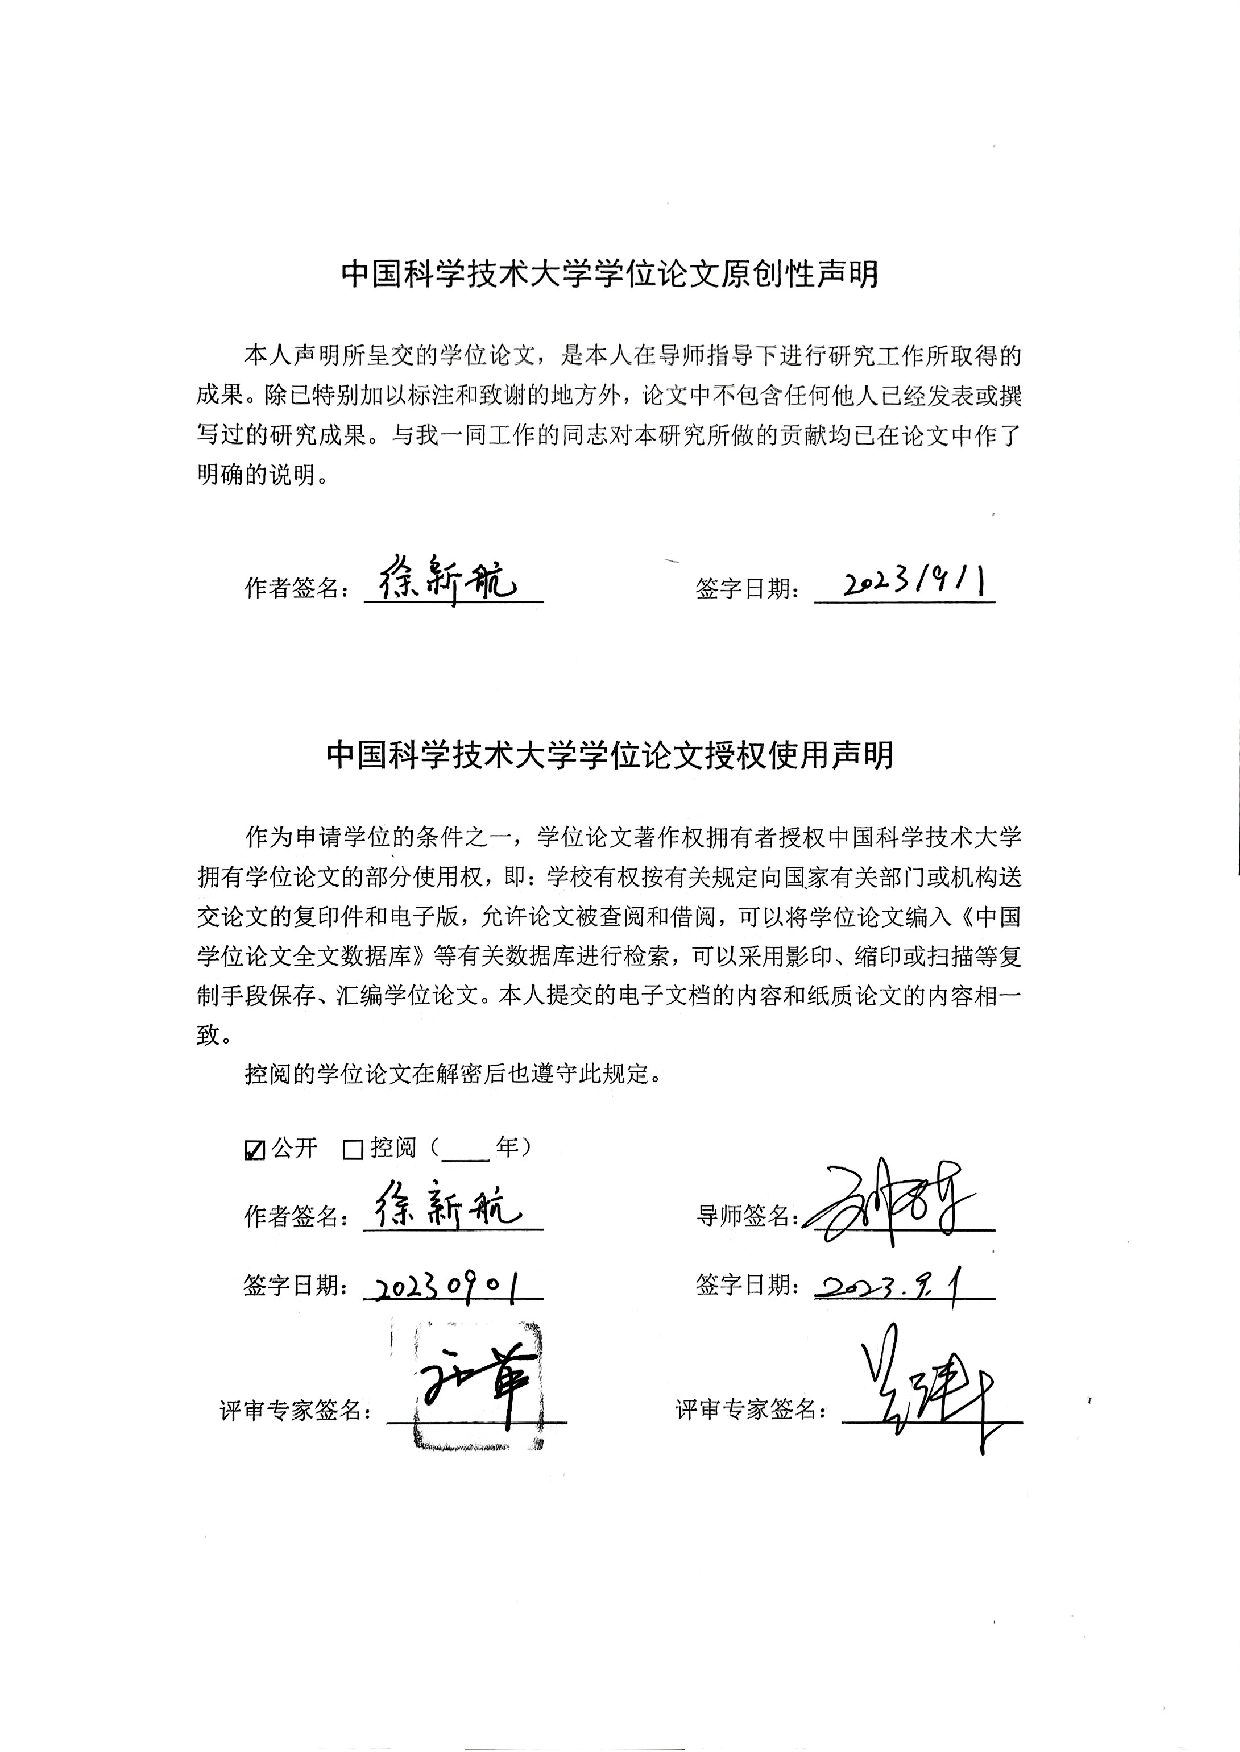
\includepdf[pages=1,fitpaper=true]{PDF_中国科学技术大学学位论文原创性声明.pdf}
\frontmatter
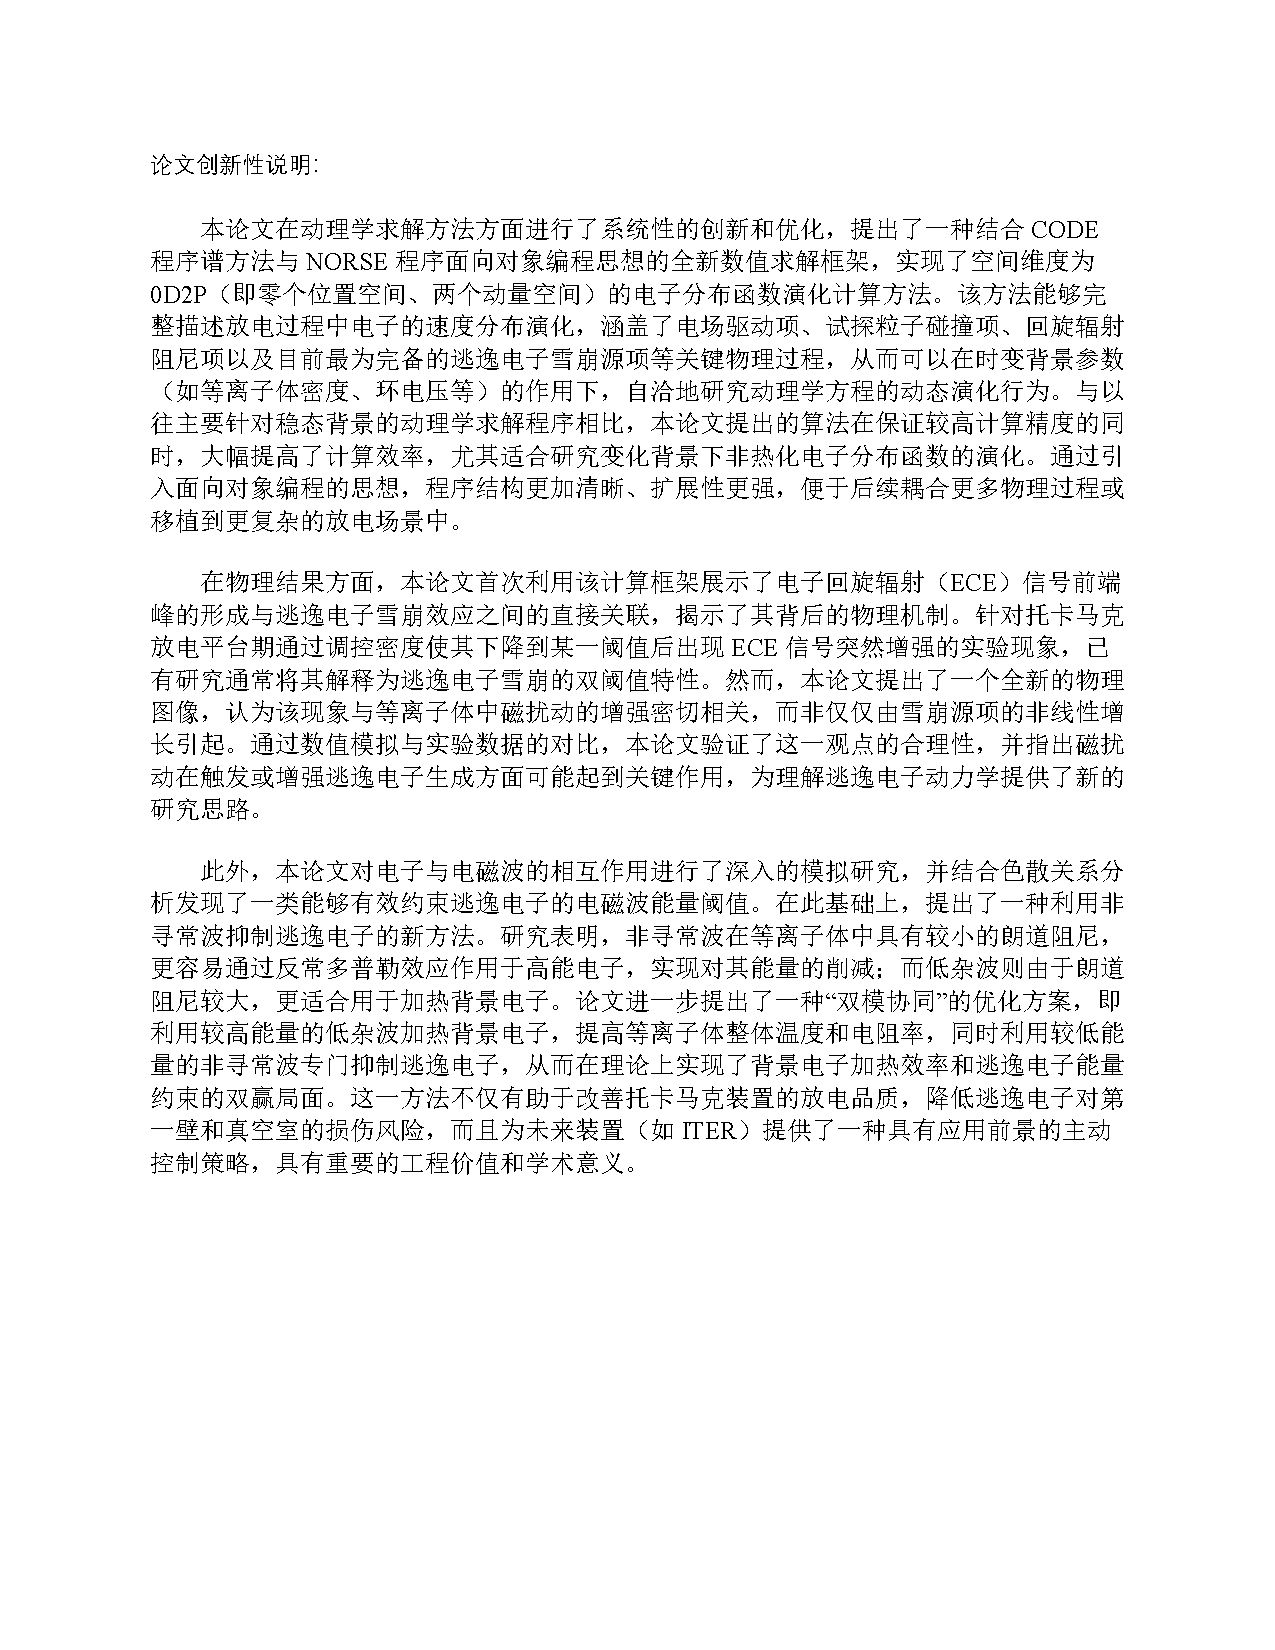
\includepdf[pages=1,fitpaper=true]{论文创新性说明.pdf}
%%

\frontmatter
% !TeX root = ../main.tex

\ustcsetup{
  keywords  = {电子回旋辐射;非热化电子;动理学;数值模拟;反常多普勒效应;逃逸电子},
  keywords* = {Electron Cycltron Emission,Non-thermal Electrons,Kinetic theory,Numerical simulation, Anomalous Doppler Effect,runaway electrons},
}

\begin{abstract}
 % 托卡马克放电过程中伴随大量的物理过程,这些过程互相耦合导致磁约束等离子体表现出繁杂丰富的实验现象。例如在EAST托卡马克电流爬升过程中,电子回旋辐射信号出现秒量级的前端峰结构并伴随着毫秒量级台阶结构,另一个现象是放电平台期密度下降到某个临界值时电子回旋辐射信号会突然开始暴增。除此之外,托卡马克在一定条件下会产生大量逃逸电子,高达MeV的高能逃逸电子不仅浪费欧姆储能,当其轰击在第一壁上还会对装置带来严重的破坏。随着放电参数的提高,逃逸电子问题对未来的聚变装置的影响也越发显著,但逃逸电子的动理学过程目前仍然有待进一步研究。逃逸电子的产生和电子回旋辐射的演化本质上都可以用分布函数来描述,而分布函数的演化又与动理学方程相关,为了理解反常电子回旋辐射现象的产生机制以及逃逸电子的动理学过程,本文通过对物理过程建模分析,利用数值驱动的方法根据诊断测量的背景参数驱动动理学模型运转,以此研究不同放电环境下电子回旋辐射的实验现象。\par
托卡马克中非热化电子直接与等离子体放电品质、装置安全运行等重要问题密切相关。研究非热电子的动理学机制及控制机理具有重要现实意义。非热电子在托卡马克放电过程中广泛存在,电子回旋辐射诊断对非热电子尤为敏感,在 EAST 托卡马克电流爬升过程中,非热化电子导致电子回旋辐射信号出现秒量级的前端峰结构和毫秒量级的台阶结构。在 EAST 托卡马克放电平台期,当密度下降到某个临界值时,电子回旋辐射信号也有时会突然暴增。本文基于实验测量的背景参数(如温度、密度、环电压等)通过动理学方程和电子回旋辐射数值诊断对以上实验现象展开了数值研究,以求探究电子回旋辐射实验数据背后更加深刻的物理过程。当托卡马克处于一定放电条件下时会产生大量逃逸电子,其中高达 MeV的高能逃逸电子不仅会消耗欧姆储能,还会对装置造成严重的破坏。随着放电参数的提高,逃逸电子问题对未来的聚变装置影响越来越大,亟需要有效可靠的手段抑制逃逸电子。因此本文对逃逸电子的控制问题展开了初步的探索。
\par
本文设计了从分布函数映射到回旋辐射强度的计算程序,为研究电子速度分布演化提供了可与实验参考的数值诊断平台。电子回旋辐射强度计算涉及了辐射率、吸收系数、辐射路径等问题,本文通过 B. Trubnikov 和 G. Bekefi 等科学家提出的理论完成了吸收系数和辐射率与分布函数关系的数值计算,结合辐射路径实现了电子回旋辐射强度和电子速度分布之间的定量计算。 为了计算电子速度分布的演化,本文考虑了均匀电场磁场(电场平行于磁场)背景条件下分布函数的动理学过程。动理学模型包含了电子碰撞项、辐射阻尼项、电子雪崩项、磁扰动扩散项等。最后通过标准模型和理论解对比,验证算法计算结果的准确性。 通过辐射输运计算程序和动理学程序,本文结合 EAST 实验中放电参数,对电子速度分布 演化和对应的回旋辐射进行求解,揭示了电子回旋辐射前端峰形成过程中逃逸电子雪崩机制参与的重要作用。针对放电平台期密度下降到某个临界值时,电子回旋辐射信号也有时会突然暴增的实验现象,本文确认了EAST托卡马克中密度降低时电子回旋辐射信号迅速上升的根本原因是磁扰动引起的非热电子损失项减少。通过数值模拟和实验数据进一步验证了这个结论。 最后本文研究反常多普勒效应的动力学过程,从单粒子运动出发,模拟了均匀背景下磁化电子和电磁波的相互作用过程。数值结果表明当电磁波电场强度超过背景静电场强度约 5倍,电子速度满足反常多普勒共振条件时,外界电磁波可将电子平行方向电场能量散射到垂直方向。同时电子还会激发出和背景电磁波相同性质的电磁波,电子平行方向速度此时不再被静电场加速。结合托卡马克装置中电磁波色散关系,对利用电磁波抑制逃逸电子方案的可行性进行了验证。该发现为磁约束装置运行中慢化逃逸电子提供了一种可能的方案。
\par
本文主要内容是独立开发完成了电子动理学数值计算程序及电子回旋辐射诊断数字仿真平台,并利用标准模型验证了程序的正确性。然后基于已开发的数值模拟程序,确认了EAST托卡马克中密度降低时电子回旋辐射信号迅速上升的根本原因是磁扰动引起的非热电子损失项减少;最后是基于保体积算法开发了单电子与外加电磁场相互作用的数值模拟程序。主要创新点是发现一定强度的电磁波可以通过反常多普勒共振效应抑制电子在平行磁场方向的加速,并提出了一种利用较低能量电磁波从托卡马克高场侧注入以控制托卡马克中逃逸电子能量的方法。

\end{abstract}

\begin{abstract*}
\par
Non-thermal electrons in tokamaks are directly associated with important issues such as plasma discharge quality and device safety. Investigating the kinetic mechanisms and control mechanisms of non-thermal electrons holds significant practical significance. Non-thermal electrons are widely present in tokamak discharge processes, and electron cyclotron emission diagnostics are particularly sensitive to non-thermal electrons. In the EAST tokamak, during the current ramp-up phase, the presence of non-thermalized electrons leads to the appearance of front-end peaks and millisecond-level step structures in the electron cyclotron emission signal. Additionally, during the discharge plateau phase in the EAST tokamak, there are instances where the electron cyclotron emission signal suddenly increases when the density drops to a critical value.
In this study, numerical investigations were conducted on the aforementioned experimental phenomena using background parameters measured during experiments, such as temperature, density, and loop voltage. By employing kinetic equations and numerical diagnostics of electron cyclotron emission, a deeper understanding of the underlying physical processes behind the experimental data was sought. When a tokamak operates under certain discharge conditions, a large number of runaway electrons are generated. Among them, high-energy runaway electrons reaching MeV levels not only consume Ohmic energy but also cause severe damage to the device. As discharge parameters increase, the impact of runaway electrons on future fusion devices becomes increasingly significant, necessitating effective and reliable means to suppress runaway electrons. Hence, this study conducted preliminary explorations on the control of runaway electrons.
\par
A calculation program was designed in this study to map the electron velocity distribution to the cyclotron radiation intensity, providing a numerical diagnostic platform that can be referenced against experiments to study the evolution of electron velocity distribution. The calculation of electron cyclotron radiation intensity involves issues such as radiation rate, absorption coefficient, and radiation path. In this study, numerical calculations of the absorption coefficient and radiation rate in relation to the distribution function were performed based on theories proposed by B. Trubnikov and G. Bekefi, among other scientists. By combining the radiation path, a quantitative calculation of the electron cyclotron radiation intensity and electron velocity distribution was achieved. To calculate the evolution of the electron velocity distribution, the study considered the kinetic processes of the distribution function under the background conditions of a uniform electric field and magnetic field (with the electric field parallel to the magnetic field). The kinetic model included electron collision terms, radiation damping terms, electron avalanche terms, and magnetic perturbation diffusion terms. The accuracy of the algorithm's calculation results was verified by comparing them with those of standard models and theoretical solutions. By utilizing radiation transport calculation programs and kinetic programs, this study combined discharge parameters from EAST experiments to solve the evolution of electron velocity distribution and its corresponding cyclotron radiation. The significant role played by the runaway electron avalanche mechanism in the formation of the front-end peak in electron cyclotron radiation was revealed. Regarding the experimental phenomenon where the electron cyclotron emission signal suddenly increases when the density drops to a critical value during the discharge plateau phase in the EAST tokamak, this study confirmed that the fundamental reason for the rapid rise in the electron cyclotron emission signal is the reduction of non-thermal electron loss caused by magnetic perturbations. This conclusion was further validated through numerical simulations and experimental data. Finally, this study investigated the dynamic process of anomalous Doppler effect and simulated the interaction between magnetized electrons and electromagnetic waves starting from the motion of individual particles under a uniform background. Numerical results indicate that when the electric field intensity of the electromagnetic wave exceeds approximately five times the intensity of the background electrostatic field and the electron velocity satisfies the condition for anomalous Doppler resonance, the external electromagnetic wave can scatter the energy of the electron's parallel electric field to the perpendicular direction. At the same time, electrons also excite electromagnetic waves with the same properties as the background electromagnetic waves, and the parallel velocity of the electrons is no longer accelerated by the electrostatic field. Combined with the dispersion relationship of electromagnetic waves in tokamak devices, the feasibility of using electromagnetic waves to suppress runaway electrons was verified. This discovery provides a potential approach for slowing down runaway electrons in magnetic confinement devices.
\par
The main content of this study involves the independent development of numerical calculation programs for electron kinetics and a digital simulation platform for electron cyclotron radiation diagnostics. The correctness of the programs was verified using standard models. Based on the developed numerical simulation program, the study confirmed that the fundamental reason for the rapid rise in the electron cyclotron emission signal when the density decreases in the EAST tokamak is the reduction of non-thermal electron loss caused by magnetic perturbations. Finally, a numerical simulation program was developed based on the conservation volume algorithm to simulate the interaction between individual electrons and external electromagnetic fields. The main innovation is the discovery that certain intensity of electromagnetic waves can suppress the acceleration of electrons in the direction of parallel magnetic field through the anomalous Doppler resonance effect. It also proposes a method to control the energy of runaway electrons in a tokamak by injecting lower energy electromagnetic waves from the high-field side.
\end{abstract*}















\tableofcontents
 \listoffigures
\listoftables
% !TeX root = ../main.tex

%\begin{notation}
%
%  \begin{notationlist}{2em}
%    \item[$\displaystyle a$] The number of angels per unit area
%    \item[$\displaystyle N$] The number of angels per needle point
%    \item[$\displaystyle A$] The area of the needle point
%    \item[$\displaystyle \sigma$] The total mass of angels per unit area
%    \item[$\displaystyle m$] The mass of one angel
%    \item[$\displaystyle \sum_{i=1}^n a_i$] The sum of $a_i$
%  \end{notationlist}
%
%\end{notation}

\begin{notation}

  \begin{notationlist}{2em}
    \item[$\displaystyle e$] 基本电荷
    \item[$\displaystyle m_e$] 电子质量
    \item[$\displaystyle m_p$] 质子质量
    \item[$\displaystyle m_i$] 离子质量
    \item[$\displaystyle \mu_0$] 真空磁导率
    \item[$\displaystyle \epsilon_0$] 真空介电常数
    \item[$\displaystyle c$] 真空光速
    \item[$\displaystyle n_e$] 电子数密度
    \item[$\displaystyle \vB$] 磁场
    \item[$\displaystyle \vE$] 电场
    \item[$\displaystyle \vJ$] 电流密度
    \item[$\displaystyle I_p$] 等离子电流
    \item[$\displaystyle IT$]   纵场电流

    \item[$\displaystyle T$] 温度  
    \item[$\displaystyle \omega_{c0}$] 静电子回旋频率    
    \item[$\displaystyle \omega_{ce}$] 动电子回旋频率
    \item[$\displaystyle \omega_{ci}$] 离子回旋频率
    \item[$\displaystyle \omega_{pe}$] (电子)等离子频率
    \item[$\displaystyle \omega_{pi}$] 离子等离子频率
    \item[$\displaystyle \omega_{LH}$] 下杂化频率
    \item[$\displaystyle \omega_{UH}$] 上杂化频率
    \item[$\displaystyle \omega_{R}$] 右旋截止频率
    \item[$\displaystyle \omega_L$] 左旋截止频率
    \item[$\displaystyle \tau_{cc}$] 相对论碰撞时间
    \item[$\displaystyle \tau_{ee}$] 热电子碰撞时间
    \item[$\displaystyle \Lambda$] 等离子体参数
    \item[$\displaystyle \ln\Lambda$] 库仑对数
  \end{notationlist}
\end{notation}


% 也可以使用 nomencl 宏包

% \printnomenclature

% \nomenclature{$\displaystyle a$}{The number of angels per unit are}
% \nomenclature{$\displaystyle N$}{The number of angels per needle point}
% \nomenclature{$\displaystyle A$}{The area of the needle point}
% \nomenclature{$\displaystyle \sigma$}{The total mass of angels per unit area}
% \nomenclature{$\displaystyle m$}{The mass of one angel}
% \nomenclature{$\displaystyle \sum_{i=1}^n a_i$}{The sum of $a_i$}


\mainmatter
% !TeX root = ../main.tex

\chapter{绪 论}

\section*{引言}
本文的研究主题是托卡马克(Tokamak)装置中非热化电子的演化过程及其对电子回旋辐射的影响。首先,介绍了可控核聚变的基本背景知识,为研究奠定物理基础;随后,详细讨论了托卡马克放电初期非热化电子的起源及其研究意义。接着,阐述了反常多普勒效应的物理机制\cite{RN1585}及其对电子速度分布的影响,并结合相关实验观测现象进行分析。通过上述内容,引出了本文的研究核心:非热化电子的动理学分析及其对电子回旋辐射特性的影响。
\section{可控核聚变}
传说在一万两千年前一个遥远的午后,有一只鸟,名叫毕方,飞到昆仑山上的一棵燧木上,当毕方啄木之时,燧木竟然生起火来,这一幕被山上燧人氏族人看到后深受震惊,后来燧人氏受毕方鸟的启发发明了钻木取火,开启了华夏璀璨文明。一万年后的今天,中国乃至世界依然在如何取火的问题上孜孜不倦地探索,只是现在是在原子核内部“钻木取火” ——可控核聚变。\par
核聚变是通过原子核聚合的方式释放热量。实现核聚变必须要达到一定的温度密度和约束时间,例如太阳主要通过p-p I 分支发生聚变反应,如\autoref{fig:ppI}所示,其反应方程如下:
\begin{equation*}
\begin{aligned}
&p+p\to{}_1^2\text{D}+e^{+}+\nu_e+1.442\MeV \\
&{}_1^2\text{D}+p\to {}_2^3\text{He}+\gamma+5.49\MeV \\
&{}_2^3\text{He}+{}_2^3\text{He}\to{}_2^4\text{He}+2p+12.859\MeV
\end{aligned}
\end{equation*}

\begin{figure}[ht]
\centering
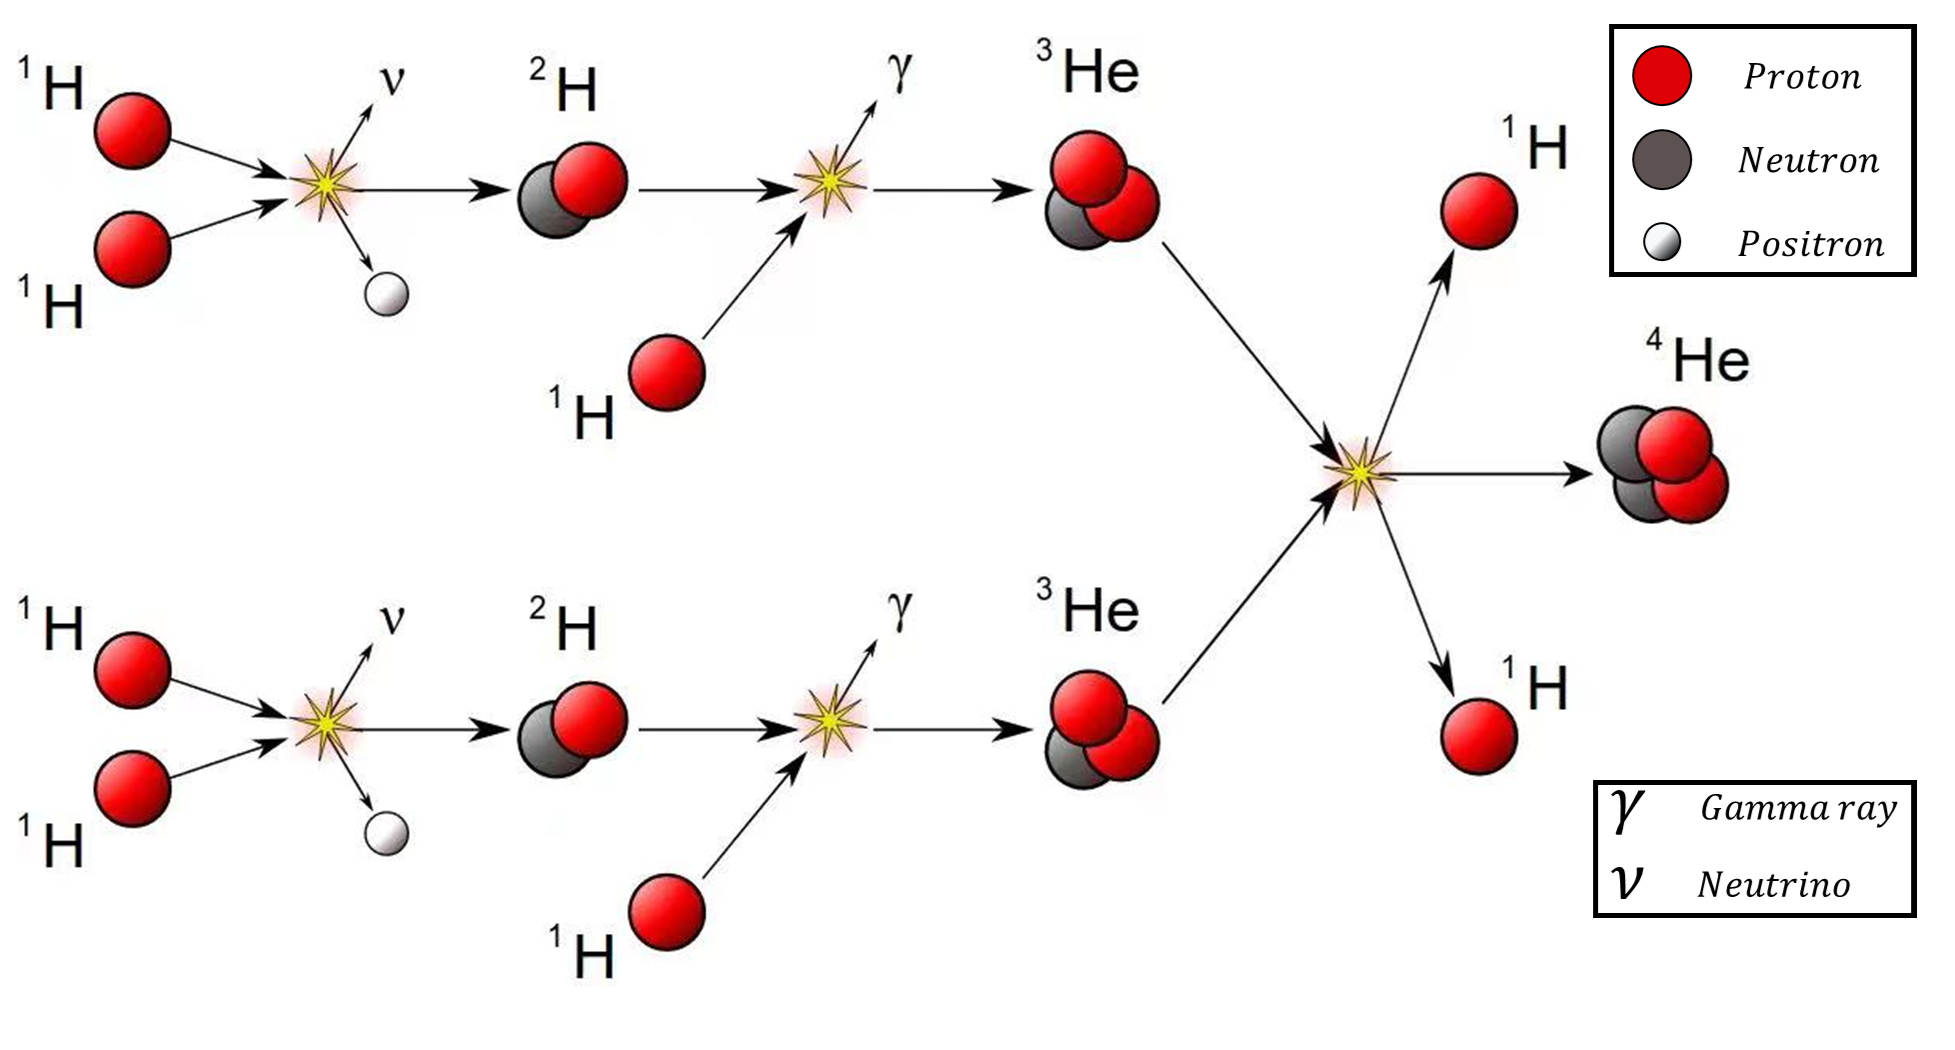
\includegraphics[width=14cm]{ppl_2.png}
\caption{\label{fig:ppI} p-p I 链式反应示意图,$^1H$代表质子,$^2H$代表氘核,$ν$代表电子中微子,
$^3He$代表氦-3 核,$^4He$代表氦-4 核,$γ$代表光子。反应朝箭头方向进行。\href{https://www.sun.org/encyclopedia/stars}{(https://www.sun.org/encyclopedia/stars)}
}
\end{figure}
\noindent     其中p代表质子,D代表氘核,e+代表正电子,$\nu_e$代表电子中微子,$^3He$代表氦-3核,$^4He$代表氦-4核,γ代表光子。反应按照箭头的方向进行。由于质子-质子衰变属于弱核力,反应效率很低,但是太阳的引力能长时间约束反应物,大量的反应物通过量子隧穿效应得以在太阳上能持续不断发生核聚变反应。然而地球上很难通过引力约束的方式产生受控核聚变,为了有效约束反应物,使之达到聚变反应条件,人们提出了惯性约束和磁约束等方式,其中磁约束中主流位型是托卡马克位型,如中国的EAST、美国的DIII-D以及未来的ITER。如\autoref{fig:tokamak}所示,托卡马克
\begin{figure}[ht]
\centering
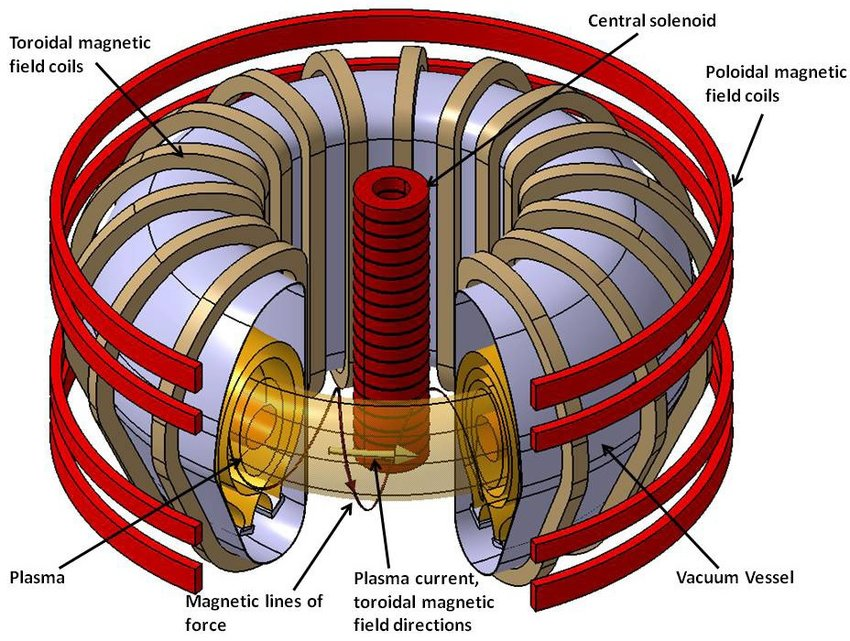
\includegraphics[width=12cm]{image2.jpeg}
\caption{\label{fig:tokamak} 托卡马克结构图\cite{RN950}}
\end{figure}
利用环向磁场和角向磁场将上亿度的等离子体约束在磁笼中,当密度、温度约束时间达到\href{https://www.energyencyclopedia.com/en/nuclear-fusion/thermonuclear-fusion/lawson-criterion}{劳森判据}时,即可实现自持的聚变燃烧。目前人们主要关注的聚变反应有$D-D$、$D-T$、$D-\text{He}^3$三种方式。\autoref{fig:D_D} 给出了它们的反应截面随温度的变化曲线,在温度较低时$D-T$反应相对于$D-D$和$D-\text{He}^3$具有更高的反应截面,高反应截面可以增加反应的概率和速率,从而提高反应效率,其相应的反应方程为:
\begin{equation*}
\begin{aligned}
&D+T\to\alpha(3.5\MeV)+n(14.1\MeV)\\
&D+D\to{}^3\text{He}(0.82\MeV)+n(2.45\MeV)\\
&D+{}^3\text{He}\to\alpha(3.6\MeV)+p^+(2.45\MeV)\\
\end{aligned}
\end{equation*}
海水中含有丰富的氘元素,根据氘氚反应方程可知3.8公升的海水可以产生相当于1135公升汽油的能量。面对未来的能源危机,受控核聚变为人类提供了一种绿色无限的能源。尽管有人称之为“永远的50年”,但能源的探索永不过时,因为我们的未来是星辰大海。
\begin{figure}[ht]
\centering
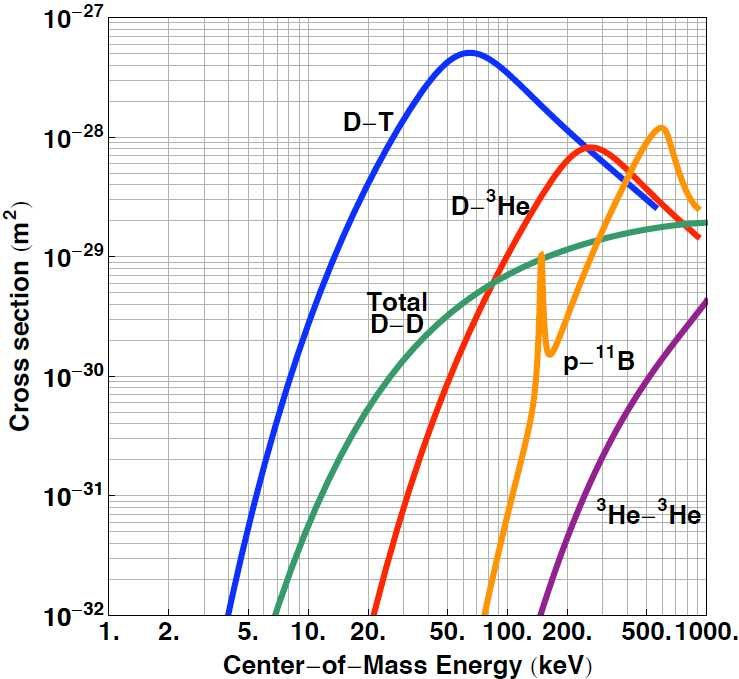
\includegraphics[width=12cm]{image3.jpeg}
\caption{\label{fig:D_D} $D-T$,$D-D$和$D-\text{He}^3$的反应截面,图片来自\cite{RN1698}}
\end{figure}
\clearpage
\section{托卡马克感应放电}
目前托卡马克放电主要通过中心螺线圈产生的感应电场实现对气体的电离并驱动带电粒子形成电流(如\autoref{fig:ohmdevice})。中心螺线圈感应放电一般分为三个阶段:电离或雪崩阶段、杂质烧蚀阶段和等离子体电流控制阶段\cite{RN2}。在托卡马克放电前中心螺线管预先储能,当放电指示下达时,中心螺线管通过电源和辅助电路的控制使电流开始下降,中心螺线管的磁通发生改变,在托卡马克环向会产生感应电场。关于该环电场强度的大小可以通过如下模型计算:中心螺线管外界电源电压为$V_{ps}$ ,外部电路的电阻为$R_{coil}$,电路电流为$I_{coil}$,根据电路基尔霍夫电压定律,中心螺线管的自感电压为$V_{coil}=V_{ps}-I_{coil}R_{coil}$,自感电压又可以表示为$V_{coil}=L_{coil}\frac{\dif I_{coil}}{\dif t}$,其中$L_{coil}$表示中心螺线管的自感系数,同时,考虑中心螺线管和等离子体之间的互感为M,绕大环方向一圈的环电压为$V_{loop}=M \frac{\dif I_{coil}}{\dif t}$,因此,$V_{loop}=MV_{coil}/L_{coil}$ ,在大半径为R处电场强度为$E=V_{loop}/2πR$。
\begin{figure}[ht]
\centering
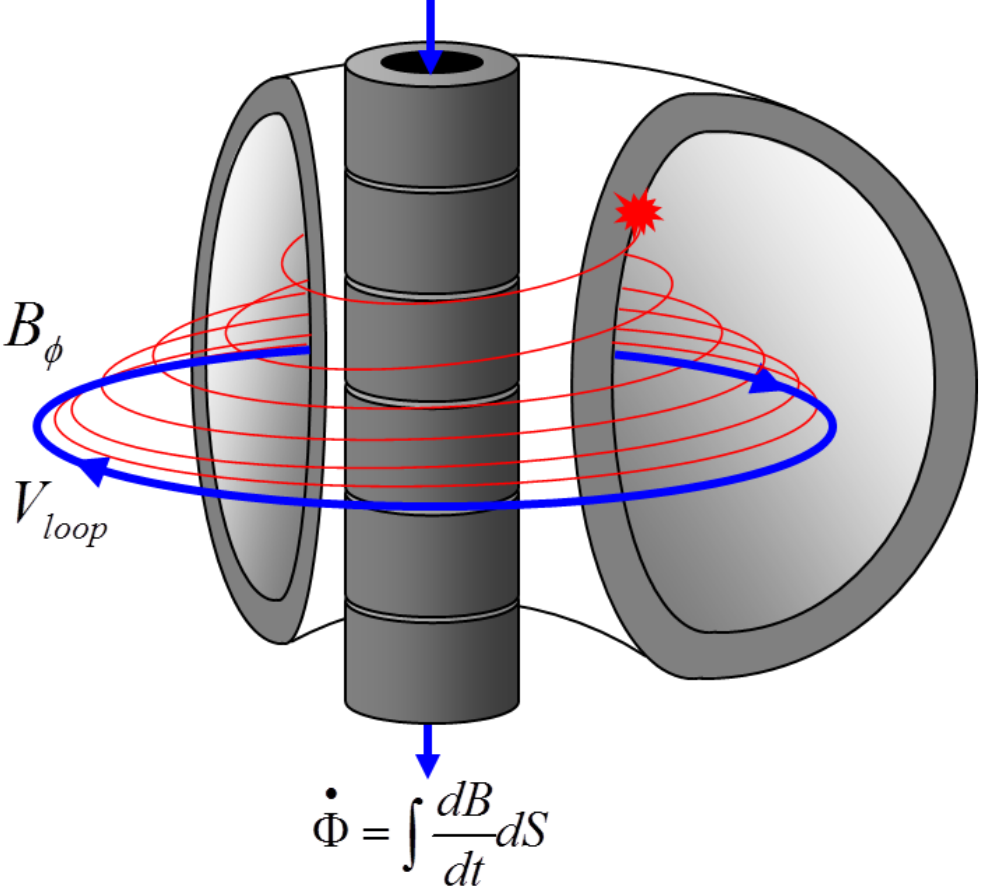
\includegraphics[width=12cm]{image4.png}
\caption{\label{fig:ohmdevice} 感应放电电子在环向磁场中的运动示意图\cite{RN951}}
\end{figure}
\par 托卡马克真空室中几乎一直存在自由电子,这些自由电子有可能来自于真空涨落,也有可能来自预电离的等离子体。放电启动时,这些自由电子在环电场作用下会被加速。当电子与下一个中性原子碰撞前动能超过$13.6\text{eV}$(氢原子的第一电离能,如果工作气体为氢气),电子就可能使中性原子电离并产生两个自由电子,新产生的电子会在环电场作用下继续加速,碰撞出更多的电子,这样的连锁反应过程称为汤森雪崩\cite{RN1234}。在雪崩过程中,单个电子单位路径产生α个自由电子,那么dx路径上就有d$n_e$=$αn_e $dx个电子产生,$n_e$表示电子密度,x表示沿电场方向的运动距离,积分得到具有指数增长的电子密度为$n_e=n_e (0) e^{αx}$,$α$表示第一汤森系数。击穿电离还涉及到击穿电场强度和预注入气体压强之间的关系,帕邢曲线描述了两板之间击穿电压和气压距离的关系,例如氦气的帕邢曲线如\autoref{fig:pxcurve}所示\cite{RN982},其中$V_b$表示电离击穿电压,d表示两板之间的距离,为了在最小的击穿电压下实现放电击穿必须对预填充气压做出合理的控制。托卡马克中电子绕中心
螺线管在大环方向上运动直到最后打在壁上所感受到的电压降V相当于帕邢曲线中的$V_b$,电子损失前运动的总路程称为连接长度L,类似于板间距d,如\autoref{fig:ohmdevice}红线所示。连接长度L与装置中的纵场$B_\phi$、杂
散场$B_s$ 以及小半径a有关,$L\sim a\cdot B_\phi/B_s $ ,例如在未来的ITER装置中,$B_\phi/B_s \sim10^{-3}$,$a=1-1.6m$,连接长度L约为1000m 。$\alpha/p$和$E/p$函数关系如\autoref{fig:pxcurve2} 所示\cite{RN1015}。 根据NSTX\cite{RN2}放电参数,$p\sim 5\times10^{-5}Torr$,$V_{loop}=2V/turn$,$α\sim10^{-2}/m$,电子在损失到真空壁前的约束路程必须要大于100m才能实现电子增益。托卡马克中电子在环向电场的驱动下主要沿环向磁场方向运动,但是由于磁力线弯曲、极向磁场、径向磁场梯度等因素,会使得电子在环向运动的同时还朝极向、径向运动,最终可能导致电子损失。为了在电子损失前有足够长的运动路程实现增益,在放电区域通常需要有零场区,这个位置只有环向磁场,极向磁场很小,电子在这个位置有足够长的连接长度,因此更容易电离击穿形成电流.
\begin{figure}[ht]
  \centering
  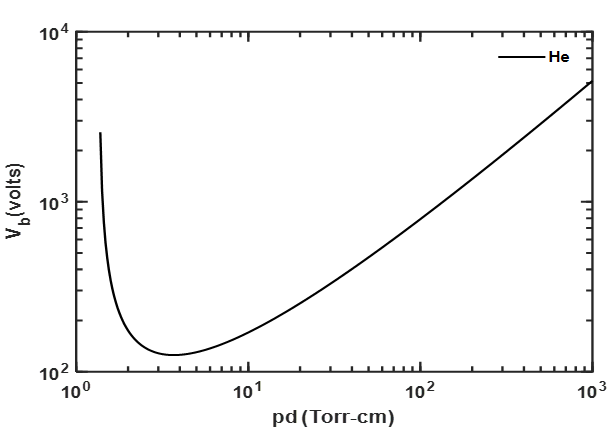
\includegraphics[width=12cm]{pxVb3.png}
  \caption{\label{fig:pxcurve} 氦气帕邢曲线图,pd表示气压×距离 }
\end{figure}


\begin{figure}[ht]
  \centering
  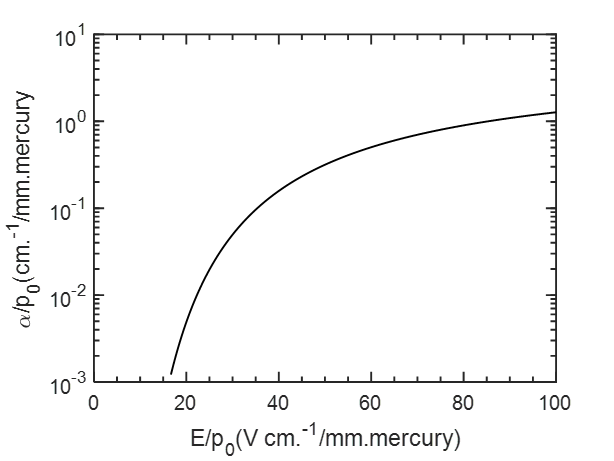
\includegraphics[width=12cm]{Ealpha2.png}
  \caption{\label{fig:pxcurve2} 电子在气体中单位路径产生的新电子数$\alpha$和电场E气压$p_0$的关系 }
\end{figure}

随着电离雪崩发生,中性气体的电离率越来越高,电子-电子的碰撞频率逐渐超过电子-中性气体的碰撞频率,当电离率超过$0.3\%$时,此时雪崩电离结束,进一步的电离过程是通过等离子体加热完成\cite{RN3}。在欧姆场加热等离子体过程中,除了电离消耗能量,杂质辐射会也会消耗能量,这些杂质主要来自壁材料如碳或铍氧,当杂质辐射能量和电离耗能超过欧姆注入的能量时,等离子体能量下降,电子重新和离子结合形成中性原子,最后导致放电失败。因此放电前通常会通过对内真空壁进行锂化处理、高温烘烤以及辉光放电清洗等手段降低壁中的碳氧等杂质,通过减少杂质或增加额外的注入功率,使放电继续维持下去。

杂质烧蚀过程中,等离子体电流也在爬升。当等离子体电流产生的极向磁场大于杂散场时,开放的磁力线将会闭合形成闭合磁面。电子绕螺旋闭合磁力线运动,其约束将会极大提升。当闭合磁面包含整个等离子体区域时电流产生的极向磁场将大于杂散场,即:
\begin{equation}
\frac{\mu_{o} I}{2 \pi a}>B_{s} \sim B_{\phi} \frac{a}{L} \rightarrow j=\frac{I}{\pi a^{2}}>B_{\phi} \frac{2}{\mu_{o} L}
\end{equation}
对于未来的ITER装置,杂散场$B_s=3mT$,连接长度L为1000m,纵场B为3T,小半径$a\sim1m$,等离子体电流$I$需要达到$15KA$才能形成放电区间完整的闭合磁面。\par
     磁面闭合后,在电流爬升中电子在环向场驱动过程下不断和周围的电子通过库伦散射交换能量,经过一定时间后大量电子开始呈现热分布的状态,此时等离子体具有了温度的概念。在纯欧姆放电条件下,等离子体通过欧姆加热机制提升温度。由于等离子体芯部约束高,一般情况下等离子体芯部温度上升更快,芯部电流也相对于更大。同向电流的pinch效应(洛伦兹力)使得等离子体有向内收缩的趋势,而压强梯度使得等离子体具有向外膨胀的趋势,二力平衡时等离子体达到稳定状态。还有一种情况也值得注意:由于欧姆加热效率与电阻率有关,温度越高电阻越低,随着等离子体芯部温度上升,芯部欧姆场加热效率也逐渐下降。携带电流的电子逐渐由热电子向非热化电子转移,而非热化电子主要为逃逸电子(关于逃逸电子在接下来的一小节会详细介绍)。由于逃逸电子碰撞阻尼小,该部分电子运动类似超导电子,类比伦敦第二方程可知逃逸电子会导致芯部感应电场下降,进而影响环向感应电场分布,改变环向电流分布。当满足一定条件时甚至会出现芯部电流低于边界电流的现象,也就是电流的趋肤效应。电流分布的空穴结构有可能导致撕裂模产生,破坏等离子体粒子约束\cite{duchs1972skin},也有可能会进一步提高等离子体的稳定性,促进聚变反应\cite{gourdain2009hollow}。因此放电初期对非热化电子的研究尤为重要。




%此时等离子体的平衡位型完全可由Grad-Shafranov方程描述,通过求解Grad-Shafranov方程获得的等离子体平衡位型为实验运行提供了重要参数。
    

\section{非热化电子产生机制}
	根据热力学定律,在没有外界影响下,一个热力学系统经过足够长时间后必然趋向于热分布,此时整个系统处于热平衡状态。对于托克马克中的电子,当电子速度分布通过碰撞散射达到热平衡分布时称为热电子,此时电子速度分布可以通过麦氏方程描述。但当电子速度分布偏离麦氏分布时称为非热化电子。导致电子速度偏离热分布的原因有很多,下面考虑欧姆场驱动下非热化电子的形成机制。\par
	通过试探粒子的方法可获得电子的等效阻尼力与电子动量的关系\cite{RN814,RN1817}(可参考附录\autoref{sec:A5})。如\autoref{fig:collisiondrag}中$F_c$所示,仅考虑库伦碰撞为电子加速过程中的等效阻力时,对于速度大于热速度的电子,库伦阻力与电子速度的平方成反比,当电子速度接近光速时受到的碰撞阻力达到最小值,如果电场力与这一最小碰撞阻力相当,则称该电场为Connor电场\cite{RN1875},凡是小于Connor电场的情况下均不可能存在逃逸电子,因此Connor电场也成为逃逸电子最小临界电场。当电场大于Conner电场时,碰撞阻尼小于电场力的电子将会受到加速,在加速过程中碰撞阻尼继续减小,最终电子将不断加速获得极高的能量, 因此该部分非热化电子称为逃逸电子。 然而实际情况下逃逸电场临界值通常大于Conner电场,这是因为存在磁场时,电子回旋辐射阻力会阻碍电子逃逸。如\autoref{fig:collisiondrag}中$F_{rad}$所示,电子回旋辐射阻尼$F_{rad}$随着电子速度增加而迅速上升,单电子其受到的总阻力为$F=F_{rad}+F_c$,这时电子的最小临界电场为$E_c^*$显然要高于$E_c$。当电场强度$E>E_c^*$时,处于动量区间$[p_1,p_2]$将发生逃逸,最终聚集在$p_2$点。在等离子体温度为$T_e$中电子的最大碰撞阻尼为热速度$v\approx v_{th}$所对应的平衡电场$E_s$,而与$E_s$同出一源的就是Dreicer电场
	\begin{equation}\label{eq:Dreicer_Field}
E_D=\frac{n_ee^3ln\Lambda}{4\pi \epsilon_0^2T_e}
\end{equation}
	Dreicer电场命名是为了纪念第一位研究等离子体中逃逸现象的科学家H.Dreicer\cite{RN954}。当电场强度达到$E_s\approx0.2E_D$时,整个等离子体中的电子都将发生逃逸,电子速度分布快速偏离麦氏分布,因此该电场称为side-away电场阈值。当电场只有百分之几的$E_D$,只有少量电子发生逃逸,刚刚逃逸出去的电子又会由于主体电子的扩散而得到补充,而主体电子的热分布特征并不会由于少量扩散而被改变,因此这部分少量的逃逸电子将会获得稳定的增长,这种逃逸电子的产生机制称为初级逃逸电子或Dreicer逃逸。
\begin{figure}[ht]
  \centering
  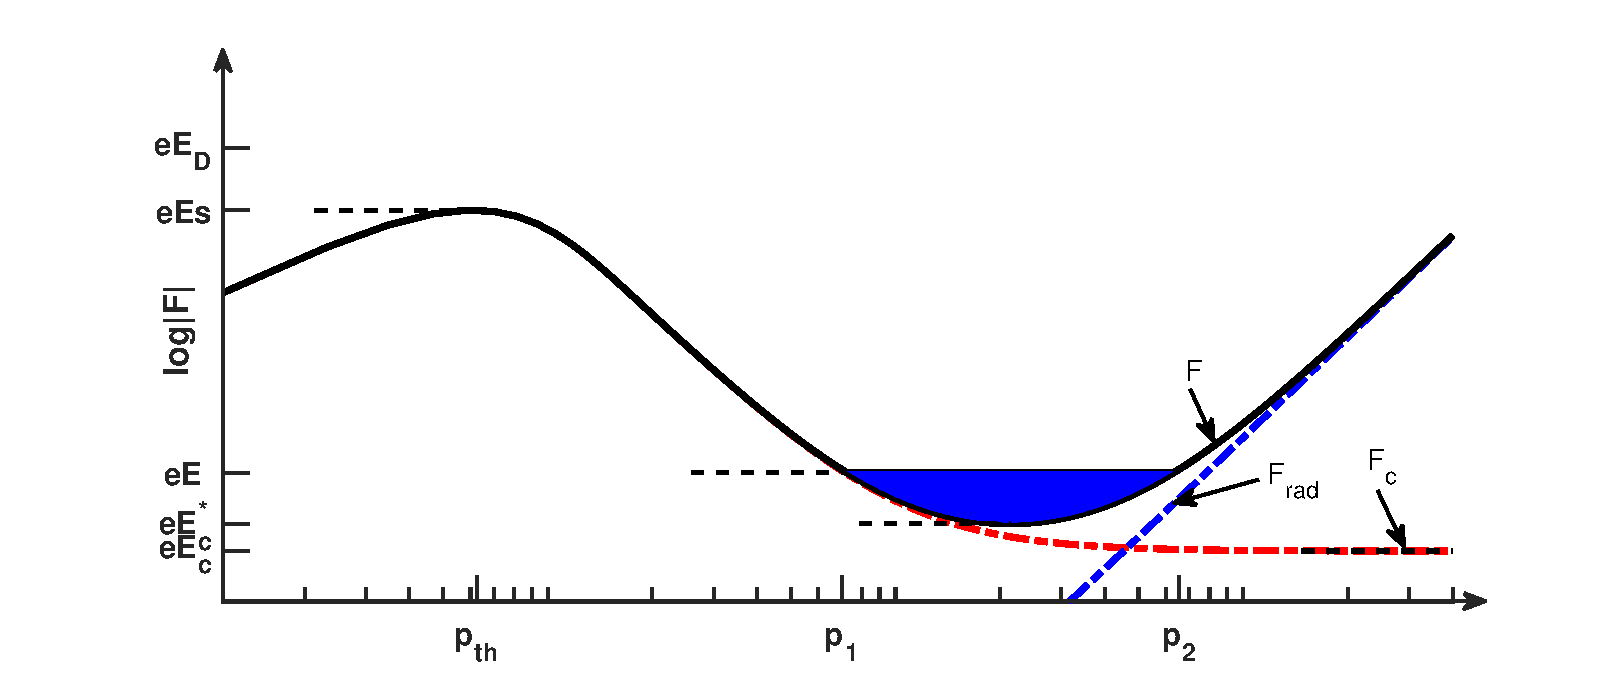
\includegraphics[width=16cm]{image7.eps}
  \caption{\label{fig:collisiondrag} 库伦碰撞阻力$F_c$、辐射阻力$F_{rad}$以及合力$F$随动量分布 }
\end{figure} 
\par
除了以上讨论的电场驱动电子逃逸过程,逃逸电子的另一种产生机制是通过大角度碰撞,也称为雪崩机制\cite{RN1793}。这种机制可以简单如下描述:一个具有高能量的逃逸电子和热电子发生大角度碰撞,碰撞后的两个电子速度均超过了临界速度然后形成两个逃逸电子,然后一生二,二生四,逃逸电子的数量就以雪崩指数增长。当然不是所有逃逸电子都能发生雪崩机制,在等离子体中由于辐射效应以及各种不稳定性限制导致逃逸电子存在能量上限\cite{RN874}。当系统中具有最大能量的电子和热电子碰撞后仍然不足以使碰撞后的两个电子都大于逃逸的速度,雪崩效应就不会发生。只有当电场大于一定值,逃逸电子能量足以产生逃逸电子对,雪崩效应才会产生。Aleynikov通过近似理论计算了有效电荷数Z为5,密度为$10^{20}~m^{-3}$,温度为$1~KeV$,磁场为$1.81~T$雪崩电场阈值$E_a$约为$1.8E_c$。然而后来基于玻尔兹曼碰撞算符数值模拟到的结果却表明不存在雪崩电场阈值\cite{RN1811},该部分内容会在\autoref{sec:no_growth}讨论密度下降过程回旋辐射问题时有详细讨论。

综上所述逃逸电子的产生存在两个临界电场:$E_c^*$表示产生逃逸电子所需最低电场;$E_s$表示所有电子均发生逃逸的临界电场,此时放电称为side-away放电。由于逃逸电子的能量上可达几十MeV,当其轰击到装置内壁时会对装置造成严重破坏,因此在放电过程中对逃逸电子的控制格外重要。如果能通过某种机制把平行磁场方向的电子动能转换到垂直方向,增大辐射阻尼的同时也增大了电子运动轨道长度,进而抑制逃逸电子的产生,对保护装置\cite{RN1866}和实现聚变均有所裨益。我们将在论文的\autoref{sec:simulationVPA}对这一机制进行详细讨论。

辅助加热也是非热化电子产生的重要途径。如低杂波加热过程中,电子速度和低杂波相速度满足共振条件时电子就会通过朗道阻尼获得能量成为非热化电子。 如\autoref{fig:nonths}所示,非热化电子会对电流分布产生影响,驱动MHD不稳定性,MHD不稳定性产生的磁扰动又会感应新的电场进一步影响非热化电子的产生。这种种关系或正反馈或负反馈构成了复杂多变的等离子体环境。托卡马克许多物理过程中都与非热化电子密切相关,如ELM\cite{RN1868}、Sawtooth\cite{RN1917}、Disruption\cite{RN985}等过程中都会产生非热化电子,而非热化电子对等离子体反常输运\cite{RN986}、误差场的穿透不稳定性\cite{RN987}、等离子体的加热过程\cite{RN1697}也有重要影响。

在纯感应放电过程中,逃逸电子的形成过程可以解释电子为什么会在平行磁场方向上产生MeV的动能,但无法解释实验中非热化电子垂直方向能量为什么可以达到百keV\cite{RN726}。首先可以排除是欧姆加热机制,因为热电子的温度通常只有keV,温度越高电子库伦碰撞频率越低,无法通过库伦碰撞产生百keV的能量。在垂直磁场方向具有百keV能量的非热化电子是如何产生的?关于这个问题目前有以下解释:
\begin{itemize}
\item 无碰撞散射过程\cite{RN1794} \par
由于托卡马克中磁场具有螺旋结构,电子在运动过程中感受到的磁场环境是不断变化的,导致电子的磁矩不再守恒,平行磁场方向加速的电子被背景磁场散射导致垂直磁场方向动能增大。
\item 电子雪崩过程\cite{RN1793} \par
背景电子被逃逸电子碰撞产生的大角度散射也是导致电子垂直方向能量升高的原因。
\item 反常多普勒效应(ADE,Anomalous Doppler Effect)\par
反常多普勒效应是电子和波相互作用产生的一种不稳定性。笼统地解释是在电场的驱动下,逃逸电子的能量逐渐增大,当能量达到一定阈值时,满足$ω-\vk\cdot \vv+nω_{ce}=0$\cite{RN1757}共振条件的波就会被激发出来。当n>0时对应反常多普勒共振,被激发出的波又会反过来作用于逃逸电子导致电子平行磁场方向的能量迅速转移到垂直磁场方向上,这样逃逸电子在垂直磁场方向的能量就会快速增加,这里ω表示激发出的波,$k_z$表示沿磁场方向的波矢,$v_z$表示电子平行磁场方向的速度,$ω_{ce}$表示电子回旋频率,n表示共振阶数。
\end{itemize}

\begin{figure}[ht]
  \centering
  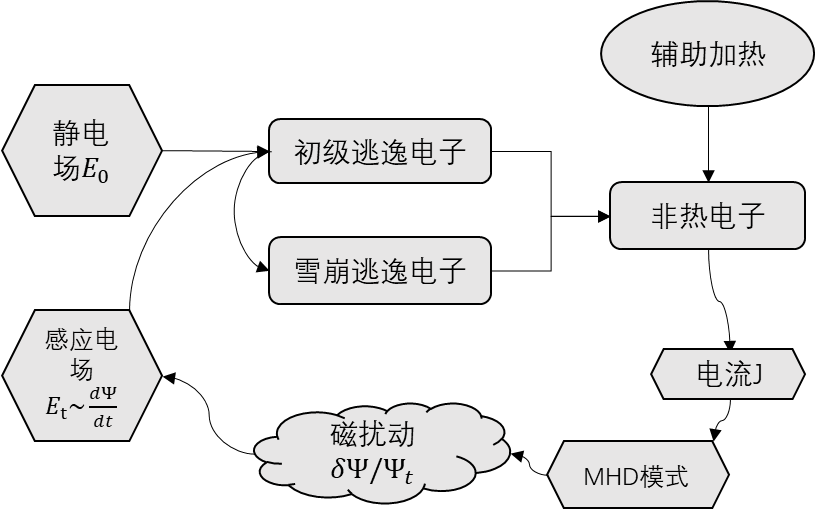
\includegraphics[width=12cm]{image8.png}
  \caption{\label{fig:nonths} 非热电子产生途径示意图 }
\end{figure}
那么ADE为什么会导致电子动量的快速散射?其物理机制是什么?关于这些问题目前的分析大都是建立在准线性理论分析上\cite{RN1801},从速度分布函数的演化角度解释散射,但ADE的物理本质并没有得到很好的理解,本文将在\autoref{sec:ewmele}对ADE效应的物理本质展开研究。
\par ADE机制与其它两种机制的最大区别就是存在一个由非热电子本身驱动的波。在托卡马克实验中已经有很多与ADE机制相吻合的实验观测\cite{RN975,RN798,RN786,RN1868},其中最明显莫过于放电初期的电子回旋辐射,我们将在第二章具体展开讨论。

\section{反常多普勒效应}\label{sec:quantum}
ADE是电子和波相互作用产生的一种不稳定性\cite{RN782},当电子在磁场中运动时,这种不稳定性会导致电子平行磁场方向的能量迅速散射到垂直磁场方向上。ADE效应最早是Ginzburg\cite{RN1352}, Tamm\cite{RN2008}以及I.M.Frank\cite{RN2009}提出的理论猜想,并且Tamm和I.M.Frank在1958年诺贝尔获奖报告上详细介绍了ADE理论。现在简单介绍这一不同寻常的现象:\par
如\autoref{fig:cherenkov}所示,当带电粒子以超过介质中光速的速度穿过介质时,将在介质内产生诱导电流。这些诱导电流会激发次波,并与运动粒子的电磁场相互干涉,从而产生切伦科夫辐射(Cerenkov Radiation\cite{RN1861})。此时辐射波矢k的传播方向只能沿着切伦科夫辐射角$cos(θ_0)=c/(vn(\omega))=\frac{c'}{v}=\frac{\omega}{kv}$。现在我们考虑把自由带电粒子替换成具有内能和动能的系统(如一个运动的振子或一个沿磁力线运动的回旋电子等)。如\autoref{fig:radreg}所示,该系统在折射率为$n(\omega)$的空间中超光速运动($v>c/n(ω) $)并辐射出具有角频率为$ω$的光子(图中$θ$表示光子辐射方向$\vk$和运动方向$\vv$的夹角),此时光子的方向可以沿任意方向,不依赖于次波叠加干涉。根据能量守恒和动量守恒关系,我们有
\begin{figure}[ht]
\centering
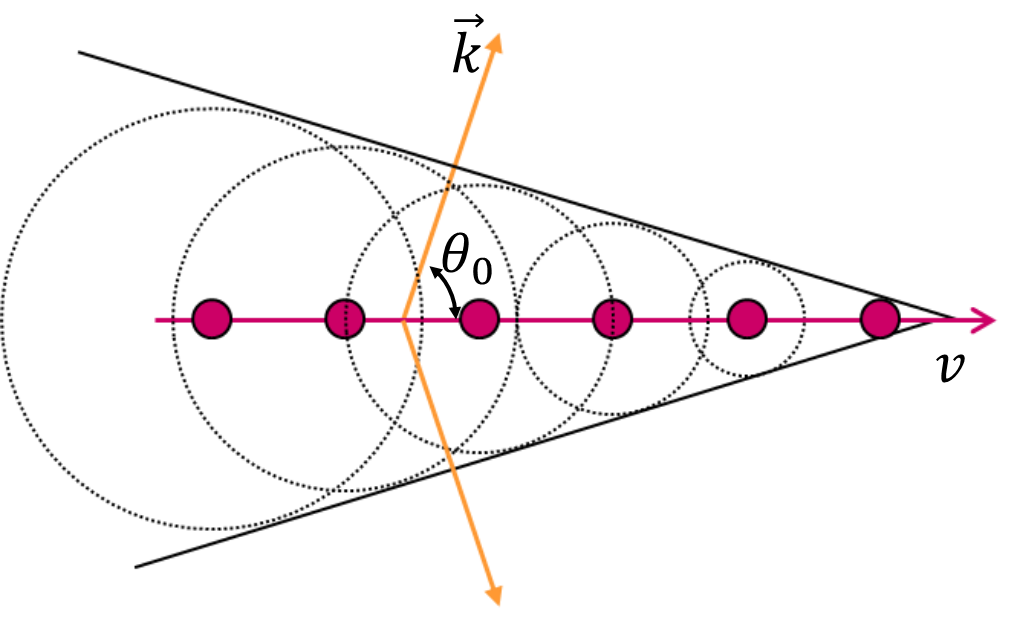
\includegraphics[width=12cm]{cherenkov.png}
\caption{\label{fig:cherenkov}实验室坐标系下粒子速度为$v$时切伦科夫辐射图\href{http://large.stanford.edu/courses/2014/ph241/alaeian2/}{(http://large.stanford.edu/courses/2014/ph241/alaeian2/)}		}
\end{figure}
\begin{figure}
\centering
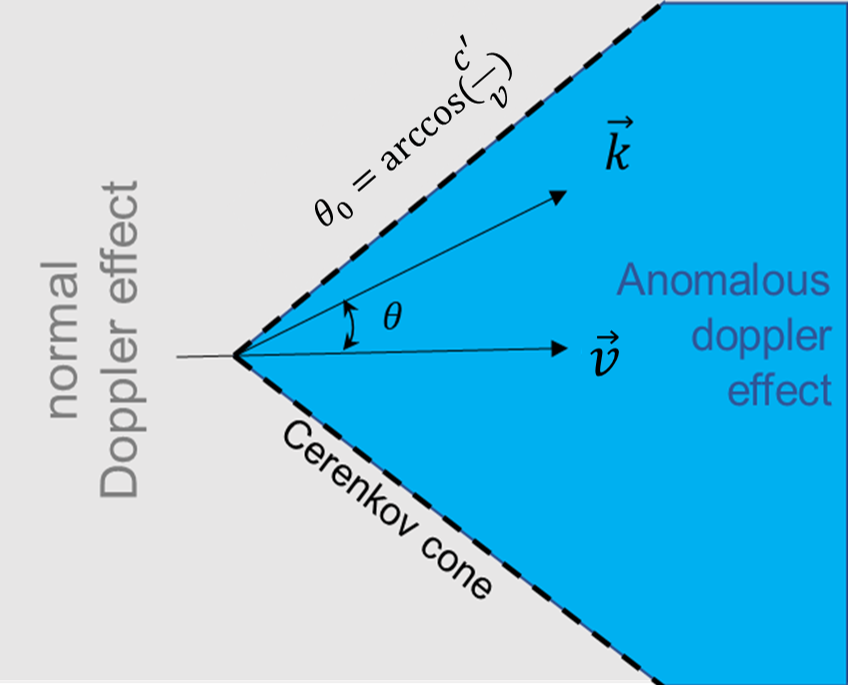
\includegraphics[width=12cm]{image21.png}
\caption{\label{fig:radreg}实验室坐标系下不同类型辐射区间分布,图片改自(X.H.Shi\&X.Lin)\cite{shi2018superlight}}
\end{figure}
\begin{equation}\label{eq:UT}
\begin{aligned}
T_1+U_1&=\hbar \omega+T_2+U_2 \\
\vp_1&=\vp_2+\hbar \vk 
\end{aligned}
\end{equation}

其中$T_1$和$U_1$表示系统初始具有的动能和内能,$T_2$和$U_2$表示辐射出光子后系统具有的动能和内能。考虑到光子能量远远小于系统具有的动能,$ℏω\ll T_1$,系统损失的动能可表示为$ΔT_{12}=T_1-T_2=Δ\vp\cdot\vv$,其中$\vv$表示辐射光子前系统的运动速度,$Δ\vp=\vp_1-\vp_2=\hbar\vk$。根据\autoref{eq:UT},我们有
\begin{equation}
\begin{aligned}
\Delta U_{21}=&ΔT_{12}-\hbar\omega\\
=&\hbar \vk \cdot \vv-\hbar \omega \\ 
=&\hbar \omega\left(\frac{k v \cos \theta}{\omega}-1\right)
\end{aligned}
\end{equation}
这里$ω/k=c/n(ω)=c'$ ,$\Delta U_{21}=U_2-U_1$。从方程中我们可以得到三点重要信息:\\
1.当$θ<θ_0 ,ΔU_{21}>0$,系统损失的动能转化为光子能量和系统的内能;\\
2.当$θ=θ_0,ΔU_{21}=0$,系统损失的动能完全转化为光子能量;\\
3.当$θ>θ_0,ΔU_{21}<0$, 系统通过消耗自身的内能和动能产生光子。\\

根据$ΔU_{21}$的正负,我们把辐射分为三种效应,其中$ΔU_{21}<0$称之为多普勒效应(NDE,Normal Doppler Effect),多普勒效应会消耗自身的内能和动能;$ΔU_{21}>0$为反常多普勒效应;$ΔU_{21}=0$称之为切伦科夫效应。当系统速度超光速$(v>c/n)$时,这三种效应均有可能产生,而当系统速度小于光速时$(v<c/n)$,只存在多普勒效应。
   \par 现在我们考虑这样一个特殊的系统:均匀磁场背景下平行于磁场方向运动的回旋电子。在该系统中,沿磁场方向电子以速度$v$自由运动,电子在垂直磁场方向上具有微小的速度$v_⊥$,假设在背景磁场强度为$B$的电子回旋能量(相当于内能)改变量满足量子化 \cite{RN1969}
\begin{equation}
\Delta U_{21} = n \hbar \omega_{ce},\omega_{ce}= \frac{eB}{m_e}
\end{equation}
这里$m_e$表示电子质量,$n=0,±1,±2,……$根据能量守恒定律,我们有:
\begin{equation}\label{eq:quantum energy}
ℏ\vk \cdot \vv=ℏω+nℏω_{ce}
\end{equation}
或
\begin{equation}
ω-\vk\cdot\vv=-nω_{ce}
\end{equation}
其中$ℏ\vk \cdot \vv$表示损失的动能,$ℏω$表示产生光子的能量,$nℏω_{ce}$表示电子回旋内能增加量($\Delta U_{21}$),$n$为整数。\autoref{eq:quantum energy}所包含的物理是:损失的动能$ℏ\vk \cdot \vv$转化为系统的内能$nℏω_{ce}$和光子能量$ℏω$。当$n<0$时对应多普勒效应,电子辐射光子后动能和回旋内能均降低;当$n=0$时对应切伦科夫效应,辐射的光子不会导致电子回旋内能任何改变;当$n>0$时对应ADE,根据能量方程$ℏ\vk\cdot\vv=ℏω+nℏω_{ce}$,电子平行方向动能的变化量转化为光子能量和增加的回旋内能。以上通过量子效应解释了ADE效应的能量转移特征,也可以从经典力学角度来考虑ADE的物理过程,我们将在论文\autoref{sec:ewmele}介绍磁化电子和电磁波相互作用时对ADE效应的力学机制进一步探究。根据ADE效应,如果在辐射光子前电子没有回旋内能只有平行方向的动能,那么在辐射光子后电子平行磁场方向动能将会向垂直方向转移。例如在电子束流实验中,ADE会使电子束流单一的速度方向发生弥散,这些现象已经被实验验证\cite{RN798,RN1862}。
\begin{figure}[ht]
\centering
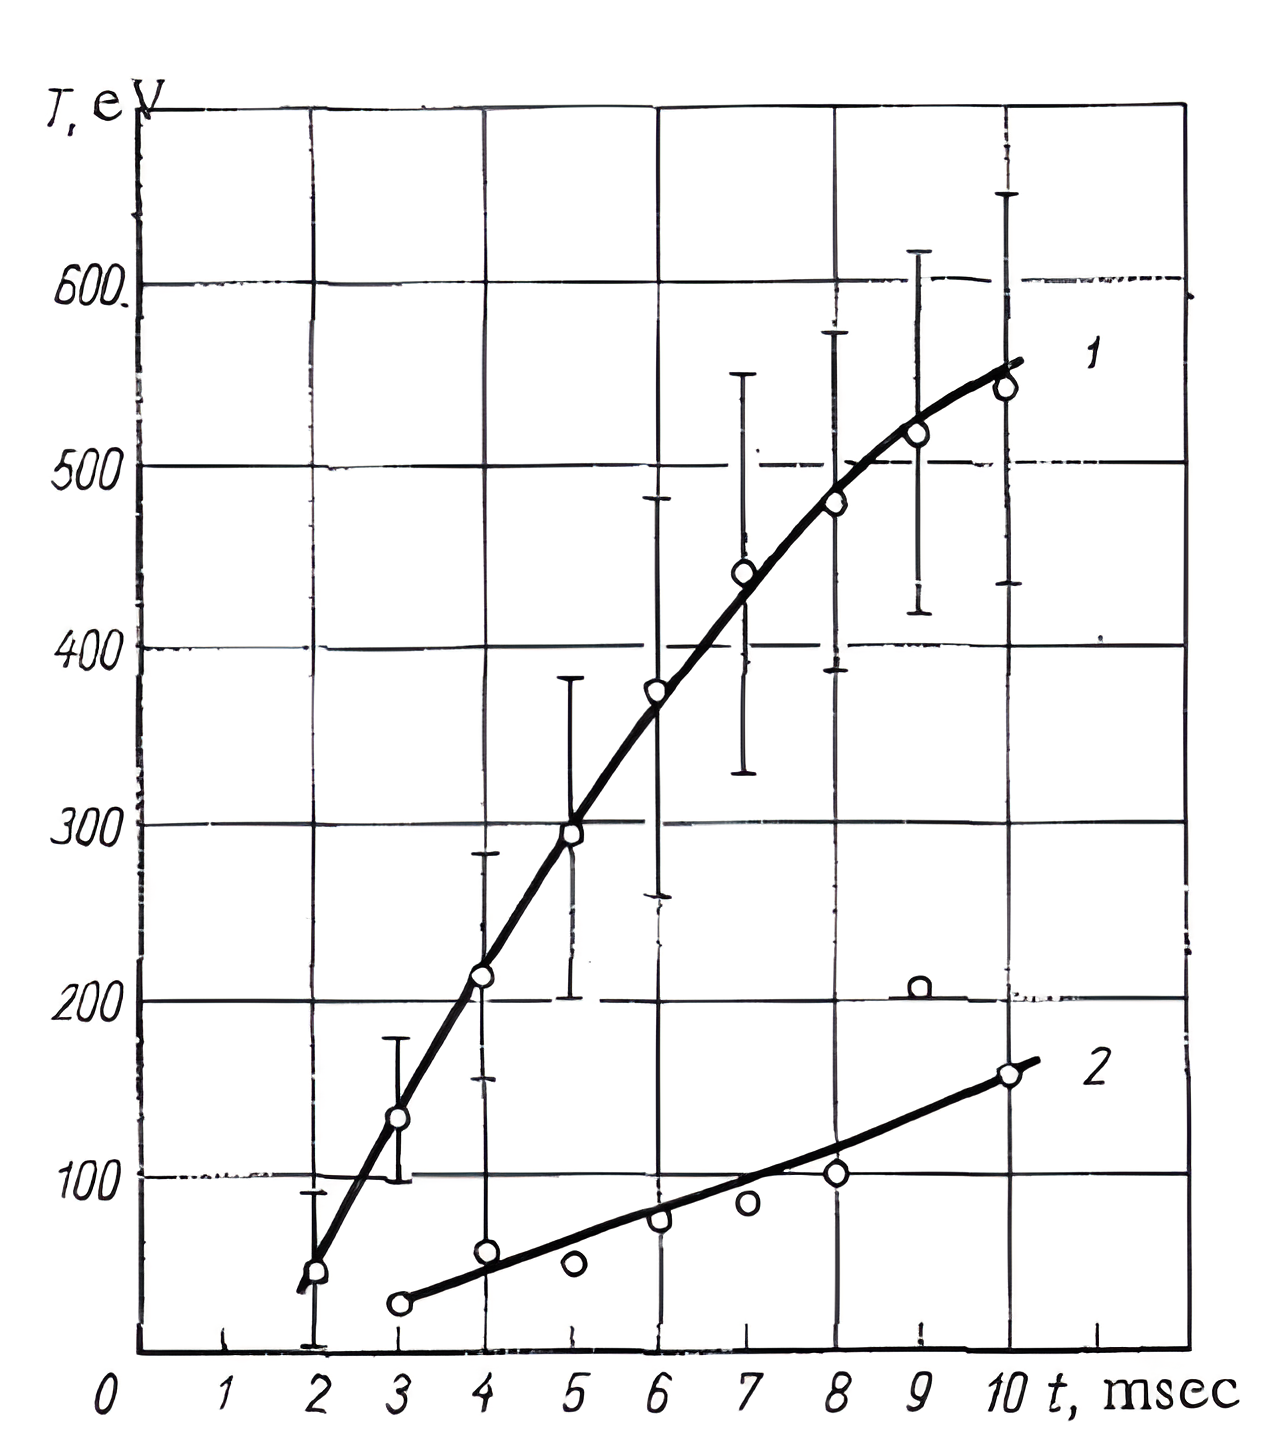
\includegraphics[width=10cm]{image22_1.png}
\caption{\label{fig:LAA}曲线1:抗磁性效应测量的$T_e + T_i$;曲线2:通过电导率测量的电子温度$T_{eσ}$}
\end{figure}
\par
1967年,前苏联L. A. Artimovich在 T-3托卡马克装置和TM-3托卡马克装置中分别用逆磁效应和经典等离子体电导率测量等离子体温度\cite{RN1863}。逆磁效应是磁化等离子体中常见的现象,其原因是因为电子和离子自旋产生的磁场方向和背景磁场相反,当电子或离子温度越高,逆磁效应越加显著,因此
可以通过测量托卡马克环向磁通的变化量反推出等离子体温度,同时通过测量环电压和等离子体电流可算出等离子体平均电导率,根据经典电导率和温度之间的关系同样可以推导出等离子体温度。如\autoref{fig:LAA}实验发现,通过逆磁效应测出的温度远大于等离子体电导率测出的温度 ,反过来说通过逆磁温度推导出来的电导率远大于实验测得的电导率,由于缺少合理的物理解释,对这种低于经典电导率的实验现象当时称为反常电导率。

\par 1968, B. B. KADOMTSEV指出L. A. Artimovich测到的反常电导率是由于ADE造成\cite{RN964},由于沿平行磁场方向运动的电子在ADE作用下电子向垂直磁场方向散射,导致逆磁效应增加,使得根据逆磁效应得到的电导率高于真实电导率。同年V. D. SHAPIRO\cite{RN1425}提出了等离子体中反常多普勒过程的准线性理论,等离子体中ADE开始逐渐引起人们重视。
\par 1971年E. G. SHUSTIN利用微波天线和静电场能量分析器研究磁场背景下真空放电管等离子体束不稳定性\cite{RN786},如\autoref{fig:EGS1}所示,\autoref{fig:EGS1}上图是整个系统框架,包括真空放电管,可移动微波探
\begin{figure}[ht]
\centering
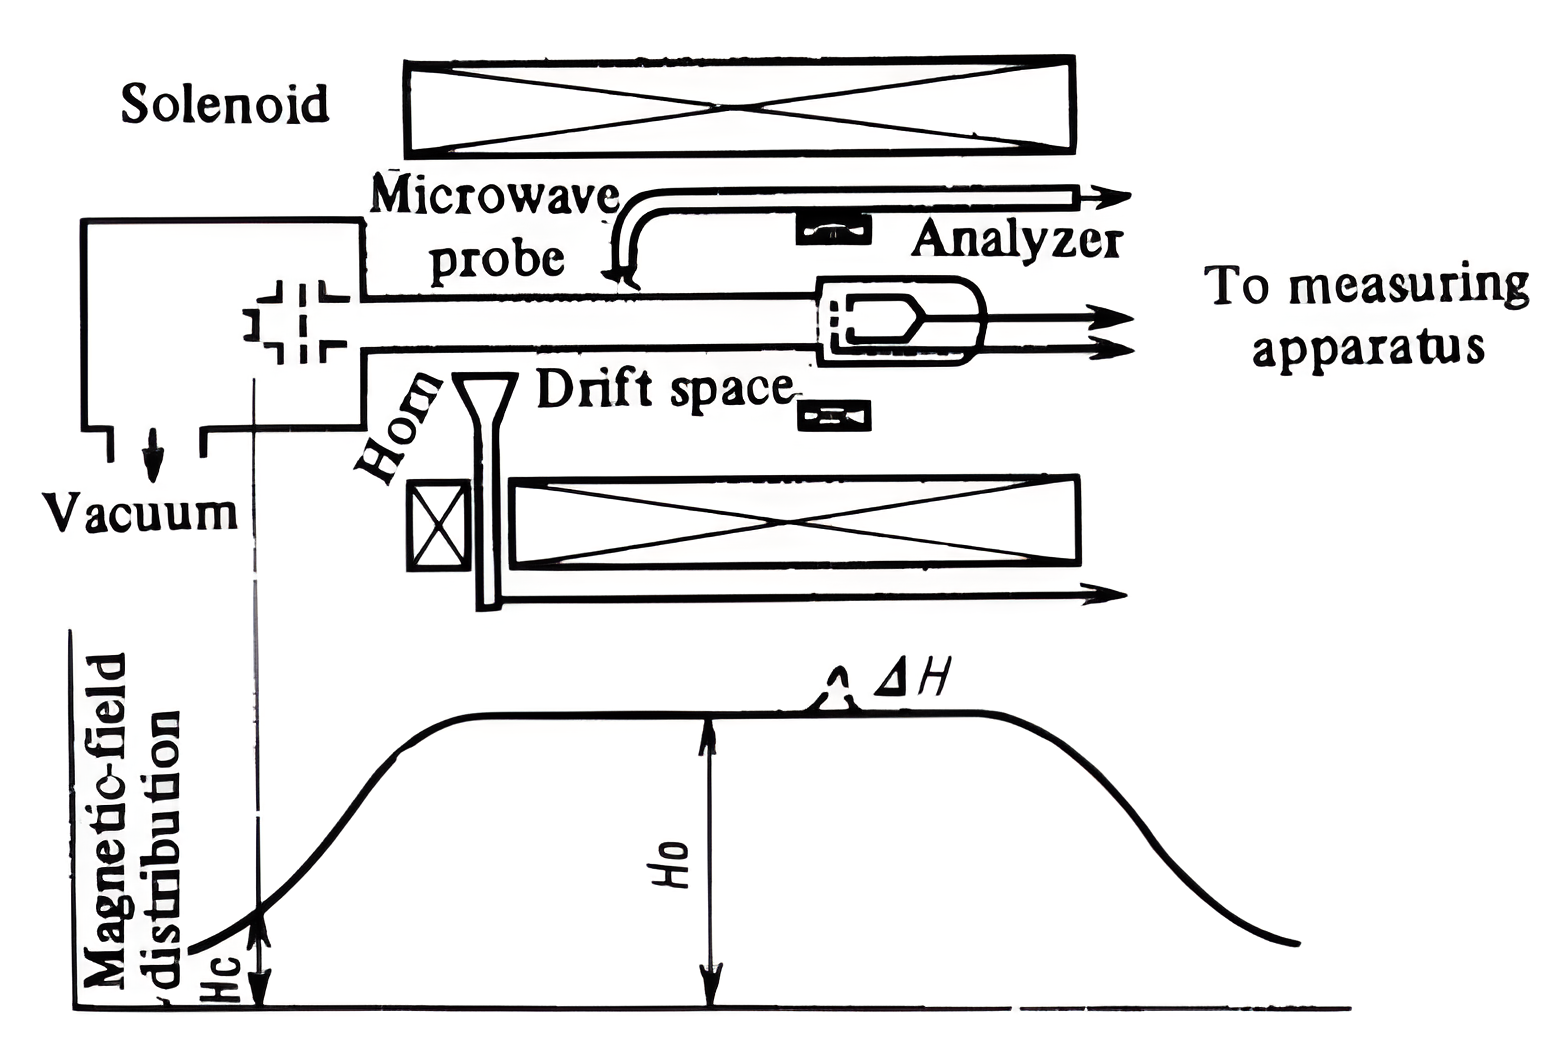
\includegraphics[width=12cm]{image23_1.png}
\caption{\label{fig:EGS1}实验设置}
\end{figure}
针,轴向场线圈以及静电场能量分析仪,静电场能量分析仪由偏压为$U_r$的栅网和用于产生磁镜的线圈构成。\autoref{fig:EGS1}下图表示真空放电管中由轴向场线圈和磁镜线圈构成的总磁场强度分布。静电场能量分析可用于获得束等离子体轴向速度分布函数和轴向速度在$v_∥$和$v_∥+dv_∥$区间具有的横向平均能量。根据不同的$h=ΔH/H_0 $曲线可以测得电子轴向速度$v_∥$对应的横向运动的平均能量为
\begin{equation}
\bar{W}_{\perp}\left(v_{\|}\right)=\frac{\int W_{\perp} f\left(v_{\|}, v_{\perp}\right) d v_{\perp}}{\int f\left(v_{\|}, v_{\perp}\right) d v_{\perp}}=\left.\frac{\frac{\partial I}{\partial h}}{\frac{\partial I}{\partial U_{r}}}\right|_{h \rightarrow 0}
\end{equation}
其中I 表示延迟电流。

实验结果表明,当放电真空管保持良好的真空条件时$(p=10^{-6}mm Hg)$时,电子束分布基本保持在初始速度$v_0$附近,如\autoref{fig:EGS2}(后图)所示,垂直能量基本不超过60eV,极小部分由于磁场不均匀性导致垂直能量达到300eV。当放电真空管残余气体压强增加时,管中等离子体产生双流不稳定性,此时会激发出$\omega< \omega_p$的纵波,从结果来看,这种纵波最终会导致分布函数拉平(\autoref{fig:EGS2}中间),束电子横向最大能量进一步升高到450eV,而拉平分布函数的极有可能是朗道阻尼机制。当放电真空管残余气体压强继续增加到$2.1\times10^{-3}mm Hg$(\autoref{fig:EGS2}前图),电子平行磁场方向能量跳跃式散射到垂直磁场方向,伴随着处在电子回旋频率$ω_{ce}$和等离子体上杂化频率$\sqrt{ω_p^2+ω_{ce}^2}$区间的微波信号产生,且微波极化方向垂直于轴向磁场方向。最终横向能量最大增加到$1500eV$,大部分横向能量达到$500eV$,该现象为反常多普勒效应提供了直接实验证据。
\begin{figure}[ht]
\centering
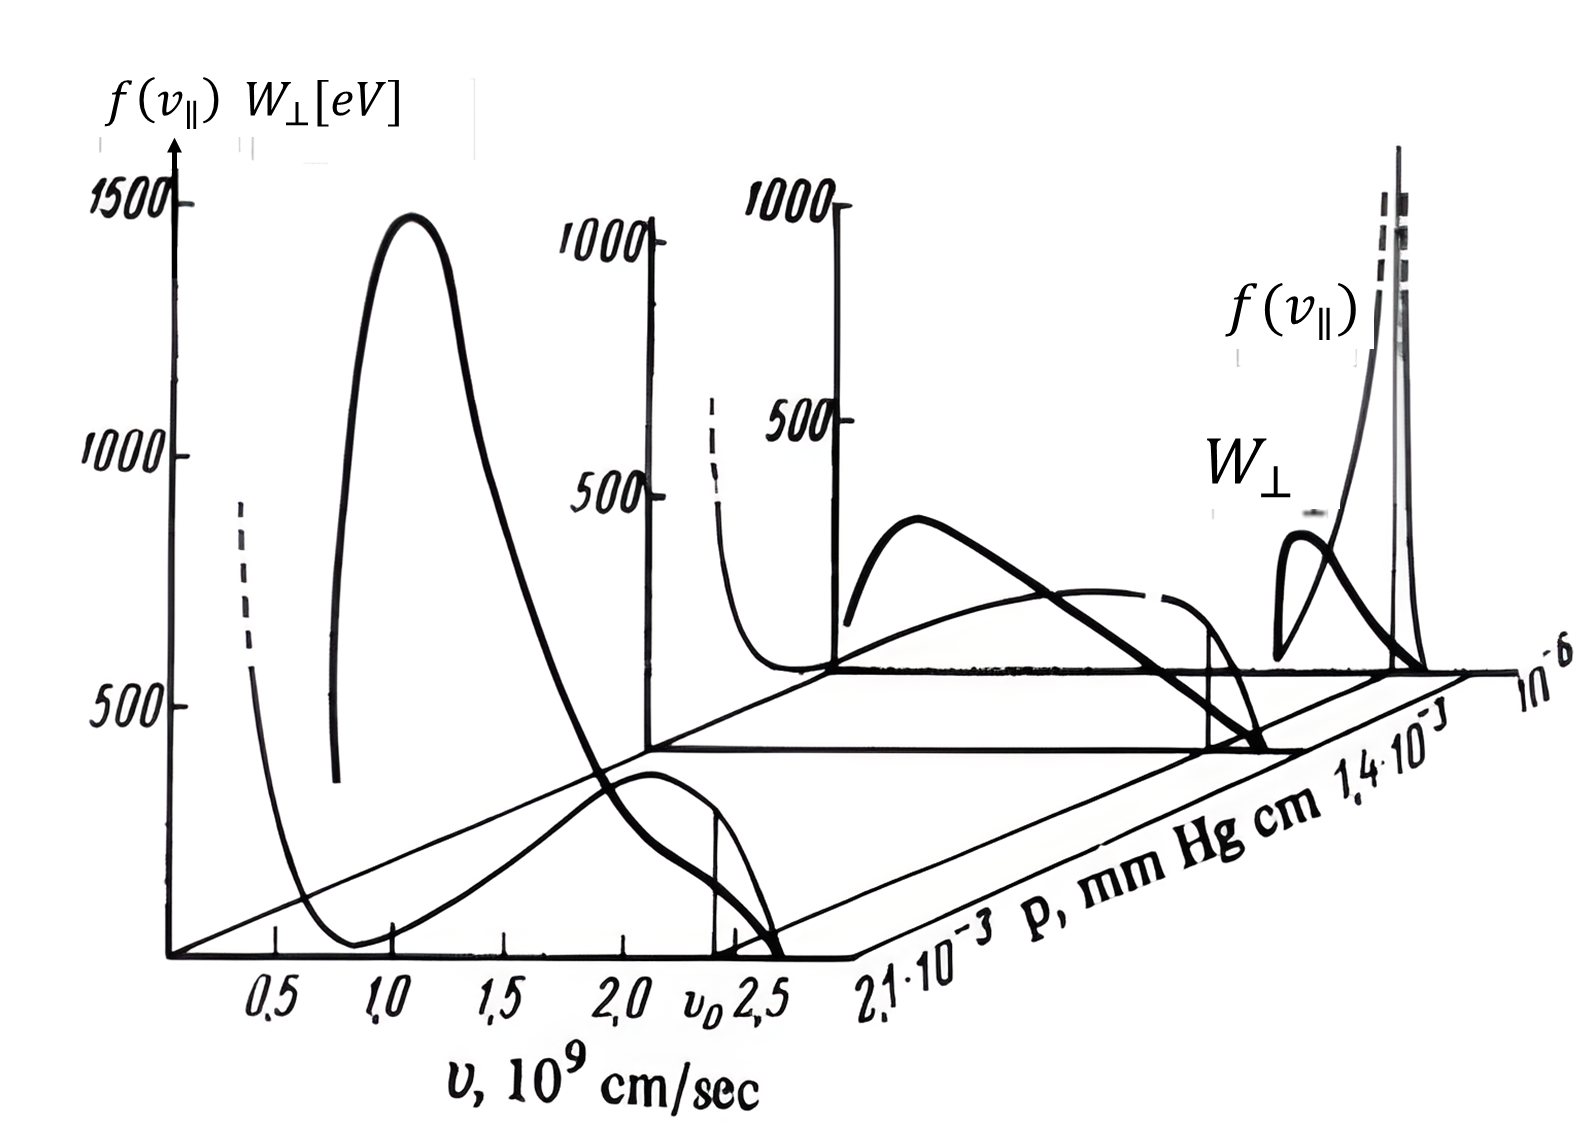
\includegraphics[width=12cm]{image24_1.png}
\caption{\label{fig:EGS2}轴向速度分布函数$f(v_{||})$(细线)和横向平均能量$W_⊥$(粗线);$v_0$表示束电子初始速度\cite{RN786}}
\end{figure}
\par
1976年D.A.Boyd在ATC首次发现电子回旋辐射step结构\cite{RN725},1979年,H. Knoepfel将D.A.Boyd观测到的step现象归因于反常多普勒效应\cite{RN1030}。
\par
1984年,F. Santini在Frascati 托卡马克装置低密度放电条件下,验证了低杂波通过反常多普勒效应对逃逸电子能量的影响\cite{RN1866},实验中逃逸电子能量分别通过硬X射线(H-Xray)和光核反应中子探测,其中硬X射线来源于逃逸电子打在限制器上产生的轫致辐射,电子能量只需要大于500keV就能被有效探测,光核反应中子探测用于探测更高能的电子(14MeV-25MeV)和高z材料相互作用产生的高能$γ$射线和原子核相互作用诱导原子核放出中子,其中等离子体中D-D反应和e-D反应产生的中子可作为背景辐射忽略不计。如\autoref{fig:FST}所示
\begin{figure}[ht]
\centering
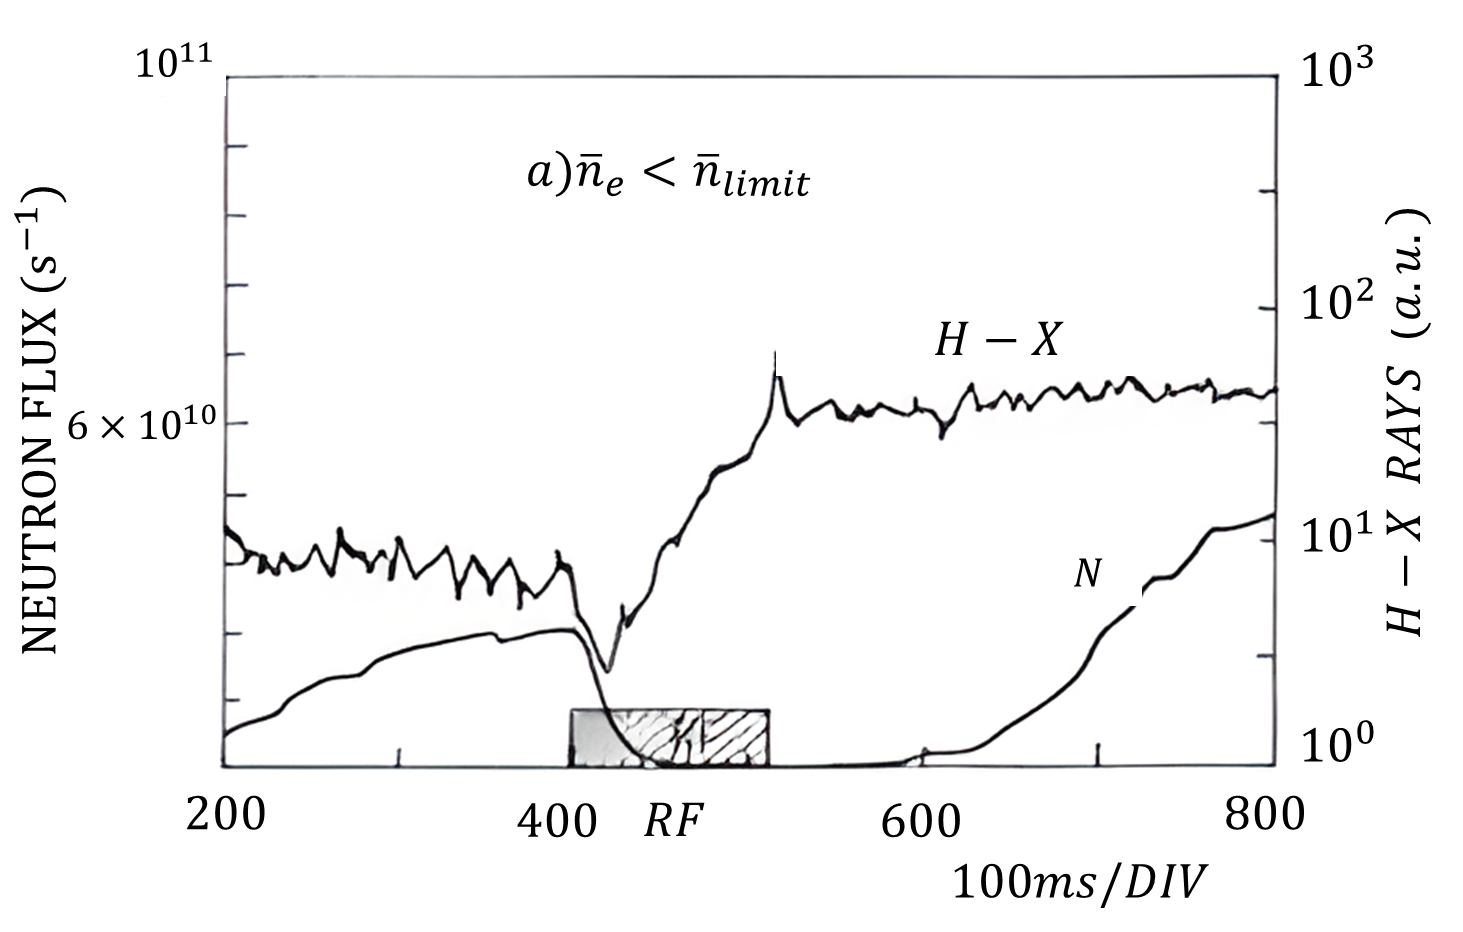
\includegraphics[width=12cm]{image26_1.png}
\caption{\label{fig:FST}氢放电过程光核反应产生的中子和H-X射线的时间演化行为\cite{RN1866}}
\end{figure}
,H-X表示硬X射线,N表示中子辐射,RF表示低杂波注入,从图中可以看出,当RF注入开始时,H-X强度和中子辐射同时开始下降,随后H-X和中子辐射又逐渐上升,这一现象可以通过反常多普勒共振理论和朗道共振解释:当低杂波注入时,高于15MeV高能电子由于和低杂波满足反常多普勒共振条件,高能电子能量向垂直磁场方向散射,逃逸电子动能下降,H-X和中子辐射降低。在低密度条件下,低杂波和电子通过朗道共振使电子速度分布函数形成高达300keV高能尾巴,而逃逸电子临界能量远低于300keV,因此这些电子在环电场驱动下逐渐形成高能逃逸电子,最后导致HX和中子辐射再次上升。

2009年,陈忠勇等人在HT-7托卡马克装置上研究了\autoref{fig:CZY1}step结构产生阈值$ω_{pe}/ω_{ce} $和磁场电流的关系。如\autoref{fig:CZY2}所示,实验结果表明step结构产生阈值和电流存在线性依赖关系,和磁场无关\cite{RN1554}。
\begin{figure}[ht]
\centering
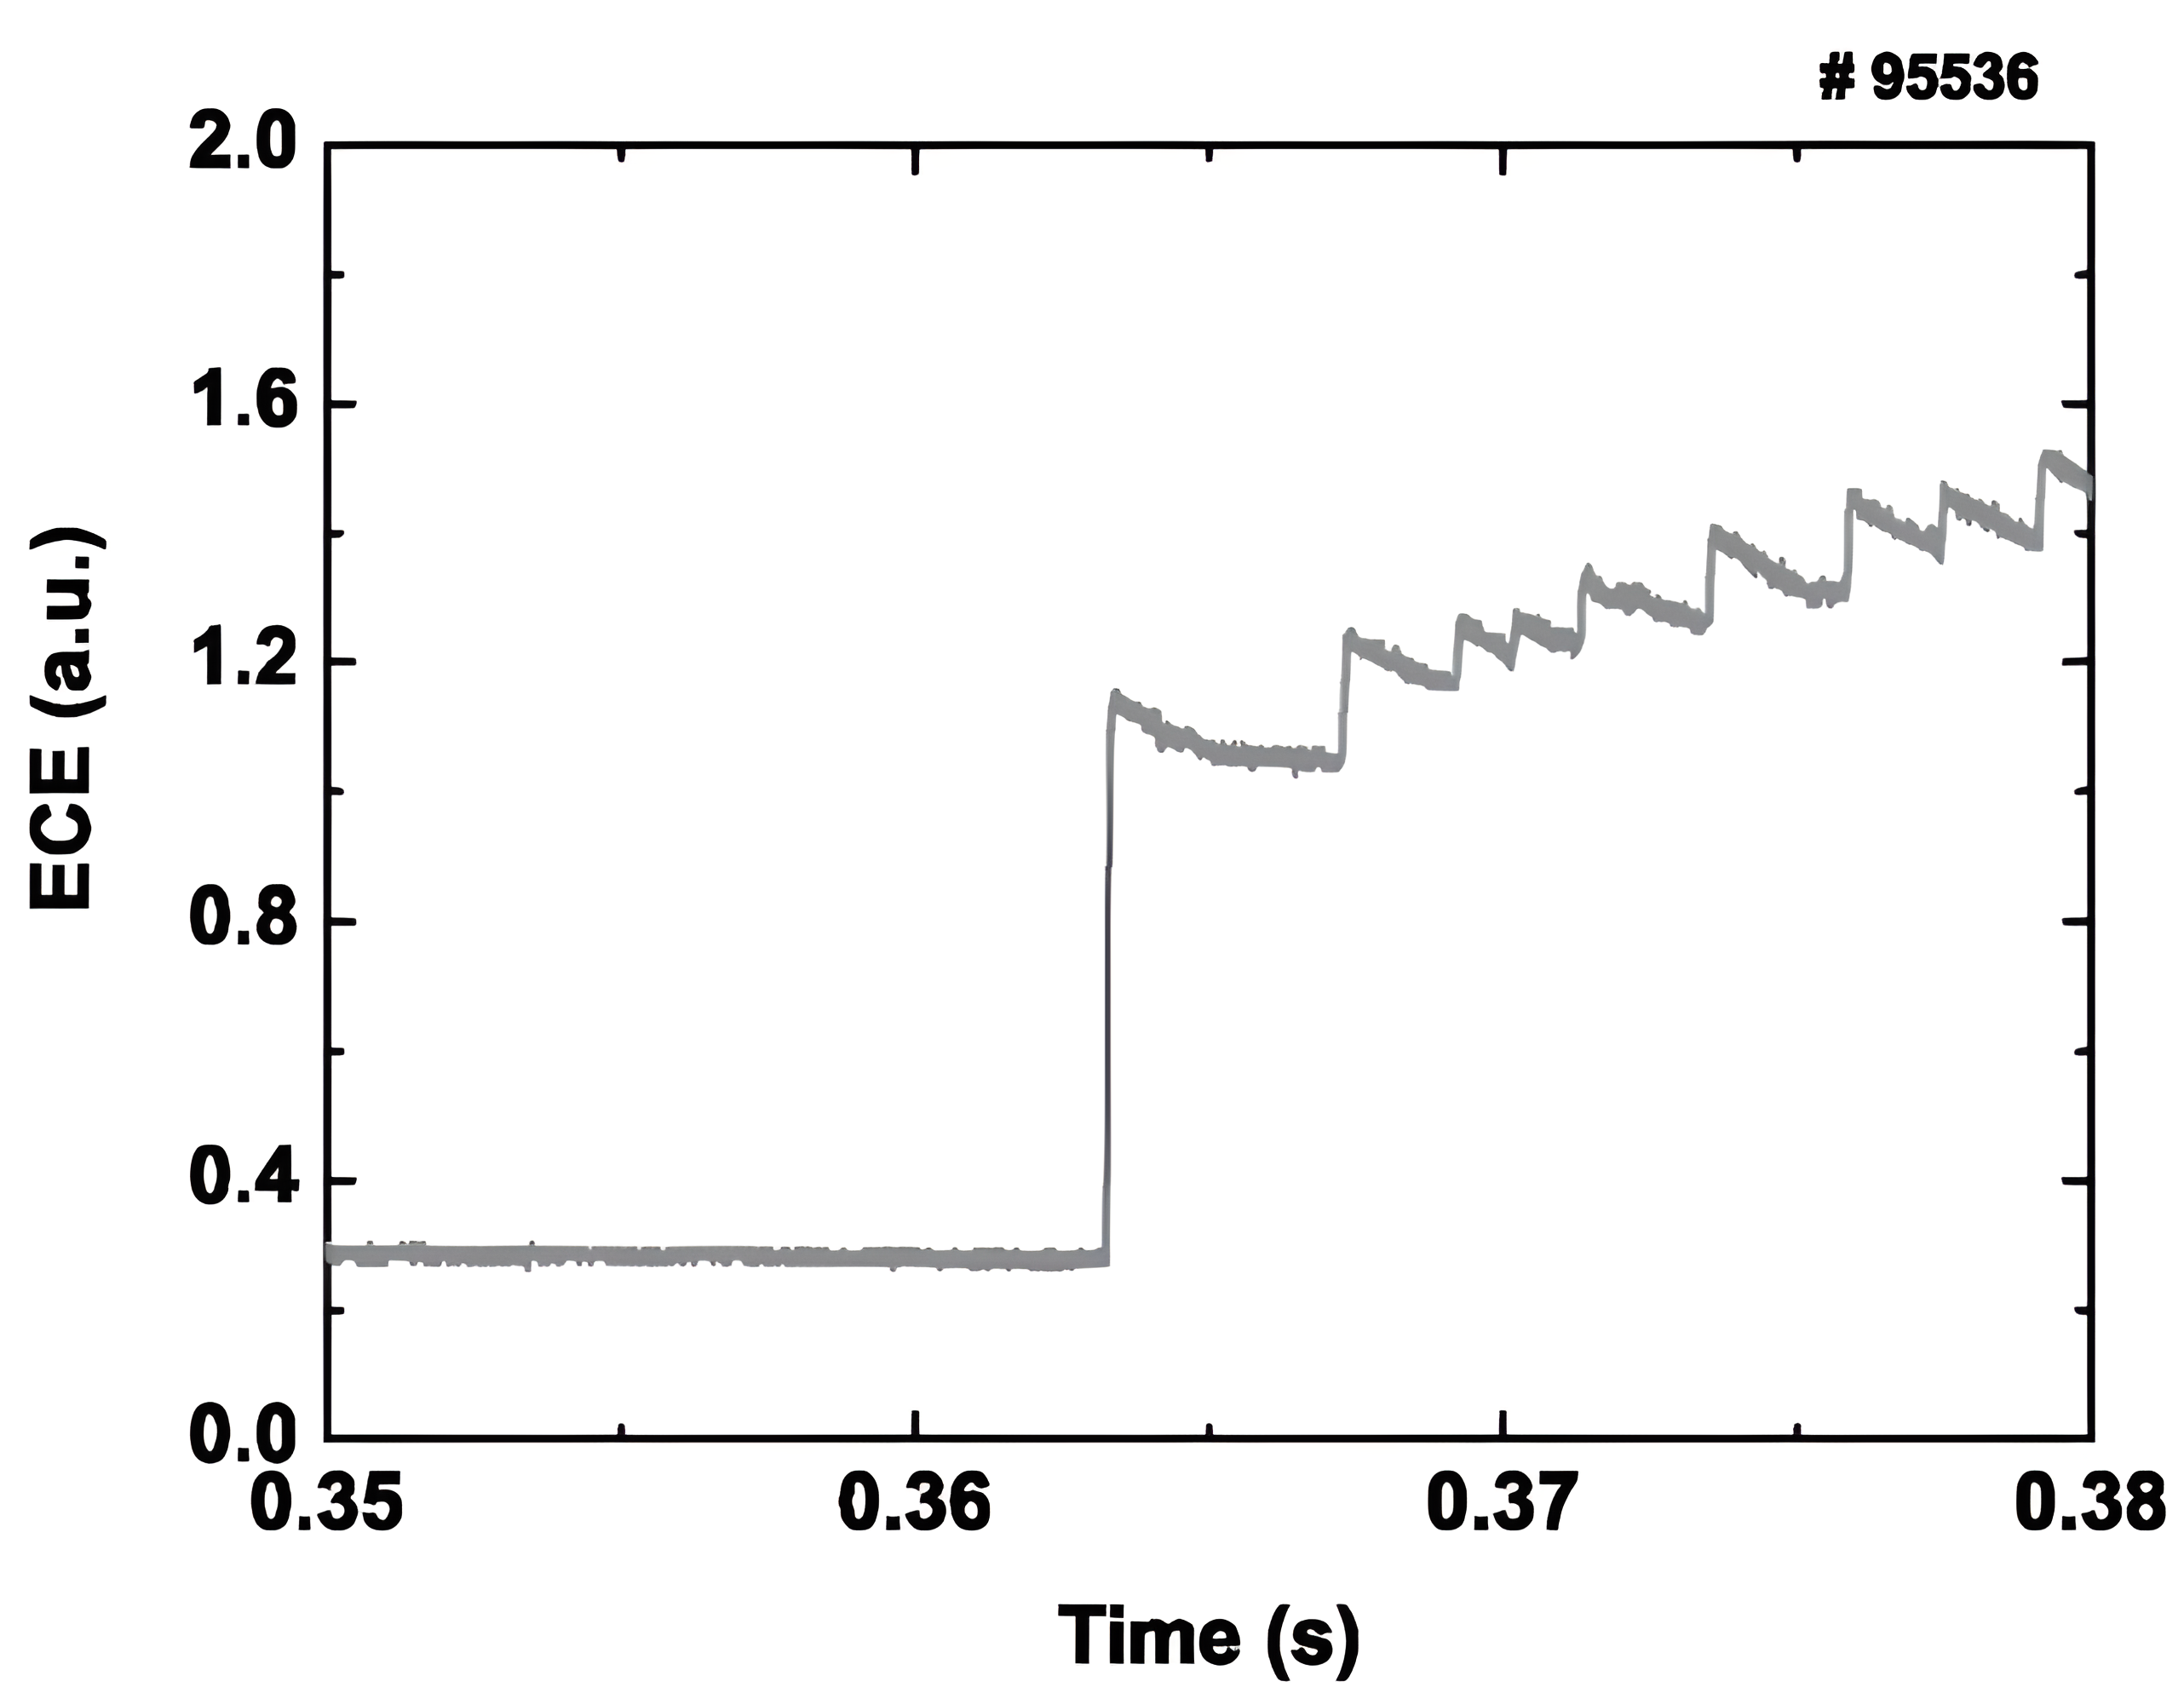
\includegraphics[width=12cm]{image27_1.png}
\caption{\label{fig:CZY1}ECE辐射中step结构\cite{RN1554},纵坐标ECE(a.u.)表示ECE测量信号强度}
\end{figure}
\begin{figure}[ht]
\centering
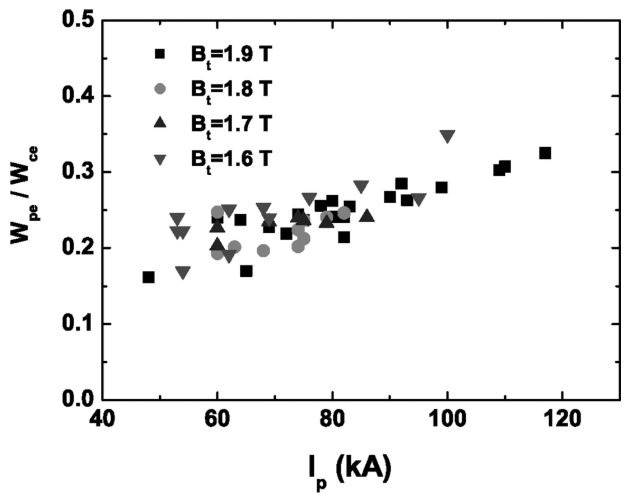
\includegraphics[width=12cm]{image28.png}
\caption{\label{fig:CZY2}不同纵场条件下不稳定性阈值和等离子体电流的依赖关系}
\end{figure}
\par 2010年,卢洪伟等人在EAST装置上研究了ECE信号step结构发生时高能电子的能量转化\cite{RN2102}。如\autoref{fig:LHW1}、\autoref{fig:LHW2}所示,在ECE出现step结构时,通过硬X 射线可以诊断不同能段逃逸电子能量迁移过程。如在$t=2.81$秒,当ECE辐射出现step跳变时(\autoref{fig:LHW1}),通过硬X射线诊断(\autoref{fig:LHW2}a)可以看出能量在1.5-2.0MeV区间逃逸电子迅速下降然后逐渐上升,而能量为9.5-10.0MeV的逃逸电子迅速上升然后缓慢下降。另一方面,\autoref{fig:LHW2}(b)FEB诊断主要用于测量电子垂直方向能量,在2.81秒ECEstep结构产生时50-100keV电子能量迅速上升,而后下降。根据以上现象,论文对该现象解释是当step结构产生时逃逸电子发生散射,其中1.5-2.0MeV逃逸电子散射到50-199keV,而更高能量的逃逸电子则散射到9.5-10.0MeV。
\begin{figure}[ht]
\centering
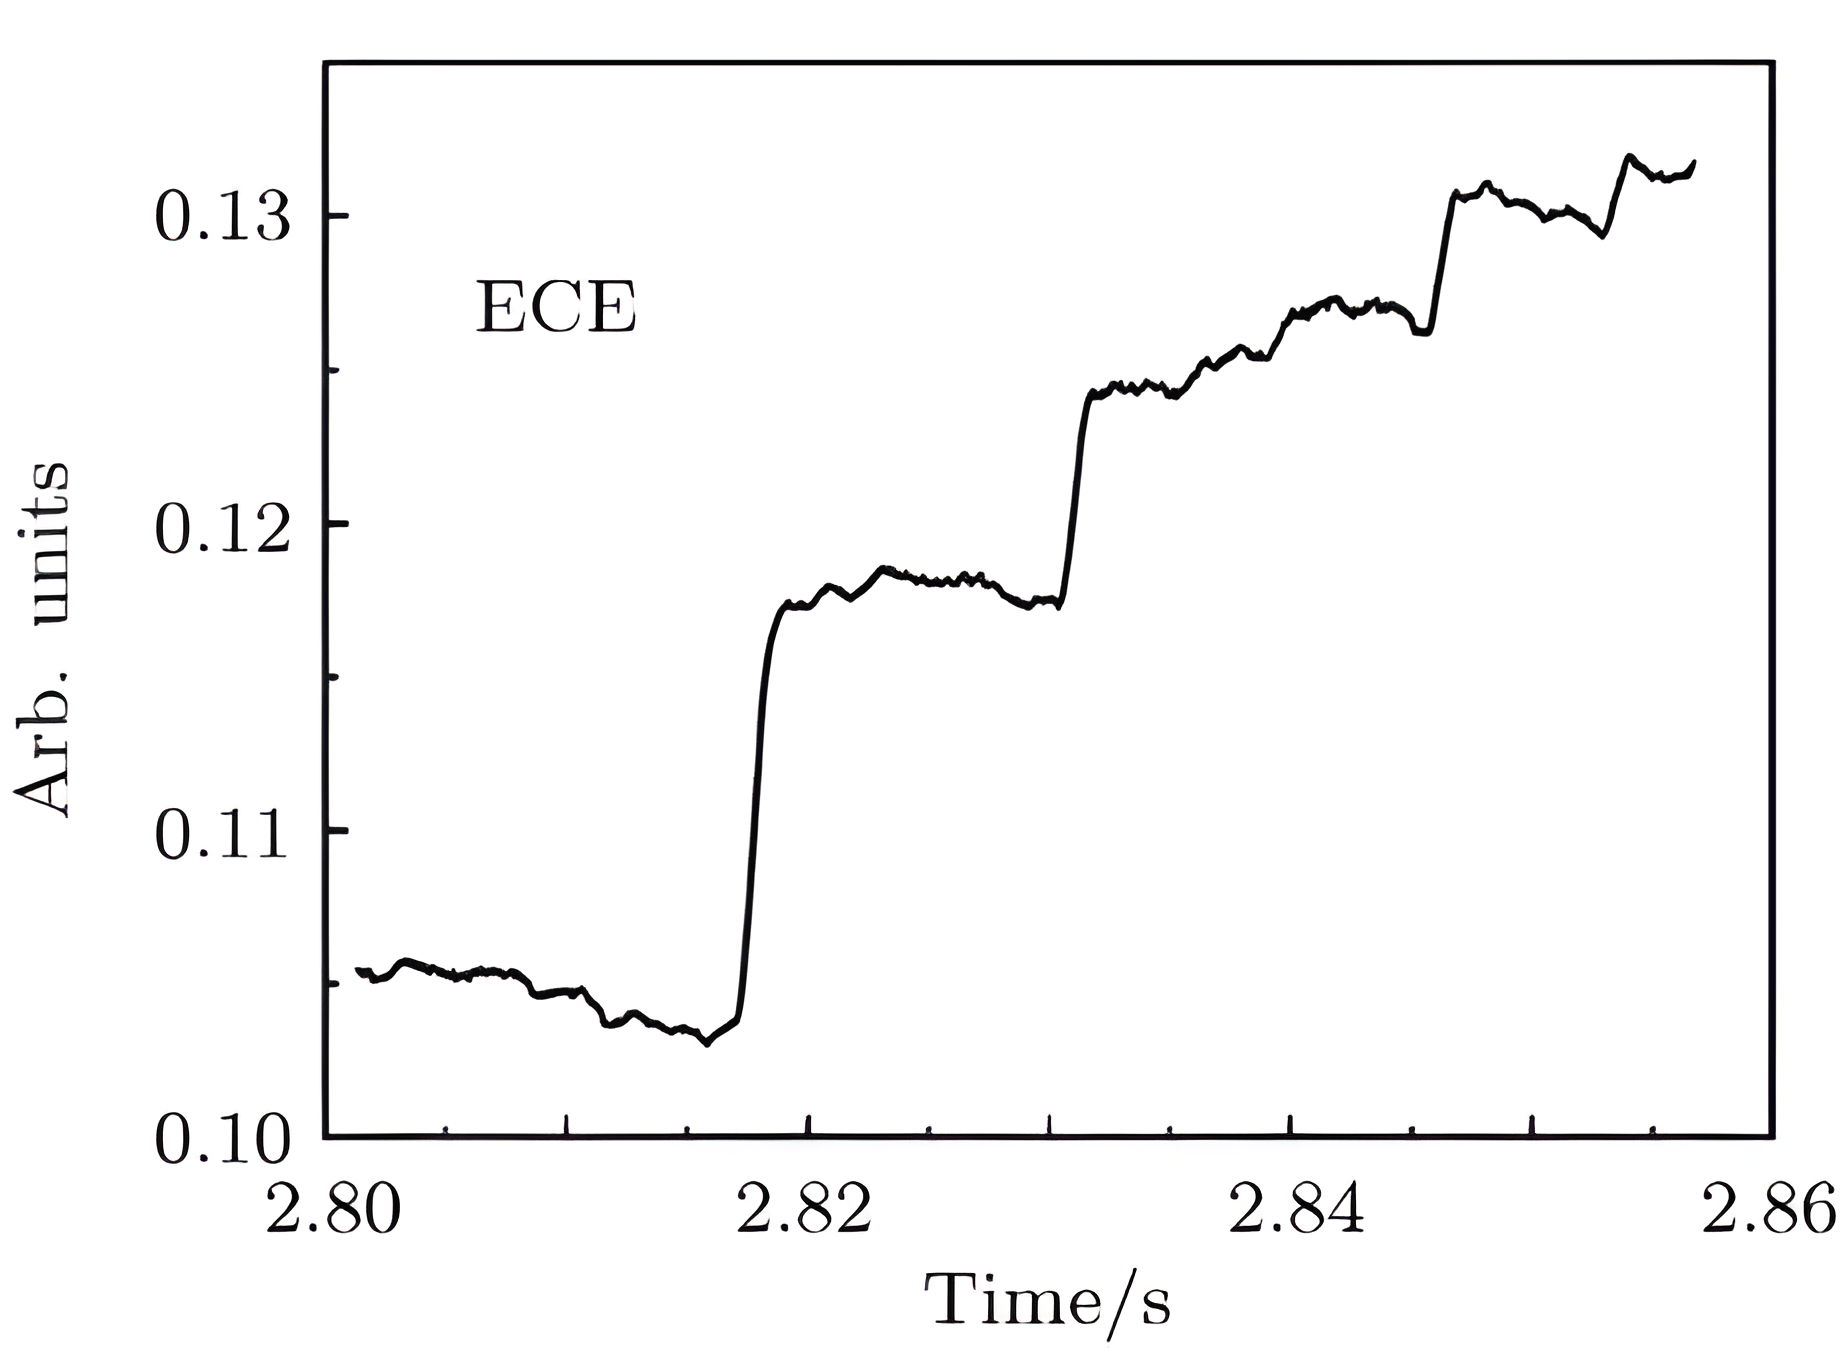
\includegraphics[width=12cm]{image29_1.png}
\caption{\label{fig:LHW1}ECE辐射细节(shot No.12964)\cite{RN2102}}
\end{figure}
\begin{figure}[ht]
\centering
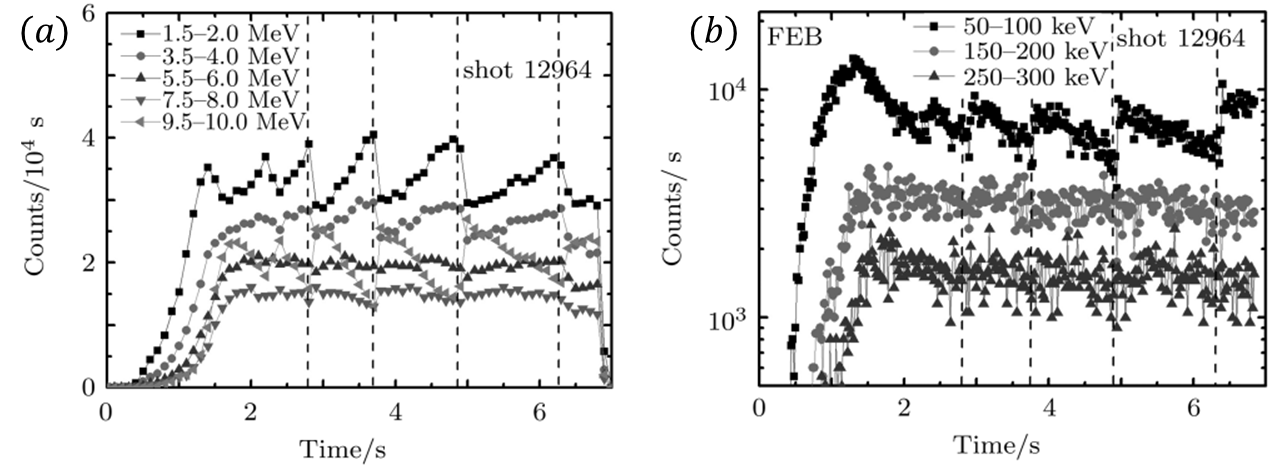
\includegraphics[width=15cm]{image30_1.png}
\caption{\label{fig:LHW2}(a)不同逃逸电子能量范围内通过硬X射线(HX)诊断检测的计数率(shot No.12964)(b)不同逃逸电子能量范围内通过快电子轫致辐射(FEB)诊断检测的计数率(shot No.12964)。图片来自Lu Hong-Wei\cite{RN2102}}
\end{figure}
\par 2015年,S. J. Freethy通过反常多普勒效应解释了在MAST装置上边界局域模(ELM)产生过程中微波辐射尖刺结构\cite{RN1868}(\autoref{fig:SGF})并且用PIC程序模拟电子速度分布函数在多普勒效应作用下随时间的演化(\autoref{fig:SGF2}),证明了反常多普勒效应会使电子速度分布函数趋向于各项同性。
\begin{figure}[ht]
\centering
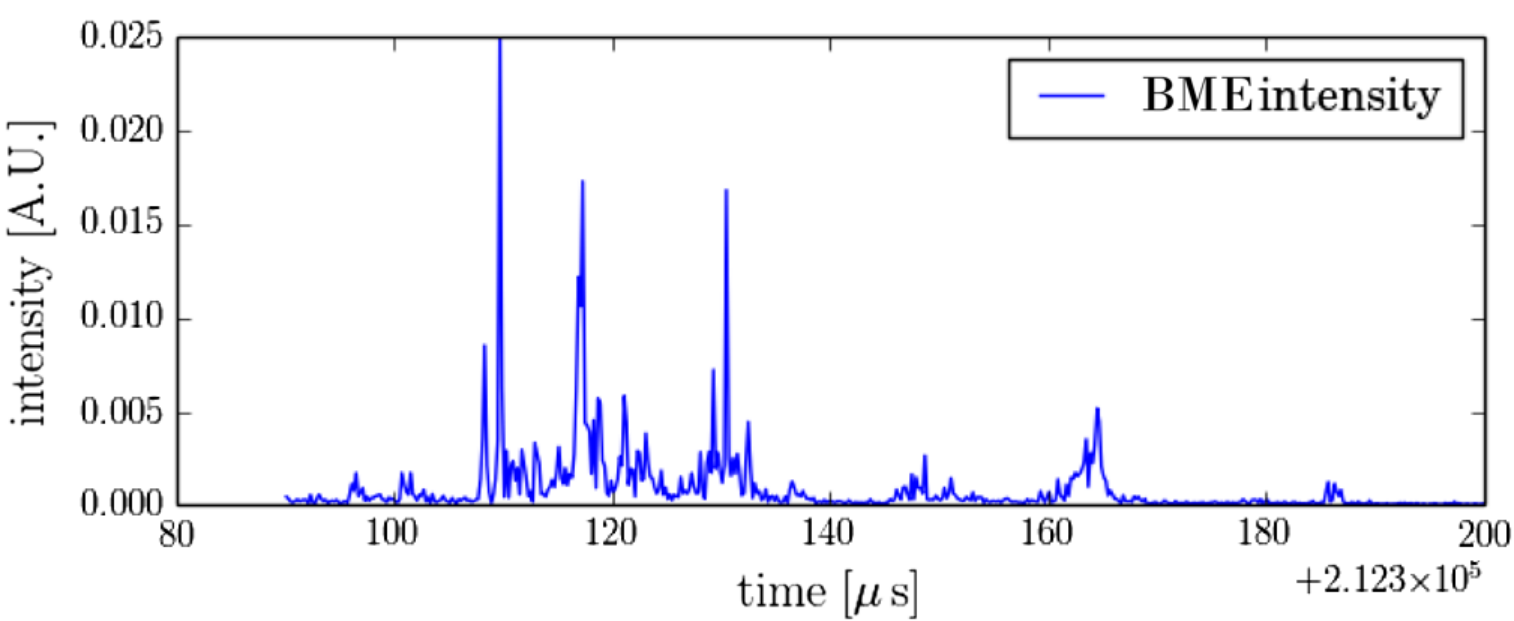
\includegraphics[width=12cm]{image31.png}
\caption{\label{fig:SGF}BMEintensity(Burst Mircowave Emission intensity)微波辐射爆发强度随时间演化\cite{RN1868}}
\end{figure}
\begin{figure}[ht]
\centering
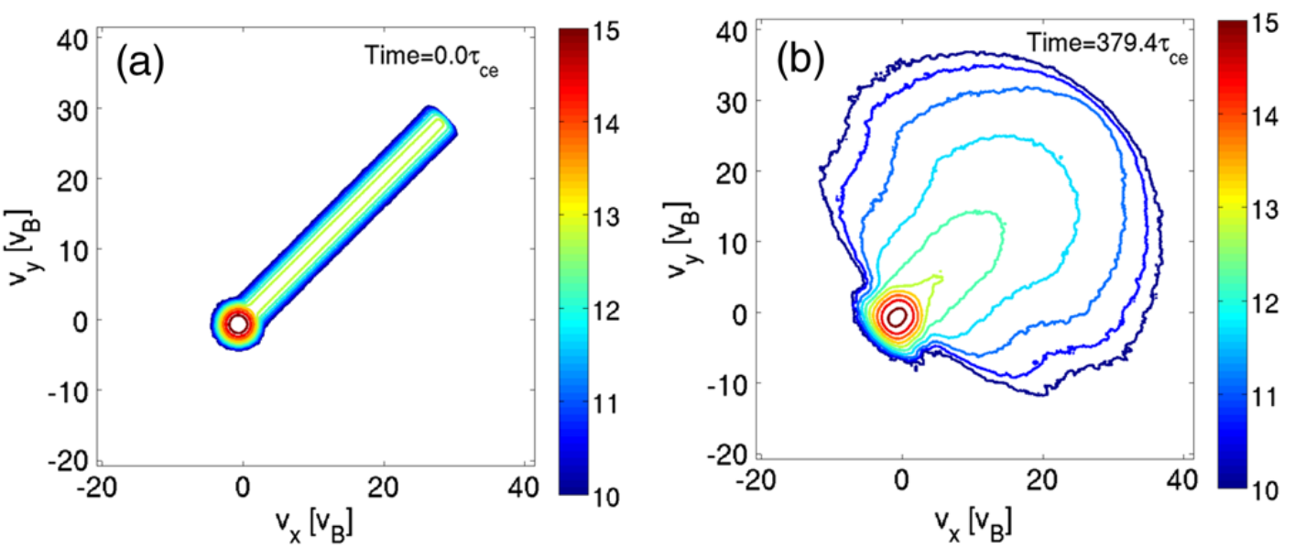
\includegraphics[width=12cm]{image32.png}
\caption{\label{fig:SGF2}PIC模拟逃逸电子分布演化(a)初始电子速度分布(b)末态电子速度分布\cite{RN1868}}
\end{figure}

\begin{figure}[ht]
\centering
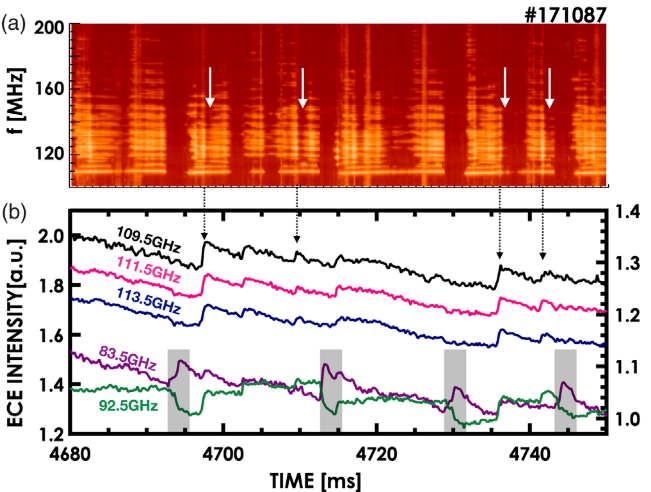
\includegraphics[width=12cm]{image33.png}
\caption{\label{fig:DAS}(a)100-200Mhz磁信号时频谱(b)不同频率的ECE信号,虚线箭头表示哨声波信号的峰值对应的ECE信号\cite{RN975}}
\note{注:图(a)中白色实线表示哨声波信号下降的时刻,图(b)中灰色区域表示n=1的锯齿活动区域}
\end{figure}

\begin{figure}[ht]
\centering
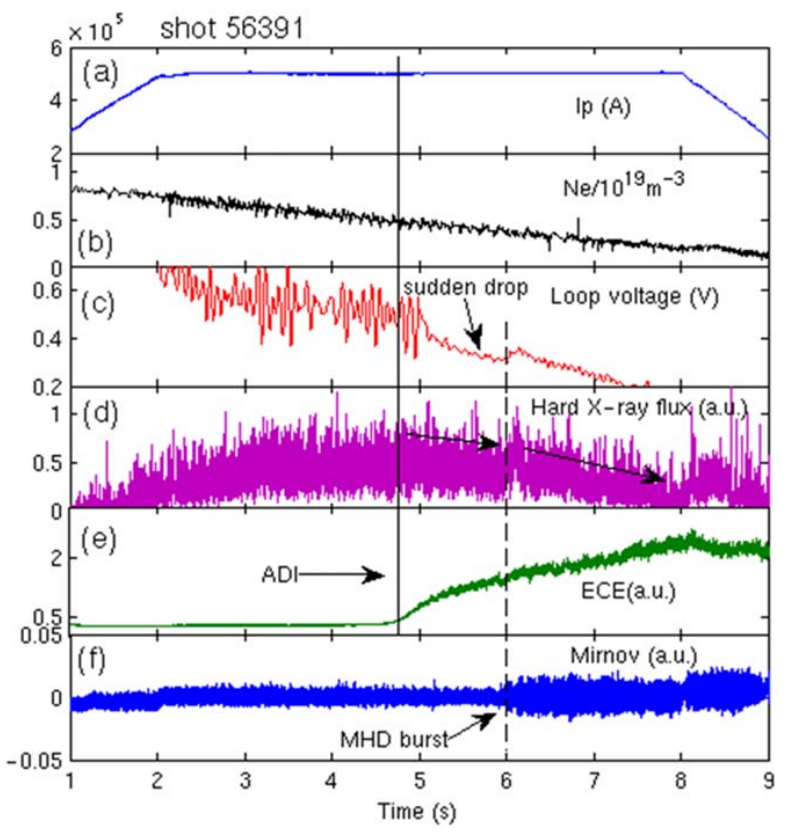
\includegraphics[width=12cm]{image34.png}
\caption{\label{fig:LEZ}EAST\#shot56391:(a)等离子体电流,(b)弦平均电子密度,(c)环电压,(d)硬X射线通量,(e)ECE辐射,(f)Mirnov 信号。垂直实线表示ECE快速爬升起点,垂直虚线表示MHD爆发时间\cite{RN1859}}
\end{figure}
\par 2018年,D. A. Spong等人在DIII-D装置首次观测到逃逸电子激发的哨声波\cite{RN975}, 如\autoref{fig:DAS}所示,其中\autoref{fig:DAS}(a)中高频磁探针测得的多支谐波频率表征高能电子激发的哨声波,\autoref{fig:DAS}(b)表示不同频率电子回旋辐射信号时序图。当哨声波强度达到峰值时,波粒相互作用导致高能电子角度散射,ECE信号迅速上升,随后哨声波强度下降。同年,刘畅利用数值模拟的方法详细分析了逃逸电子激发哨声波的过程并通过反常多普勒效应分析研究了分布函数的动理学演化\cite{RN1815}。虽然\autoref{fig:DAS}(b)电子回旋辐射形状和step结构有点相似,反常多普勒效应的研究取得了很大实验和理论上的进步,但是实际上在哨声波导致的ECE辐射信号波动和ECE的step结构在时间尺度和形状差异上还是非常明显,关于ECE辐射的step结构物理过程仍然没有得到解释。




\begin{figure}[ht]
\centering
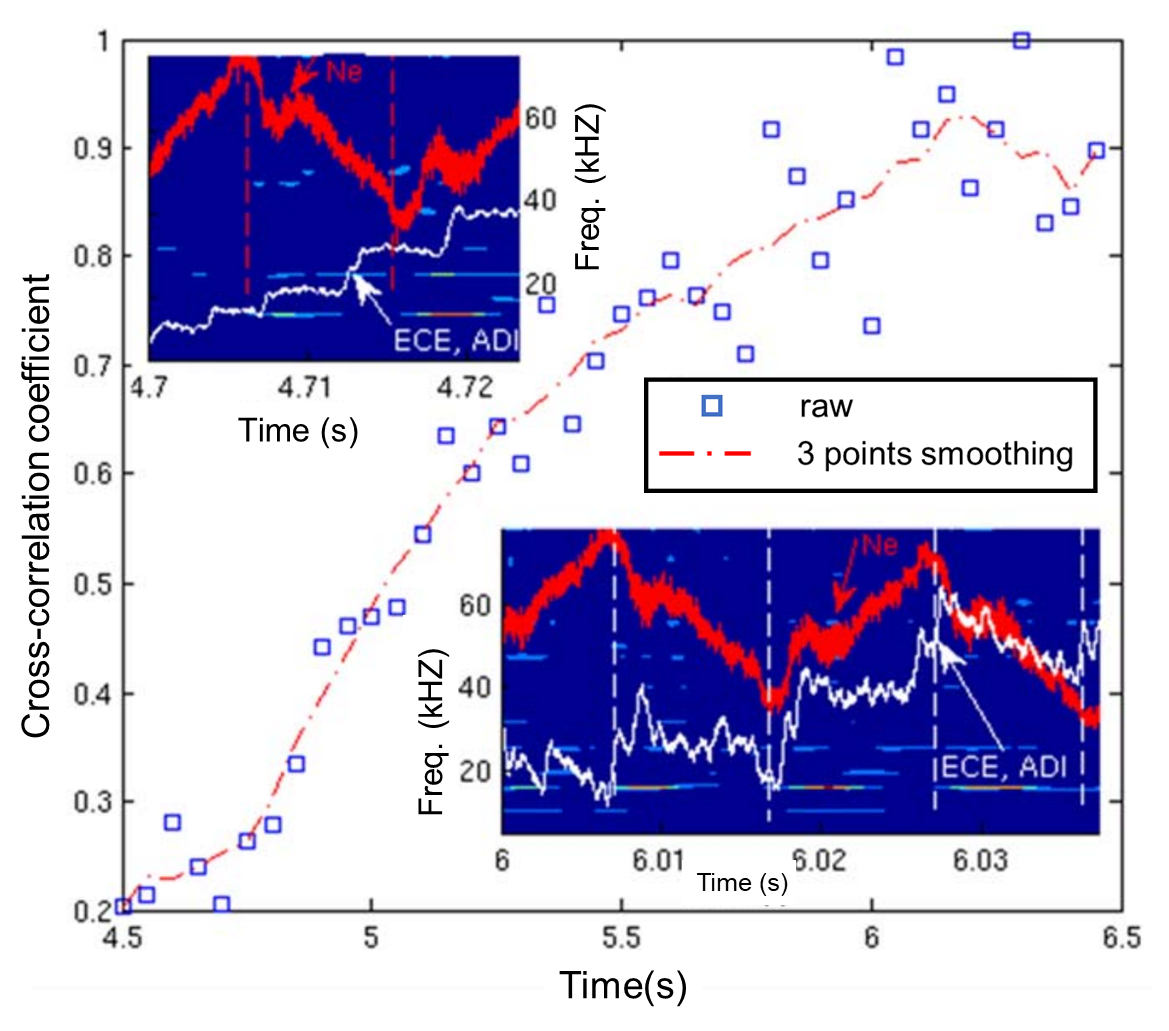
\includegraphics[width=12cm]{image35.png}
\caption{\label{fig:LEZ2}由ADI(反常多普勒不稳定性)导致的ECE信号step结构和密度波动之间的相关系数,左上图和右下图是两张不同时刻的密度波动谱并分别插入了ECE和密度时序信号\cite{RN1859}	}
\end{figure}
 \par 2020年,Li\cite{RN1859}	在EAST装置上通过线性降低等离子体密度观测到了反常多普勒不稳定性 (Anomalous Doppler Instability,ADI)。如\autoref{fig:LEZ}所示,当密度低于$0.5\times10^{19}m^{-3}$时, ECE信
号迅速升高,在4.7s和6s附近放大ECE信号可以看出ECE出现step结构
(\autoref{fig:LEZ2}),在密度波动谱中还可以看到14KHz的频谱信号。文中计算
了在[4.5s-6.5s]区间电子密度波动和ECE信号的互相关系数
\begin{figure}[ht]
\centering
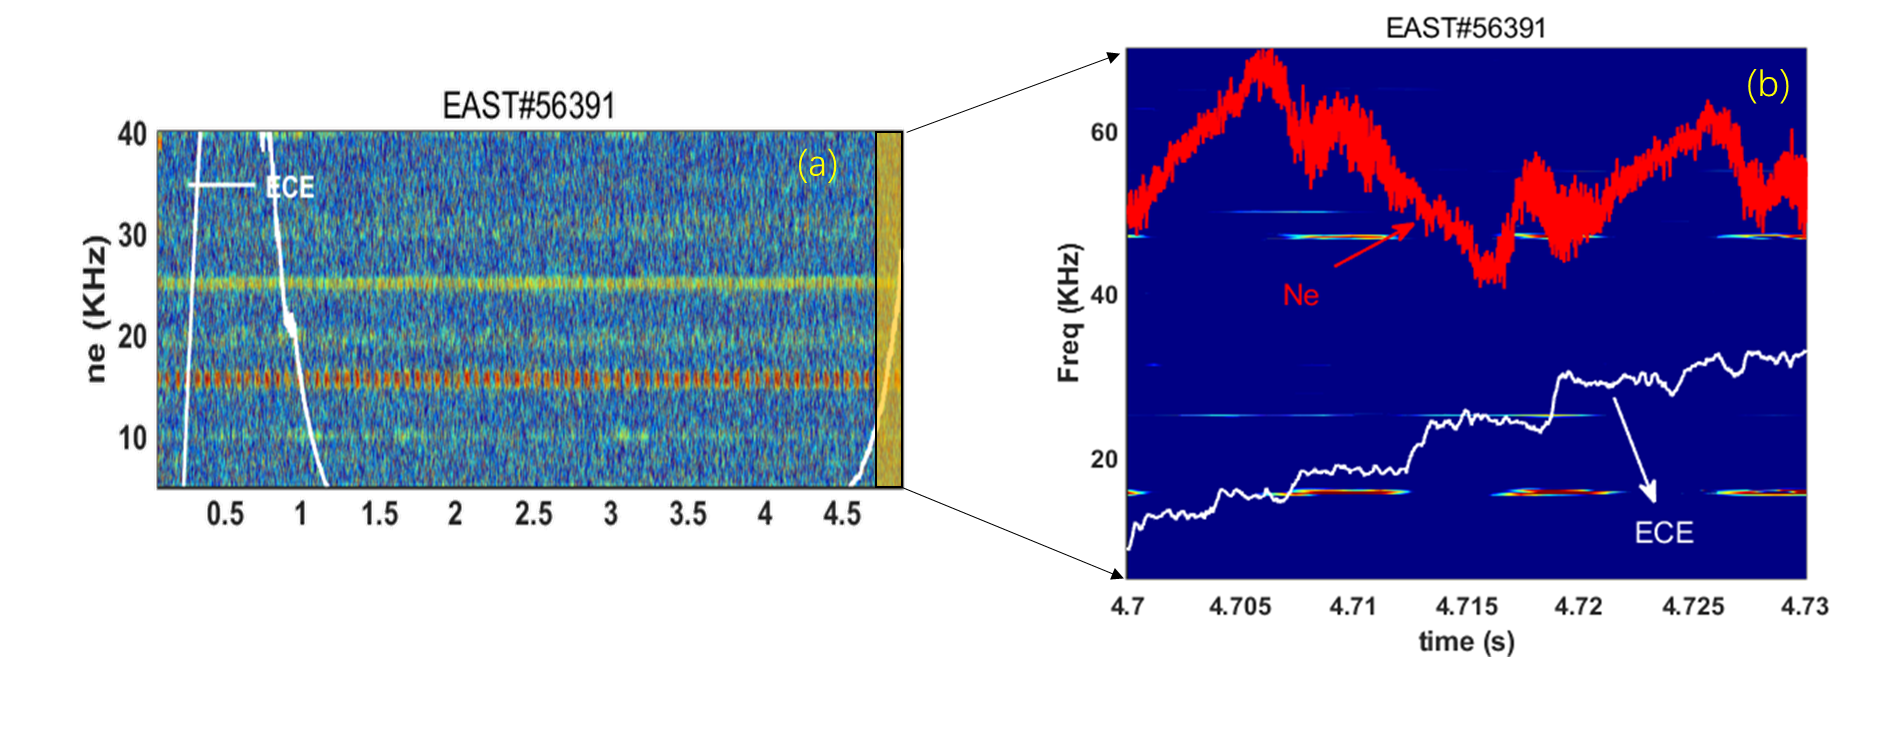
\includegraphics[width=15cm]{image36.png}
\caption{\label{fig:LEZ3}(a)放电期间密度波动谱与电子回旋辐射信号
(b)4.7s~4.73s电子回旋辐射和密度波动谱}
\end{figure}
(\autoref{fig:LEZ2})。如
\autoref{fig:LEZ2}左上角所示,$t\sim4.7s$时密度波动和ECE信号波动相关性较小,此时密度波动发生时间和ECE step上升时间不同步,而
$t\sim6s$时(如\autoref{fig:LEZ2}右下角所示,其中白色虚线
表示密度波动发生时间)密度波动和ECE信号波动具有很强的相关性,此时密度波动发生时
间和ECE step上升时间同步。磁扰动发生在$t\sim6s$之后。根据密度波动和磁扰
动频谱信号,文章指出ECE信号中ADI与磁扰动有关,但没有解释ECE step
结构上升和平台区间的形成机制。比如\autoref{fig:LEZ2}右下角所示密度频
谱(17Khz)出现的时间段内为什么ECE信号是先上升后达到平台?如何解
释\autoref{fig:LEZ2}左上角4.7s ECE step上升时间和密度波动谱出现时间不
一致的现象?这里的实验现象和论证依据还有待进一步检验。实际
上密度谱中周期性出现17KHZ谱线与磁扰动无关,更与ECE信号无关。如
\autoref{fig:LEZ3}(a)所示,这一炮中测量密度的point数据在放电全程一直存
在周期性17KHZ谱线,将其中$4.7s\sim4.73s$放大得到类似\autoref{fig:LEZ2}左上图密度谱的\autoref{fig:LEZ3}(b),所以17KHZ的谱线
是非物理的结果。而ECE信号和密度波动相关性在$t\sim6s$增大是因为出现
了MHD模,相关性增大是理所当然,和电子回旋辐射step结构似乎关系不大。




\par 2021年P Buratti 利用宽带天线在FTU装置上发现ECE辐射的step结构平台区间存在等离子体频率的辐射信号\cite{RN798}。如\autoref{fig:PBT}所示,在ECE信号step结构上升区间存在宽频的辐射爆发,而step结构平台区间存在接近等离子体频率附近的线性谱线,原因有待解释。
\par 综上所述,关于电子回旋辐射信号中出现step结构的实验报道已有很多。虽然大部分工作认为这种结构的产生与反常多普勒效应密切相关,但系统的物理分析一直欠缺。因此我们论文选择电子回旋辐射中得这一step结构开展研究,既不特殊,也不过时。显然电子回旋辐射出现 step 结构与电子速度分布函数的非热成分演化有关,这也是本论文的主要研究方向。
\begin{figure}[ht]
\centering
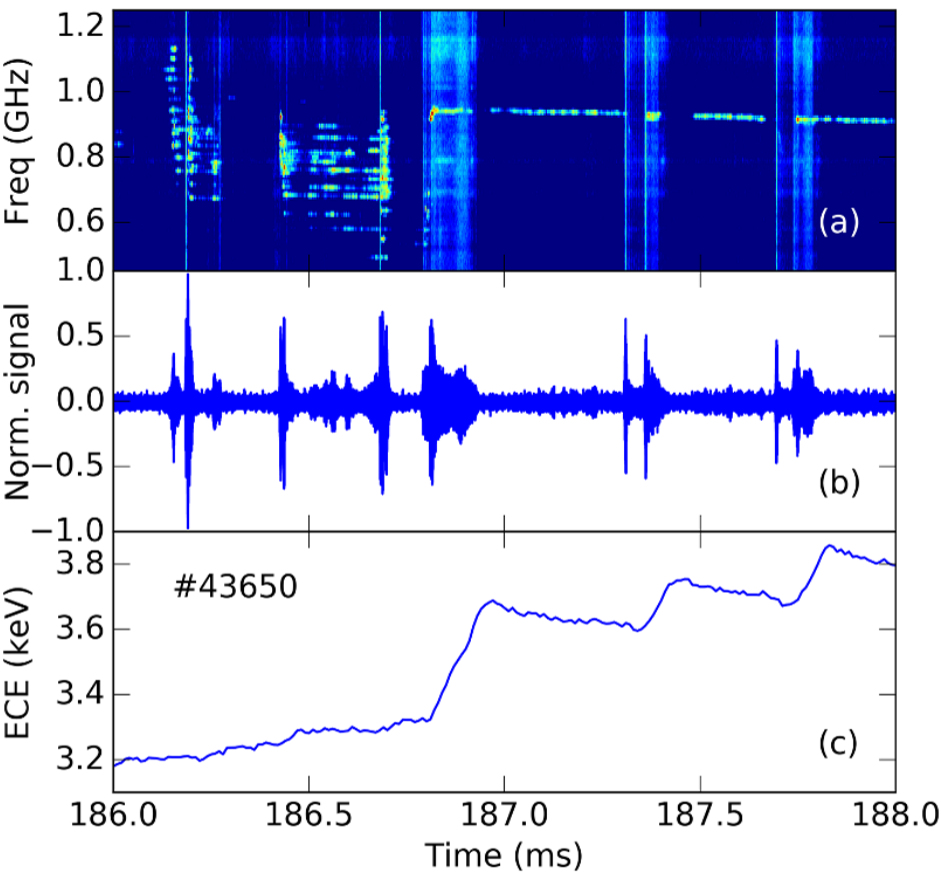
\includegraphics[width=12cm]{image37.png}
\caption{\label{fig:PBT}(a)射频辐射时频图(b)归一化射频原始信号(c)370GHz ECE辐射信号\cite{RN798}}
\end{figure}
%\clearpage
\section{研究意义}
非热化电子作为偏离热分布的一种电子速度分布状态,广泛存在与天体和实验室等离子体中。研究非热化电子产生的物理机制具有重要意义,如太阳耀斑中非热化电子与其磁重联模型之间的关系\cite{RN980},观测地球弓行激波中非热化电子有助于研究电子和哨声波的相互作用\cite{RN981},而测量地球电离层中非热化电子的能量分布又为天体中dynamo current 机制研究提供了重要指导意义\cite{RN981}。在磁约束核聚变装置放电过程中,非热化电子速度分布中的高能尾巴也会影响到磁约束等离子体中的电离、加热、输运以及磁流体稳定性。而未来的ITER装置和CFETR 等聚变堆在高参数运行下,非热化电子的影响也会更加突出\cite{RN1689}。

工欲善其事,必先利其器。电子回旋辐射成像诊断(Electron Cyclotron Emission Imaging , ECEI)是电子回旋辐射的重要诊断工具\cite{RN1020,RN1753,RN2124,RN1044,RN4},肩负着对磁流体动理学的研究任务(MagnetoHydro -Dynamics ,MHD),而且标定后的ECEI还可以测量温度分布\cite{RN1381}。ECEI数据的解读直接关系到最后的成像结果和物理分析,因此对电子回旋辐射的物理本质理解至关重要。通常等离子体需要在满足光学厚和局域热平衡条件下才能正确解读ECEI数据信号。在EAST放电初期电子密度比较低时经常出现电子回旋辐射辐射强度迅速升高,其强度约是平均热辐射强度的一个量级,该信号通常认为是由于低能非热化电子成分导致\cite{RN757}。非热化电子产生后,局域热平衡被破坏,在光学薄的条件下,ECEI信号就不能正确反映等离子体电子温度信息。这样很多时候ECEI数据就因为不满足使用条件而无法用常规方法解读。因此研究非热化电子对正确理解ECEI信号提供了指导意义。通过对ECEI信号产生的本质过程详细分析才有可能对放电过程中ECE辐射信号的各种奇特现象给出合理解释。
\par 鉴于非热化电子重要的物理性质和对电子回旋辐射的影响,各个国家也分别在不同时期开展了电子回旋辐射(ECE)辐射的相关研究。据本人所知,1958年,苏联科学家B.A.TRUBNIKOV首次提出了稀薄等离子体条件下电子回旋辐射和吸收系数的计算方法\cite{RN1003,RN1002};1961年,英国科学家BEKEFI独立提出各项同性速度分布稀薄等离子体电子回旋辐射吸收系数的计算方法\cite{RN1714}并且和1958年B.A.TRUBNIKOV得到的结果相同\cite{RN1003};1976年,C.S.Liu和Y.MOK利用单电子回旋辐射积分方法计算了逃逸电子分布函数的演化对ECE辐射的影响\cite{RN1006};1977年,H. P. Freund, and C. S. Wu提出了高密度等离子体$(ω_{ce}\sim ω_{pe})$辐射计算方法,并给出热平衡条件下各项同性麦克斯韦分布辐射谱的解析结果\cite{RN1007};1983年,M.Bronatici考虑等离子体色散效应,给出热等离子体吸收系数的计算方法\cite{RN1717};1987年荷兰R.M.J.Sillen开发ECE计算代码NOTEC\cite{RN1009};1992年,美国R.W.Harvey结合WKB射线追迹方法计算了非热化电子分布对ECE的影响\cite{RN1010};1995年,法国D.Vezard计算了少量相对论电子的电子回旋辐射和吸收系数\cite{RN2031};2008年,意大利科学家Figini编写了SPECE程序用于研究非热化电子对ECE的影响\cite{RN1013};2017年,美国普林斯顿大学的石磊博士结合M.Bornatici给出的热电子分布条件下ECE吸收系数公式,给出了热平衡条件下ECE辐射的数值合成诊断\cite{RN1014};2019年,德国SeVerin Sebastian Denk为了研究ASDEX Upgrade 托卡马克上的非热化电子编写了Erad code\cite{RN1014}。
\par 国内相关研究开展不多。1993年,丁玄同利用电子回旋辐射模型,结合极化型迈克尔逊干涉仪,分析了HL-1托卡马克中各放电阶段电子回旋辐射谱的特点\cite{RN1017}。其模型中只考虑了电子回旋辐射效应,没有考虑到电子回旋辐射在路径中的吸收效应,因此在放电初期和放电末期时,等离子体密度比较低,吸收效应不显著,模型结果和实验比较定性吻合,即一次回旋辐射强度最大,二次三次回旋频率依次减小。当放电处于密度较高的平顶段时,由于吸收效应不可忽略,辐射谱具有热辐射谱特征,因此模型得不到和实验一致的频谱。2018年中国科学院等离子体研究所ECE诊断组借助意大利SPECE程序分别研究了欧姆加热和LHW加热下ECE谱特征,并根据信号谱的形状拟合出高能尾巴的电子能量\cite{RN2115};2019年该组进一步利用SPECE程序分析了低杂波加热对ECE信号位置对应关系的影响\cite{RN1402}。

随着托卡马克放电参数不断提高, ECE诊断也会面临新的挑战。根据TFTR和JET的放电参数\cite{RN1019},当电子温度升高时,TS测量数据和ECE测量数据的偏差也会逐渐增大,这是由于电子速度在0.75$u_{th}≤u≤1.5u_{th}$区间上分布函数偏离麦氏分布。如\autoref{fig:img38}所示,导致电子在热速度附近形成非麦氏分布的原因目前还没有物理模型能够解释,除非存在很强的驱动机制,比如波粒共振打破了电子热速度分布。根据TFTR和JET观测到的参数外推ITER,当等离子体芯部温度达到20$\sim$40keV时,$T_{ECE}$和$T_{TS}$的差别将会达到50\%。所以中国发展一套数值合成诊断用于分析ECEI数据已是大势所趋。通过建立非热化电子分布和电子回旋辐射强度的关联,我们可以在非热化电子动理学演化过程中分析电子回旋辐射强度的变化。结合电子回旋辐射诊断观测到的现象,我们就可以探究实验过程中可能发生的物理过程,让我们对未来的物理诊断信号的分析具有了更加全面的认识。
\begin{figure}[ht]
\centering
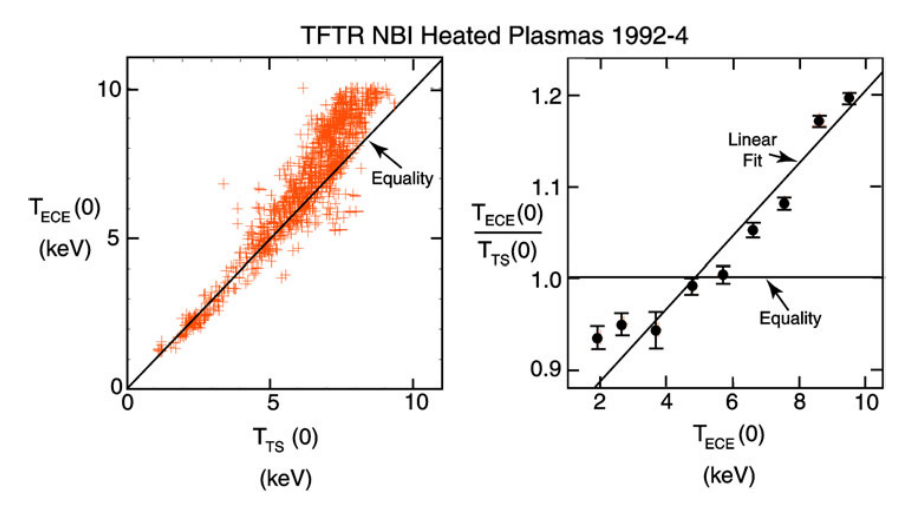
\includegraphics[width=12cm]{image38.png}
\caption{\label{fig:img38}TFTR芯部电子温度中ECE和TS测量结果,随着温度上升,测量分歧也越来越大,电子温度达到10keV时,Ts和ECE测量结果偏差达到20\%}
\end{figure}
\section{论文内容介绍}
在绪论中,本文从托卡马克放电过程入手,引出了非热化电子的产生机制,并探讨了其垂直方向温度来源与反常多普勒效应之间的联系。反常多普勒效应通常用于解释电子回旋辐射中出现的台阶状结构。然而,尽管相关研究已持续了半个多世纪,关于台阶结构的许多关键问题仍未得到解决,例如:导致电子回旋辐射出现台阶结构的具体动理学过程是什么?除了这些独特的物理现象,托卡马克放电还伴随破裂风险。当破裂发生时,会瞬间产生大量逃逸电子,其能量可达数十 MeV,这些高能电子在强电场加速下撞击第一壁或偏滤器,可能对装置造成严重损伤。然而,逃逸电子的动理学过程至今仍未完全掌握,而要避免其对装置的破坏,必须深入理解其产生机制及演化规律。

本论文的研究方法以动理学数值模拟为核心,通过求解电子速度分布的演化,计算电子回旋辐射强度与速度分布之间的关系,从而模拟不同放电条件下电子回旋辐射的演化特征。论文的章节安排如下:第二章介绍电子回旋辐射诊断系统以及观测到的反常辐射信号;第三章综述非热化电子的理论与实验研究,归纳前人的研究经验和方法,为后续的数值模拟奠定理论基础;第四章重点描述电子回旋辐射能量输运过程的计算模型,包括发射率、吸收率及传播路径等问题;第五章介绍非热化电子动理学模型的数值计算方法,并进一步研究单电子运动过程中的反常多普勒效应,详细分析其受力机理,并提出利用电磁波抑制逃逸电子的潜在方案;第六章结合实验研究非热化电子速度分布的演化,并利用动理学模型对托卡马克放电过程中观测到的电子回旋辐射变化进行深入分析。最后,第七章给出全文的总结与未来研究展望。
%
%Lorem ipsum dolor sit amet, consectetur adipiscing elit, sed do eiusmod tempor
%incididunt ut labore et dolore magna aliqua.
%\footnote{Ut enim ad minim veniam, quis nostrud exercitation ullamco laboris
%  nisi ut aliquip ex ea commodo consequat.
%  Duis aute irure dolor in reprehenderit in voluptate velit esse cillum dolore
%  eu fugiat nulla pariatur.}

% !TeX root = ../main.tex

\chapter{电子回旋辐射与反常辐射}
\section*{引言}
本节首先阐明了电子回旋辐射成像诊断的基本原理,并提出了光学透镜表面优化的方案,为提升信噪比和后续实验研究奠定了理论基础。通过分析放电初期的电子回旋辐射信号,观测到具有前端峰值和台阶状特征的辐射结构。通过与国内外相关实验结果的对比,进一步探讨了反常多普勒效应的背景及其研究现状,为深入研究非热化电子演化过程提供了重要依据。
\section{电子回旋辐射成像诊断及光学优化}
\subsection{电子回旋辐射成像诊断简介}\label{sec:ECEI}
电子回旋辐射成像诊断\cite{RN1020}(Electron cyclotron emission imaging [ECEI] )是二维微波成像系统。ECEI大口径高斯光学透镜能够实现将像面中电子回旋辐射信号投射在物面天线上,实现对像面中温度波动测量。如\autoref{fig:ECEIstru}所示,图中左侧大矩形区域表示EAST装置D型截面,小矩形区域表示ECEI成像区间,红色光束表示接收光路,透镜的功能是实现变焦和场曲调节,使得接收天线能够有效探测到目标空间的辐射信号。天线负责接收等离子体中电子回旋辐射信号并对接收信号通过外差降频传输给后端中频系统,信号在中频经过降频滤波检波后得到的视频信号接入采集卡,通过模数转换变为数字信号,最后通过数据分析即可获得温度涨落分布时间演化图。ECEI具有大尺度高时间空间分辨率的观测优势,通过ECEI可以实现对大尺度MHD行为的直接观察,为研究磁重联过程中丰富的物理提供了有力的诊断工具。\autoref{fig:ECEIimag}展示的是Sawtooth\cite{RN1791}过程中观察到的温度涨落随时间的演化过程,相对于传统的一维电子回旋辐射诊断(ECE)\cite{RN742},ECEI诊断提供了更加丰富直观的物理图像。
\begin{figure}[ht]
  \centering
  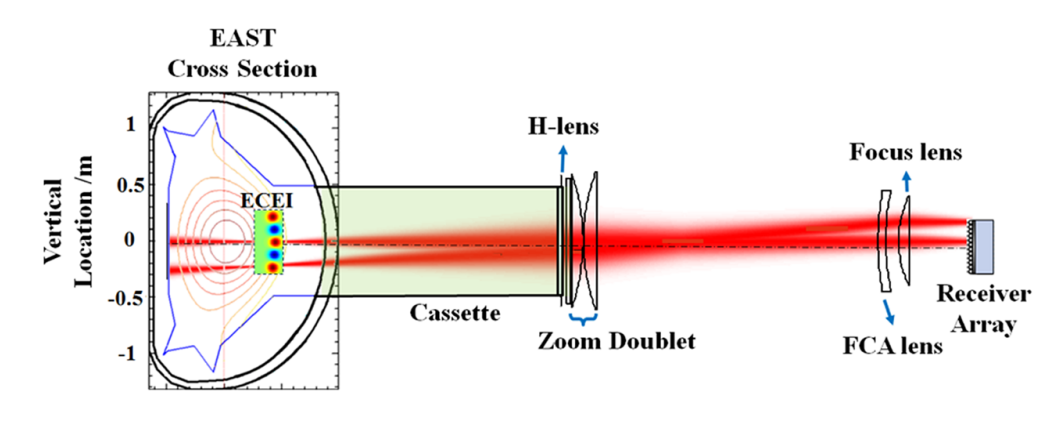
\includegraphics[width=12cm]{image9.png}
  \caption{\label{fig:ECEIstru} ECEI概念图\cite{RN1847},从左至右分别为EAST极向小截面(蓝色区域为ECEI观测范围)、接收透镜、ECEI天线阵列等 }
\end{figure}


\begin{figure}[h]
  \centering
  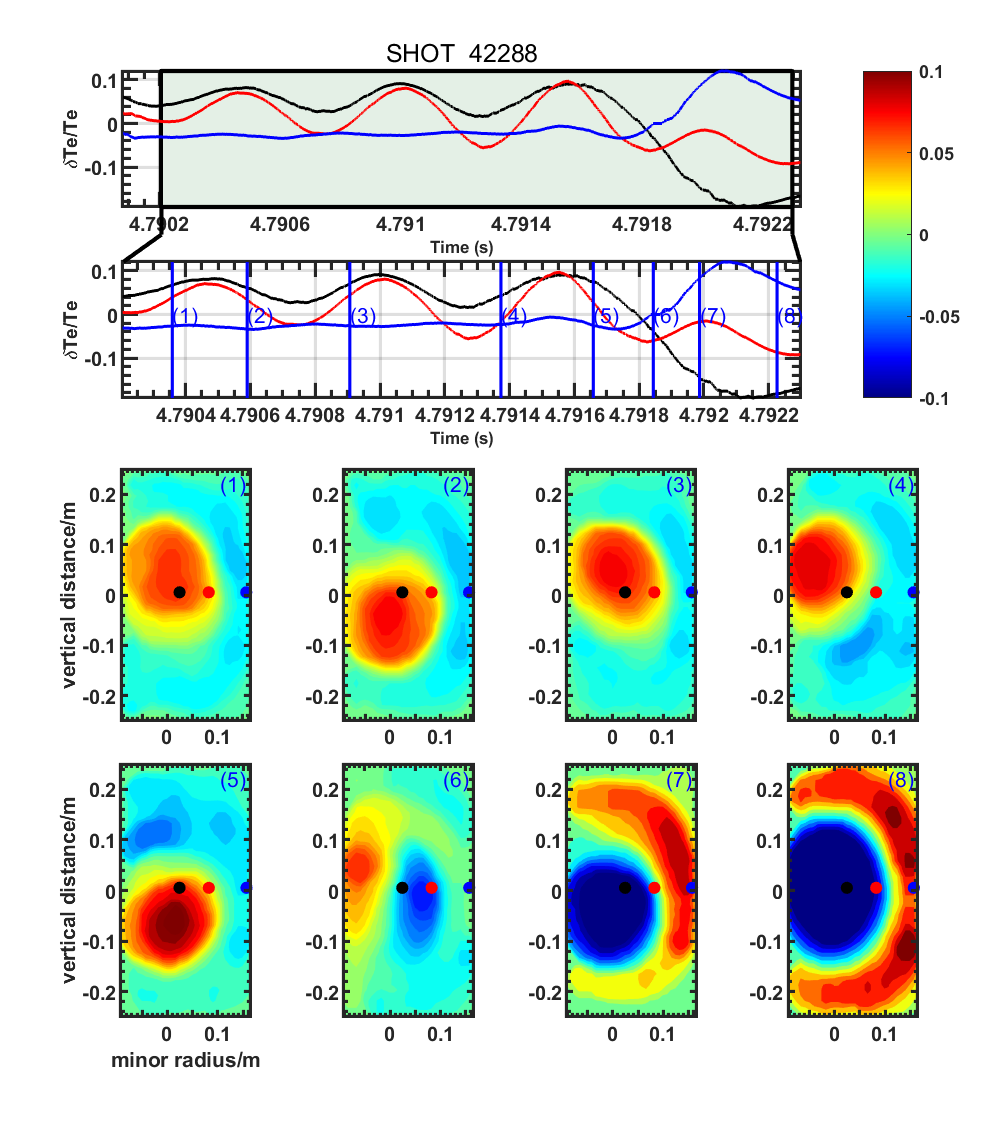
\includegraphics[width=14cm]{image10_1.eps}
  \caption{\label{fig:ECEIimag}EAST 装置中 ECEI 诊断观测到的锯齿破裂演化过程,不同颜色表示温度涨落分布,红色为正、蓝色为负,三条曲线对应矩形窗口中的三个空间位置}
\end{figure}

ECEI 诊断涉及到辐射频率与空间位置的对应关系,辐射强度与温度的对应关系。
\par \noindent
a.空间位置的对应关系
\par 根据经典电动力学知识,托卡马克中电子绕磁力线回旋运动会辐射出电磁波,由于电子回旋运动的非线性效应,电子回旋频率除了基频$f_{ce}$以外还存在该频率的高次谐波成分(\autoref{sec:A1}),因此电子回旋频率可表示为
\begin{equation}
nf_{ce}=n\frac{1}{2π}∙\frac{eB}{\gamma m_e} 
\end{equation}
其中n=1,2,3,…表示谐波次数,γ表示相对论修正因子,B表示托卡马克中纵场强度,B和大半径之间满足反比例关系:
\begin{equation}
B=\frac{B_0R_0}{R}
\end{equation}
这里$B_0$ 、$R_0$表示磁轴处磁场和大半径。由于纵场强度沿大半径方向单调递减(\autoref{fig:charac-f}),沿水平径向观测方向上,回旋频率和纵场强度满足一一对应关系,
\begin{figure}[ht]
  \centering
  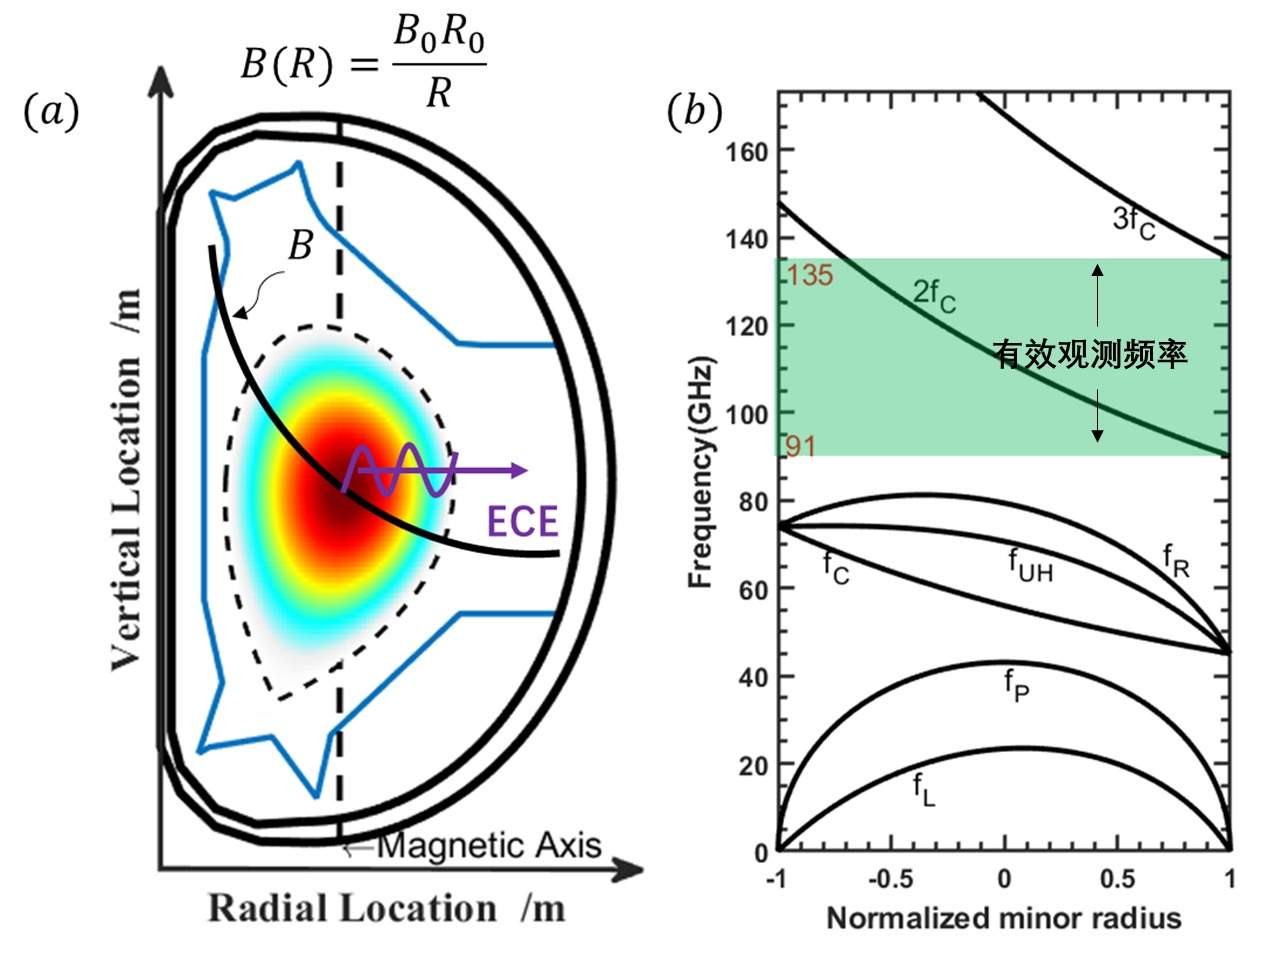
\includegraphics[width=12cm]{image11_2.png}
  \caption{\label{fig:charac-f} (a)托卡马克纵场分布图(b)EAST托卡马克装置下各特征频率分布图,图片为自绘}
\end{figure}
因此可以通过选择不同的频率实现对径向空间位置的分辨。
如\autoref{fig:charac-f}(b)所示,垂直于磁场的特征频率包括电子回旋频率$nf_c$、等离子体频率$f_p$,上杂化频率$f_{UH}$,左旋截止频率$f_{L}$以及右旋截止频率$f_R$等。垂直于磁场传播的电磁波主要存在两种偏振态,其中电场方向平行与磁场的波称为O波,电场方向垂直与磁场的波为X波。X波的截止频率和特征频率中的$f_R$相同,共振吸收频率为$f_{UH}$。O波的截止频率对应特征频率中的$f_p$。为了确保频率和空间位置的一一对应,用于接收的频率必须与其它频率没有重叠,同时该频率能从等离子体中传出来,不被共振或截止。综上所述,只有图中绿色阴影区间的$2f_c$的X波和$f_c$的O波可用于电子回旋辐射诊断,$2f_c$的O波因强度相对X波较弱而被舍弃。
\par 通过光学软件中射线追迹功能可获得ECEI不同极向天线对应的极向观测位置\cite{RN1367,RN1020},因此ECEI具有径向和极向空间分辨能力的二维空间诊断。
\par \noindent
b.辐射强度与温度的对应关系 \par
电子回旋辐射在等离子体区域的输运主要由发射和吸收两个过程决定。在介电常数近似为1的稀薄等离子体中$(ω_{pe}\ll ω$,等离子体频率远小于电磁波频率),辐射输运方程可表示为\cite{RN1414}
\begin{equation}
\frac{\dif  I(\omega)}{\dif s}=\eta(\omega)-\alpha(\omega) I(\omega)
\end{equation}
这里s表示辐射路径,$I(\omega)$表示单位面积单位立体角单位角频率的辐射功率,$\eta(\omega)$表示发射率,$\alpha(\omega)$表示吸收系数,从路径位置$s_1$到$s_2$过程中,该方程的解为:
\begin{equation}\label{eq:optical_s}
I\left(s_{2}\right)=I\left(s_{1}\right) e^{-\tau}+\frac{\eta}{a}\left[1-e^{-\tau}\right]
\end{equation}
其中光学厚度$\tau$的定义是
\begin{equation}
\tau=\int\limits_{s_1}^{s_2}\alpha(\omega)\dif s
\end{equation}
当光学厚度$\tau\gg1$时有
\begin{equation}\label{eq:Is2}
I(s_2)=\frac{\eta}{\alpha}
\end{equation}
此时辐射满足黑体辐射。根据黑体辐射定律,单位路径等离子体发射功率等于其吸收的功率,即$\eta+\alpha B(\omega)=0$,且黑体辐射表面亮度为:
\begin{equation}\label{eq:Itik}
B(\omega)=\frac{\eta}{\alpha}=\frac{\hbar \omega^{3}}{8 \pi^{3} c^{2}} \frac{1}{\exp \left(\frac{\hbar \omega}{T}\right)-1}
\end{equation}
这里考虑的是线极化辐射,所以和课本中黑体辐射公式相差1/2 ,在低频区域$\hbar \omega \ll T$时,我们得到Rayleigh-Jeans公式
\begin{equation}\label{eq:blk}
B(\omega)=\frac{\omega^2T}{8\pi^3c^2}
\end{equation}
结合\autoref{eq:Is2}式和\autoref{eq:blk}式得:
\begin{equation}\label{eq:Te-to-I}
T_e(R(\omega))=\frac{8\pi^3c^2}{\omega^2}I(\omega)
\end{equation}
此时不难看出辐射强度$I(\omega)$与温度$T_e(R)$满足线性关系,原则上通过测量辐射强度结合温度\autoref{eq:Te-to-I}我们就可以准确获得温度。系统对信号强度I的响应通常满足线性关系,即$I_{measure}=k I$,实际上精确测量比例系数k是比较困难的,通常需要借助TS诊断或相关等离子体中的物理过程\cite{RN1381}。目前ECEI信号的主流分析手段是通过测量信号$I_{measure}$的涨落来分析温度的相对涨落,即
\begin{equation}
\frac{\delta T_e}{T_e}=\frac{\delta I_{measure}}{I_{measure}}
\end{equation}
当光学厚度小于1时对应光学薄,对\autoref{eq:optical_s}右侧第二项一阶泰勒展开可得
\begin{equation}\label{eq:optical_s2}
I\left(s_{2}\right)=I\left(s_{1}\right) +\frac{\eta}{a}\tau \approx I\left(s_{1}\right)+ \eta \Delta s
\end{equation}
其中$I(s_1)$表示的是边界反射信号,不考虑反射则为0。此时辐射强度主要取决于发射率$\eta$的形式。如\autoref{fig:etamax}是根据2X波电子回旋辐射方程\eqref{eq:Xradiation}所绘,在固定电子速度条件下电子回旋辐射强度主要由垂直方向电子速度贡献,强烈依赖于
电子垂直方向速度。
\begin{figure}[ht]
  \centering
  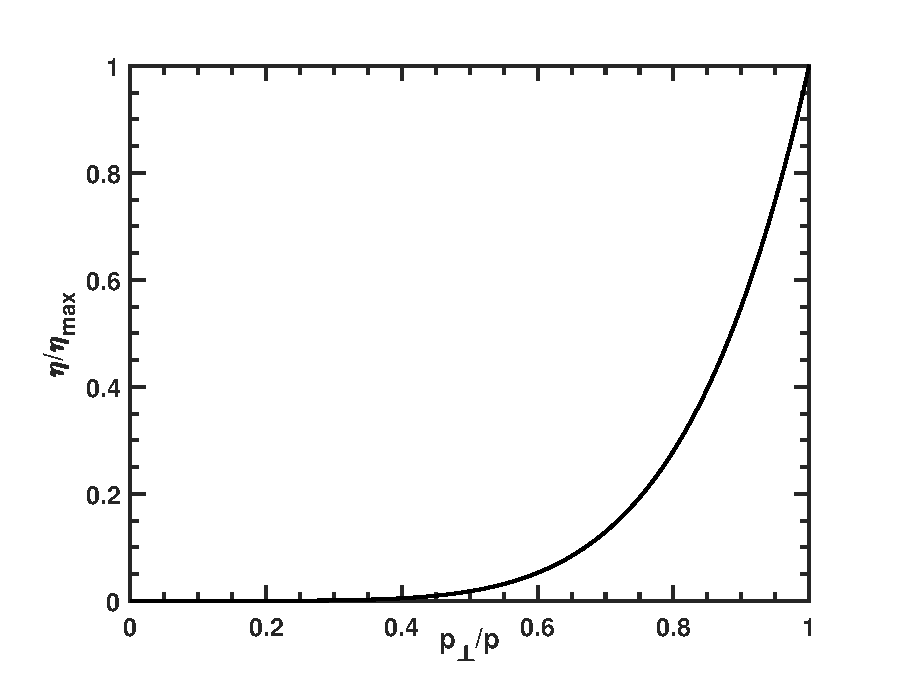
\includegraphics[width=12cm]{etadivideetamax.eps}
  \caption{\label{fig:etamax} 垂直磁场方向传播的2X波辐射强度与电子运动角度之间的关系}
\end{figure}
因此光学薄时电子回旋强度的变化主要反映垂直方向电
子速度的变化。在放电初期或低密度放电过程中,光学厚度一般都小于一,电子
速度分布中非热化分布的电子会产生丰富的辐射现象,通过合适的物理模型解释
辐射现象便是本文研究的主要目的。

%\vspace*{2em}
由于EAST装置大窗口资源有限,ECEI系统处于低杂波系统和NBI系统之间且与NBI系统共D窗口,空间十分狭小。目前中国科大正在致力于合并ECEI和MIR(Microwave Imaging  
Reflectometry)光路。合并光路使科大微波成像诊断系统更加紧凑,适应当下
的空间条件。同时通过ECEI和MIR联合诊断可以实现对托卡马克等离子体同一区域
密度和温度波动同时测
量,对研究边界局域模(ELM)、微撕裂模(MTM)等都具有重要的意义。
MIR利用大口径高斯光学透镜通过收集等离子体截止层处反射的微波信号,实现对
托卡马克截止层密度波动成像\cite{mazzucato2001microwave}。如\autoref{fig:MIR}所示,MIR的微波为系统主动
发射的多频率信号,通过照明光路对微波波前曲率调节实现和等离子体截止层曲率
匹配,这样反射的微波信号才能避免多普勒效应对相位的影响,同时实现最大反
射信号强度,提高成像质量。反射信号经过接收光路投影在天线位置,通过天线
上二极管混频降频后进入中频系统实现对微波信号IQ鉴相,获得相位波动信息。
不同极向位置的天线对应不同极向位置的截止层位置,不同频率的微波信号对应
不同截止层的径向位置,通过这种二维探测阵列实现对密度波动的二维成像。
\begin{figure}[ht]
\centering
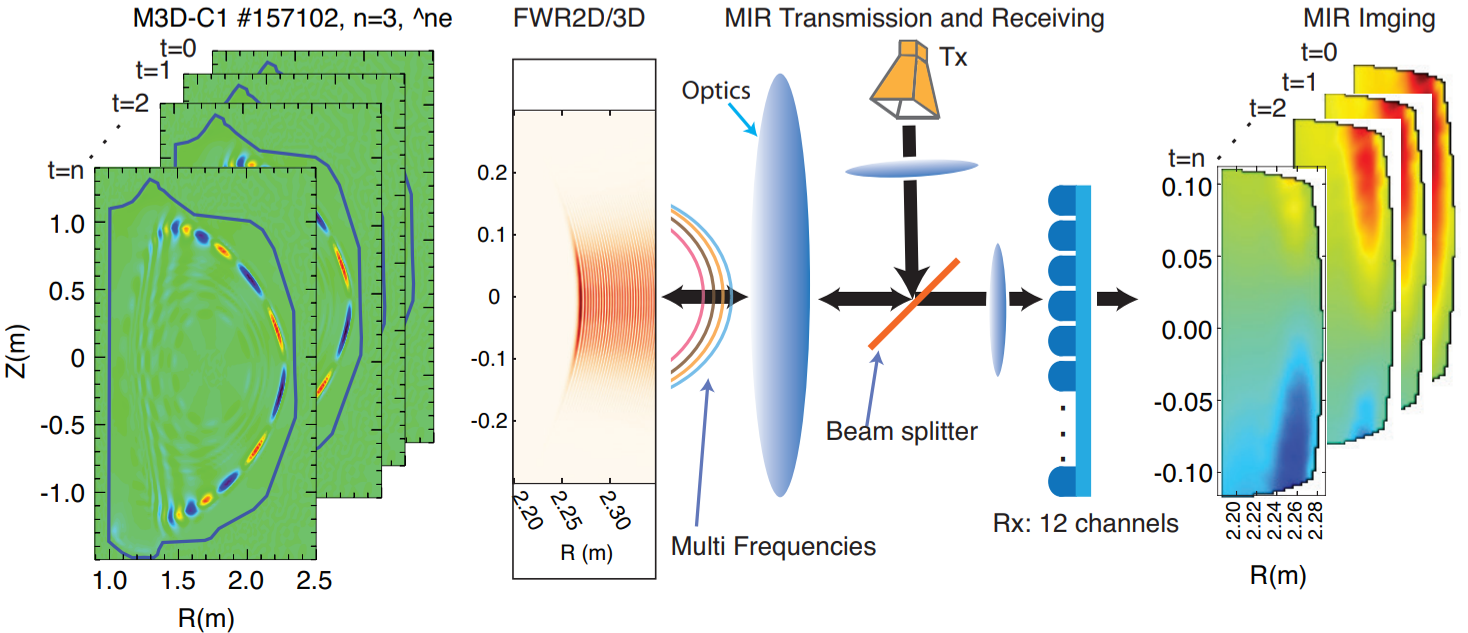
\includegraphics[width=15cm]{image12.png}
\caption{\label{fig:MIR}MIR数值合成诊断图,图片来源自
X.Ren\&M.Chen\cite{RN1190},其中M3D-C1为磁流体程序,用来模拟产生边界
谐频模(EHO),FWR为全波解程序,用来模拟微波在等离子体中的传播。微波
通过照明光路进入等离子体“照亮”截止层,携带截止层相位变化信息的微波经大口径高斯光学透镜投影在接收天线被天线收集,经中频系统检波分析获得最终的密度波动成像图}
\end{figure}
\par 
大口径高斯光学透镜不论在ECEI还是MIR系统中都承担着重要作用,通过多个透镜的组合
可以实现对波前曲率、场曲、聚焦位置、景深等光学参数调节。然而事物的发展
总是具有两面性,透镜组同时会导致微波信号在经过多组透镜时的反射损失增
加。当两套系统合并光路后,原本微弱的辐射的信号还需要进一步一分为二分别
进入两套系统,使得信号弥加珍贵。为了减小信号损失必须要采取相应的手段优
化透镜,降低微波信号在透镜表面的反射损失。其中槽纹表面结构作为广泛应用于可见光学波段增透的技术手段\cite{savin2015black},我们尝试在微波波段同样采用槽纹结构解决透镜表面反射损失问题。
\subsection{大口径高斯光学成像透镜的表面优化}
针对合并光路,减少微波损失的途径主要有三种:1.减小透镜表面反射;2.减小透镜介质损耗正切角对微波的耗散;3.减小分光过程中必要的信号损失。我们选取高密度聚乙烯材料作为光学透镜,高密度聚乙烯材料损耗正切角仅为0.00004-0.001,100Ghz的微波信号单位路径长度损失约为$20\%$,是目前作为微波透镜优质材料。对于第三种方案,由于ECEI和MIR共光路,我们采用罗杰斯分束片将微波信号均分为二分别进入ECEI系统和MIR系统,这样的不足之处是会损失一半有效微波信号。另一种取代罗杰斯分束片的方法是使用频率选择表面(FSS)。由于ECEI和MIR不共频段,原则上可以利用FSS实现选择性分光,使得MIR频率段透射(或反射)进入MIR系统,ECEI信号反射(或透射)进入ECEI系统,实现无损分光。但最后的测试结果并不理想,FSS结构依然有待改进。因此最终可优化的就是第一种:减小透镜表面反射。
\par 透镜表面一般优化方法是贴增透膜,单层增透膜广泛用于可见光波段,通过干涉相消的方法抑制反射波,由于其结构特征只能实现特定频率的波长增透。为了实现宽频增透效果,人们提出了多层膜结构\cite{RN2059}。多层膜结构虽然能实现宽频增透,但是对材料、镀膜精度要求苛刻。对于毫米波透镜,其膜层厚度也需要在毫米量级,在实际操作透镜时难免会因为碰触导致镀膜层破损。大自然里的夜行动物早就进化出了广谱(或者说适应宽波长范围)光学增透结构进而提高夜间视力。20世纪末,人们通过电子显微镜对夜间动物的角膜观测发现在夜间动物的眼角膜上均匀分布高度和距离约200nm的角锥结构\cite{RN693},经研究发现该结构可以有效提高空气和角膜之间,波长在400-700nm之间光的透射率,因此这种表面也称为抗反射结构表面(ARS, Anti-Reflection Structure)。夜间动物的眼睛(如飞蛾)之所以有敏锐的视力,除了视觉感光系统灵敏,大自然在其眼角膜上赋予的角锥结构也使得其具有更加优异的光学利用率,光线可以几乎无损的从空气进入眼角膜内,然后被接收分析处理。目前抗反射结构表面多用于可见光波段,而在微波频段下的应用甚少,微波成像诊断系统主要工作在W波段和F波段,拥有复杂的光学系统,微波在透镜表面的反射会降低信噪比或导致透镜之间的驻波效应。为简化物理模型,我们这里考虑一维槽纹结构作为ARS表面,定量研究它的微波增透效果。\par
如\autoref{fig:1dg}(a)所示,我们以一维槽纹结构为例,把槽纹结构从顶端到底端分割成多个小区间(\autoref{fig:1dg}(b)),在每个区间可以认为是折射率为n的等效介质层(\autoref{fig:1dg}(c)),这样的缓变介质层使得微波能够无反射地从空气传播到介质,因为根据Fresnel反射定律,只有入射层和折射层折射率不一致时才存在反射电场,而在缓变介质层中,由于z处折射率和z+dz(dz→0)处折射率增量dn→0,在任何位置反射率几乎都为零,因此微波能无反射损失从空气进入介质中。以上为ABS表面的增透原理,具体定量分析如下:\par
当电磁波入射在槽纹结构表面时,为了避免高阶衍射对能量的损耗只保留零级衍射,根据光栅方程$2π/λ*(sinθ_i±sinθ_m )=2πm/Λ$,当 m<1时槽纹周期Λ和微波波长$λ$之间需要满足$Λ<λ/(n_s+n_i )$,其中$n_s$表示介质折射率,$n_i$表示入射空间折射率。该不等式能保证电磁波以任何角度入射都只存在零级衍射。根据二阶等效介质理论(EMT, Effective Medium Theory)\cite{RN694},在等效多层矩形堆栈结构中每一层等效折射率大小为:
\begin{figure}[ht]
\centering
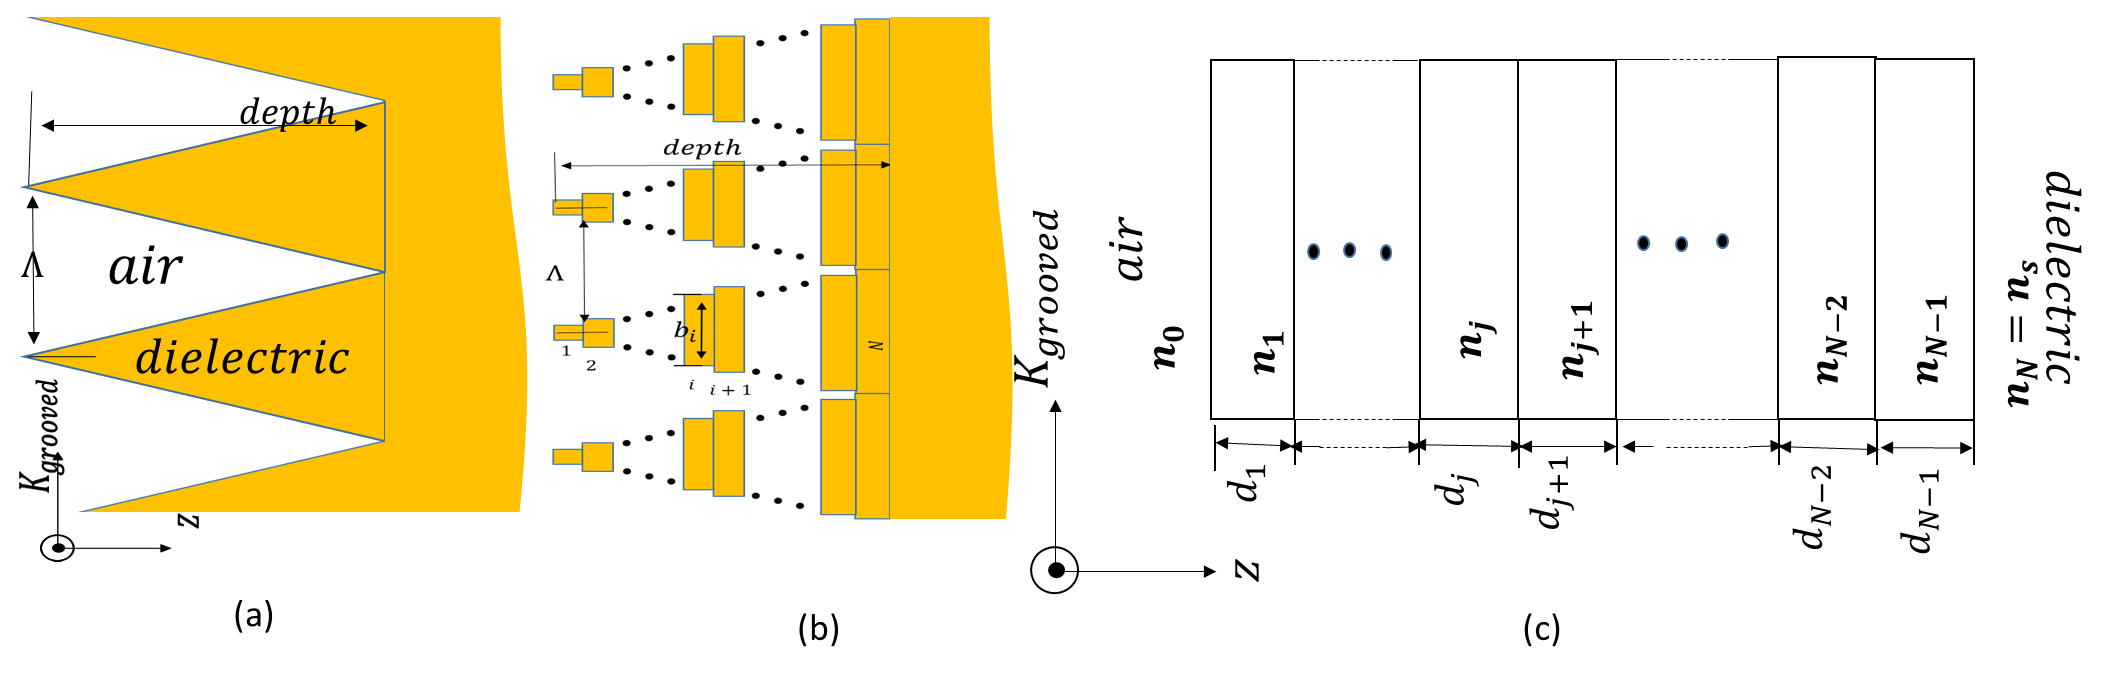
\includegraphics[width=14cm]{image13.png}
\caption{\label{fig:1dg} (a)一维槽纹结构表面,其中黄色部分为介质。(b)将三角结构等效为多层矩形结构堆栈。(c)将多层结构等效为折射率不同的介质堆栈}
\end{figure}
\begin{subequations}
\begin{align}
&\epsilon_{E \perp K}^{(2)}(z)=\epsilon_{E \perp K}^{(0)}(z) {\left[1+\left(\frac{\Lambda}{\lambda}\right)^{2} \frac{\pi^{2} }{3} f(z)^{2}(1-f(z))^{2} \frac{\left(\epsilon_{s}-\epsilon_{i}\right)^{2}}{\epsilon_{0}\epsilon_{E \perp K}^{(0)}(z)}\right] } \\
&\epsilon_{E \perp K}^{(0)}(z)  =f(z) * \epsilon_{s}+(1-f(z)) * \epsilon_{i}
\end{align}
\end{subequations}
$ϵ_s$与$ϵ_i$分别表示介质和入射空间介电系数,$f(z)$为$z$处槽纹结构的占空比。当$z=d$时($d$表示槽纹高度),$f(d)=1$;$z=0$时,$f(0)=0$。$\epsilon_{E\perp K}^2 (d)=\epsilon_s$,$\epsilon_{E\perp K}^2 (0)=ϵ_i$。$E⊥K$表示电场偏振方向和槽纹波矢方向垂直,$E\parallel	K$的情况可参考Daniel H. Raguin \&G. Michael Morris\cite{RN694}。 电磁波电场在j层及j层以内的总反射率为:
\begin{equation}\label{eq:iteration}
\rho_{\mathrm{j}}=\frac{\mathrm{r}_{\mathrm{j}}+\rho_{\mathrm{j}+1} \exp \left(2 \mathrm{i} \delta_{\mathrm{j}+1}\right)}{1+\mathrm{r}_{\mathrm{j}} \rho_{\mathrm{j}+1} \exp \left(2 \mathrm{i} \delta_{\mathrm{j}+1}\right)}
\end{equation}
其中$r_j$表示j和j+1层之间电场的反射率,$δ_j$表示$(2πn_j d_j)/λ  cos⁡(θ_j )$,$n_j$为j层等效折射率,$i=\sqrt{-1}$,$ρ_0$表示槽纹表面总反射率。最终槽纹表面反射率可以通过方程\autoref{eq:iteration}代算出。
\par HDPE材料具有低损耗正切角,可塑性强,被广泛用于微波透镜材料。这里以HDPE材料为例,取$ϵ_s=2.78$,研究不同尺寸的1D三角槽纹对透射率的影响。首先考虑这样一种状态:平面电磁波从空气正入射至无限大介质过程的反射率,其中空气和介质的交界面为无限大平面。利用EMT方法,取三角槽纹表面,槽纹厚度为d,周期为$Λ$,取入射电磁波频率为$87.5GHz$。槽纹结构从顶端到介质等效介电如\autoref{fig:efec}(a)图所示,槽纹结构实现了从空气到介质之间介电常数的缓慢增长。如\autoref{fig:efec}(b)所示,反射率随槽纹厚度d的增加迅速减小,当槽纹厚度达到两倍波长时反射率将减少至不到0.1\% 。ABS表面显著之处在于它不同于增透膜通过干涉的方法实现增透,在理论上这种结构能够实现对满足$λ>Λ(n_s+n_i )$所有频率实现增透,它的最小截止波长为$λ_c=Λ(n_s+n_i )$,这是根据零级衍射条件得到的。
\begin{figure}[ht]
\centering
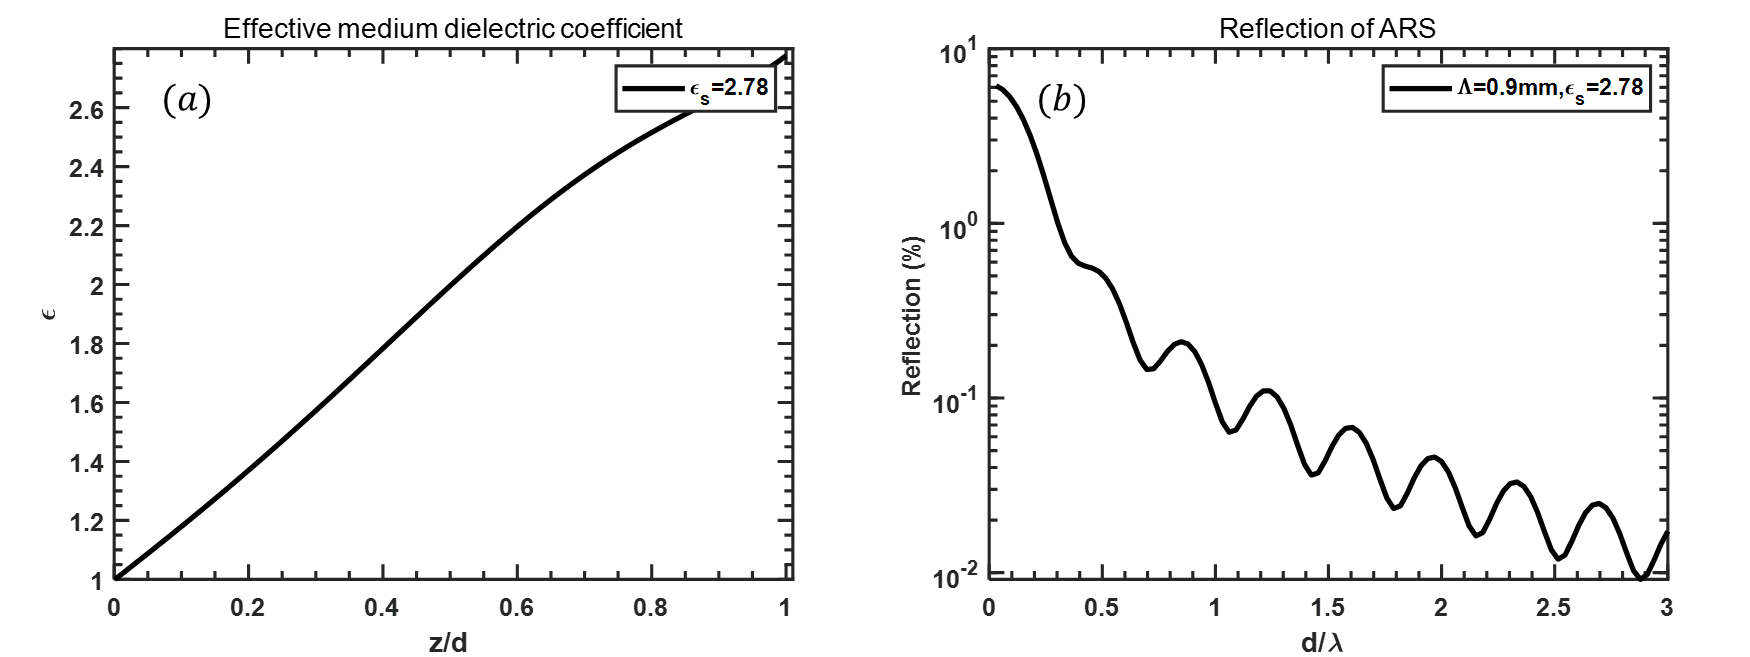
\includegraphics[width=14cm]{image14.png}
\caption{\label{fig:efec}(a)从空气到介质等效介电常数分布。(b)反射率随三角槽纹厚度的变化关系}
\end{figure}
\begin{figure}[ht]
\centering
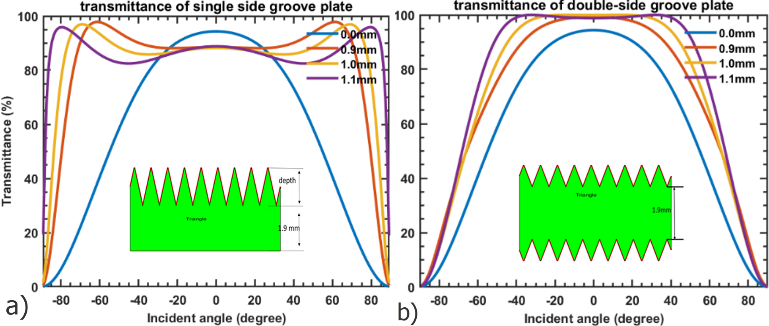
\includegraphics[width=14cm]{image15.png}
\caption{\label{fig:Ta}不同刻槽深度与入射角下单面槽纹板和双面槽纹板透射率,计算中将槽纹结构划分为1000个等效介质层}
\end{figure}
\begin{figure}[ht]
\centering
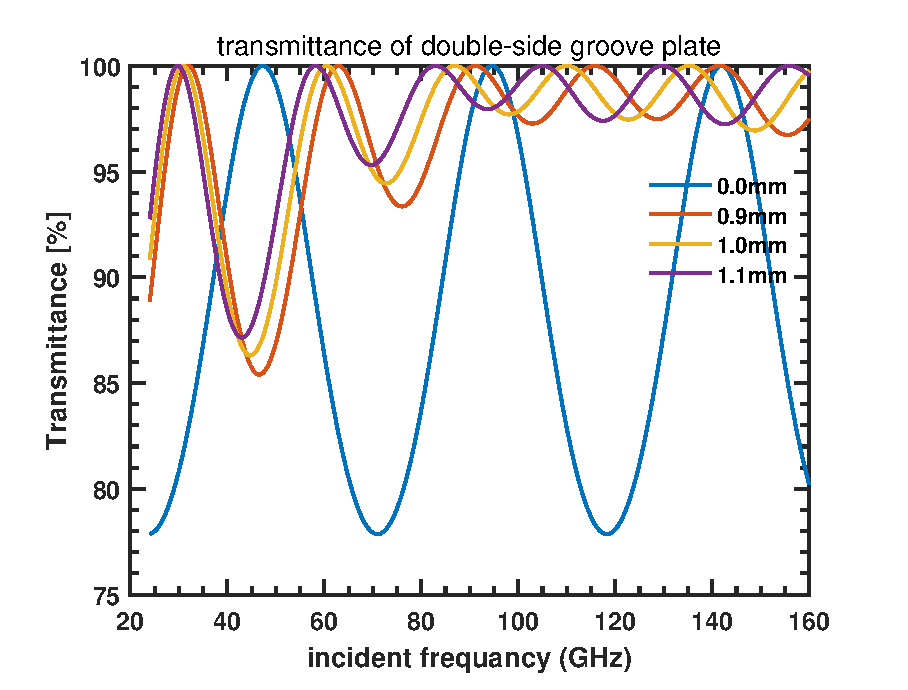
\includegraphics[width=12cm]{Transmittance_Freq.eps}
\caption{\label{fig:Trans_Freq}双面槽纹板不同刻槽深度下垂直入射电磁波透射率与频率变化关系}

\end{figure}
\begin{figure}[ht]
\centering
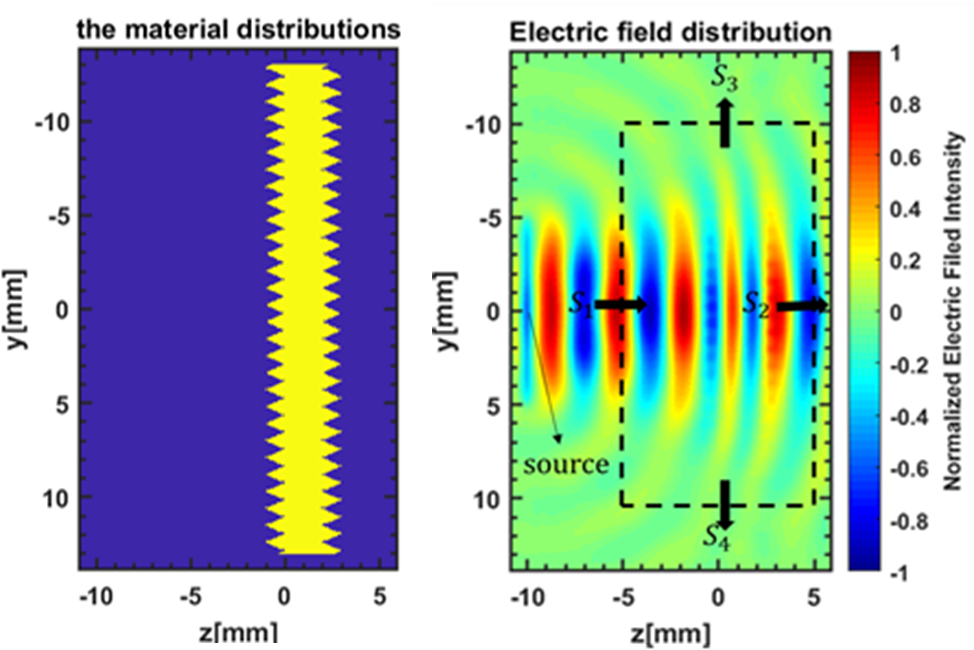
\includegraphics[width=12cm]{image16.png}
\caption{\label{fig:Na}双面一维三角槽纹结构模型以及FDTD计算过程中电场强度分布}
\end{figure}


\par
以上分析只考虑了空气-介质界面反射率的计算,在实际透镜中,我们需要考虑整个电磁波传播经过透镜后的透射率大小,为了方便计算,这里选择透镜形状为平板结构。如\autoref{fig:Ta}所示,平板厚度为1.9mm,频率87.5Ghz,固定槽纹周期$Λ=0.9mm$。如\autoref{fig:Ta}(a)展示了不同刻槽深度下单面槽纹透射率随角度的变化关系。从图中可看出单面槽纹正入射透射率甚至低于无槽纹的平板结构,且单面槽纹透射率随入射角存在两边凸中间凹的趋势,对增透的效果并不理想。反观双面槽纹具有大角度区域的增透效果,且刻槽深度越深,实现增透的角度区间越大。\autoref{fig:Trans_Freq}展示了不同刻槽深度下双面槽纹正入射电磁波透射率和频率的变化关系。对于刻槽深度大于0.9mm的双面槽纹板在频率为60GHZ-160GHZ透区间射率从最低77\%提升到到97\%以上,实现了宽频广角增透效果。我们通过时域有限差分 (Finite Difference Time Domain,FDTD)进一步模拟了双面槽纹电磁波传播过程,并根据能流计算了其对应的透射率。如\autoref{fig:Na}及\autoref{table:Comp},FDTD与EMT得到的结果几乎一致\cite{RN2060}。

\begin{table*}[h]
  \centering
  \caption{\label{table:Comp}FDTD与EMT计算结果对比}
  \label{tab:exampletable}
  \begin{tabular}{lcccccc}
    \toprule
   \multirow{2}{*}{类型}  & \multirow{2}{*}{$S_1$} & \multirow{2}{*}{$S_2$}  &  \multirow{2}{*}{$S_3$}  & \multirow{2}{*}{$S_4$}    &\multicolumn{2}{c}{透射率}
   \\

{}&{}&{}&{}&{}&FDTD&EMT\\

    \midrule
    空气 &342.9&338.3&0.26&-0.29&100\%&100 \\
    平板 & 318.9 &315.8&0.01&-0.01&93.3\%&93.6\%  \\
    单面槽纹 & 303.9 &303.5&0.22&-0.26&89.7\%&89.69   \\
双面槽纹   &338.5&337.4&0.01&0.01&99.72\%&99.17\%\\
    \bottomrule
  \end{tabular}
  \note{注:$S_i$表示第i个面的能流}
\end{table*}

在实验验证过程中,由于HDPE 材料无法通过有效的手段加工出符和要求的槽纹结构,目前只能3D打印制作符合要求的槽纹表面。而打印所用材料ABS (介电常数约2.8\cite{RN2062})其损耗正切角约是HDPE的10倍\cite{RN2061},信号在介质中的损失无法准确评估,透射率测量的实验只能定性分析透射率形状是否和理论一致。如\autoref{fig:exp}(a), 加工的单面槽纹板槽纹周期为0.9mm,高度为1.1mm,板厚约为1.9mm。\autoref{fig:exp}(b)为测量平台示意图,将透镜放在发射源一倍焦距处以构造准平行光,使电磁波入射角方向基本保持一致,最后再通过透镜在一倍焦距处收集透射电磁波。透镜轴线方向相对与测量轴线方向有一定偏角,以避免驻波效应对测量结果的影响,待测平板置于两透镜之间。测量结果如\autoref{fig:expdata}所示,单侧槽纹透射率与模拟结果出现相同的变化趋势,其中右侧有一个点为测量误差导致透射率出现严重偏离。



\begin{figure}[ht]
\centering
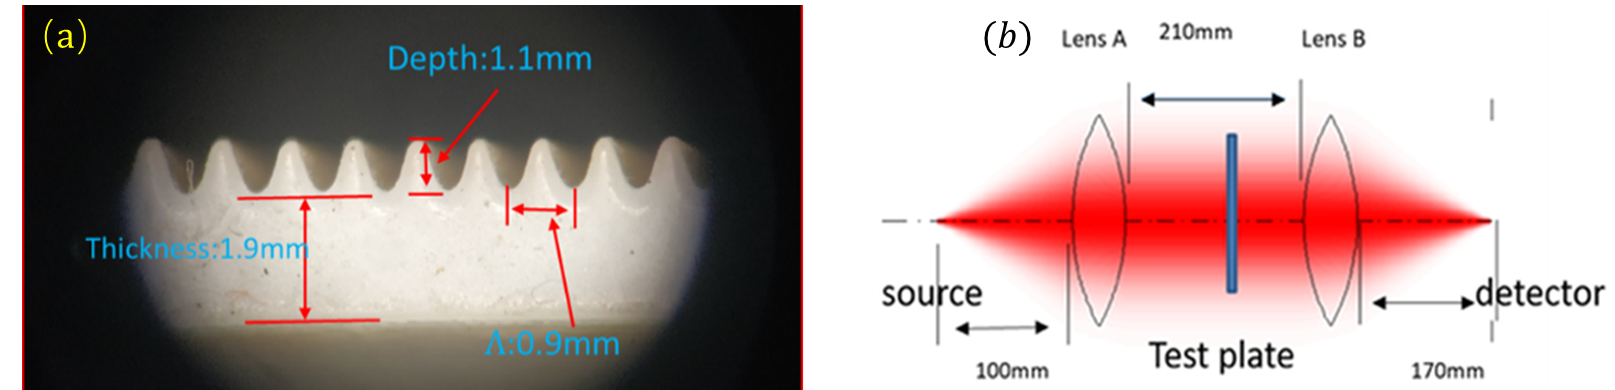
\includegraphics[width=14cm]{image17.png}
\caption{\label{fig:exp}(a)3D打印的单侧槽纹平板(b)透射率测量示意图}
\end{figure}

\begin{figure}[ht]
\centering
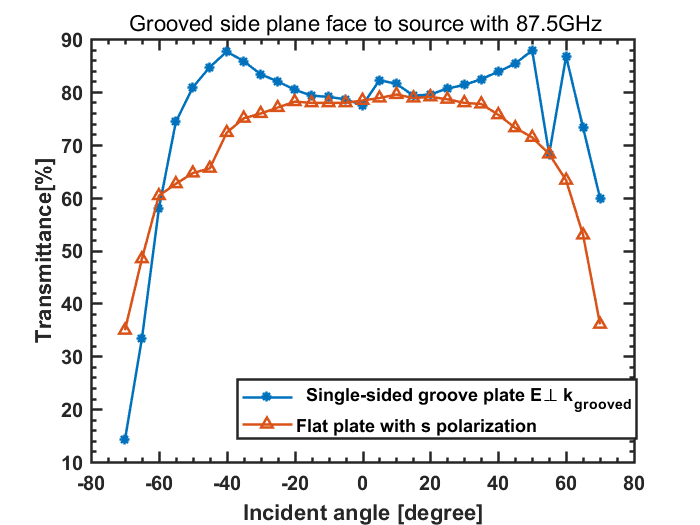
\includegraphics[width=14cm]{image18.png}
\caption{\label{fig:expdata}单侧槽纹板和平板在不同角度下透射率的变化}
\end{figure}

根据理论计算,在 HDPE 材料表面刻蚀周期为 0.9 mm、槽深为 1.1 mm 的一维三角槽纹结构,可将厚度为 1 mm 的平板在 40 GHz–160 GHz 微波正入射条件下的最低透射率由 77 \% 提高至 98 \%以上。该优化设计方案将有助于显著提升电子回旋辐射成像诊断的信噪比,改善成像质量,并为反常电子回旋辐射现象(如反常多普勒效应)的观测提供更加可靠的数据支撑。

%\clearpage
\section{电流爬升期电子回旋辐射}
    本节展示了在 EAST 装置第 64987 次放电(即第 64987 炮)中,ECEI 对反常辐射现象的实验观测结果。 如 \autoref{fig:eceregion} 所示,蓝色矩形区域表示 384 道 ECEI 的观测范围;蓝色虚线为通过 EFIT 反演得到的最后闭合磁面;红色长条则对应 32 道 ECE 的观测位置。 \autoref{fig:eceregion}(b) 中,Vloop 表示放电环电压,Ip 表示等离子体电流,$<n_e>$表示电子弦平均密度,HX 表示硬 X 射线谱强度,SXR 表示软 X 射线强度,ECE 表示电子回旋辐射信号。从 \autoref{fig:eceregion}(b) 可见,放电初期
\begin{figure}[ht]
\centering
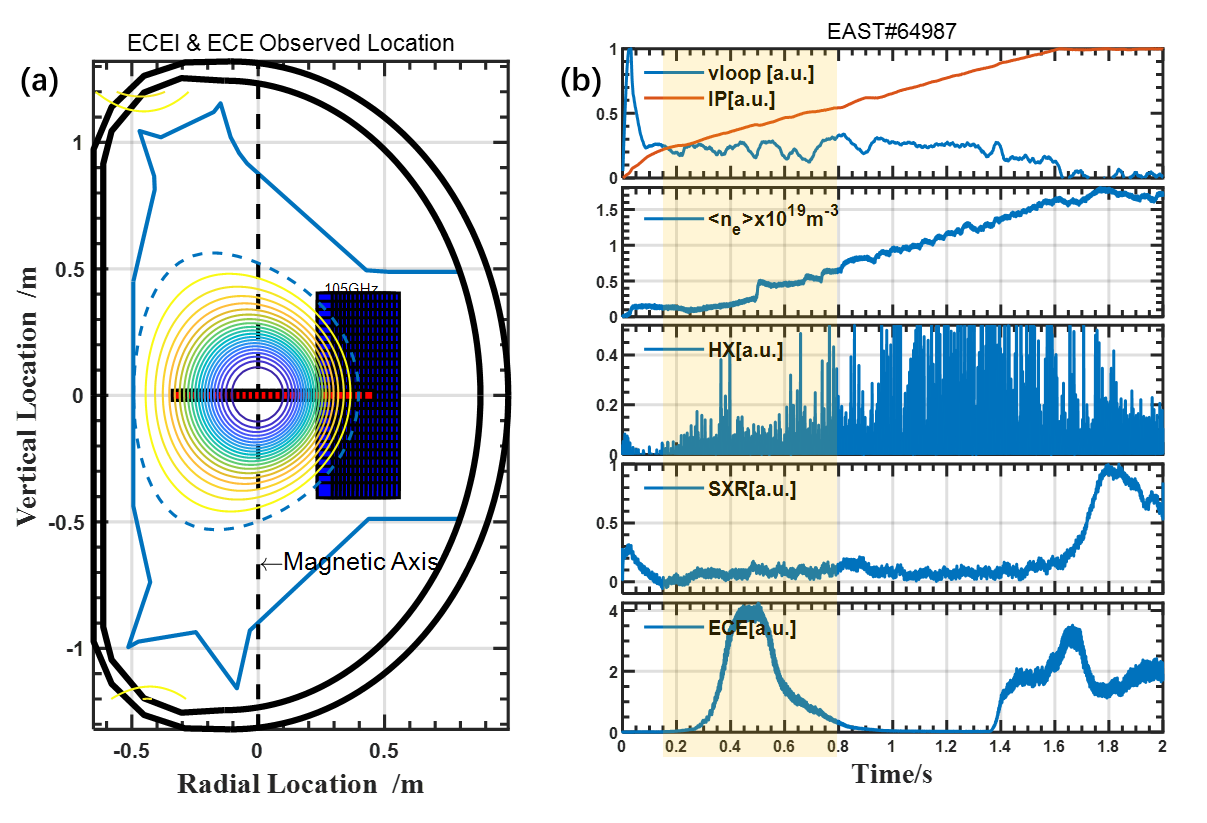
\includegraphics[width=14cm]{image96_2.png}
\caption{\label{fig:eceregion}(a)ECEI观测区域示意图 (b)EAST放电参数图,Vloop表示放电环电压,Ip表示等离子体电流,$<n_e>$表示电子弦平均密度,HX表示硬X射线谱强度,SXR表示软X射线强度,ECE表示电子回旋辐射信号}
\end{figure}
\begin{figure}[ht]
\centering
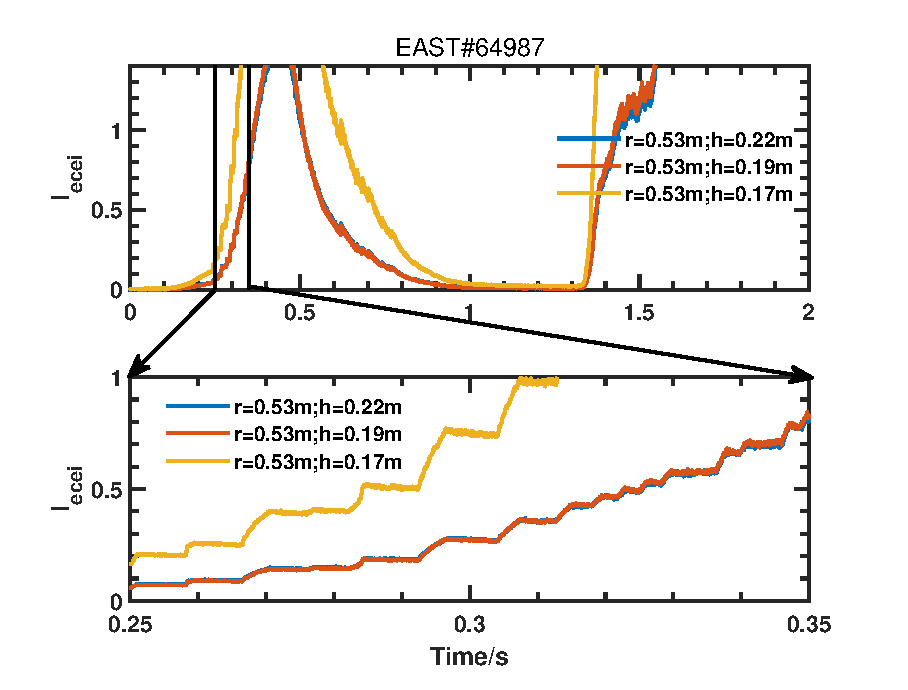
\includegraphics[width=14cm]{image20_1.eps}
\caption{\label{fig:ecestep}电子回旋辐射中的台阶结构,其中$I_{ecei}$表示测量得到的辐射强度,(r,h)表示三道信号所在托卡马克极向剖面空间位置,r表示托卡马克小半径位置,h表示高度}
\end{figure}
环电压Vloop迅速上升紧接着下降,EAST装置 通过消耗欧姆储能产生等离子体,欧姆加热开始驱动等离子体电流爬升,电子密度出现小幅度上升并在之后的0.5s内维持在约$0.2\times10^{19}/m^3$平台。与此同时,从\autoref{fig:eceregion}(b)可看出在0.5s时间SXR和HX无明显变化,说明此时还未产生高能电子,但是电子回旋辐射信号在约0.2s后迅速抬升并在约0.5s达到顶峰,之后缓慢下降,针对该回旋辐射变化的物理机制本文将在\autoref{sec:startup}展开探究。如\autoref{fig:ecestep}所示,为了观察电子回旋辐射信号更多细节特征,我们将ECE信号其中一段时间展开,此时发现了一种显著的现象:在辐射信号抬升的过程中存在一个一个step结构。后来发现,这种类似量子跃迁的现象早在上世纪70年代就已经在实验上发现\cite{RN725}。\par
1976年, D.A.Boyd\cite{RN725}在ATC托卡马克装置上通过测量沿装置大半经方向的电子回旋辐射强度,首次发现了辐射过程出现的step结构。如\autoref{fig:DAB}所示,其中上图表示频率在38GHz-110GHz区间的辐射强度,辐射迅速上升时(上升时间<10μs)伴随着环电压信号的迅速上升,D.A.Boyd将这种现象解释为在出现正电压峰时电子速度空间出现了快速角度散射,导致回旋辐射迅速上升。我认为D.A.Boyd是基于这样一种朴素的物理图像提出了这种猜想:首先系统的环电压与逃逸电子有关,环电压出现正电压峰时说明逃逸电子突然出现阻尼或损失,当逃逸电子出现了快速角度散射时相当于增加了逃逸电子的阻尼。同时被散射的逃逸电子垂直能量增加,因此该过程会导致回旋辐射增加和环电压上升。然而D.A.Boyd对逃逸电子被散射的具体原因并没有给出解释,1979年H. Knoepfel将D.A.Boyd观测到的step现象归因于ADE\cite{RN1030}。时至今日,关于这种现象的讨论已经持续了近50年\cite{RN1863,RN964,RN786,RN1866,RN1554,RN2102,RN1868,RN975,RN1859,RN798},普遍认为产生的原因是ADE。
\begin{figure}[H]
\centering
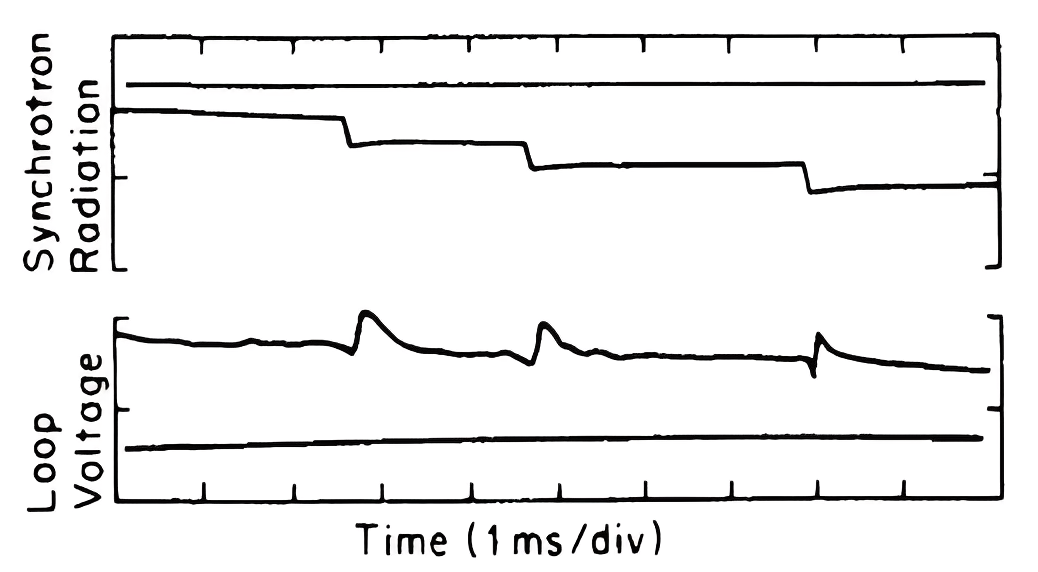
\includegraphics[width=12cm]{image25_1.png}
\caption{\label{fig:DAB}辐射强度‘跃迁’和环电压正电压尖峰出现时间一致,上图轨迹线表示辐射强度,辐射频率以$2ω_{ce}$占主导,下图表示环电压变化(5V/div),水平参考直线表示辐射本底和电压本底}
\end{figure}
\par 因此,可以认为本节所观测到的辐射 step 结构与早期实验中的结果具有较高的一致性,其出现时间与环电压的正电压峰高度相关,说明该现象很可能与等离子体启动阶段逃逸电子的角度散射过程密切相关。结合后续章节中对反常多普勒效应的理论分析与数值模拟,我们将进一步探讨这种辐射增强的物理机制,并尝试从速度空间动力学的角度揭示 step 结构的形成条件及其辐射与逃逸电子分布的关系。





\section{小结}
本章介绍了电子回旋辐射成像诊断的基本原理及其在托卡马克实验中的应用,并提出了光学透镜表面优化方案以提升信噪比。通过对放电初期台前端峰和阶状辐射结构的观测与分析,引出了反常多普勒效应这一关键物理问题,为后续章节开展非热化电子动理学建模与数值模拟研究奠定了理论与实验基础。












% !TeX root = ../main.tex
\chapter{托卡马克非热化电子相关理论及诊断}\label{sec:chapt2}

%\section*{引言}
\vspace{1em}
如果说算法是程序的骨架,那么理论便是程序的灵魂。本章主要介绍动理学计算程序的理论基础。首先介绍均匀磁场背景中非热化电子在静电场下演化的基本物理过程 ,然后通过动理学方程定量描述不同物理过程对电子速度分布函数的影响,最后介绍与非热化电子相关的诊断。

\section{非热化电子相关理论研究}

非热化电子演化涉及到加热\cite{RN1454}、磁重联\cite{RN1917}、以及粒子输运\cite{RN1744}	等过
程,在托卡马克放电中占据着非常重要的地位。非热化电子的研究涉及到速度分布函数的演化 ,不满足
热分布的速度分布函数在碰撞、散射、电磁场扰动、耗散、不均匀背景磁场分布等条件下如何演化是人
们一直关心的问题,动理学方程是描述这类问题的主要手段。通过求解动理学方程可以定量分析电场、
磁场以及电磁波对速度分布的影响,因此动理学模型的选择尤为重要。本节首先定性分析非热化电子在
理想背景中的速度演化行为,然后分别介绍不同物理过程涉及的动理学方程。
\subsection{基本物理过程}
首先我们定性描述非热化电子演化过程中伴随的物理过程。为了参考托卡马克物理条件同时适当简
化物理模型,我们忽略磁场梯度,只局限于分析均匀背景磁场中温度为$T_e$的等离子体在平行磁
场方向电场驱动下的演化。如\autoref{fig:nts}	所示,首先电子会受到库伦碰撞和电场力的相互作
用。 根据卢瑟福散射模型,电子运动碰撞阻力和电子速度的平方成反比,电子运动速度越快,受到的阻
力越小。当电子受到电场的驱动力大于电子的碰撞阻力,电子将会不断受到加速。CONNOR给出了一个
临界电场$E_c=(n_e e^3 lnΛ)/(4πϵ_0^2 c^2 )$\cite{RN1875},当$E>E_c$时,对于速度大于临界速度$v_c^2=(n_e e^3 lnΛ)/(4πϵ_0^2 E)$的电子群,由于碰撞阻尼小于电场驱动力,这部分的电子将会受到
加速从电场中获得能量发展成逃逸电子\cite{RN1744},这种大于临界速度形成的逃逸电子称为初级逃逸
电子。获得足够能量的初级逃逸电子和背景电子有一定几率发生大角度碰撞,当碰撞后的两个电子速度均大
于逃逸临界速度,那么一个逃逸电子就有可能会通过大角度碰撞效应产生两个逃逸电子,然后二变四,四变
八,逃逸电子的数量将呈指数增长,这种现象叫雪崩逃逸\cite{RN1827}\cite{RN1793}。当碰撞后的电子
速度小于逃逸临界速度时,逃逸电子数量便会减少,退化为热电子。随着逃逸电子速度增加到十几兆电
子伏特,同步辐射阻尼机制开始变得重要,直到辐射阻尼和电场力达到平衡,这使得电子的能量存在最
高上限。同时,由于等离子体中存在各种模式的电磁波,当高能电子速度和波满足$ω=\vk∙\vv+nω_{ce}
(n∈Z)$时会通过共振效应将能量传递给波,波被激发后又会反过来和高能电子相互作用通过电磁湍动过
程使高能电子发生角度散射,导致高能电子平行方向动能散射到垂直方向形成超热电子(垂直方向平均能
量$\sim100keV$)。超热电子又会在电场驱动下加速,当速度再次满足共振条件时又会进入到下一个散
射循环,同时超热电子也可能通过回旋辐射以及背景电子碰撞消耗能量,使其辐射能量降低,具有
退化为热电子的趋势。以上几个物理过程需要数值定量分析该过程中速度分布随时间的演化以及对应的电子回旋辐射强度,所用到的物理模型在本节给出。
\begin{figure}
\centering
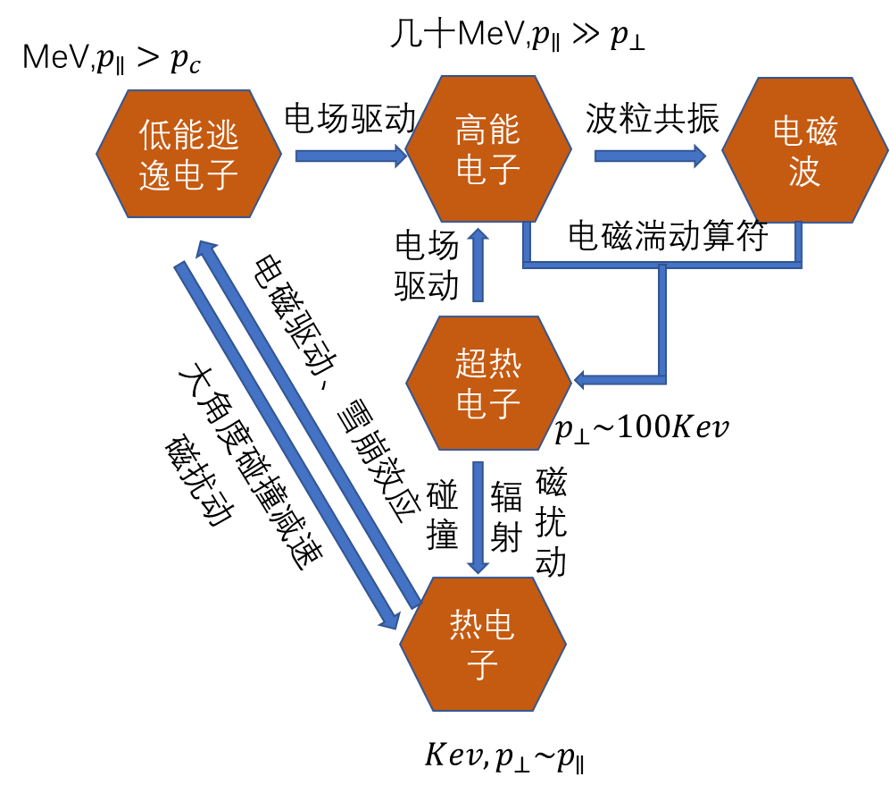
\includegraphics[width=12cm]{image39_1.png}
\caption{\label{fig:nts}非热化电子演化流程图。(注:超热电子的$p_⊥$和$p_∥$具有同等数量级\cite{RN2031},能量可达到百keV,高能电子投掷角几乎为零,但能量为MeV量级,低能逃逸电子表示电子速度和逃逸临界速度同量级,热电子表示具有热平衡分布的电子。)}
\end{figure}
\subsection{动理学分析}\label{sec:kinetic}
定量分析上述过程,必须通过动理学方程描述,其基本方程为\cite{RN1827}:
\begin{equation}
\frac{\partial f}{\partial t}-\mathrm{e} E_{\|}\left(\xi \frac{\partial f}{\partial p}+\frac{1-\xi^{2}}{p} \frac{\partial f}{\partial \xi}\right)+C[f]+\frac{\partial}{\partial \boldsymbol{p}} \cdot \boldsymbol{F}_{\mathrm{rad}} f+D[f]+L[f]=S_{A}[f]+S_{T}[f]
\end{equation}
其中e是电子电荷,$E_∥$是平行磁场的电场强度,$p=m_e γv$,$γ=1/\sqrt{1-(v/c)^2}$,$v$表示速
度,$m_e$表示电子静止质量,$ξ=p_{∥}/p$表示电子运动方向和磁力线夹角的余弦,f表示电子速度分
布函数,且$\int{f\dif^3 p}	=n_e$。$C[f]$表示Fokker-Planck碰撞算符,$F_{rad}$表示同步辐射反作用力,$D[f]$表示准线性扩散算符包括反常多普勒效应、切伦科夫效应以及多普勒效应,$L[f]$表示由于磁扰动引起的逃逸电子损失算符,$𝑆_𝐴[𝑓]$表示由于大角度碰撞导致的雪崩效应,$S_T[f]$表示电子热源项,用来补充损失的逃逸电子。Fokker-Planck碰撞算符$𝐶[𝑓]$和电场驱动项共同描述了热电子在电场驱动下变成初级逃逸电子的物理过程,对应\autoref{fig:nts}中低能逃逸电子和高能电子的形成;同步辐射算符$\frac{\partial}{\partial p}(𝑭_{rad}𝑓)$描述了超热电子以及高能电子辐射减速过程,对应\autoref{fig:nts}中辐射阻尼;准线性扩散项描述了电子和电磁波相互作用导致电子动量方向散射过程,对应\autoref{fig:nts}中电磁湍动散射过程;而雪崩算符$𝑆_A[𝑓]$则描述了超热电子和逃逸电子大角度碰撞过程,对应\autoref{fig:nts}中大角度碰撞减速和雪崩效应。至此所有的物理过程都有了对应的数学模型,下面分别介绍每一项算符:
\
\par 
\noindent
1.Fokker-Planck碰撞算符$C[f]$ \par
 Fokker-Planck碰撞算符描述的是电子通过小角度碰撞散射效应导致速度分布的变化,其方程形
式比具有普适的玻尔兹曼碰撞算符更加简单。Fokker-Planck算符建立过程中一般将粒子分为试探粒子和
主体粒子两部分,将主体粒子近似为热电子背景,试探粒子按照主体粒子的扰动处理,这时Fokker-
Planck项可以用线性算符表示为$C\{f\}=C^l\{f\}=C ̂^{tp}+C ̂^{fp}$,其中试探粒子项$C ̂^{tp} \{f_1,f_M \}$描述的是试
探粒子和主体等离子体碰撞后试探粒子速度分布的扰动,而场粒子项$C ̂^{fp} \{f_M,f_1\}$描述的是受试探
粒子碰撞后主体等离子体速度分布的扰动。当感应电场导致主体分布剧烈改变时才需要考虑非线性算符,该过程理论工作由Braams和Karney在1989年完成\cite{RN2023},并在2017年由Stahl通过计算机完成相应的
过程的数值求解\cite{RN1894}。非线性过程主用在等离子体破裂等研究上,本论文中碰撞算符所采用的方法均为线
性算符。 \par
线性碰撞算符$C ̂^{tp}[f] $可以表示为\cite{RN2025}
\begin{equation}\label{eq:tpfok}
\left.\hat{C}^{t p}=\left(v_{\mathrm{D}}^{\mathrm{ee}}+v_{\mathrm{D}}^{\mathrm{ei}}\right) \mathcal{L}\left\{f_{\mathrm{e}}\right\}+\frac{1}{p^{2}} \frac{\partial}{\partial p}\left[p^{3}\left(v_{\mathrm{S}}^{\mathrm{ee}} f_{\mathrm{e}}+\frac{1}{2} v_{\|}^{\mathrm{ee}} p \frac{\partial f_{\mathrm{e}}}{\partial p}\right)\right]\right]
\end{equation}
其中碰撞频率$\nu_D^{ee}$,$\nu_D^{ei}$ 表征电子-背景电子、电子-背景离子碰撞过程中速度方向散射
速率,$\nu_S^{ee}$描述了电子与背景电子碰撞而减速的速率,$\nu_{∥}^{ee}$表示电子平行方向速度
扩散速率,洛伦兹因子$L=1/2∂/∂ξ(1-ξ^2 )∂/∂ξ$。$\nu_S^{ee}$,$\nu_{∥}^{ee}$,$\nu_D^{ee}$以及$\nu_D^{ei}$分别为
\begin{equation}\label{eq:charnude}
\begin{aligned}
v_{\mathrm{S}}^{\mathrm{ee}} & = \frac{1}{\tau_{\mathrm{c}}} \frac{1}{p} \frac{\ln \Lambda^{\mathrm{ee}}}{\ln \Lambda_{0}} \Psi_{\mathrm{S}}(\bar{p}, \Theta) \\
v_{\|}^{\mathrm{ee}} & = \frac{1}{\tau_{\mathrm{c}}} \frac{2 \gamma \Theta}{\mathrm{p}^{3}} \Psi_{\mathrm{S}}(\bar{p}, \Theta) \\
v_{\mathrm{D}}^{\mathrm{ee}} & = \frac{1}{\tau_{\mathrm{c}}} \frac{2}{p^{2}} \frac{\ln \Lambda^{\mathrm{ee}}}{\ln \Lambda_{0}} \Psi_{\mathrm{D}}(\bar{p}, \Theta), \\
v_{\mathrm{D}}^{\mathrm{ei}} & = \frac{1}{\tau_{\mathrm{c}}} \frac{\gamma}{\mathrm{p}^{3}} \frac{\ln \Lambda^{\mathrm{ei}}}{\ln \Lambda_{0}} Z_{\mathrm{eff}}
\end{aligned}
\end{equation}
其中$\Theta=\frac{T_e}{m_ec^2}$,$Z_{eff}=\sum_j\frac{n_jZ_j^2}{n_e}$表示有效等离子体电荷数,$\tau_{\mathrm{c}}=\frac{4 \pi \varepsilon_{0}^{2} m_{\mathrm{e}}^{2} c^{3}}{n_{\mathrm{e}} e^{4}\ln \Lambda_{0}}$表示相对论碰撞时间,库伦对数分别为:
\begin{subequations}
\begin{align}
\ln \Lambda_{0} & = 14.9-0.5 \ln \left(n_{\mathrm{e}}\left[10^{20} \mathrm{~m}^{-3}\right]\right)+\ln (T[\mathrm{keV}]) \\
\ln \Lambda^{\mathrm{ee}} & = \ln \Lambda_{0}+\frac{1}{k} \ln \left(1+\left[\frac{2(\gamma-1)}{\bar{p}_{\mathrm{Te}}^{2}}\right]^{\frac{k}{2}}\right) \\
\ln \Lambda^{\mathrm{ei}} & = \ln \Lambda_{0}+\frac{1}{k} \ln \left[1+\left(\frac{2 \bar{p}}{\bar{p}_{\mathrm{Te}}}\right)^{k}\right] \\
\bar{p}_{T_{e}} & = \sqrt{\left(\frac{2 T_{e}}{m_{e} c^{2}}\right)}
\end{align}
\end{subequations}
$\ln \Lambda_0$表示热库伦对数\cite{RN1166},$lnΛ^{ee}$和$lnΛ^{ei}$为考虑相对论修正后的库伦对数,其中修正因子k取0.2,用来实现热能和高能之间平滑过渡\cite{RN1818}。$Ψ_D$和$Ψ_S$方程形式分别为:
\begin{subequations}
\begin{align}
&\Psi_{\mathrm{S}}(\bar{p}, \Theta)=\frac{\gamma^{2} \Psi_{1}-\Theta \Psi_{0}+(\Theta \gamma-1) p e^{-\frac{\gamma}{\Theta}}}{p^{2} K_{2}\left(\frac{1}{\Theta}\right)} \\
&\begin{aligned} 
\Psi_{\mathrm{D}}(\bar{p}, \Theta)= & \frac{1}{2 \gamma p^{3} K_{2}\left(\frac{1}{\Theta}\right)}\left(\left(p^{2} \gamma^{2}+\Theta^{2}\right) \Psi_{0}+\Theta\left(2 p^{4}-1\right) \Psi_{1}\right. \\ 
 &\left.+\gamma \Theta\left[1+\Theta\left(2 p^{2}-1\right)\right] p e^{-\frac{\gamma}{\Theta}}\right)
\end{aligned}
\end{align}
\end{subequations}
其中
\begin{align}
\Psi_{0}&=\int_{0}^{\bar{p}} \frac{1}{\sqrt{1+s^{2}}} \exp \left(-\sqrt{1+s^{2}} / \Theta\right) d s \\
\Psi_{1}&=\int_{0}^{\bar{p}} \exp \left(-\sqrt{1+s^{2}} / \Theta\right) d s
\end{align}
$K_2$表示第二类修正贝塞尔函数的二阶形式。
该方程描述的是分布函数在主体背景温度为$T_e$的等离子体中的演化。由于该方程只描述了试探粒子项,没有考虑主体等离子体受到试探粒子碰撞后的变化,因此该方程不满足动量守恒和能量守恒的原则。能量守恒以及动量守恒还需要考虑主体等离子体在受到试探粒子碰撞后自身分布函数的变化$C ̂^{fp}$,这方面的工作由B. Li等人在2011年完成\cite{RN1935},非相对论主体粒子碰撞项可表示为\cite{RN1809}:
\begin{equation}
\hat{C}^{\mathrm{fp}}[f]=\frac{c_{C}}{\pi^{\frac{3}{2}}} \mathrm{e}^{-\bar{v}_{\mathrm{e}}^{-2} x^{2}}\left[\frac{2 x^{2}}{\bar{v}_{\mathrm{e}}^{4}} \frac{\partial^{2} G}{\partial x^{2}}-\frac{2}{\bar{v}_{\mathrm{e}}^{2}} H+4 \pi f\right]
\end{equation}
其中G、H表示Rosenbluth势,满足关系:
\begin{align}
\tilde{\mathrm{v}}_{\mathrm{e}}^{2} \nabla_{\mathrm{v}}^{2} H &=-4 \pi f  \\
 \tilde{\mathrm{v}}_{\mathrm{e}}^{2} \nabla_{\mathrm{v}}^{2} G &=2 H
\end{align}
并且
\begin{equation*}
\begin{aligned}
\widetilde{v}_{e}&=\sqrt{\frac{2 \tilde{T}}{m}}\\
\bar{v}_{e}&=\frac{v_{e}}{\widetilde{v}_{e}}\\
 c_{C}&=\frac{3 \sqrt{\pi}}{4} \bar{v}_{e e}\\
 \bar{v}_{e e}&=\frac{v_{e e}}{\widetilde{v}_{\mathrm{ee}}}\\
\tilde{v}_{\mathrm{ee}}&=16 \sqrt{\pi} e^{4} \tilde{n} \frac{\ln \widetilde{\Lambda}}{3 m^{2} \tilde{v}_{\mathrm{e}}^{3}}\\
 c_{\xi}&=Z_{e f f}+\phi-\Psi+\frac{\bar{v}_{e}^{2} \delta^{4} x^{2}}{2}
\end{aligned}
\end{equation*}
$Z_{eff}$是有效离子电荷数,$x=v/\tilde{v_e}$表示约化速度。$Φ$和$Ψ$分别表示误差函数和钱德拉塞卡函数。实际计算中,由于我们关心的是非热化电子分布在等离子体背景中的演
化行为,而主体等离子体主要涉及电流、电阻、温度等宏观参数,这些参数在模拟中可以根据实验测量
时时更新。因此在处理非热化电子问题时,本论文中Fokker-Planck碰撞算符计算过程只考虑了试探粒子碰撞项,这样虽然失去主体等离子体的演化过程,但研究非热化电子的演化却不受影响\cite{RN1818,RN814,RN1744,RN1800,RN1815}。
\par \noindent
2.辐射阻尼算符$\frac{\partial}{\partial \boldsymbol{p}} \cdot\left(F_{\mathrm{rad}} f\right)$ \par

 在磁化等离子体中,当电子速度增加到相对论速度时,同步辐射逐渐占据主导,导致辐射阻尼直到和电场力平衡,这时候电子平行方向速度将会达到稳定点。电子回旋辐射会导致能量损失,如果垂直方向能量没有补给的话,垂直速度将会不断降低直到为零,但实际上电子和离子的散射会一直提供一部分能量给垂直方向,这样就导致垂直方向速度也存在不为零的稳定点,此时回旋辐射消耗的能量和电子离子散射获得的能量达到平衡。\par
根据A.Stahl2015年发表在PRL上的文章\cite{RN1770},同步辐射扩散项可表示为:
\begin{equation}\label{eq:radforce}
\frac{\partial}{\partial \boldsymbol{p}} \cdot\left(F_{\mathrm{rad}} f\right)=-\frac{1}{p^{2}} \frac{\partial}{\partial p}\left(\frac{\gamma p^{3}\left(1-\xi^{2}\right)}{\tau_{r}} f\right)+\frac{\partial}{\partial \xi}\left(\frac{\xi\left(1-\xi^{2}\right)}{\gamma \tau_{r}} f\right)
\end{equation}
\noindent	其中$\tau_{r}=\frac{6 \pi\left(m_{e} c\right)^{3}}{e^{4} B^{2}}$表示辐射阻尼时间尺度\cite{RN1844},B表示磁场强度。在\autoref{eq:radforce}式右边第一项表示平行方向同步辐射导致的辐射阻尼,第二项表示回旋辐射阻尼项,描述电子回旋辐射导致的角动量损失。\\
3.雪崩算符$S_A [f]$ \par
与Fokker-Planck碰撞算符描述小角度碰撞过程相反的是大角度碰撞过程,该过程的完备描述只能由最具普遍形式的玻尔兹曼碰撞算符给出。初级逃逸电子形成后,它们穿行在主体等离子体背景中时刻面临与背景电子碰撞。当大角度碰撞发生时,逃逸电子有可能会因为碰撞失去能量落入非逃逸速度区间导致逃逸速度减小,或者继续保持在逃逸速度区间,这部分的动理学描述用玻尔兹曼碰撞算符表示为$C_{ee}^B\{f_e,f_{Me}\}$,其中$f_{Me}$是一种热平衡态分布,$f_e=f_{Me}+δf_e$表示等离子体分布,分别由热平衡分布$f_{Me}$和非热平衡分布$δf_e$构成。在计算高能逃逸电子时,$f_{Me}$的速度分布区域远小于$δf_e$,因此在计算过程中将$f_{Me}$简化为$f_{Me}=n_e δ(\vp)$。另一方面,背景电子受到逃逸电子碰撞后获得的速度也有可能产生新的逃逸电子,该过程的玻尔兹曼碰撞算符为$C_{ee}^B \{f_{Me},f_e \}$。
玻尔兹曼碰撞算符利用碰撞微分截面描述了通过两体碰撞导致单位时间分布函数的变化,碰撞算符可以表示为
$C_{a b}\left(f_{a}\right)=\frac{\left(d n_{a}\right)_{c, a b}}{d t d p}$
其中$(𝑑𝑛_𝑎)_{𝑐,ab}$表示a类型的粒子和b类型的粒子碰撞后导致a类型粒子密度的变化。$(𝑑𝑛_𝑎)_{𝑐,ab}$的方程由Lifshitz \& PitaeVski(1981)\cite{RN1938}	和Cercignani \& Kremer(2002)\cite{RN1940} 给出:
\begin{equation}
\left(\mathrm{d} n_{a}\right)_{c, a b}=f_{a}\left(\boldsymbol{p}_{1}\right) f_{b}\left(\boldsymbol{p}_{2}\right) \bar{g}_{\phi} \mathrm{d} \bar{\sigma}_{a b} \mathrm{~d} \boldsymbol{p}_{1} \mathrm{~d} \boldsymbol{p}_{2} \mathrm{~d} t-f_{a}(\boldsymbol{p}) f_{b}\left(\boldsymbol{p}^{\prime}\right) g_{\phi} \mathrm{d} \sigma_{a b} \mathrm{~d} \boldsymbol{p} \mathrm{d} \boldsymbol{p}^{\prime} \mathrm{d} t
\end{equation}
右边第一项是增长项,描述的粒子a因和粒子b碰撞由动量$p_1$散射到p的速率,第二项表示损失项,描述粒子a散射偏离动量p的速率,这里引入了Møller相对速度\cite{RN2058}$g_{\phi}=\sqrt{\left(\boldsymbol{v}-\vv^{\prime}\right)^{2}-\frac{\left(\vv \times \vv^{\prime}\right)^{2}}{c^{2}}}$以及由散射过程中$\vp_1$,$\vp_2\to \vp,\vp'$微分碰撞截面$dσ_{ab}$。将$(dn_a)_{c,ab}$对时间和$\vp$微分并对速度$\vp_1$,$\vp_2$和$\vp'$积分得到碰撞算符为
\begin{equation}
C_{\mathrm{ee}}^{B}\left\{f_{\mathrm{e}}, f_{\mathrm{e}}\right\} \approx C_{\mathrm{ee}}^{B}\left\{f_{\mathrm{e}}, f_{\mathrm{Me}}\right\}+C_{\mathrm{ee}}^{B}\left\{f_{\mathrm{Me}}, f_{\mathrm{e}}\right\} \equiv C_{\text {boltz }}(\boldsymbol{p})
\end{equation}
根据O. Embréus\cite{RN1811}	的计算,雪崩算符用玻尔兹曼碰撞项的勒让德函数形式表示为
\begin{equation}
S_{A}[f]=\Sigma_{L} C_{L}(p) P_{L}(\xi)
\end{equation}
 $P_{L}(\xi) $ 表示 Legendre 函数, $ \mathrm{L}=0, \pm 1 , \pm 2 , \pm 3, \ldots$ , 该模型考虑了高能电子和 背景电子碰撞, 具体表达形式为:
\begin{align}
 &\begin{aligned}
C_{L}\left\{f_{\mathrm{e}}, f_{\mathrm{Me}}\right\} =& \frac{\left(m_{\mathrm{e}} c\right)^{-3}}{2 \tau_{\mathrm{c}} \ln \Lambda} \frac{1}{\gamma p} \int_{p_{0}}^{p^{*}} \mathrm{~d} p_{1} \frac{p_{1}^{3}}{\gamma_{1}} f_{L}\left(p_{1}\right) P_{L}\left(\xi^{*}\right) \Sigma\left(\gamma, \gamma_{1}\right) \\
- &\frac{1}{4 \tau_{\mathrm{c}} \ln \Lambda} \frac{v}{c} f_{L}(p) \int_{\gamma_{\mathrm{m}}}^{\gamma+1-\gamma_{\mathrm{m}}} \mathrm{d} \gamma_{1} \Sigma\left(\gamma_{1}, \gamma\right) 
\end{aligned} \label{eq:CLfefMe} \\ 
 &\begin{aligned}
C_{L}\left\{f_{\mathrm{Me}}, f_{\mathrm{e}}\right\}  =& \frac{\left(m_{\mathrm{e}} c\right)^{-3}}{2 \tau_{\mathrm{c}} \ln \Lambda} \frac{1}{\gamma p} \int_{p^{*}}^{\infty} \mathrm{d} p_{1} \frac{p_{1}^{3}}{\gamma_{1}} f_{L}\left(p_{1}\right) P_{L}\left(\xi^{*}\right) \Sigma\left(\gamma, \gamma_{1}\right) \\
-&\frac{\left(m_{\mathrm{e}} c\right)^{-1}}{4 \tau_{\mathrm{c}} \ln \Lambda} \delta_{L, 0} \frac{\delta(p)}{p^{2}} \int_{p_{0}\left(p_{\mathrm{m}}\right)}^{\infty} \mathrm{d} p^{\prime} \frac{p^{\prime 3}}{\gamma^{\prime}} f_{0}\left(p^{\prime}\right) \int_{\gamma_{\mathrm{m}}}^{\gamma^{\prime}+1-\gamma_{\mathrm{m}}} \mathrm{d} \gamma_{1} \Sigma\left(\gamma_{1}, \gamma^{\prime}\right) \label{eq:CLfMefe}
\end{aligned} 
\end{align}
该方程考虑了粒子的速度分布f,散射角度(这里表示为勒让德级数L)对雪崩效应的贡献,且方程自身满足了密度守恒、动量守恒和能量守恒条件。与Rosenbluth–Putvinski\cite{RN1793} 模型中假设逃逸电子速度无穷大以及Chiu–Harvey\cite{RN1941} 模型中考虑逃逸速度分布但假设逃逸电子速度的投掷角为零相比,这个模型更具完备性。\\
4.磁扰动损失算符$L[f]$\par
由于随机磁扰动造成的逃逸电子损失算符可表示为\cite{RN2076,RN2086}:
\begin{equation}
\begin{aligned}
L[f] & = -\frac{f}{\tau_{\delta B}} \\
\tau_{\delta B} & = \frac{(r-a)^{2}}{4\left|v_{\|}\right| D_{s t}} \gamma^{5} \\
D_{s t} & = \pi R_{\text {eff }}\left(\frac{\delta B_{r}}{B}\right)^{2} \\
R_{e f f} & = R q \pi 
\end{aligned}\label{eq:Harvey}
\end{equation}
其中R表示装置大半经,a表示装置小半径,r表示小半径位置,q表示安全因子,$𝑣_{∥}$表示速度,$𝛾$表示洛伦兹因子。\\
5.电子热源项$S_T[f]$\par
\begin{equation}
{S}_T[f]=\alpha f_m
\end{equation}
其中$α=1-∫4πp^2 F_0 dp$ ,$α$表示添加的热等离子体系数以弥补由于逃逸电子造成的密度损失,$f_M$为归一化热电子分布,$F_0$为分布函数n=0的勒让德系数。\\
6.电磁波散射算符$D[f]$\par
在冷等离子体近似中,磁化等离子体中的色散方程用磁流体模型计算给出。我们可以获通过色散方程获得等离子体中存在的各种本征波,例如阿尔芬波、非寻常波、哨声波、磁声波等、朗缪尔波等。如果考虑非热化电子成分,根据动理学方程中介电常数和分布函数的关系,等离子体可以通过共振的形式激发(或阻尼)本征电磁波,而激发出的电磁波又会反作用于等离子体自身,该过程称为电磁湍动过程\cite{胡希伟2006等离子体理论基础}。\par
为了研究电磁湍动过程,首先需要建立分布函数和电磁波增长率之间的关系,常见的处理方法是将分布函数分成两部分,一部分是冷等离子体部分,该部决定等离子体波的色散关系$\omega=\omega(k,r)$,另一部分为非热化电子分布,这部分的分布函数决定波增长率大小,当增长率远小于频率时,$\omega_r≫\omega_i$,增长率可以通过对等离子体色散关系线性化处理,由一阶扰动展开得到\cite{RN1452}:
\begin{equation}\label{eq:gamma}
\Gamma_{v}=-i \frac{E_{\alpha}^{*} E_{\beta} \omega^{2} \varepsilon_{\alpha \beta}^{A}}{E_{\alpha}^{*} E_{\beta} \frac{\partial}{\partial \omega} \omega^{2} \varepsilon_{\alpha \beta}^{H}}
\end{equation}
增长率包含等离子体会电张量  $\epsilon_{\alpha \beta}$, $\alpha$ 、 $\beta$表示$  \mathrm{x} $、 $\mathrm{y} $、$ \mathrm{z} $ 三个方向电场矢量,  $\epsilon_{\alpha \beta} $ 一般 是复数形式, $ \epsilon_{\alpha \beta}=\epsilon_{\alpha \beta}^{H}+i \epsilon_{\alpha \beta}^{A}$ , 具体推导在 T.H.Six 书 《WAVES in PLASMAS》\cite{RN1836}中给出了详细的过程, 这里只给出其最终结果:
\begin{subequations}\label{eq:disper}
\begin{align}
&\varepsilon_{x x} = \varepsilon+\frac{4 \pi e^{2}}{\omega} \int d^{3} p \sum_{n = -\infty}^{\infty} A_{n} \frac{n^{2} \omega_{c e}^{2}}{k_{\perp}^{2}} J_{n}^{2} \\
&\varepsilon_{x y} = -\varepsilon_{y x} = i g+i \frac{4 \pi e^{2}}{\omega} \int d^{3} p \sum_{n = -\infty}^{\infty} A_{n} \frac{n \omega_{c e} V \sin \theta}{k_{\perp}} J_{n} J_{n}^{\prime} \\
&\epsilon_{y y} = \varepsilon+\frac{4 \pi e^{2}}{\omega} \int d^{3} p \sum_{n = -\infty}^{\infty} A_{n} V^{2} \sin ^{2} \theta J_{n}^{\prime 2} \\
&\varepsilon_{x z} = \varepsilon_{z x} = \frac{4 \pi e^{2}}{\omega} \int d^{3} p \sum_{n = -\infty}^{\infty} B_{n} \frac{n \omega_{c e} V \cos \theta}{k_{\perp}} J_{n}^{2} \\
&\varepsilon_{y z} = -\varepsilon_{z y} = -i \frac{4 \pi e^{2}}{\omega} \int d^{3} p \sum_{n = -\infty}^{\infty} B_{n} V^{2} \sin \theta \cos \theta J_{n} J_{n}^{\prime} \\
&\varepsilon_{z z} = \eta+\frac{4 \pi e^{2}}{\omega} \int d^{3} p \sum_{n = -\infty}^{\infty} B_{n} V^{2} \cos ^{2} \theta J_{n}^{2}
\end{align}
\end{subequations}
\noindent	其中
\begin{equation*}
\begin{aligned}A_{n}= & \frac{1}{\left(\omega-k_{\|} \mathrm{V} \cos \theta-n \omega_{\mathrm{ce}}\right)} \\& \times\left[\frac{1}{V} \frac{\partial f}{\partial p}+\frac{\omega \cos \theta-k_{\|} V}{\omega \mathrm{pV} \sin \theta} \frac{\partial f}{\partial \theta}\right] \\B_{n}= & \frac{1}{\left(\omega-k_{\|} \mathrm{V} \cos \theta-n \omega_{\mathrm{ce}}\right)} \\& \times\left[\frac{1}{V} \frac{\partial f}{\partial p}+\frac{1}{\mathrm{pV} \cos \theta}\left(\frac{n \omega_{\mathrm{ce}}}{\omega \sin \theta}-\sin \theta\right) \frac{\partial f}{\partial \theta}\right]\end{aligned}
\end{equation*}
并且
\begin{equation*}
\begin{aligned}
\varepsilon& \equiv 1-\sum_{e ; i} \frac{\omega_{\mathrm{p}}^{2}}{\omega^{2}-\omega_{\mathrm{c}}^{2}} \\
g &\equiv-\sum_{e ; i} \frac{\omega_{\mathrm{c}}}{\omega} \frac{\omega_{\mathrm{p}}^{2}}{\omega^{2}-\omega_{\mathrm{c}}^{2}}  \\
\eta &\equiv 1-\sum_{e ; i} \frac{\omega_{\mathrm{p}}^{2}}{\omega^{2}} \\\omega_{c e} = \frac{\omega_{c}}{\gamma}, \omega_{c0} &= \frac{-e B}{m_{e}}, \gamma  = \sqrt{1+\left(\frac{p}{m c}\right)^{2}}
\end{aligned}
\end{equation*}
其中被积函数存在奇点,根据Sokhotski-Plemelj理论\cite{RN1837},
\begin{equation}
\frac{1}{\omega-k_{\|} V \cos \theta-n \omega_{\mathrm{cb}}}=P\left(\frac{1}{\omega-k_{\|} V \cos \theta-n \omega_{\mathrm{cb}}}\right)+i \pi \delta\left(\omega-k_{\|} V \cos \theta-n \omega_{\mathrm{cb}}\right)
\end{equation}
P表示积分主值,将\autoref{eq:disper}代入\autoref{eq:gamma},考虑冷等离子体条件得到最终增长率方程为\cite{RN1452}:
\begin{equation}\label{eq:gammab}
\begin{aligned}\Gamma_{\mathrm{b}}= & {4 \pi^{2} e^{2} \int \mathrm{d}^{3} p \sum_{n=-\infty}^{\infty} Q_{n} } \\& \times\left[V \frac{\partial f}{\partial p}+\frac{V}{p} \frac{n \omega_{\mathrm{cb}}-\omega \sin ^{2} \theta}{\omega \cos \theta \sin \theta} \frac{\partial f}{\partial \theta}\right] \\& \left.\times \delta\left(\omega-k_{\|} \mathrm{V} \cos \theta-n \omega_{\mathrm{cb}}\right)\right]\left[\left(E_{x}^{2}-E_{y}^{2}\right) \frac{1}{\omega} \frac{\partial}{\partial \omega} \omega^{2} \varepsilon\right. \\& \left.+2 i E_{y} \frac{1}{\omega} \frac{\partial}{\partial \omega} \omega^{2} g+E_{z}^{2} \frac{1}{\omega} \frac{\partial}{\partial \omega} \omega^{2} \eta\right]^{-1} \\Q_{n} \equiv & \left\{\frac{n \omega_{\mathrm{cb}}}{k_{\perp} V} J_{n} E_{x}+E_{z} \cos \theta J_{n}+i E_{y} \sin \theta J_{n}^{\prime}\right\}^{2}\end{aligned}
\end{equation}
至此,我们获得了电磁波能量演化的微分方程:
\begin{align}
\frac{d \mathcal{E}_{k}(t)}{d t} & = 2 \Gamma_{\mathrm{b}} \mathcal{E}_{k}(t) \\
\mathcal{E}_{k}(t) & = \frac{\epsilon_{0}}{2}\left|E_{k}(t)\right|^{2}
\end{align}
以上介绍了电磁波的产生过程,那么等离子体是如何和电磁波相互作用的呢?这个问题从求解弗拉索夫方程出发:
\begin{equation}\label{eq:vlasov}
\frac{\partial f}{\partial t}+\mathrm{v} \cdot \nabla f+\frac{q}{m} \nabla_{\mathrm{p}} \cdot\left[\left(\mathbf{E}+\frac{\mathbf{v} \times \mathbf{B}}{c}\right) f\right]=0
\end{equation}
其中$∇_p$表示$∂/∂p$.求解该方程中需要用到准线性理论,在准线性理论中有三点假设需要满足:1电磁波的扰动足够小使得线性分析时利用电子未扰动轨道积分依然成立;2电磁波的增长率(衰减率)$ω_i≪ω_r$;3电磁波具有稠密的谱分布使得在等离子体状态演化的时间尺度内任何相干波之间都会因为相混而被破坏。基于这些假设,我们可以将速度分布函数分为$f=f_0+f_1$,其中$f_0$表示零阶量,$f_1$表示一阶量。为了将\autoref{eq:vlasov}表示成准线性形式,我们以电磁波空间和时间周期为积分长度,对\autoref{eq:vlasov}速度空间回旋角和时间积分:
\begin{equation}\label{eq:valsovf0}
\begin{aligned}
\frac{\partial f_{0}}{\partial t} & = -q\left <\int_{0}^{2 \pi} \frac{d \phi}{2 \pi} \nabla_{\mathbf{p}} \cdot\left[\left(\mathbf{E}^{(1)}+\frac{\mathbf{v} \times \mathbf{B}^{(1)}}{c}\right) f^{(1)}\right]\right> \\
\quad & = -\lim _{V \to \infty} q  \int \frac{d^{3} \mathbf{k}}{V} \int_ {0}^{2 \pi} \frac{d \phi}{2 \pi} \nabla_{\mathbf{p}} \cdot\left[\left(\mathbf{E}_{k}+\frac{\mathbf{v} \times \mathbf{B}_{k}}{c}\right) f_{-k}\right]
\end{aligned}
\end{equation}
根据一阶近似条件
\begin{equation}
\left(\frac{d f_{1}}{d t}\right)_{0}=-\mathrm{q}\left(\mathbf{E}_{1}+\frac{\mathrm{v}}{c} \times \mathbf{B}_{1}\right) \cdot \frac{\partial f_{0}}{\partial \mathbf{p}}
\end{equation}
其中下标0表示$f^{(1)}$沿未扰动轨道(r,p,t)空间的变化率,通过积分可得到$f^{(1)}$的方程形式为
\begin{equation}\label{eq:valsovf1}
f_{1}(\mathbf{r}, \mathbf{v}, t)=-\mathrm{q} \int_{-\infty}^{t} d t^{\prime}\left[\mathbf{E}_{1}\left(\mathbf{r}^{\prime}, t^{\prime}\right)+\frac{\mathbf{v}^{\prime}}{c} \times \mathbf{B}_{1}\left(\mathbf{r}^{\prime}, t^{\prime}\right)\right] \cdot \frac{\partial f_{o}\left(\mathbf{p}^{\prime}\right)}{\partial \mathbf{p}^{\prime}}
\end{equation}
对\autoref{eq:valsovf1}空间傅里叶变换后代入\autoref{eq:valsovf0},并将$B_k$表示成$E_k$形式 ,微分算符写为
\begin{equation}
\nabla_{p}=\vec{e}_{\rho} \frac{\partial}{\partial p_{\perp}}+\vec{e}_{\|} \frac{\partial}{\partial p_{\|}}
\end{equation}
这里默认了回旋方向均匀分布,因此忽略了$
\vec{ e}_ϕ  1/p_⊥    ∂/∂ϕ$这一项。通过繁琐的迭代运算,电磁波和等离子体湍动扩散方程最终可表示为\cite{RN1757,RN1815,RN1836,RN1829}
\begin{equation}\label{eq:emwdiffuse}
\frac{\partial f}{\partial t}=\frac{\pi e^{2}}{m_{e 0}^{2} c^{2}} \sum_{n=-\infty}^{\infty} \int d^{3} k \widehat{\Pi} p_{\perp} \delta\left(\omega_{k}-n \Omega-\frac{k_{\|} p_{\|} c}{\gamma}\right) \times\left|\psi_{n, k}\right|^{2} p_{\perp} \widehat{\Pi} f
\end{equation}
其中算符
\begin{equation}
\widehat{\Pi}=\frac{\omega_{k}-\frac{k_{\|} p_{\|} c}{\gamma}}{w_{k} p_{\perp}} \frac{\partial}{\partial p_{\perp}}+\frac{k_{\|} c}{w_{k} \gamma} \frac{\partial}{\partial p_{\|}}
\end{equation}
无量纲动量$p=p_0/mc$,$Ω=ω_{ce}/γ<0$,将 $\hat{Π}$ 转化为$(p,ξ)$坐标得
\begin{equation}
\widehat{\Pi}=\frac{1}{p} \frac{\partial}{\partial p}-\frac{w_{k} \xi-k_{\|} v}{w_{k} p^{2}} \frac{\partial}{\partial \xi}
\end{equation}
其中$p=\sqrt{p_⊥^2+p_∥^2},ξ=p_{∥}/p$ 。能量谱分布$\left|\psi_{n,k}\right|^2$\cite{RN1757} 为:
\begin{equation}\label{eq:Psi}
\left|\Psi_{n, k}\right|^{2}=\left|E_{k x} \frac{n}{z} J_{n}+i E_{k y} J_{n}^{\prime}+\frac{p_{\mid}}{p_{\perp}} E_{k z} J_{n}\right|^{2}
\end{equation}
这里$J_n$表示n阶第一类贝塞尔函数,其中的自变量是$z=(k_⊥ p_⊥ c)/ω_{ce}$ ,利用冷等离子体色散关系得到电场的极化方向为:
\begin{equation}\label{eq:polar}
\begin{pmatrix}
 E_{kx}\\
  E_{ky}\\
E_{kz}
\end{pmatrix}=\begin{pmatrix}
 1\\
 i \frac{\omega_{p e}^{2} \omega_{c e} / \omega_{\mathrm{k}}}{\omega_{\mathrm{k}}^{2}-k^{2} c^{2}-\omega_{c e}^{2}-\omega_{p e}^{2}+k^{2} c^{2} \omega_{c e}^{2} / \omega_{\mathrm{k}}^{2}}\\
\frac{k_{\|} k_{\perp} c^{2}}{\omega_{p e}^{2}+k_{\perp}^{2} c^{2}-\omega_{\mathrm{k}}^{2}}
\end{pmatrix}
\end{equation}
将\autoref{eq:polar}其带入到\autoref{eq:Psi}得:
\begin{equation}
\left|\psi_{n, k}\right|^{2}=\left|E_{k x}\right|^{2}\left|\frac{n J_{n}}{z}+\frac{\frac{J_{n}^{\prime} \omega_{p e}^{2} \omega_{c e}}{\omega_{k}}}{\omega_{k}^{2}-k^{2} c^{2}-\omega_{c e}^{2}-\omega_{p e}^{2}+\frac{k^{2} c^{2} \omega_{c e}^{2}}{\omega_{k}^{2}}}+\frac{p_{\|}}{p_{\perp}} \frac{k_{\|} k_{\perp} c^{2} J_{n}}{\omega_{p e}^{2}+k_{\perp}^{2} c^{2}-\omega_{k}^{2}}\right|^{2}
\end{equation}
关于准线性湍动过程, 我们可以通过微分算符 $ \widehat{\Pi}=\frac{\omega_{k} -\frac{k_{\|} p_{\|}{c }}{\gamma}}{w_{k} p_{\perp}} \frac{\partial}{\partial p_{\perp}}+\frac{k_{\|} c}{w_{k} \gamma} \frac{\partial}{\partial p_{\|}}$ 研究其物 理特征, 在不考虑相对论效应的情况下, 微分算符可以表示为  $\widehat{\Pi}=(1-   \left.\frac{\mathrm{k}_{\|} v_{\|}}{w_{k r}}\right) \frac{1}{p_{\perp}} \frac{\partial}{\partial p_{\perp}}+\frac{k_{\|} v_{\perp}}{w_{k} p_{\perp}} \frac{\partial}{\partial p_{\|}}$ , 其对应的特征线方程满足
\begin{equation}\label{eq:sf}
v_{\perp}^{2}+\left(v_{\|}-\frac{\omega_{k r}}{k_{\|}}\right)^{2}=\xi
\end{equation}
特征线的物理意义是描述物理量扰动的传播方向,数学上是将偏微分方程化为常微分方程\cite{RN2028},这里我们用特征线研究分布函数的演化方向。
\par 关于准线性湍动方程的特征线,Thomas Howard Stix 在著作《WAVES IN PLASMAS》\cite{RN1836}中有一段精彩的描述,书中优美地结合了量子力学和能量守恒定理,对特征线方程所包含的物理给出了精妙绝伦的解释,这里摘录如下:根据相对论理论,物质的能量为$E^2=m_0^2 c^4+p^2 c^2$,我们可以得到$EδE=c^2 p∙δp$,因此有$δE=v∙δp$(其中$c^2 p/E=v,E=γmc^2,p=γmv) $。同时根据量子力学理论,当粒子吸收一个光子能量$ΔE=ℏω_k$后,根据动量守恒,粒子平行方向动量变化为$δp_{∥}=ℏk_{∥}$,平行方向能量变化为$δE_∥=v_∥ δp_∥=v_∥ ℏk_∥$,然后$δE=(δE/(δE_∥ ))δE_∥=(w_k/(k_∥ v_∥ )) v_∥ δp_∥$,原方程$δE=v∙δp$即可表示为
\begin{equation}\label{eq:dsf}
0=v_{\perp} \delta p_{\perp}+\left(1-\frac{\omega_{k}}{k_{\|} v_{\|}}\right) v_{\|} \delta p_{\|}
\end{equation}
在非相对论情况下,对方程\autoref{eq:dsf}积分立刻得到特征线方程\autoref{eq:sf},这也说明了为什么特征线是粒子速度的演化方向。
这个描述很好的解释了方程背后所包含的物理意义,分别从经典电磁学和量子力学得到统一的特征线方程。

等离子体中电子在均匀背景静电场作用下经过一定时间后速度分布等高线如\autoref{fig:difuvec}所示。考虑频率为$\omega$,平行方向波数为$k_z$的波在电子回旋频率为$\omega_{ce}$的等离子体中传播,则特征线的形状是以$(\frac{ω}{k_{z}} ,0)$为圆心的同心圆,分布函数梯度 $-∇_v f$沿着圆的切线方向的投影表示特征线上存在分布梯度的粒子会沿着圆的切线方向扩散,使特征线上速度分布趋于均匀。值得注意的是,由于\autoref{eq:emwdiffuse}中狄拉克函数的存在,只有共振的粒子才会被散射。我们考虑三种共振,取n=-1、0、1,我们得到三种共振速度,分别是反常多普勒共振切伦科夫共振(或朗道共振)以及多普勒共振,对应得共振速度分别是$v_{ade}=(ω+|ω_{ce} |)/k_z $,$v_{landau}=ω/k_z $和$v_{nde}=(ω-|ω_{ce} |)/k_z$ ,只有共振线附近的粒子才能参与共振。这三种共振对应不同的物理现象,我们可以通过这张图直观地描述其物理图像:1.对于多普勒共振(NDE),在密度梯度的驱动下,共振粒子将会沿着该位置圆的右上方切线方向运动,导致粒子平行方向速度和垂直方向速度同时增加,例如应电子回旋共振可利用这种机制实现对等离子体的加热和电流驱动(当然Fisch机制目前认为是是驱动电流的主要机制\cite{RN2131})。2.对于朗道共振(Landau),由于共振位置处在特征线圆的顶点位置,因此该位置的密度梯度将会驱动粒子平行方向运动,以抹平共振速度附近电子速度分布的不均匀性。3.对于反常多普勒共振(ADE),在梯度驱动下,粒子将会沿着特征线切线的左上方运动,这意味粒子在反常多普勒共振下平行方向速度减小而垂直方向速度将会增加。这里我们做一个大胆的猜想,反常多普勒共振线会导致粒子平行方向速度减速,垂直方向增大,那么这样的共振线像不像一座堤坝?粒子加速至共振速度被减速‘反弹’,同时垂直方向速度增大。粒子减速脱离共振后,又会在静电场作用下加速,又一次和共振速度相遇,然后又重复上述过程。这样周而复始,粒子是不是就像是遇到了堤坝,平行方向速度出现了阈值,垂直方向速度‘水位’不断升高?这种现象在第四章粒子模拟中得到了验证。
\begin{figure}
\centering
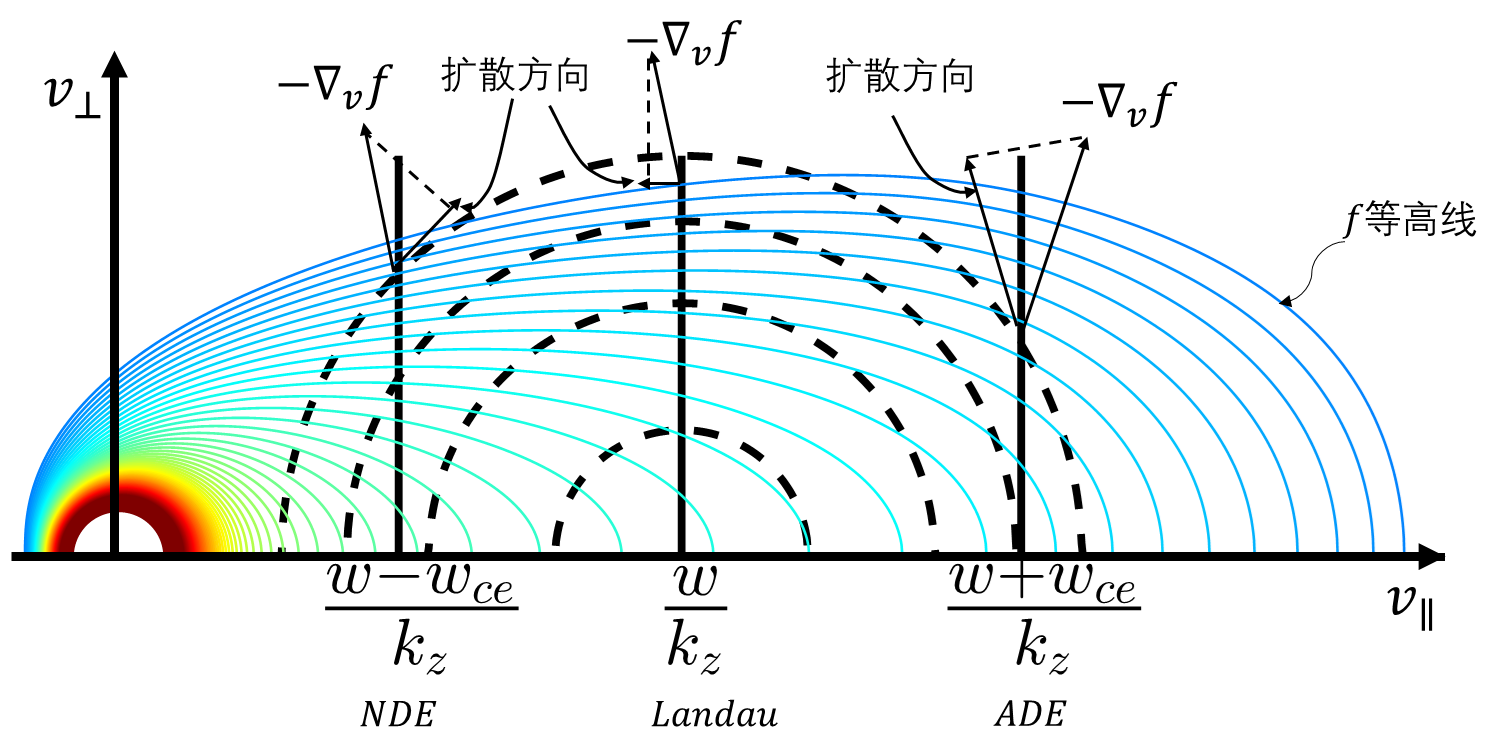
\includegraphics[width=14cm]{image40_1.png}
\caption{\label{fig:difuvec}特征线及多普勒共振、朗道共振与反常多普勒共振对应的电子速度扩散方向,其中虚线表示不同共振能量所在的特征线,只有与共振速度相交的位置才会出现动量散射}
\end{figure}\par

\section{非热化电子诊断方法 }

托卡马克中电子在磁场中运动会受到磁场的洛伦兹力,和周围电子离子的库伦力,以及感应电场对电子的静电力,绕大环方向运动的向心力等。这些力作用在电子上使电子具有丰富的运动状态,导致电子具有轫致辐射、电子回旋辐射、同步辐射等特征,不同能量的电子偏向不同的辐射类型。
\begin{figure}[ht]
\centering
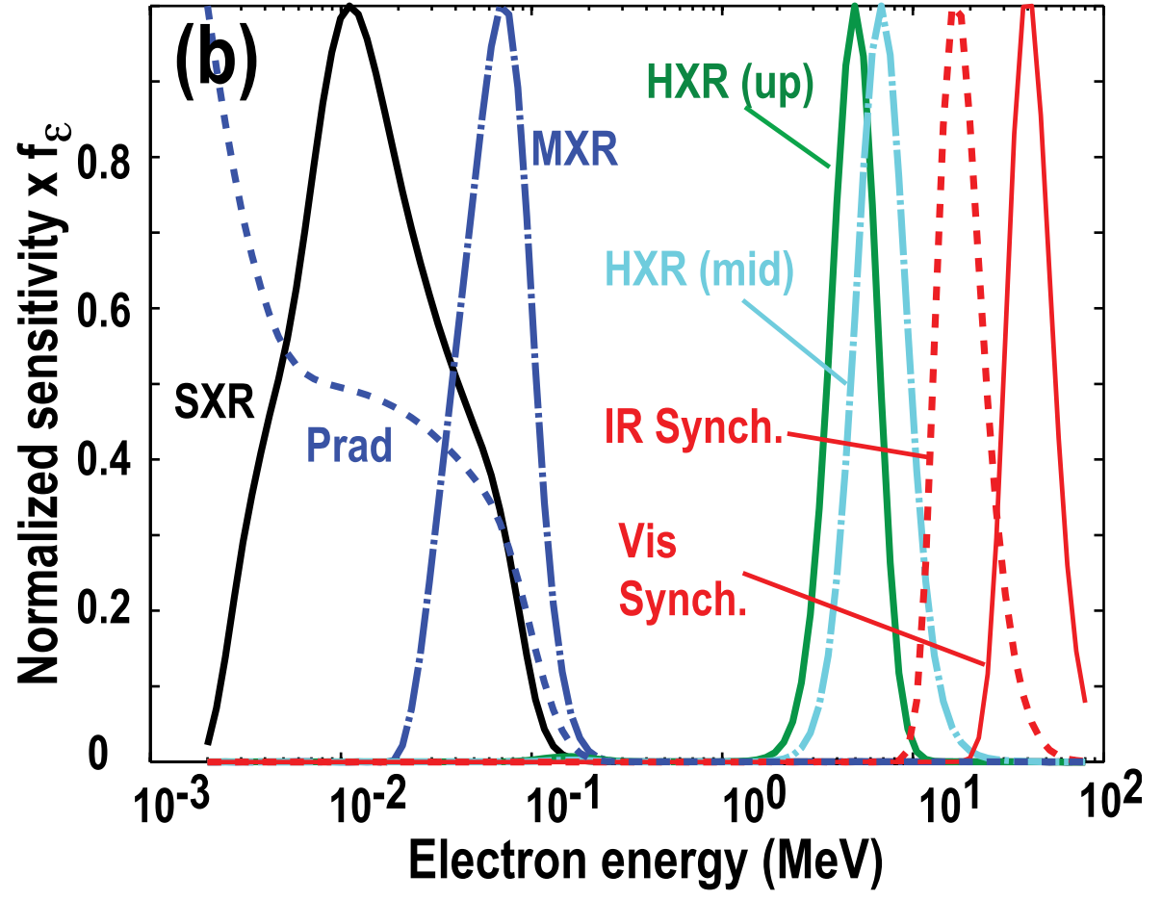
\includegraphics[width=12cm]{image41.png}
\caption{\label{fig:spec}不同辐射诊断对应的电子能量探测区间,图片来自\cite{RN1435}}
\end{figure}\par
尽管托卡马克中电子能量会由于辐射和约束能力而存在上限,非热化电子能量覆盖范围却可以从经典放电中热电子的几keV到逃逸电子中十几MeV,如此宽的能量覆盖范围导致一种诊断不能把非热化电子的速度分布特征诊断清楚。由于非热化电子的辐射谱强度分布和其携带能量有关,具有动能MeV电子的轫致辐射谱主要处在软X射线和硬X射线波段\cite{RN972},毫米波波段可以用来诊断垂直磁场方向能量keV到百keV的非热化电子\cite{RN1356},而几十MeV的高能逃逸电子在环向弯曲磁场中的加速运动产生的同步辐射主要处在红外波段以及可见光波段\cite{RN973,RN956}。因此不同能量的电子具有不同的辐射特征,相应的诊断方法也不相同。如\autoref{fig:spec}所示,其中SXR表示软X射线辐射诊断,用来诊断能量在2-10~keV的电子,Prad表示热辐射诊断用来诊断能量在100~keV以下能量的电子,MXR表示Mid X-ray辐射诊断,用来诊断能量在20-100~keV区间的电子,HXR表示硬x射线诊断,用来分析能量在1-10~MeV区间的逃逸电子,IR远红外段诊断用于分析动能在10-50~MeV的逃逸电子,而Vis Synch表示可见光波段诊断,用于诊断能量区间在30~MeV以上的逃逸电子\cite{RN1435}。
\subsection{轫致辐射诊断}
轫致辐射是托卡马克中最广泛用于诊断逃逸电子或非热化电子的诊断工具之一。轫致辐射是带电粒子与原子或原子核发生碰撞导致速度急剧改变发出的辐射。当逃逸电子被等离子体离子散射时,它的轫致辐射可以认为是“薄靶”的体轫致辐射,通过观测这些辐射可以获得逃逸电子能量信息;当逃逸电子轰击等离子体偏滤器/限制器时,它的轫致辐射相当于是“厚靶”的表面轫致辐射\cite{RN1744}。轫致辐射谱具有连续分布的特征,根据频率一般分为软X射线波段和硬X射线波段。
在软 X射线能段(光子能量1-30keV),通常采用半导体探测器,如EAST上软X射线能谱诊断[128](Soft X-ray pulse height analyzer, SXPHA)采用的是硅漂移探测器(Silicon Drift Detector,SSD)。其原理是入射X光被SSD吸收并激发电子空穴对,在探测器的偏压电场作用下形成原始电流,原始电流信号经过放大器后形成振幅正比于入射X射线能量的脉冲电压信号,脉冲电压信号进入多道分析仪(Multi-Channel Analyzer,MCA)处理成数字信号获得X射线能谱分布。如\autoref{fig:Xray}(b)为EAST放电过程中由SXPHA测得的能谱分布,由于光子能量在1-30keV区间的软X射线辐射基本都是低能量电子辐射谱(部分由杂质中性原子激发退激发过程产生的线辐射频率也在这个区间,如Ar的Ka谱,Ti的Ka谱等),低能量的电子速度分布通常假设具有热分布特征,因此通过能谱图可以拟合出电子的热温度,如\autoref{fig:Xray}(c)(d)所示。
\begin{figure}[ht]
\centering
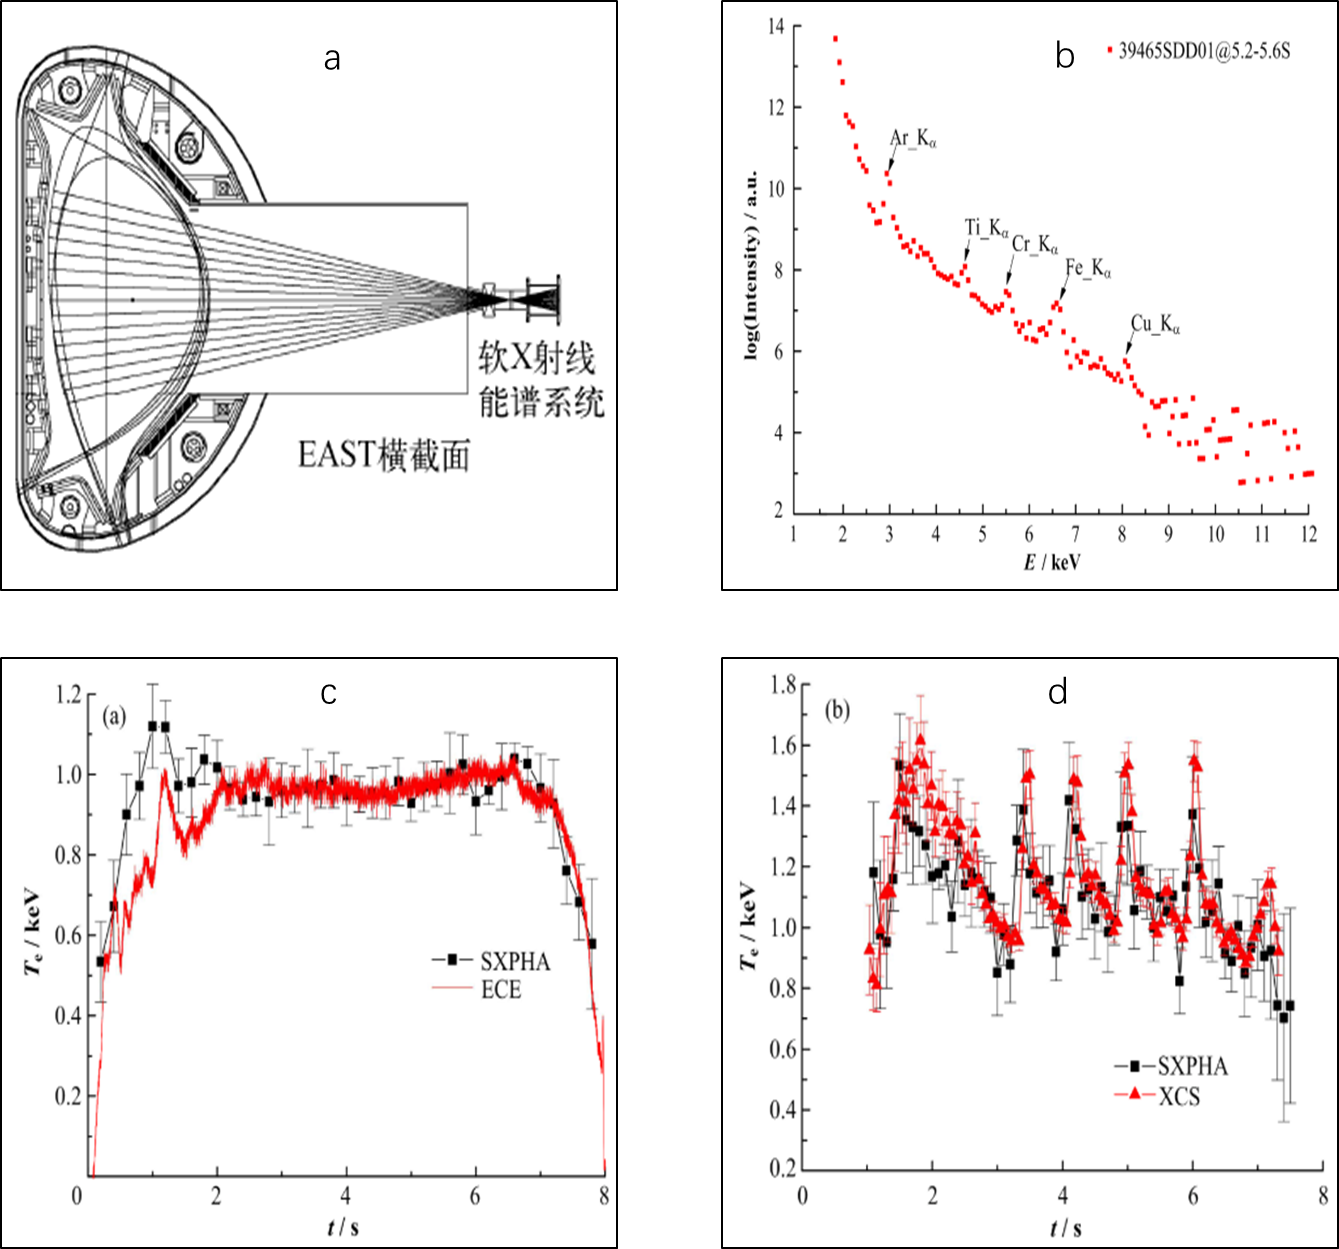
\includegraphics[width=12cm]{image42.png}
\caption{\label{fig:Xray}(a)EAST装置上SXPHA诊断空间布局(b)\#39465炮在5.2-5.6时刻软X射线能谱(c)SXPHA获得电子温度与ECE 辐射温度对比(d)SXPHA所测电子温度与弯晶谱仪所测电子温度对比(图片来自\cite{RN1491})}
\end{figure}\par
  硬X射线诊断中,垂直快电子轫致辐射诊断\cite{RN6}(Fast electron bremsstrahlung diagnostic,FEB)主要用来分析电子垂直方向能量处在30-300keV区间的电子。2018年,华中科技大学J-TEXT托卡马克装置上利用垂直FEB诊断实现了对放电初期间逃逸电子不稳定性的观测\cite{RN6}。该诊断采用CdZnTe 探测器,相对于传统Si和高纯锗等传统半导体探测器,CdZnTe作为一种新型半导体探测器具有体积小,室温可用,分辨率高等优良品质。通过合适的光路设置,如\autoref{fig:JTEXT},FEB可以实现对非热化电子空间分布的探测。除此之外,用于硬X射线能谱诊断还有碘化钠(NaI)闪烁体阵列\cite{RN956}、碲化镉(CdTe)探测器阵列\cite{RN957}	等,这里不再一一赘述。  
\begin{figure}[ht]
\centering
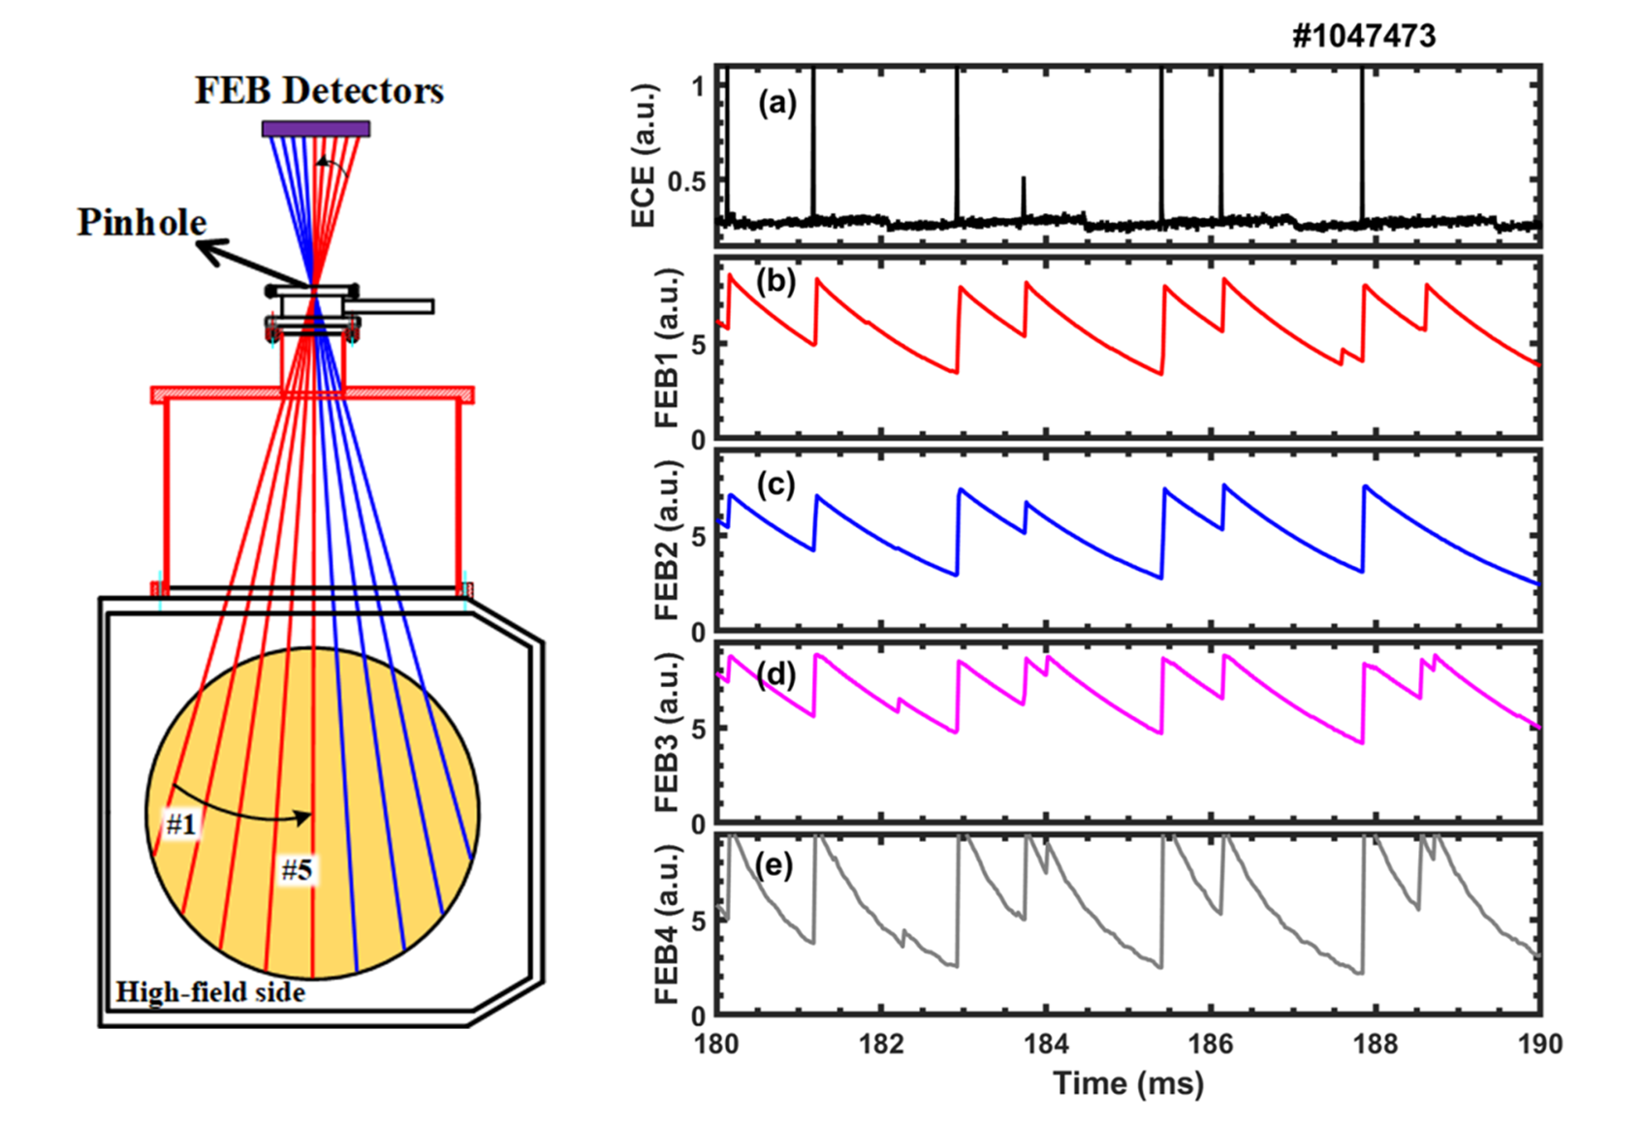
\includegraphics[width=12cm]{image43.png}
\caption{\label{fig:JTEXT}左图为J-TEXT上FEB诊断光学设置,右图表示J-TEXT放电中观测到的ECE辐射信号和FEB信号\cite{RN6}}
\end{figure}
%\clearpage
\subsection{同步辐射诊断}
 在托卡马克领域,“同步辐射”通常指的是磁场中相对论性电子的光辐射,主要取决于电子的动能和螺旋角\cite{RN990},而“回旋辐射”指的是磁场中的非相对论性电子的光辐射,主要取决于电子垂直方向的动能。如\autoref{fig:synchrotron1},同步辐射具有高能量、定向性特征,辐射角锥主要沿着电子运动方向,探测器接收光路只有沿着电子运动方向才能观测到。因此探测相机接收光路一般都在中平面沿着托卡马克环向方向,例如EAST 可见光相机(\autoref{fig:synchrotron2}(a))\cite{RN1885}和TEXTOR远红外光相机(\autoref{fig:synchrotron2}(b))\cite{RN1878}	等。
\begin{figure}[ht]
\centering
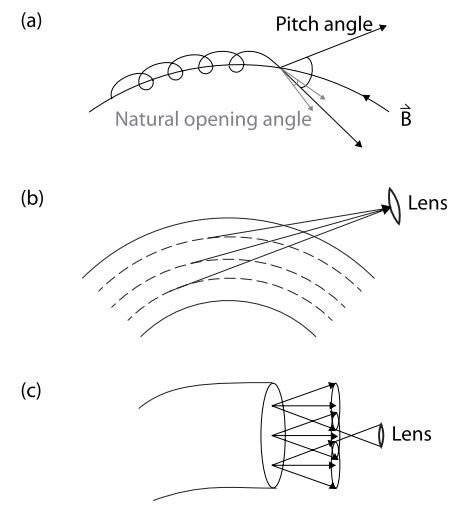
\includegraphics[width=12cm]{image44.png}
\caption{\label{fig:synchrotron1}(a)逃逸电子的同步辐射运动的俯仰角和同步辐射的辐射开口角度(b)托卡马克环向切面,不同磁面逃逸电子辐射方向(c)极向切面:来自不同区域的逃逸电子发出的同步辐射。只有在发射锥内的同步辐射被透镜收集。图片来自\cite{RN1878}}
\end{figure}

\begin{figure}[ht]
\centering
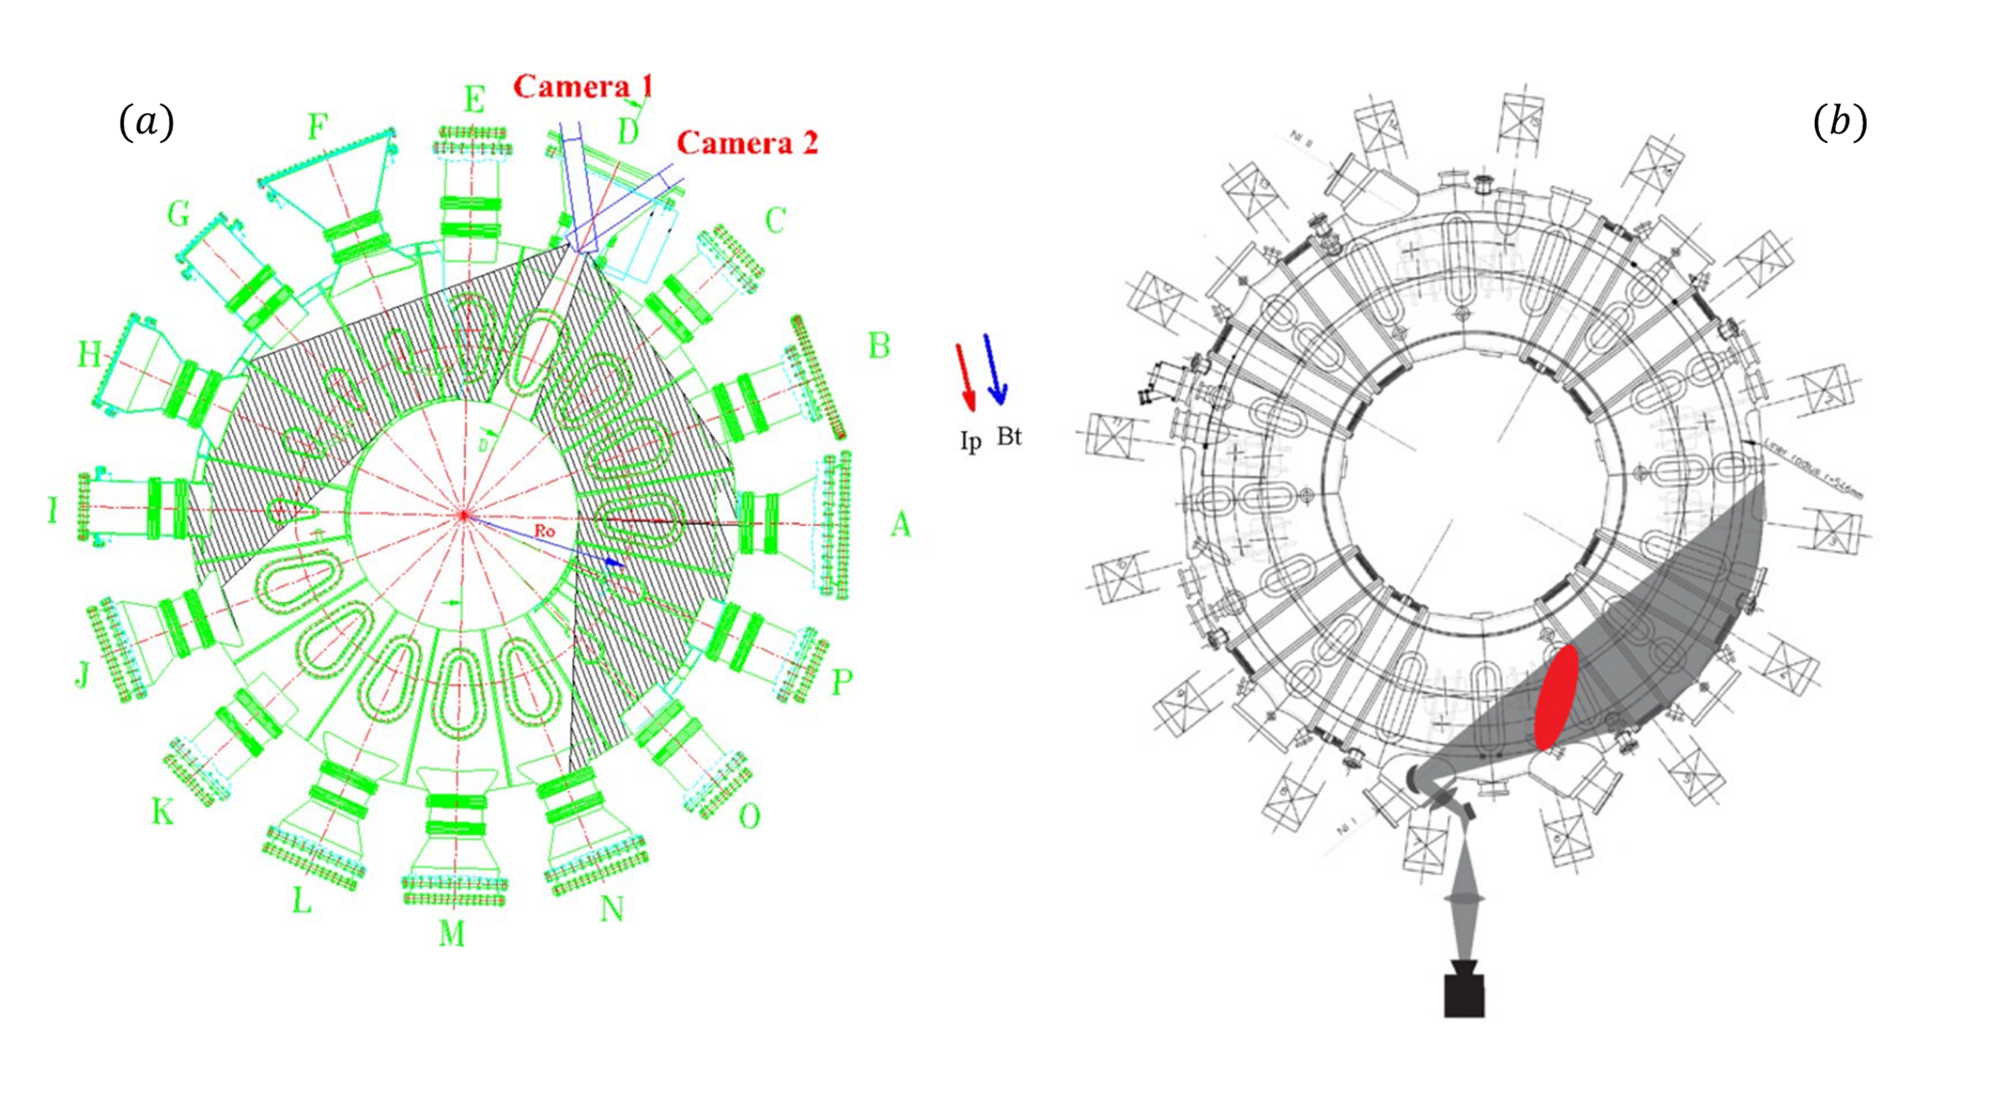
\includegraphics[width=12cm]{image45.png}
\caption{\label{fig:synchrotron2}(a)EAST装置可见光相机位置示意图\cite{RN1885}。(b)TEXTOR装置远红外相机示意图。灰色阴影区域表示接收光路区域\cite{RN1878}	}
\end{figure}
根据同步辐射方程\cite{RN1886},我们可以获得不同能量的逃逸电子对应的辐射波段。如\autoref{fig:synchrotron3}, 对于电子能量为25MeV的逃逸电子,同步辐射主要落在2-4um波段。结合同步辐射的定向性特征,可以通过沿托卡马克环向方向红外成像\cite{RN995,RN994,RN992}能获得逃逸电子的位置分布信息。\autoref{fig:synchrotron4}所展示的是EAST放电过程中不同时刻逃逸电子辐射光斑通过远红外相机成像\cite{RN1879}。
\begin{figure}[ht]
\centering
\includegraphics[width=14cm]{image46.png}
\caption{\label{fig:synchrotron3}不同逃逸电子能量的同步辐射谱\cite{RN1879}($R0=1.85$,$B_T=2T$,$v_⊥/v_∥ =0.05$)}
\end{figure}

\begin{figure}[ht]
\centering
\includegraphics[width=14cm]{image47.png}
\caption{\label{fig:synchrotron4}EAST放电不同时刻逃逸电子同步辐射通过远红外相机成像\cite{RN1879},(a)1.46s,(b)1.52s,(c)1.58s,(d)1.64s,(e)1.70s。}
\end{figure}
\clearpage
\subsection{	电子回旋辐射诊断}
电子回旋辐射诊断主要通过测量托卡马克等离子体中不同电子回旋频率的辐射信号来分析等离子体中电子温度分布(或涨落)。从技术路线上看主要有三种实现方式,分别是一维电子回旋辐射诊断(ECE)、二维电子回旋辐射成像诊断(ECEI)以及迈克尔逊干涉仪。其中ECE和ECEI在技术路线上方法基本一致,都是通过外差降频的方式实现对辐射信号的测量,只是相对ECE,ECEI拥有大尺度光学透镜,能够对等离子体直接成像,具有实现大尺度高时间空间分辨率优势。而迈克尔逊干涉仪则利用空间傅里叶分析实现对电子回旋辐射宽谱范围测量,频谱覆盖范围可从几十Ghz到几百Ghz,但时间分辨率只有ms量级\cite{RN743}。以ECEI系统为例,传统上用于ECEI诊断的电子回旋辐射需要满足3个条件:其一,电子回旋辐射需要保证能从等离子体中传出来,不能被反射和吸收;其二,电子回旋辐射需要满足光学厚条件,这样才能保证辐射强度和共振层温度正比关系,即黑体辐射条件;其三,电子辐射频率和托卡马克大半径位置要满足一一对应关系,也就意味着在观测区间内,电子回旋频率不能和其它谐波频率有重叠,一般情况下我们用二次X模可以满足这些条件。对于非热化电子,通常其产生条件是低密度等离子体环境,一般不满足光学厚条件。另一方面,在非热平衡条件下由于电子回旋辐射和$β_⊥$具有非线性关系,辐射变化强烈依赖于$β_⊥$值(\autoref{fig:etamax}),此时超热电子的回旋辐射强度远大于背景热电子的回旋辐射强度,电子回旋辐射信号的分析就需要结合计算机模拟和其它诊断完成。通过结合低时间分辨宽频测量的迈克尔逊干涉仪和大尺度高时间空间分辨的电子回旋辐射诊断可以互相弥补不足,获得更多有效信息。在D.J. Campbell\cite{RN726}的工作里有两者结合的经典实验研究,简要介绍如下:
\begin{figure}[ht]
\centering
\includegraphics[width=15cm]{image48_1.png}
\caption{\label{fig:ECEspec}从热等离子体到非热等离子体演化过程中电子回旋辐射特征图\cite{RN726}。(a) 线平均等离子体密度$n_e$和表示为等效温度的2$ω_{ce} (0)-X$模电子回旋辐射强度。(b)标签a-e时刻测量得到的电子回旋辐射谱分布。(c)利用双能分布模拟得到辐射谱分布,其中包括低能部分(LE)和高能部分(HE),低能部分为热分布,高能部分为超热分布,通过改变分布函数密度和能量拟合辐射谱形状}
\end{figure}

在低密度放电条件下(通常指$ω_{pe}/ω_{ce} <1$,其中$ω_{pe}$表示电子等离
子频率,$ω_{ce}$表示电子回旋频率),由于电子之间碰撞频率降低,电子在电
场驱动下易形成偏离热分布的非热化电子。如果对分布函数采用一定的简化形
式,使得辐射谱形状能够通过有限的分布参数拟合获得,这样根据辐射谱的形状研究非热化电子就具备一定的可行性。其中一个分布函数简化方法就是双能分
布,将分布函数分为高能部分和低能部分,低能部分对应主体等离子体的密度和温度,用麦氏分布描述。高能部分主要对应偏离主体分布的非热化电子。通过对高能
部分采用不同分布函数形式计算发现:当垂直方向平均能量超过30keV后,对于不同的高能电子分布形式,只要密度和垂直方向平均能量相同,辐射谱的形状就没有明显差别。D.J. Campbell\cite{RN726}对这种现象的解释是高于$3ω_{ce}$辐射频率部分由于
各谐波分量之间相互重叠导致结构平滑,不能反映分布函数的细节。在平均能量
相同的前提下,谱的形状对分布函数并不敏感。因此高能部分可以采用相对论麦
氏分布模型表示,这样就可以根据高能部分和低能部分的密度和平均能量唯一的拟合出辐射谱结构。
\par 根据这个方法,1984年D.J. Campbell分别利用快速迈克尔逊干涉仪和多色仪测量了ASDEX托卡马克装置上非热化电子辐射[139]。迈克尔逊干涉仪通过15ms空间傅里叶变换得到$ω_{ce} (0)-5ω_{ce} (0)$区间的电子回旋辐射谱(这里$ω_{ce} (0)$表示磁轴位置处电子回旋频率),而多色仪利用光栅可以实现单频率高时间分辨测量,这两种诊断的视角均在托卡马克中平面沿着径向方向。除此之外,还有汤姆逊散射系统用于监测等离子体热电子密度和热电子温度。为了获得低密度放电条件,通常在正常的放电下($B_T (0)=2.2T$,$I_p=250-350kA$,$n_e=(2-3)×10^{13} cm^{-3}$,$T_e=600-700eV)$通过控制注入$D_2$气体,将等离子体密度降低到设定的值(通常是$(2-3)×10^{12} cm^{-3}$)。如\autoref{fig:ECEspec}所示,当在0.7s关闭气体注入时,随着等离子体密度下降至低密度平台区间,等离子体芯部ECE信号稳定上升然后在1.07s时突然升高并导致信号饱和。a-e时刻对应电子回旋辐射谱如\autoref{fig:ECEspec}(b)所示。根据双能分布模型,其中低能电子密度和能量由实验测量获得,通过拟合即可得到a-e过程中高能部分电子密度和垂直方向平均能量,如\autoref{fig:ECEspec}(c)。关于在1.07s处为什么会突然上升,Campbell没有详细的展开研究,只是猜测可能是反常多普勒效应导致速度出现散射,本文在\autoref{sec:exp_ece}也对类似的这种现象展开讨论,并得到了与之不同的结论。\par
D.J. Campbell 的方虽然可以实现对非热化电子数量和能量的拟合,但是由于其诊断视角在中平面沿着半径方向,纵场的变化也一定会对谱分布结构带来影响,因此1990年G.Taylor采用垂直方向接收电子回旋辐射谱\cite{RN2037}。如\autoref{fig:VECE}所示,该诊断可以通过调节反射镜实现三个不同径向位置垂直方向电子回旋辐射测量,由于垂直方向纵场几乎不变,因此可以获得固定纵场条件下的电子回旋辐射谱,然后使用双温分布拟合电子回旋辐射谱获得非热化电子的平均能量和数量。通过垂直方向测量电子回旋谱分布的另一个直观的优点是可以根据辐射频率估算高能电子能量,这是因为当地电子回旋频率会由于相对论效应出现展宽,通过测量不同能量对应辐射频率的强度原则上就能研究非热化电子能量分布。但是实际上由于壁面反射导致测量信号并不一定来自对应测量径向位置通道的信号,实验中还是有很多需要考虑的问题,例如评估壁反射对信号的污染,如何抑制壁反射等。 M. Farník在研究COMPASS托卡马克上逃逸电子回旋辐射时对此有过详细的分析\cite{RN823}。
\begin{figure}[ht]
\centering
\includegraphics[width=12cm]{image49_1.png}
\caption{\label{fig:VECE}TFTR垂直方向电子回旋辐射诊断\cite{RN2037}}
\end{figure}
  \par 尽管双能分布简化了分布函数的复杂度,但不免会丢失很多细节上的信息。如果能建立分布函数演化模型,计算不同时刻下分布函数形状和电子回旋谱信号,同时结合实验过程中用到的电子回旋辐射诊断,对比模拟辐射信号和实验中观测到的辐射信号,这将会对非热化电子辐射以及其背后的物理过程有更加直观的理解。为了实现这个目的,在接下来的章节中本文将依次介绍不同速度分布下电子回旋辐射信号的计算以及电子速度分布演化的数值模拟方法,为实验测量所得辐射结构提供数值研究平台。
\section{小结}
本章给出了等离子体中电子速度分布函数的动理学模型以及探测非热化电子的
相关诊断方法。在非热化电子的动理学模型中,本章讨论了小角度散射的Fokker-Planck碰撞算符$C[f]$、雪崩算符$S_A[f]$、辐射阻尼算符$\frac{\partial}{\partial \boldsymbol{p}} \cdot\left(F_{\mathrm{rad}} f\right)$、电场驱动算符以及准线性扩散算符$D[f]$等。非热电子理论将用于动理学计算程序中,以实现非热电子演化的数值模拟。关于非热电子诊断方面主要介绍了同步辐射诊断,轫致辐射诊断以及电子回旋辐射诊断。为了将电子速度分布演化过程与实验诊断数据相互比较,在下一章中我们主要研究电子回旋辐射诊断的数值模拟平台,解决任意电子速度分布映射到电子回旋辐射的正向过程,进而实现与实验现象中电子回旋辐射信号的直接对比,这样我们的模拟数据就有了实验参考,而不是脱轨的数值幻象。 


















%!TeX root = ../main.tex
\chapter{电子回旋辐射数值诊断}
\section*{引言}
%电子回旋辐射在等离子体中伴随着吸收和发射过程。等离子体若发射某一频率的辐射,也必将吸收同一频率的辐射。对于有辐射和吸收的等离子体,根据能量守恒条件,辐射输运方程可表示为
电子回旋辐射在输运中伴随着吸收和发射过程。介质若发射某一频率的辐
射,也必将吸收同一频率的辐射,因此介质对辐射输运过程起到重要作用。根据
基尔霍夫定律,辐射输运方程为
\begin{equation}
\mathrm{N}^{2} \frac{d}{d s}\left(\frac{\mathrm{I}}{\mathrm{N}^{2}}\right)=\eta_{\omega}-\alpha_{\omega} I
\end{equation}
其中$η_\omega$表示体辐射率,它表示单位体积等离子体沿入射辐射方向单位立体角的辐射功率,$α_\omega$表示体辐射吸收系数,N表示等离子体的折射率。在稀薄等离子体近似条件下,$N≈1$,这时辐射方程为
\begin{equation}\label{eq:dids}
\frac{d I}{d s}=\eta_{w}-\alpha_{w} I
\end{equation}
可见最终电子回旋辐射信号强度取决于路径s,等离子体辐射率$η_\omega$以及吸收系数$α_\omega$等。\par
本章主要目的是解决稀薄等离子体电子回旋辐射的计算问题,从单电子回旋辐射出发,计算等离子体辐射率$η_\omega$。接着着力解决辐射输运问题,包括射线追迹s、辐射吸收系数$α_\omega$等,最终建立完整的信号流程,为非热化电子动理学演化过程中电子回旋辐射提供数值诊断计算平台。
\section{等离子体辐射率}
在稀薄等离子体中$ω_{pe}/ω_{ce} ≪1$,等离子体自身的折射率接近于真空折射率,此时可以忽略折射率和电子-电子运动耦合对辐射的影响,等离子体电子回旋辐射可以通过单电子回旋辐射统计求和的方式给出\cite{RN1898}。本章所有计算都是在这一默认前提下完成。
\subsection{单电子回旋辐射}
如\autoref{fig:elecorb}所示,均匀磁场背景中,单电子绕磁力线螺旋运动产生的单位时间单位频率单位立体角的辐射谱可以表示为(见附录\autoref{sec:A1}):
\begin{equation}\label{eq:nw}
\eta_{1}(\omega, v, \theta)=\frac{e^{2} \omega^{2}}{8 \pi^{2} \varepsilon_{0} c} \sum_{1}^{\infty}\left|\begin{array}{c}-\hat{\mathrm{x}} \frac{\cos \theta}{\sin \theta}\left(\cos \theta-\beta_{\|}\right) J_{m}(\xi) \\-\hat{y} j \beta_{\perp} \frac{d J_{m}(\xi)}{d \xi} \\\hat{\mathrm{z}}\left(\cos \theta-\beta_{\|}\right) J_{m}(\xi)\end{array}\right|^{2} \delta\left[\left(1-\beta_{\|} \cos \theta\right) \omega-m \omega_{c e}\right]
\end{equation}
取模算符中向量$\hat{x}$、$\hat{y}$、$\hat{z}$表示辐射电磁波的偏振方向,$θ$表示观测方向和磁场方向的夹角。当$θ=π/2$时,电磁波的传播模式可分为X波和O波,其中X波电场振动方向垂直于磁场和传播方向($\hat{y}$方向),O波电场振动方向平行于磁场方向($\hat{z}$ 方向)。$\hat{q}$为传播方向,平行于$\hat{q}$方向的电场具有纵波特征。当$θ≠π/2$时,具有类似O、X波极化方向的电磁波对应功率分别表示为:
\begin{subequations}\label{eq:etapp}
\begin{align}
\eta_{1}^{\|}(\omega, \beta, \theta)&=\frac{e^{2} \omega^{2}}{8 \pi^{2} \varepsilon_{0} c}\sum_{1}^{\infty}\left|\hat{\mathrm{z}}\left(\cos \theta-\beta_{\|}\right) J_{m}(\xi)\right|^{2} \delta\left[\left(1-\beta_{\|} \cos \theta\right) \omega-m \omega_{c e}\right]\\
\eta_{1}^{\perp}(\omega, \beta, \theta)&=\frac{e^{2} \omega^{2}}{8 \pi^{2} \varepsilon_{0} c}\sum_{1}^{\infty}\left|-\hat{y} j \beta_{\perp} \frac{d J_{m}(\xi)}{d \xi}\right|^{2} \delta\left[\left(1-\beta_{\|} \cos \theta\right) \omega-m \omega_{c e}\right]
\end{align}
\end{subequations}

其中$∥(⊥)$表示电场平行(垂直)于磁场的电磁波。考虑所有偏振方向,总辐射功率为:
\begin{equation}
\eta_{1}(\omega, v, \theta)=\frac{e^{2} \omega^{2}}{8 \pi^{2} \epsilon_{0} c}  \sum_{1}^{\infty}\left[\begin{array}{c}\left(\frac{\cos \theta-\beta_{\|}}{\sin \theta}\right)^{2} J_{m}^{2}(\xi) \\+\beta_{\perp}^{2} J_{m}^{\prime2}(\xi)\end{array}\right] \delta\left[\left(1-\beta_{\|} \cos \theta\right) \omega-m \omega_{c e}\right]
\end{equation}
其中$J_m$表示第一类m阶贝塞尔函数,$ξ=(ωβ_⊥)/ω_{ce} sinθ$,$ω_{ce}=\frac{eB_0}{γm_e} $。
\begin{figure}[ht]
\centering
\includegraphics[width=12cm]{image50.png}
\caption{\label{fig:elecorb}均匀磁场中电子螺旋运动图}
\end{figure}
由\autoref{eq:nw}可知电子回旋辐射谱是由m=1、2、3…..一系列δ函数分立谱组成,即理论上电子回旋辐射是有无穷个谐频谱组成,对应的谐频频率为: 
\begin{equation}\label{eq:resonant}
\omega=\frac{m \omega_{\mathrm{ce}}}{1-\beta_{\|} \cos \theta}=\frac{{m \omega_{\mathrm{c} 0}}/{\gamma}}{1-\beta_{\|} \cos \theta}
\end{equation}
其中分母$(1-β_∥ cosθ)$和多普勒频移有关,$γ$和相对论频移有关。由于电子具有一定的速度分布,因此对于任一固定的 m 
次谐频,它都会有一定的频率展宽,称之为共振层,在该共振层内辐射频率、电子速度满足
\begin{equation}
\left(1-\beta_{\|} \cos \theta\right) \omega-m \omega_{c e}=0
\end{equation}
对于ECEI,理论上接收方向垂直于纵向磁场,取$θ=π/2$,这时候共振层主要依赖于相对论效应。考虑电子回旋基频为45GHz,对于85Ghz的辐射信号,其2、3、4次谐频共振曲线如\autoref{fig:resonant}所示,不同谐波共振层都是标准圆,谐波次数越高,圆半径越大,满足共振层条件的电子所需能量越高。但是限于空间条件或实验要求,接收方向和磁场方向夹角并不一定是严格90度,为了更加直观,这里取夹角$θ=π/3$,得到如\autoref{fig:resonant}所示的虚线,由于多普勒效应出现,共振曲线变成了椭圆。共振意味着波和粒子可以发生强烈的相互作用,比如外部入射的电磁波可以把能量传递给相应的粒子,因此根据椭圆共振层特征还可以实现等离子体平行方向电子速度分布测量。例如对于$f_{ce}/f\sim1$的微波信号以$cosθ=0.4(N_∥=0.4)$角度穿过处在匀强磁场中的等离子体,如\autoref{fig:resonant2}所示,当电子能量E<200keV时,垂直磁场方向温度$T_e<10keV$,对于不同的频率可认为只有唯一的$p_∥$与之发生共振。此时吸收系数完全由平行方向速度分布函数确定,通过测量不同频率信号的透射率就可以实现平行方向速度分布诊断\cite{RN1413}。
\begin{figure}[ht]
\centering
\includegraphics[width=12cm]{image51.png}
\caption{\label{fig:resonant}基频$ω_{c0}=45GHz$,辐射频率$ω=85GHz$,传播方向垂直于磁场(实线)和与磁场夹角$θ=π/3$(虚线)时不同谐波的共振层形状}
\end{figure}
\begin{figure}[ht]
\centering
\includegraphics[width=12cm]{image52.png}
\caption{\label{fig:resonant2}不同频率下 $N_∥=0$(黑色虚线)和$N_∥=0.4$(黑色实线)共振曲线,其中$p_⊥ $、$p_∥ $表示约化动量,约化因子为$m_e c$ ,蓝色虚线对应垂直方向温度为10$keV$时所对应的平均垂直动量}
\end{figure}
\subsection{磁化等离子体电子回旋辐射}
当等离子体足够稀薄,自由空间处理是适用的,同时假设各个电子的辐射是不相关的,我们只需要对所有单个电子辐射强度简单求和从而获得等离子体的发射率。考虑归一化分布函数为$f(β_∥,β_⊥ )$,密度为$n_0$的等离子体,等离子体辐射率则表示为
\begin{equation}\label{eq:etawint}
\eta_{\omega}=n_{0} c^{3} \iint \eta_{1}  2 \pi \beta_{\perp} f\left(\beta_{\|}, \beta_{\perp}\right) d \beta_{\perp} d \beta_{\|}
\end{equation}
由\autoref{eq:etapp}和\autoref{eq:etawint}得:
\begin{equation}
\begin{aligned}\eta_{\mathrm{w}}^{\perp, \|}=n_{0} c^{3} & \sum_{m=1}^{+\infty} \iint d \beta_{\perp} d \beta_{\|}  \\& \times Q^{\perp, \|} \delta\left[\left(1-\beta_{\|} \cos \theta\right) \omega-m \omega_{c e}\right] \cdot 2 \pi \beta_{\perp} f\left(\beta_{\|}, \beta_{\perp}\right)\end{aligned}
\end{equation}
其中$Q^{(⊥,∥)}$分别为
\begin{subequations}
\begin{align}
Q^{\perp} & = \frac{e^{2} \omega^{2}}{8 \pi^{2} \epsilon_{0} c}\left[\beta_{\perp}^{2} J_{m}^{\prime 2}(\xi)\right] \\
Q^{\|} & = \frac{e^{2} \omega^{2}}{8 \pi^{2} \epsilon_{0} c}\left[\hat{\mathrm{z}}\left(\cos \theta-\beta_{\|}\right) J_{m}(\xi)\right]^{2}
\end{align}
\end{subequations}
这里$Q^⊥$ 、$Q^∥$分别表示电场方向垂直和平行于背景磁场的电磁波辐射算符(即X波和O波) 。辐射展宽的机制主要有两类,分别为相对论展宽$(1-β^2 )^{1/2}$和多普勒展宽$(1-β_∥ cosθ)^{-1}$。除此之外还有由于辐射导致电子能量指数衰减的自然展宽以及碰撞导致的碰撞展宽,相对于前两种展宽,之后的两种展宽可以忽略不计\cite{RN1900}。求解积分主要困难来自于积分项中二维狄拉克函数,解决方式是把二维积分通过狄拉克函数的性质转化为一维积分,具体方法可参考附录\autoref{sec:A3}。\par
  这里为了展示热分别状态下辐射率的频谱分布,假设等离子体速度分布为各项同性且满足麦氏分布,不考虑相对效应,分布函数可表示为:
\begin{equation}
f\left(\beta_{\|}, \beta_{\perp}\right)=\left(\frac{m_{e}}{2 \pi T}\right)^{\left(\frac{3}{2}\right)} \exp \left[\frac{m_{e} c^{2}\left(\beta_{\perp}^{2}+\beta_{\|}^{2}\right)}{2 T}\right]
\end{equation}\par
考虑ECEI接收到的电磁波为X模,且垂直纵场方向,取$Q=Q^⊥$,$θ=π/2$,$T=5~keV$, $n_e=10^{19}~m^{-3}$,根据$η_\omega^⊥$计算可得辐射频谱如\autoref{fig:spece}所示,信号强度主要集中在基频和二次谐频上,且谐频分布彼此重叠较小,更高次谐频之间相互重叠区域较大,分辨度小,且强度较低。因此电子回旋辐射诊断主要选取基频和二次谐频,保证了信号强度号和谐频成分的单一性。同时为了保证信号能传出托卡马克,对于X模通常选择二次谐频,对于O模通常选取基频(可参考\autoref{sec:ECEI})。
\begin{figure}
\centering
\includegraphics[width=14cm]{image53.png}
\caption{\label{fig:spece}温度为5keV,$f_{c0}=50GHz$,$n_e=10^{19}/m^3$时电子回旋辐射频谱图}

\end{figure}
\clearpage
\section{等离子体吸收系数}
\subsection{局部热平衡态下等离子体吸收系数}
当等离子体处于温度为$T_e$的局部热平衡态,单位路径吸收的电磁波能量和辐射的能量达到动态平衡。根据基尔霍夫定理,有
\begin{equation}
\eta_{\omega}-\alpha_{\omega} I_B=0
\end{equation}
吸收系数为
\begin{equation}\label{eq:alphaT}
\alpha_{\omega}=\frac{\eta_{\omega}}{I_B}
\end{equation}
普朗克黑体辐射表面亮度$I_B$(单位面积单位立体角辐射功率)可表示为
\begin{equation}
\mathrm{I}_{B}(\omega)=\frac{\hbar \omega^{3}}{4 \pi^{3} c^{2}} \frac{1}{e^{\frac{\hbar \omega}{T_{e}}}-1}
\end{equation}
考虑$ℏω≪T_e$,泰勒展开取一阶量得到
\begin{equation}\label{eq:Black}
\mathrm{I}_{B}(\omega)=\frac{T_{e} \omega^{2}}{4 \pi^{3} c^{2}}
\end{equation}
因此在满足黑体条件下辐射强度正比与温度,进一步考虑线偏振电磁波,如X模或O模,$I_B$则为
\begin{equation}
\mathrm{I}_{B}(\omega)=\frac{T_{e} \omega^{2}}{4 \pi^{3} c^{2}} * \frac{1}{2}=\frac{T_{e} \omega^{2}}{8 \pi^{3} c^{2}}
\end{equation}
最终,在热平衡条件下,根据\autoref{eq:alphaT}等离子体吸收系数为:
\begin{equation}\label{eq:alphaT2}
\alpha_{\omega}=\eta_{\omega} * \frac{8 \pi^{3} c^{2}}{T_{e} \omega^{2}}
\end{equation}

\subsection{非热平衡态下等离子体吸收系数}
在上一小节中主要考虑的是热平衡条件下(电子速度分布满足麦克斯韦分布)等离子体吸收系数的计算,吸收系数$α_ω$根据发射系数通过基尔霍夫定律求得:$α_ω=η_ω/I_B $。如果电子速度分布不满足热平衡条件时,吸收系数的计算需要通过更精细的能量平衡方程求得。\par
首先假设等离子体的折射率n$\sim$1,辐射能量输运方程表达式:
\begin{equation}
\frac{\partial \mathrm{I}_{\omega}^{\mathrm{i}}}{\partial \mathrm{s}}=\eta_{\omega}^{i}-\alpha_{\omega}^{i} I_{\omega}^{i}
\end{equation}
i表示极化类型,这里$η_\omega^i$和$α_\omega^i$分别为
\begin{align}\eta_{\omega}^{\mathrm{i}} & = \int \eta_{1}^{i}(\boldsymbol{p}) f(\boldsymbol{p}) d \boldsymbol{p} \\ \alpha_{\omega}^{\mathrm{i}} & = \int \alpha_{1}^{i}(\boldsymbol{p}) f(\boldsymbol{p}) d \boldsymbol{p}
\end{align}
这里$ η_1^i (p)$ 表示单电子自发辐射率,如磁化等离子体中的\autoref{eq:nw},$α_1^i (p)$表示运动状态为$\vp$的电子吸收系数。根据光子的量子性特征,动量为$\vp'$态的电子辐射出一个光子后变成$\vp$态,根据动量守恒和能量守恒关系 : 
\begin{align}
\boldsymbol{p}_{\|} & = \boldsymbol{p}_{\|}^{\prime}-\hbar \boldsymbol{k}_{\|}\\ \epsilon & = \epsilon^{\prime}-\hbar \omega
\end{align}
其中$∥$表示与磁场方向平行,电子通过在平行磁场方向失去(获得)动量而发射(吸收)光子。动量为$\vp'$电子的受激发射系数$\chi_1^{i*}({p} \prime)$和受激发射率$\eta_1^{i*}({p} \prime)$之间满足关系$\eta_1^{i*}({p} \prime)=\chi_1^{i*}({p} \prime)I_{\omega}$,$I_{\omega}$为背景辐射强度。根据爱因斯坦系数关系,受激发射系数$\chi_1^{i*} (\vp' )$和自发发射率$η_1^{i} (\vp' )$满足\cite{RN1002,RN2117}:
\begin{equation}
\eta_{1}^{i}\left(\boldsymbol{p}^{\prime}\right)=\chi_{1}^{i *}\left(\boldsymbol{p}^{\prime}\right) \frac{\hbar \omega^{3}}{8 \pi^{3} c^{2}}
\end{equation}
动量为$\vp$电子的受激吸收系数和动量为$\vp'$电子的受激发射系数之间的关系满足
\begin{equation}
\alpha_{1}^{i *}(\boldsymbol{p})=\frac{\Omega_{{p} \prime}}{\Omega_{{p}}} \chi_{1}^{i *}\left(\boldsymbol{p}^{\prime}\right)
\end{equation}
$Ω_\vp$,$Ω_\vp'$分别表示动量$\vp$和$\vp'$状态的统计权重且$Ω_\vp'/Ω_\vp=\dif\vp'/\dif\vp$。
根据以上方程,辐射能量输运方程可表示为:
\begin{equation}
\begin{aligned}
\frac{\partial I_{\omega}}{\partial s} & =\int f\left(\boldsymbol{p}^{\prime}\right)\left[\eta_{1}^{i}\left(\boldsymbol{p}^{\prime}\right)+\eta_{1}^{*}\left(\boldsymbol{p}^{\prime}\right)\right] d \boldsymbol{p}^{\prime}-I_{w} \int f(\boldsymbol{p}) \alpha_{1}^{*}(\boldsymbol{p}) d \boldsymbol{p}  \\
& =\int f\left(\boldsymbol{p}^{\prime}\right) \eta_{1}^{i}\left(\boldsymbol{p}^{\prime}\right) d \boldsymbol{p}^{\prime}-I_{w} \frac{8 \pi^{3} c^{2}}{w^{2}} \int \eta_{1}^{i}\left(\boldsymbol{p}^{\prime}\right) \frac{\left[f(\boldsymbol{p})-f\left(\boldsymbol{p}^{\prime}\right)\right]}{\hbar w} d \boldsymbol{p}^{\prime} \\
& =\eta_{\omega}^{i}-I_{\omega} \alpha_{w}^{i} 
\end{aligned}
\end{equation}
其中
\begin{align}
\eta_{{\omega}}^{i} & = \int f\left(\boldsymbol{p}^{\prime}\right) \eta_{1}^{i}\left(\boldsymbol{p}^{\prime}\right) d \boldsymbol{p}^{\prime} \\
\alpha_{\omega}^{i} & = \frac{8 \pi^{3} c^{2}}{\omega^{2}} \int \eta_{1}^{i}\left(\boldsymbol{p}^{\prime}\right) \frac{\left[f(\boldsymbol{p})-f\left(\boldsymbol{p}^{\prime}\right)\right]}{\hbar \omega} d \boldsymbol{p}^{\prime}\label{eq:alpha1}
\end{align}
为了研究$α_\omega^i$,首先需要把$α_\omega^i$表示成数学可以处理的形式,不难发现
\begin{equation}\label{eq:fte}
f\left(\boldsymbol{p}^{\prime}\right)=f\left(\boldsymbol{p}_{\|}^{\prime}, \epsilon^{\prime}\right)=f\left(\boldsymbol{p}_{\|}+\frac{\hbar \omega}{c} \cos \theta, \epsilon+\hbar \omega\right)
\end{equation}
由于辐射出光子的动量远小于电子本身动量$(ℏk\ll \vp')$,辐射出的光子能量远小于电子本身携带的能量$(ℏω\ll ϵ')$,因此$f(\vp' )$可表示为一阶泰勒展开形式,
由\autoref{eq:alpha1}和\autoref{eq:fte}得:
\begin{equation}\label{eq:alpha2}
\alpha_{\omega}=-\frac{8 \pi^{3} c^{2}}{\omega^{2}} \int \eta_{1}^{i}\left(\boldsymbol{p}^{\prime}\right) \left[\frac{\partial f}{\partial p_{\|}} \cdot \frac{\cos \theta}{c}+\frac{\partial f}{\partial \epsilon}\right]\dif {\vp}^{\prime}
\end{equation}
根据文献记载,该方程最早由前苏联科学家TRUBNIKOV推导得到\cite{RN1344}。为了计算方便,本文中将积分坐标从$(p_∥,ϵ)$转化为$(p,ξ)$,其中p是约化因子为$m_ec$的约化动量,$\xi=p_{\|}/p$,最终形式为(可参考附录\autoref{sec:A2})
\begin{equation}
\alpha_{\omega}=-\frac{8n_{0} \pi^{3} c^{2}}{m_{e} c^{2} \omega^{2}} \int \eta_{1}^{i}(\beta, \xi)\left[\frac{1}{p} \frac{\partial f}{\partial \xi} \cos \theta+\frac{\sqrt{1+p^{2}}}{p} \frac{\partial f}{\partial p}-\frac{\xi \sqrt{1+p^{2}}}{p^{2}} \frac{\partial f}{\partial \xi}\right] 2 \pi p^{2}  \dif p \dif \xi
\end{equation}
当$ θ=π/2$,且分布函数满足麦克斯韦分布即$ f\sim \exp(-ϵ/T_e )$,由\autoref{eq:alpha2}得:
\begin{equation}
\alpha_{\omega}=\eta_{\omega} * \frac{8 \pi^{3} c^{2}}{T_{e} \omega^{2}}
\end{equation}
此时吸收系数退回到热平衡态的\autoref{eq:alphaT2}。\par
当等离子体满足热平衡条件时,光学厚度是决定辐射强度和温度关系的一个重要指标,根据等离子体输运方程\autoref{eq:dids},在不考虑壁反射条件下,最终接收到的信号强度满足方程:
\begin{equation}
I(s)=\frac{\eta_{\omega}}{\alpha_{\omega}}\left[1-e^{-\tau}\right]
\end{equation}
其中光学厚度的定义为
\begin{equation} \label{eq:tauN}
τ=∫α_\omega \dif s
\end{equation}
在满足局部热平衡条件时,根据\autoref{eq:alphaT2}
\begin{equation}
\frac{\eta_{\omega}}{\alpha_{\omega}}=I_{B}(T) \sim \frac{T_{e} \omega^{2}}{8 \pi^{3} c^{2}}
\end{equation}
因此只有当光学厚度$τ>1$时辐射强度才近似正比于温度$T_e$。
\subsection{两种光学厚度计算方法的对比}
本论文之后的吸收系数计算均采用上述利用爱因斯坦系数关系得到的\autoref{eq:alpha2}。我们将之与经典的局域热平衡等离子体光学厚度计算方法\cite{RN1952}进行进一步校验。以EAST托卡马克参数为环境背景,其大半径R0=1.85m,小半径a=0.45m。假设放电中纵场电流为IT=10000A,对应磁轴处磁场强度大约为2.25T。我们考虑两种密度分布环境,分别为低密度环境,对应磁轴中心密度为$n_{ea0}=7\times10^{18}m^{-3}$,以及高密度环境,对应磁轴中心密度为$n_{eb0}=3\times10^{19}m^{-3}$,芯部温度均为$T_{e0}=1keV$,进一步假设密度分布和温度分布满足二次分布:
\begin{align}
n_{e r} & =n_{e 0} \left(1-\rho^{2}\right)^{2} \label{eq:nr}\\
T_{e r} & =T_{e 0} \left(1-\rho^{2}\right)^{2}\label{eq:Tr}
\end{align}
其中$\rho$表示约化半径,$ρ<0$对应高场侧,$ρ>0$对应低场侧。我们通过计算不同半径处所对应的冷等离子体二次回旋频率光学厚度来对两种计算方法进行比较。\\
\noindent 1.通过爱因斯坦发射吸收系数计算光学厚度\par
利用Trubnikov\autoref{eq:alpha2}计算二次电子回旋频率在不同位置处吸收系数的分布,最后通过数值的方法计算吸收系数沿光学路径的积分,从而获得不同半径冷等离子体电子回旋频率对应的光学厚度。这里选择直线为积分路径,没有考虑等离子体的折射效应。\par
\noindent 2.从等离子体介电属性出发解析计算光学厚度\par
另一种求解吸收系数的方式是通过电磁波在等离子体中传播的能量输运方程,利用输运方程中单位路径的能量的吸收和能流之比来求解吸收系数,吸收系数可表示为\cite{RN1952}
\begin{equation}\label{eq:alphaBornatic}
\alpha=\left[(\omega / 4 \pi) \overrightarrow{\widetilde{E}}^{*} \cdot \overrightarrow{\varepsilon_{a}} \cdot \overrightarrow{\tilde{E}}\right] /|\vec{S}|
\end{equation}
其中
\begin{equation}
\vec{S}\left(\vec{k}^{\prime}, \omega\right) \equiv \frac{c}{4 \pi} \operatorname{Re}\left(\overrightarrow{\widetilde{E}} \times \vec{\widetilde{B}}^{*}\right)-\frac{\omega}{8 \pi} \frac{\partial \varepsilon_{h, i j}}{\partial \vec{k}^{\prime}} \widetilde{E}_{i}^{*} \tilde{E}_{j}
\end{equation}
$\overrightarrow{\widetilde{E}} $和$\vec{\widetilde{B}}$表示电磁波的电场和磁场,$\omega$为电磁波角频率,$\varepsilon_{h, i j}$和$\varepsilon_{a, i j}$分别为等离子体的实介电张量和虚介电张量,与分布函数的具体形式有关,$\vec{k}^{\prime}$为电磁波波矢。\autoref{eq:alphaBornatic}中分子表示等离子体对电磁波的吸收,分母表示能流。在满足局部热平衡条件下Bornatici根据\autoref{eq:alphaBornatic}推导出托卡马克中n次回旋频率$(n≥2)$光学厚度的计算公式如下\cite{RN351}:
\begin{equation}\label{eq:tauB}
\tau_{n}^{(X,O)}(\theta)=\frac{\pi n^{2(n-1)}}{2^{n}(n-1) !}\left(\frac{\omega_{p}}{\omega_{c}}\right)^{2}\left(\frac{T}{m_e c^{2}}\right)^{n-1}(\sin \theta)^{2(n-1)}\left(1+\cos ^{2} \theta\right) \mu_{n}^{(x, 0)}(\theta) \frac{\omega_{c} L_{B}}{c}
\end{equation}
其中$ω_p$表示等离子体频率,$ω_c$表示电子回旋频率、T表示等离子体温度,$L_B=\left(\frac{1}{B_{0}} \frac{\partial B_{0}}{\partial s}\right)^{-1}$表示纵场(纵向磁场)梯度标长,$θ$表示传播方向和背景磁场的夹角,$μ_n^{(X,O) }$定义为:
\begin{equation}
\mu_{n}^{(X, O)}(\theta) \equiv \frac{\left(N^{(x, 0)}\right)^{2 n-3}}{1+\cos ^{2} \theta} \frac{(n-1)^{2}\left[1-\left(n+\frac{1}{n}\right) f_{n}^{(X, O)}(\theta)\right]^{2}}{\left[\left(a_{n}^{2}+b_{n}^{2}\right)^{\frac{1}{2}}\right]_{N=N^{(X, O)}}}
\end{equation}
$a_n$和$b_n$的定义为:
\begin{align}
a_{n}^{2}& \equiv\left[1+\frac{\left[1-\left(\frac{\omega_{p}}{n \omega_{c}}\right)^{2}\right] N^{2} \cos ^{2} \theta}{\left[1-\left(\frac{\omega_{p}}{n \omega_{c}}\right)^{2}-N^{2} \sin ^{2} \theta\right]^{2}} n^{2}\left(1-\frac{n^{2}-1}{n^{2}} f_{n}^{(\mathrm{x}, \mathrm{o})}\right)^{2}\right]^{2} \sin ^{2} \theta \\
b_{n}^{2} &\equiv\left[1+\frac{1-\left(\frac{\omega_{p}}{n \omega_{c}}\right)^{2}}{1-\left(\frac{\omega_{p}}{n \omega_{c}}\right)^{2}-N^{2} \sin ^{2} \theta} n^{2}\left(1-\frac{n^{2}-1}{n^{2}} f_{n}^{(x, 0)}\right)^{2}\right]^{2} \cos ^{2} \theta
\end{align}
$N^2=\left [N^{(X,O)} \right]^2$和$f_n^{(X,O) }$的定义为:
\begin{align}
\left[N^{(X, O)}\right]^{2} = 1-\left(\frac{\omega_{p}}{n \omega_{c}}\right)^{2}& \frac{2\left[n^{2}-\left(\frac{\omega_{p}}{\omega_{c}}\right)^{2}\right]}{2\left[n^{2}-\left(\frac{\omega_{p}}{\omega_{c}}\right)^{2}\right]-\sin ^{2} \theta \mp  
\rho_{n}} \equiv 1-\left(\frac{\omega_{p}}{n \omega_{c}}\right)^{2} f_{n}^{(X, 0)}(\theta) \\
\rho_{n}^{2} \equiv \sin ^{4} &\theta+\frac{4}{n^{2}}\left[n^{2}-\left(\frac{\omega_{p}}{\omega_{c}}\right)^{2}\right]^{2} \cos ^{2} \theta
\end{align}
其中+表示X波,-表示O波。
\begin{figure}[H]
\centering
\includegraphics[width=14cm]{image55_2.eps}
\caption{\label{fig:tauc}两种光学厚度计算方法对比,黑色表示芯部密度为$3\times10^{19}/m^3$的高密度环境,蓝色表示芯部密度为$7\times10^{18}/m^3$的低密度环境}
\end{figure}
\par 两种方法得到的2X-mode光学厚度如\autoref{fig:tauc}所示,从图中可以看出两种方法在低密度环境下所得结果几乎完全一致。高密度环境下存在一定差别,原因是\autoref{eq:alpha2}多适用于稀薄等离子体,忽略了等离子体折射率对吸收系数的影响而解析方程\autoref{eq:tauB}在推导过程中也做了一定的近似。即使如此,在芯部密度为$3\times10^{19}/m^3$的高密度环境下,Trubnikov(\autoref{eq:alpha2})和Bornatici(\autoref{eq:tauB})所得结果相差也不超过13\%,因此可以断定Trubnikov方程在芯部密度为$(1-3)\times10^{19}/m^3$,磁场为$(2-3)T$等离子体环境中也应适用。但Trubnikov公式可以求解任意速度分布的等离子体吸收系数,Bornatici公式只能特定求解满足局部热分布的等离子体光学厚度,因此方程Trubnikov方程在解决非热化电子辐射中尤为重要。
\section{射线追迹}
前文介绍了稀薄等离子体辐射方程和吸收系数,在能量输运方程中,我们还需要考虑辐射路径问题。实验上我们是通过前端光路和天线来收集电子回旋辐射信号。那么每个电子的辐射的电磁波在空间中如何被我们的接收器收集?这里有一种直接求解的办法:把每个电子当作一个点源,利用接收器的边界条件,通过求解格林函数的办法去计算我们接收信号强度的大小。这样做显然是不容易的,因此2002年A .D .Piliya提出了另一种方法:利用光学互易原理逆向求解信号接收强度\cite{RN1367}。\par
互易关系常用在电路分析中,其性质是在只有一个电压源(或电流源),不含受控源的线性电阻电路中,电压源(或电流源)与电流表(电压表)互换位置,电流表读数不变,也就是说激励和响应互换位置之后,激励与响应的比值保持不变。如\autoref{fig:recp}所示,对于一个理想的互易电路(a)(b),电路传递函数$G21=G12$,其中$i_2=G21*u_s$,$i_1=G12*u_s$。因此对于一个未知的无源线性电阻电路系统,可以通过主动提供电流$i_1$测量$u_s$来获得$G12$,继而实现通过$u_s$监测$i_2$的变化。
\begin{figure}[ht]
\centering
\includegraphics[width=14cm]{image55.png}
\caption{\label{fig:recp}电路互易原理}
\end{figure}
光学互易原理利用了物和像的对易关系,将等离子体中电子看成物,电子发射的电磁波经过ECEI光学系统后在接收器处的投影为像,系统所接收到的信号强度为光路中所有电子的像的叠加,因此只要找到物和像之间强度关系然后对整个光路中电子的辐射强度加权积分即可获得对应接收强度。物像之间的强度关系可以理解为系统对空间中不同位置电子辐射信号的收集效率。如\autoref{fig:recp_ece}所示,假设等离子体中电磁波的电场和磁场为$(\vE,\vH)$,天线接收到的电场波为$(\vE^{(out)},\vH^{(out)})$,光学收集效率为$A_{12}(\omega)$,则有
\begin{equation}
\left(\begin{matrix}
\vE^{(\text {out })} \\
\vH^{(\text {out })}
\end{matrix}\right)=A_{12}(\omega)\left(\begin{matrix}
\vE \\
\vH
\end{matrix}\right)
\end{equation}
同时,通过调换物像位置,将接收处视为发射处,发射频率等于接收频率,根据接收喇叭的边界条件,处在接收喇叭处激发的微波信号将会以高斯光束的结构发射出去,此时有
\begin{equation}
\left(\begin{matrix}
\vE^+ \\
\vH^+
\end{matrix}\right)=A_{21}(\omega)\left(\begin{matrix}
\vE^{(\text {in })} \\
\vH^{(\text {in })}
\end{matrix}\right)
\end{equation}
又因为光学系统满足对易原理,此时有$A_{12}=A_{21}$,而根据高斯光束的特征,$A_{21}$是容易求得的,这样就相当于获得光学系统中的$A_{12}$,该高斯光束所照亮的空间即表示接收光路的光学特征,高斯光束的强度分布则反应了不同位置处信号的收集效率,继而建立了当地电子回旋辐射强度$(E,H)$和接收信号强度$(E^{(out)},H^{(out)})$之间的关系。
\begin{figure}[H]
\centering
\includegraphics[width=10cm]{reciprocity.png}
\caption{\label{fig:recp_ece}电子回旋辐射诊断光路对易原理,上图表示实验中实际信号传播图,下图为调换物像的对易图,以接收器为发射器}
\end{figure}
在本文中,由于所有计算只是定性分析信号强度。为了减少计算复杂度,这里放弃了高斯光学空间积分,只考虑了几何光学路径积分。同时本文只考虑托卡马克中平面处沿径向方向的辐射信号,原则上只需要用直线路径计算即可,不需要考虑复杂的射线追迹,但开发3维射线追迹对研究电子回旋辐射信号也非常重要,因此本文将3维射线追迹程序开发思路也放在附录\autoref{sec:A4},以便参考。
\section{电子回旋辐射输运方程数值分析}
本章至此确定了电子回旋发射谱$η_\omega$计算、电子回旋吸收系数$α_\omega$计算、辐射路径s。在具备了计算回旋辐射的必要信息后,通过路径积分\autoref{eq:dids}即可得到接收到的回旋辐射强度,本节将从数值上模拟不同条件下最终接收到的回旋辐射强度I。
\subsection{局部热平衡条件下2X模电子回旋辐射}
这里以在中平面ECEI系统为研究对象,由于等离子体介电常数分布关于中平面近似上下对称,ECEI系统光路垂直于纵场方向,这时不需要考虑辐射路径偏折效应,辐射路径为直线。同样以EAST装置为研究背景,假设纵场电流$IT=10000A(B0=2.25T) $,中心电子密度$n_{e0}$为$1\times10^{19}m^{-3}$,电子温度$T_{e0}=2keV$,电子温度分布和密度分布满足\autoref{eq:nr}和\autoref{eq:Tr},如\autoref{fig:distri}(a)。以此背景探索不同频率的电子辐射随路径的变化关系以及辐射温度和当地电子温度之间的关系。
\begin{figure}[ht]
\centering
\includegraphics[width=14cm]{image56_1.eps}
\caption{\label{fig:distri}(a)电子密度分布以及温度分布.(b)特征频率分布,图中虚线分别表示频率为143Ghz、131Ghz、121Ghz以及113Ghz的2X波所对应的冷等离子体共振层位置}
\end{figure}
我们分别选取了频率为143Ghz、131Ghz、121Ghz以及113Ghz的2X波电子回旋辐射为研究对象,研究不同频率从高场侧传播到低场侧强度变化。各频率对应的冷等离子体共振层\footnote{注:冷等离子体共振层采用电子静止质量计算共振位置,未考虑相对论效应导致的质量变化,因此托卡马克中冷等离子体共振层位置是确定的}位置如\autoref{fig:distri}(b)中黑色虚线所示。
\par 求解各频率辐射强度大致分成三步:通过求解发射率\autoref{eq:etawint}以及吸收系数\autoref{eq:alpha2}式获得每一支频率发射率和吸收系数随半径的分布,结合辐射输运\autoref{eq:dids}式最终获得辐射强度随路径的分布。如\autoref{fig:Idistri}所示,(a)图为各频率发射率分布,(b)图为各频率吸收系数分布,(c)图表示各频率的辐射强度分布,其中黑色虚线对应不同频率的冷等离子体共振层位置,黑体辐射强度用绿线表示,用以比较黑体辐射强度和对应位置的电子回旋辐射强度。当黑体辐射强度和对应位置的电子回旋辐射强度相等时则意味着辐射温度和背景电子温度相等。从\autoref{fig:Idistri}中可以看出,在冷等离子体共振位置偏高场侧,相应的回旋辐射就已具有一定强度,这是由于相对论效应导致高场侧辐射频率下移,以至于共振层对应的冷等离子体电子回旋频率总是由高场侧等离子体贡献。
\begin{figure}[H]
\centering
\includegraphics[width=12cm]{image57_1.png}
\caption{\label{fig:Idistri}不同频率发射率、吸收系数以及辐射强度随空间分布图。(a)发射率分布.(b)吸收系数分布.(c)辐射强度分布.图中绿线表示当地电子温度所对应的黑体辐射强度,黑色虚线表示各频率所对应的冷等离子体共振层位置。当辐射强度在其冷等离子体共振层处等于当地黑体辐射强度时,则辐射温度与当地电子温度相等.}
\end{figure}
%\begin{figure}[ht]
%\centering
%\includegraphics[width=12cm]{image58.eps}
%\caption{\label{fig:Adistri}不同频率的吸收系数分布,黑色虚线对应各频率的冷等离子体共振层位置}
%\end{figure}

为了检验利用电子回旋辐射测量电子温度的可靠性,这里进一步将径向位置从内到外分成24个测量点,收集每个测量点所对应的冷等离子体二次电子回旋频率辐射强度,利用\autoref{eq:Black}计算每个频率的辐射温度,进而获得辐射温度分布,如\autoref{fig:Taudistri}(b)所示。
同时我们还可以对吸收系数路径积分获得每个位置的光学厚度,如\autoref{fig:Taudistri}(a)所示。由于共振层厚度与纵场梯度标长$L_B$(\autoref{eq:tauB})呈正比,高场侧共振层厚度普遍小于低场侧,因此高场侧较低场侧更难达到光学厚条件。从光学厚度图中可以看出只有在约化半径$ρ\in(-0.4\sim0.6)$区间满足光学厚度远大于1的条件(这里的大于2就算远大于1了,因为它是关于自然数e的指数函数),因此也只有在$ρ∈(-0.4,0.6)$区间辐射温度才能近似等于电子温度。在边缘处由于光学厚度不满足远大于1条件,辐射温度偏离实际电子温度较大。如果我们仔细观测\autoref{fig:Taudistri}(b)则会发现,即使在满足光学厚度条件下,辐射温度也并不严格等于当地电子温度,而且这种不相等的特征表现为高场侧辐射温度低于背景电子温度,而低场侧辐射温度略高于背景电子温度。导致这种现象的部分原因是我们在计算过程中没有对位置作相对论修正,频率与位置对应关系仍采用冷等离子体处理。实际上由于相对论效应导致频率下移,每一个径向位置的冷等离子体共振频率事实上来源于更高场侧的电子贡献,低场侧每个位置的冷等离子体共振频率所对应的辐射实际上是由更靠近芯部的电子贡献,因此辐射温度略高于当地电子温度,而高场侧每个位置的冷等离子体共振频率所对应的辐射实际上是由更远离芯部的电子贡献,因此辐射温度略低于当地电子温度。随着托卡马克温度上升,这种效应也会更加明显,但是我们也可以通过反向偏移频率修正位置偏差。根据共振频率\autoref{eq:resonant}

\begin{figure}[H]
\centering
\includegraphics[width=12cm]{image59_1.png}
\caption{\label{fig:Taudistri} (a)光学厚度.(b)辐射温度与热温度.黑色虚线之间光学厚度大于2,满足光学厚条件}
\end{figure}

\begin{figure}[H]
\centering
\includegraphics[width=14cm]{Tr_Modification3.eps}
\caption{\label{fig:Tr_Modification} (a)光学厚度(b)热电子温度$T_e$、修正位置前辐射温度Before-Modi $T_r$以及修正位置后的辐射温度After-Modi $T_r$}
\end{figure}
\begin{equation}
\omega=\frac{m \omega_{\mathrm{ce}}}{1-\beta_{\|} \cos \theta}=\frac{{m \omega_{\mathrm{c} 0}}/{\gamma}}{1-\beta_{\|} \cos \theta}
\end{equation}
考虑垂直磁场方向,$\theta=\pi/2$,因此
\begin{equation}
\omega=m \omega_{\mathrm{c} 0}/{\gamma}
\end{equation}
又因为$\gamma=\frac{1}{\sqrt{1-\beta^2}}$,对$\omega$关于$\beta^2$泰勒展开并取一阶近似得到
\begin{equation}
\omega=m \omega_{\mathrm{c} 0}\{1-1/2\beta^2+O(\beta^2)\}
\end{equation}
考虑电子温度为Te的等离子体中热速度$v_T=\sqrt{\frac{2T_e}{m_e}}$,取$\beta_T=v_T/c$,可得到相对论展宽为
\begin{equation}
\Delta\omega=\frac{T_e}{m_ec^2}m \omega_{\mathrm{c} 0}
\end{equation}
相对论展宽是完全下移的,非对称的,如若修正,需对每一个辐射频率所对应的位置作如下偏移:
\begin{align}
f_{rad}=f-\frac{T_r f}{m_ec^2}\\
r_{modify}=\frac{B_0R_0e}{\pi m_e f}-R_0
\end{align}
如果不考虑相对论位置修正,则对应关系为
\begin{align}
r_{raw}=\frac{B_0R_0e}{\pi m_e f_{rad}}-R_0
\end{align}
其中$f_{rad}$为辐射频率,f为实际位置冷等离子体共振频率。为了将这种修正所带来的好处展示的更加清晰,这里取芯部电子温度为10keV其它参数不变的等离子体作为计算目标,其光学厚度和辐射温度如\autoref{fig:Tr_Modification}所示,修正后的辐射温度在光学厚区域基本和实际温度吻合。此外低场侧边界位置处的小峰是辐射穿透效应,该效应将在下节展开介绍。
\subsection{超热电子存在时2X模电子回旋辐射}
现在考虑另一种情况,假设在上述等离子体背景环境中在半径$ρ_s$处存在部分超热电子成分。超热电子占当地电子数比重为$η_0$,超热电子平行方向速度为$\beta_{\parallel}$,超热电子的垂直温度和平行温度分别为$T_{s⊥0}$、$T_{s\|0}$,且超热电子温度分布与密度占比分布和当地位置满足高斯关系
\begin{align}
T_{s } & =T_{s  0} \exp \left(-\left(\frac{\rho-\rho_{s}}{d}\right)^{2}\right) \\
\eta & =\eta_{0} \exp \left(-\left(\frac{\rho-\rho_{s}}{d}\right)^{2}\right)
\end{align}
其中d表示分布展宽。为了体现超热电子对回旋辐射的影响,这里以如下超热电子参数为例:$ρ_s=-0.2$,$η_0=0.05$,$d=0.01$,$T_{s⊥0}=400KeV$,$T_{s∥0}=2KeV$,$β_∥=0.1$,如\autoref{fig:Sdistri}所示。
\begin{figure}[ht]
\centering
\includegraphics[width=12cm]{image60_1.eps}
\caption{\label{fig:Sdistri}等离子体中热电子及超热电子空间分布}
\end{figure}
这里分别选取143Ghz、124Ghz、 116Ghz、110Ghz、104Ghz为接收频率。
\par 如\autoref{fig:SIdistri}所示,以116Ghz紫色线为例,其对应的冷等离子体共振位置在$ρ\sim0.33$处,辐射从$ρ=-0.2$处开始增加,然后在冷等离子体共振层附近下降至接近对应位置温度的黑体辐射强度。这是因为在$ρ=-0.2$处存在超热电子,考虑超热电子温度最大为400keV,其对应的相对论展宽为$\Delta\omega=\frac{T_e}{m_ec^2}\omega_{m}$($\omega_{m}=m\omega_{c0}$,$\omega_{c0}$为静电子回旋频率),该处2X电子回旋频率$\omega_{2}=141Ghz$,相对论展宽为110Ghz,理论上该处电子回旋辐射频率在$30Ghz\sim141Ghz$区间均存在,因此会在此出现116Ghz的频率信号。除此之外124Ghz、110Ghz、104Ghz也都会从超热电子处产生。当116Ghz辐射经过冷等离子体共振层附近时,由于和背景等离子体满足共振吸收条件导致辐射信号因吸收而降低,当共振吸收足够强时,辐射会降低到黑体辐射水平(如116Ghz、124Ghz)。而当共振吸收不足以完全吸收超热电子辐射时,黑体辐射条件不再满足,接收到的辐射信号将会携带超热电子辐射成分,这时候就辐射温度就远大于电子温度。这种情况一般会在光学厚度小于1的位置出现,例如等离子体边界,如\autoref{fig:STdistri}在靠近低场侧电子辐射温度明显高于边界温度。边界辐射增强的现象一般称为辐射穿透效应,该效应早已有相关模拟和实验报道\cite{RN2065},本文通过程序重现了该过程。
\begin{figure}[ht]
\centering
\includegraphics[width=12cm]{image61.pdf}
\caption{\label{fig:SIdistri}各频率辐射强度分布图,其中黑色虚线表示对应频率的冷等离子体电子回旋共振位置}
\end{figure}

\begin{figure}[H]
\centering
\includegraphics[width=12cm]{image62.pdf}
\caption{\label{fig:STdistri}超热电子存在下辐射温度与电子温度分布}
\end{figure}

\section{小结}
本章主要考虑稀薄等离子体环境下基于电子速度分布函数计算电子回旋辐射的问题,分别考虑了体辐射率、吸收系数以及辐射路径,结合输运方程完成了从分布函数到辐射强度正向过程的计算程序。求解过程的主要难度为二维狄拉克函数的积分,通过变基将二维狄拉克函数积分变为一维积分,实现了对辐射强度和吸收系数的求解。为了确保Trubnikov模型的准确性\cite{RN1344},本章首次对比了Trubnikov基于爱因斯坦发射吸收系数和Bornatic 基于麦克斯韦组方程得到的光学厚度\cite{RN351},验证了两种模型在处理局域热平衡等离子体时的一致性。最后本章通过开发的计算程序测试了光学厚度对辐射的影响,验证了只有满足光学厚条件时辐射强度正比与当地温度,修正了相对论效应导致辐射频率与位置对应关系的偏移,重现了当光学厚度小于1同时存在超热电子时在等离子体边界的辐射穿透效应。由于目前没有具体的非热化电子分布,只能通过双温分布定性分析非热化电子对辐射的影响,在接下来的一章里,我们主要解决非热化电子分布和演化问题。












 %!TeX root = ../main.tex
\chapter{非热化电子动理学数值研究}
\section*{引言}
电子回旋辐射强度变化追根溯源上是电子速度分布改变。为了理解放电实验过程中电子回旋辐射特征,必先理解非热化电子速度分布的演化,而分布的演化需要考虑电场、磁场、电磁波与等离子体相互作用。根据第二章的介绍,动理学过程是由一组非线性偏微分方程描述,目前还没有准确的解析解来表示速度分布函数随时间的变化,因此数值分析成为求解动理学演化过程中必要的手段。


动理学是描述等离子体的根本方法,在研究等离子体中的地位就如同流体力学在空气动力学中的地位。动理学数值研究平台使我们能够站在前人的理论基础上研究放电过程中非热化电子演化,能够在不同的外界参数下对等离子体分布函数的演化行为做出预测。这就像是流体力学数值平台,流体力学数值研究平台使得预测天气,优化飞机气动结构以及任何与流体有关的工程设计成为可能。而掌握了等离子体动理学方程的数值平台,就具备了优化托卡马克放电,以及预测各种放电条件下等离子体的演化等能力。描述等离子体电子离子的相互作用的另一种方法是基于第一
性原理PIC程序\cite{RN2071},但是PIC程序对计算资源、程序的性能要求非常高,很难模拟托卡马克放电过程中密度为$10^{19}/m^3$,时间为秒量级的物理过程尺度。而动理学方程从统计的角度出发,对特定物理问题具有更高效的计算速度,而且能够满足托卡马克部分放电条件下等离子体物理过程模拟,因此随着时间推移动理学数值平台必然在未来的核聚变研究中起到举足轻重的作用。
\par 动理学数值研究最早由加州理工学院H. B. Keller等一众科学家与20世纪60年代发起,他们的研究从均匀磁场位型到非均匀磁场位型,从磁镜装置到托卡马克装置,涉及面之广,内容之繁多为后人的研究提供了丰富的参考资料, J. Killeen在书《磁约束等离子体动理学计算方法》\cite{RN1827}对此有详细介绍。2014年麻省理工学院以Matt Landreman为代表的科学家利用谱方法开发了CODE程序用于逃逸电子同步辐射数值计算\cite{RN814};2017年查尔姆斯理工大学A. Stahl利用面向对象编程编写的NORSE程序\cite{RN1894}实现了对动理学非线性碰撞项数值求解,为研究主体等离子体动理学特征提供计算平台;2018年普林斯顿大学刘畅通过有限元方法数值求解动理学方程研究了等离子体哨声波不稳定性对分布函数的影响\cite{RN1815}。

本章动理学求解方法结合了CODE的谱方法和NORSE程序的面向对象编程思想实现了空间维度为0D2P(零个位置空间,两个动量空间)分布函数演化数值计算,其中包含了电场驱动项,试探粒子碰撞项、回旋辐射阻尼项、以及目前最完备的逃逸电子雪崩项等物理过程,可以根据放电过程中密度、环电压等时变背景参数研究动理学方程的动态演化过程。相对于过去的动理学计算程序,本论文的计算方法兼顾了计算效率,结合时下最完备的雪崩算符,利用面向对象编程技术可用于求解动态背景环境中非热化电子分布函数的演化过程。




本章主要介绍动理学数值平台的算法和测试,为了从第一性原理角度理解反常多普勒效应对电子运动的影响,在介绍等离子体和电磁波相互作用时首先从单电子和电磁波相互作用入手,通过数值的方法研究电子的动力学行为,然后进一步对波和等离子体相互作用展开探讨,研究了利用电磁波抑制逃逸电子方法的可能性。由于电磁湍动项过于复杂,限于时间和个人能力,目前的动理学系统并没有完成对电磁湍动项的数值求解,在今后的研究中将会进一步完善相关模块。
\section{均匀电磁场中动理学演化过程数值模拟}
模拟非热化电子回旋辐射需要准确的电子动量空间分布信息。对于逃逸电子,由于其速度分布函数远偏离麦克斯维分布并且无法用简单的双温模型准确描述,因此通过动理学方程求解非热化电子速度分布对计算电子回旋辐射尤为重要。这里考虑这样一种背景设定,等离子体处在均匀电场背景和磁场背景中,速度分布函数动量空间坐标为$(p,ξ)$,p表示约化动量,约化因子为$m_e c,ξ=p_∥/p$表示电子散射角的余弦。对于逃逸电子,影响动量空间分布的重要参数包括静电场、等离子体碰撞率、辐射阻尼、大角度雪崩效应以及电磁湍动过程。根据\autoref{sec:chapt2}的描述,该过程可表示为:
\begin{equation}
\frac{\partial f}{\partial t}-\mathrm{e} E_{\|}\left(\xi \frac{\partial f}{\partial p}+\frac{1-\xi^{2}}{p} \frac{\partial f}{\partial \xi}\right)+C[f]+\frac{\partial}{\partial \boldsymbol{p}} \cdot \boldsymbol{F}_{\mathrm{rad}} f+\widehat{L}[f]=\hat{S}_{A}[f]+\hat{S}_T[f]
\end{equation}
为了使每个过程清晰明了,本章首先介绍本文所基于的数值模拟方法,然后分别研究Fokker-Plank方程 $C[f]$,辐射阻尼效应$∂/∂p⋅F_{rad} f$,以及雪崩效应$S_A [f]$对分布函数演化的影响。
\subsection{基于谱方法的数值模拟}
通过选取适当的函数基将分布函数展开为谱函数形式,通过求解谱函数的系数演化方程来获得分布函数的演化的方法称为谱方法。相对于有限元和有限差分,在相同计算成本下谱方法由于其自身高精度和快速收敛等优势成为求解偏微分方程的主要手段之一\cite{RN2027}。首先使用谱方法对动理学方程数值求解是Matt Landreman\cite{RN814},Matt Landreman利用谱方法求解动理学在碰撞项作用下的演化并将其程序命名为CODE(COllisional Distribution of Electrons),而后2016年stahl\cite{RN1809}		结合CODE程序分析等离子体背景参数随时间演化下逃逸电子的动理学行为,2018年O. Embréus\cite{RN1811}	使用CODE程序分析了雪崩电子碰撞项对分布函数的影响,谱方法在求解动理学方程中已成为一种主流方法。本文采用的谱方法借鉴了CODE程序的思想,介绍如下:\par
首先对动理学方程无量纲化, 将方程两边同时乘以$\frac{m_{e}^{3} v_{e}^{3} \pi^{\frac{3}{2}}}{v_{c c} n} $, 其中 $ v_{e}=\sqrt{\frac{2 T}{m_{e}}}$ , $ v_{c c}=\frac{e^{4} n \ln \Lambda}{4 \pi \epsilon_{0}^{2} m_{e}^{2} c^{3}}$ , 并对动量 $ p_{m v}  $无量纲化为 $ p=\frac{p_{m v}}{m_{e} c} $, 归一化后的分布函数为$F=\frac{\pi^{\frac{3}{2}} m^{3} v_{e}^{3}}{n} f$, 当  p  趋向于 0时, $F \rightarrow 1$。$ \hat{E}=\frac{E}{E_{c}}$ , 其中  $E_{c}=\frac{m_{e} c v_{c c}}{e}  $为 Connor 电场, 只有电场$  |E|>   \left|E_{c}\right|$  才有可能出现逃逸电子\cite{RN1875},约化时间$ \hat{t}=v_{c c} t$ , 此时方程可表示为:
\begin{align}\label{eq:Specnorm}
\frac{\partial F}{\partial \hat{t}}+\widehat{\mathrm{E}}\left(\xi \frac{\partial F}{\partial p}+\frac{1-\xi^{2}}{p} \frac{\partial F}{\partial \xi}\right)+\hat{C}[F]+\frac{\partial}{\partial \boldsymbol{p}} \cdot \widehat{\boldsymbol{F}_{\mathrm{rad}}} F+\widehat{L}[F] & = \hat{S}_{A}[F]+\hat{S}_{T}[F]\end{align}
将F用Legendre 多项式$P_L (ξ)$展开:
\begin{equation}
F(p, \xi)=\sum_{n=0}^{\infty} F_{n}(p) P_{n}(\xi)
\end{equation}
然后将运算符
\begin{equation}
\frac{2 m+1}{2} \int_{-1}^{1} \mathrm{P}_{\mathrm{m}}(\xi)(\cdot) d \xi
\end{equation}
作用在动理学方程两边得到谱函数:
\begin{equation}\label{eq:Fnm}
\frac{\partial F_{m}}{\partial \hat{t}}+\sum_{n=0}^{\infty}\left\{\hat{E}_{n m}(F)+\hat{C}_{n m}(F)+\hat{R}_{n m}(F)+\hat{L}_{n m}[F]\right\}=\hat{S}_{A}[F]+\hat{S}_{T}[F]
\end{equation}
其中
\begin{equation}
\frac{2 m+1}{2} \int_{-1}^{1} \mathrm{P}_{\mathrm{m}}(\xi)\cdot P_n(\xi) d \xi=\left\{\begin{alignedat}{2}
&1,& \qquad m=n \\
&0,& \qquad m\neq n 
    \end{alignedat}
  \right.
\end{equation}
下面对每一项分别展开介绍
\begin{enumerate}
\item
电场驱动项为
\begin{equation}
\hat{E}_{n m}(F)=\hat{E} \frac{\partial F_{n}}{\partial p} Q_{n m}+\frac{\hat{E} F_{n}}{p} U_{n m}
\end{equation}
其中
\begin{align}Q_{n m} & = \frac{2 m+1}{2} \int_{-1}^{1} \xi \mathrm{P}_{\mathrm{m}}(\xi) \mathrm{P}_{\mathrm{n}}(\xi) d \xi\\ \quad U_{n m} & = \frac{2 m+1}{2} \int_{-1}^{1}\left(1-\xi^{2}\right) \mathrm{P}_{\mathrm{m}}(\xi) \frac{d \mathrm{P}_{\mathrm{n}}(\xi)}{d \xi} d \xi\end{align}
\item
碰撞项\cite{RN2025}:
\begin{equation}
\left.\hat{C}[F] = \left(v_{\mathrm{D}}^{\mathrm{ee}}+v_{\mathrm{D}}^{\mathrm{ei}}\right) \mathcal{L}\{F\}+\frac{1}{p^{2}} \frac{\partial}{\partial p}\left[p^{3}\left(v_{\mathrm{S}}^{\mathrm{ee}} \mathrm{F}+\frac{1}{2} v_{\|}^{\mathrm{ee}} p \frac{\partial \mathrm{F}}{\partial p}\right)\right]\right]
\end{equation}
如\autoref{eq:tpfok}所述,其中碰撞频率$\nu_D^{ee}$、$\nu_D^{ei}$ 表征电子-背景电子、电子-背景离子碰撞过程中速度方向散射
速率,$\nu_S^{ee}$描述了电子与背景电子碰撞而减速的速率,$\nu_{∥}^{ee}$表示电子平行方向速度扩散速率,洛伦兹因子$L=1/2∂/∂ξ(1-ξ^2 )∂/∂ξ$。将积分算符作用在碰撞项后得到的结果为:
\begin{equation}\label{eq:coillnm}
\begin{aligned}\hat{C}_{n m}(F)= &\left(v_{\mathrm{D}}^{\mathrm{ee}}\right. \left.+v_{\mathrm{D}}^{\mathrm{ei}}\right) C_{n m}^{1} F_{n}+\frac{1}{p^{2}} \frac{\partial}{\partial p}\left(p^{3} v_{\mathrm{S}}^{\mathrm{ee}}\right) C_{n m}^{2} F_{n} \\& +\left(\mathrm{p} v_{\mathrm{S}}^{\mathrm{ee}}+\frac{1}{2 p^{2}} \frac{\partial\left(\mathrm{p}^{4} v_{\|}^{\mathrm{ee}}\right)}{\partial p}\right) C_{n m}^{2} \cdot \frac{\partial F_{n}}{\partial p}+\frac{1}{2} \mathrm{p}^{2} v_{\|}^{\mathrm{ee}} C_{n m}^{2} \cdot \frac{\partial^{2} F_{n}}{\partial p^{2}}\end{aligned}
\end{equation}
其中
\begin{align}
C_{n m}^{1}  & = \frac{2 m+1}{2} \int_{-1}^{1} d \xi P_{m}(\xi) \frac{\partial}{\partial \xi}\left(1-\xi^{2}\right) \frac{\partial}{\partial \xi} P_{n}(\xi)  \label{eq:Cnm1}\\
C_{n m}^{2}  & = \frac{2 m+1}{2} \int_{-1}^{1} d \xi P_{m}(\xi) P_{n}(\xi)
\end{align}
Pike模型中$ν_D^{ee}$,$ν_D^{ei}$,$ν_S^{ee}$以及$ν_∥^{ee}$可参考式\eqref{eq:charnude},
这里提供另一种简化形式的碰撞项\cite{RN814}
\begin{equation}\label{eq:Collissimp}
\begin{aligned}
\hat{C}[F]=&-k_{e c}  \frac{3 \sqrt{\pi}}{4} \frac{1}{p^{2}} \frac{\partial}{\partial p} p^{2}\left[\delta^{2} \frac{\Psi(x)}{x} \frac{\partial F}{\partial p}+2 \delta \Psi(x) F\right] \\
&-\frac{3 \sqrt{\pi}}{4} \frac{\delta^{2} k_{e c}}{2 x p^{2}}\left[Z+\phi(x)-\Psi(x)+\frac{\delta^{4} x^{2}}{2}\right] \frac{\partial}{\partial \xi}\left(1-\xi^{2}\right) \frac{\partial F}{\partial \xi}
\end{aligned}
\end{equation}
其中 $ \delta=\frac{v_{\mathrm{e}}}{c}$, $x=\frac{p}{\sqrt{1+p^{2} \delta}}$, $k_{e c}=\frac{v_{e e}}{v_{c c}}$, $\Psi(x) $ 是钱德拉塞卡函数,$\Psi(x)=\frac{1}{2 x^{2}}\left[\phi(x)-x \frac{d \phi}{d x}\right]$,  $\mathrm{Z} $ 是有效电荷 数, $ \phi(x)  $是误差函数,$\phi(x) =2pi^{-1/2}\int_0^x\exp{-s^2}\dif s$, $ v_{e}=\sqrt{\frac{2 T}{m_{e}}}, \quad v_{c c}=\frac{n_{e} e^{4} l n \Lambda}{4 \pi \varepsilon_{0}^{2} m_{e}^{2} c^{3}}, \quad v_{e e}=\frac{n_{e} e^{4} \ln \Lambda}{4 \pi \varepsilon_{0}^{2} m_{e}^{2} v_{e}^{3}} $。Landreman曾用此碰撞项对电子同步辐射展开过分析\cite{RN814},该方程相对Pike模型具有更简洁的表达形式,在计算中可以避免很多微分处理引入的麻烦。
\item
辐射阻尼项:
\begin{equation}
\frac{\partial}{\partial \boldsymbol{p}} \cdot \widehat{ \boldsymbol{F}_{\mathrm{rad}} }F=-\frac{1}{p^{2}} \frac{\partial}{\partial p}\left(\frac{\gamma p^{3}\left(1-\xi^{2}\right)}{\tau_{r} v_{c c}} F\right)+\frac{\partial}{\partial \xi}\left(\frac{\xi\left(1-\xi^{2}\right)}{\gamma \tau_{r} v_{c c}} F\right)
\end{equation}
其中第一项表示动量耗散项,第二项表示角动量耗散项。积分算符作用于辐射阻尼项后得到
\begin{equation}
\hat{R}_{n m}(F)=\frac{F_{n}}{\gamma \tau_{r} v_{c c}}\left(O_{n m}+M_{n m}\right)-\left\lceil\frac{1}{p^{2}} \frac{\partial}{\partial p}\left(\frac{\gamma p^{3}}{\tau_{r} v_{c c}}\right) \cdot F_{n}+\frac{\gamma p}{\tau_{r} v_{c c}} \cdot \frac{\partial F_{n}}{\partial p}\right\rceil \cdot R_{n m}
\end{equation}
其中
\begin{align}R_{n m} & = \int P_{n} \cdot\left(1-\xi^{2}\right) P_{m} d \xi * \frac{2 m+1}{2} \\O_{n m} & = \int\left(1-3 \xi^{2}\right) P_{n} P_{m} \frac{(2 m+1)}{2} d \xi \\M_{n m} & = \int P_{m} \xi\left(1-\xi^{2}\right) \frac{\partial P_{n}}{\partial \xi} d \xi * \frac{(2 m+1)}{2}\end{align}
\item
磁扰动损失项\cite{RN2076}:
\begin{equation}
\begin{aligned}\widehat{L}[f)]  = &-\frac{f}{\tau_{\delta B}}, \\\tau_{\delta B}  = &\frac{(r-a)^{2}}{4\left|v_{\|}\right| D_{s t}} \gamma^{5}, \\D_{s t} = &\pi R_{\mathrm{eff}}\left(\frac{\delta B_{r}}{B}\right)^{2}, \\R_{\text {eff }}  = &R q \pi\end{aligned}
\end{equation}
该项描述了不同动量空间电子速度分布函数的损失速率。其中R表示装置大半经,a表示装置小半径,r表示小半径位置,q表示安全因子,$v_∥$表示速度,γ表示洛伦兹因子。写为谱算符的形式为
\begin{equation}
\widehat{L}_{n m}[F]=D_{c} B_{n m} F_{n}
\end{equation}
其中
\begin{align}D_{c} & = \frac{4 v D_{s t}}{(r-a)^{2} \gamma^{5}} \\B_{n m} & = \frac{(2 m+1)}{2} \int P_{m} \cdot|\xi| \cdot P_{n} d \xi\end{align}

\item
雪崩项:
\begin{equation}
\hat{S}_{A}[F]=C_{L}\left(F_{n}\right)=C_{L}\left\{f_{\mathrm{e}}, f_{\mathrm{Me}}\right\}+C_{L}\left\{f_{\mathrm{Me}}, f_{\mathrm{e}}\right\}
\end{equation}
其中$C_{L}\left\{f_{\mathrm{e}}, f_{\mathrm{Me}}\right\}$为\autoref{eq:CLfefMe},表示逃逸电子和背景电子碰撞后逃逸电子速度分布的改变。$C_{L}\left\{f_{\mathrm{Me}}, f_{\mathrm{e}}\right\}$为\autoref{eq:CLfMefe},表示背景电子受到逃逸电子碰撞背景电子速度分布的改变。
\item
电子热源项:
\begin{equation}
\hat{S}_T[f]=\alpha f_M
\end{equation}
其中$α=1-∫4πp^2 F_0 dp$,$α$表示添加的热等离子体系数以弥补由于逃逸电子造成的密度损失,$f_M$为归一化热电子分布,$F_0$表示分布函数n=0的勒让德系数。谱变换后为
\begin{equation}
\hat{S}_{T}[F]=\alpha \delta_{n m} F_{n T}
\end{equation}
$F_{nT}$为热分布$f_M$的n阶勒让德系数,当然实际上只有$F_0$存在数值,因为热分布与角度无关。
\end{enumerate}\par
通过求解谱方程\eqref{eq:Specnorm},然后反变换$F(p, \xi)=\sum_{n=0}^{\infty} F_{n}(p) P_{n}(\xi)$即可得到分布函数随时间的演化。这里需要解决的问题有微分算符的数值处理方法,谱方程的矩阵表达形式,以及矩阵求解方法,边界条件等。
\subsection{网格设置}
为了实现高精度数值求解微分方程,我们这里采用了4阶stencil 微分方法\cite{mishra2022order},4阶stencil 微分方法在中间需要用到4个节点来表示一个位置的微分
\begin{equation}\label{eq:diffstencil}
\frac{d f(x)}{d x}\equiv	\frac{1}{2 h}\left(\frac{1}{6} f(x-2 h)-\frac{4}{3} f(x-h)+\frac{4}{3} f(x+h)-\frac{1}{6} f(x+2 h)\right)
\end{equation}
h表示微分步长,在边界需要5个节点表示一个位置的微分
\begin{align}
\begin{bmatrix}
f'(0)\\f'(h)
\end{bmatrix}
\equiv	
\frac{1}{12h}\begin{bmatrix}
  -25&  48&  -36&  16& -3\\
  -3&  -10&  18&  -6&1
\end{bmatrix}
\cdot
\begin{bmatrix}
f(0h)\\f(1h)\\f(2h)\\f(3h)\\f(4h)
\end{bmatrix}
\end{align}

\begin{align}
\begin{bmatrix}
f'(nh)\\f'(h(n-1))
\end{bmatrix}
\equiv	
\frac{1}{12h}\begin{bmatrix}
  25&  -48&  36&  -16& 3\\
  3&  10&  -18&  6&-1
\end{bmatrix}
\cdot
\begin{bmatrix}
f(nh)\\f(h(n-1))\\f(h(n-2))\\f(h(n-3))\\f(h(n-4))
\end{bmatrix}
\end{align}
通过合适的矩阵运算可以解决含有微分的系数数值求解问题(参考\autoref{sec:A6}),如碰撞项\eqref{eq:coillnm}中的$∂(p^3 ν_S^{ee})/∂p $,以及在积分项中的微分数值解,如$C_{nm}^1$\eqref{eq:Cnm1}积分中$∂P_n (ξ)/∂ξ $数值。这样就可以把所有问题用数值的方法解决,避免了理论上求解的困难。\par
为了更加精确求解微分数值,对$(p,ξ)$采用如\autoref{fig:grid}格点划分,其中p采用二次抛物线方程划分,这样在低能区间有更多的格点。这样的划分对求解动理学方程是很有必要的,因为动理学方程低能段演化复杂,需要更高的格点密度,而高能段可以降低格点密度,以提高计算效率。在对勒让德系数积分过程中,由于$P_n (ξ)$在$ξ=±1$附近变化剧烈,因此我们采用双曲正切函数划分$ξ=tanh⁡(as)$,通过调节$a$实现斜率变化。
\begin{figure}[ht]
\centering
\includegraphics[width=12cm]{image63.pdf}
\caption{\label{fig:grid}网格p和ξ划分,其中动量空间p在[0 5]区间采用150个格点,在[5 10]动量空间采用50个格点,而$\xi$在区间[-1 -0.8]以及[0.8 1]区间采用30个格点,在[-0.8 0.8]区间采用了24个格点}
\end{figure}
由于非线性网格结构,微分方程\eqref{eq:diffstencil}需要稍作修正如下:
\begin{equation}
\frac{d f}{d p}=\frac{d f}{d s} \cdot\left(\frac{d p}{d s}\right)^{-1}
\end{equation}

\noindent 其中p为s的函数,s一般为[0  ,1]之间均匀格点,同样对于$ξ$也是同样处理,这时我们可以得到非线性网格点微分函数。下面我们通过一个简单的算例验证算法的精度,例如f=sin(x),$x=s^2$,$s=0:0.001:1$,求$df/dx$。分别用四阶差分格式和一阶差分格式计算,结果如\autoref{fig:error}所示,其中横坐标为x,纵坐标表示计算结果和理论值的相对误差的绝对值。计算结果表明:在ds=0.001的网格精度下使用一阶差分的相对精度约为$10^{-4}$,而四阶差分相对精度为$10^{-12}$,四阶差分比一阶差分精度高了约8个数量级,因此选择四阶差分用于数值计算具有更高的精度。
\begin{figure}[ht]
\centering
\includegraphics[width=10cm]{image64.png}
\caption{\label{fig:error}stencil微分方法一阶与四阶相对误差评估,$\frac{\delta Y}{Y}=\frac{abs(Y_{theory}-Y_{numerical})}{Y_{theory}}$表示理论解与数值解的相对误差}
\end{figure}\par
碰撞算符方程中的积分过程可使用matlab自带的梯形数值积分函数trapz或向量加权求和完成,至此,方程中系数和矩阵$C_{nm}$等求解均可得到解决。

\subsection{方程求解}
为了将动理学方程表示成可求解的矩阵形式,将方程\eqref{eq:Fnm} 写为大矩阵形式
\begin{equation}\label{eq:dFdt}
\frac{\partial F}{\partial \hat{t}}+M F=\hat{S}_{A}[F]
\end{equation}
其中$F=[F_0,F_1,…,F_N ]$为勒让德系数,这里选取有限的阶数N,通常N取40已经足够收敛。F元素个数为$(1,nP×nL)$,则M为$(nP×nL,nP×nL)$方矩阵,利用半隐式时间递推方法,上述方程可表示为:
\begin{equation}
F^{k+1}+\Delta t M^{k} F^{k+1}=\Delta t \hat{S}_{A}\left[F^{k}\right]+F^{k}
\end{equation}
利用标准的稀疏矩阵求逆的方法, 根据  $F^{k} $ 实现 $ F^{k+1} $ 求解, 即$  F^{k+1}=(I+   \left.\Delta t M^{k}\right)^{-1}\left(F^{k}+\Delta t \hat{S}_{A}\left[F^{k}\right]\right) $。 一般求解方程的主要困难是构造  $\mathrm{M} $ 矩阵, 当  $\mathrm{M} $ 矩阵和$F^k$有关时,每一次迭代过程中都需要更新M矩阵,因此高效解决M矩阵的更新是很重要的,这涉及到程序能否高效运行,能否在有限的计算机算力下完成相应计算任务,为了保持内容的连贯性,具体M矩阵构造过程可参考附录\autoref{sec:A6}。在程序设计中,这里首先将只需要计算一次的数据提前计算好,在时间的循环中迭代调用即可,这样可以避免大量的重复计算,提高计算效率。

在划分F网格中,动量p范围设置为$[0 ,p_{max}]$,网格划分如\autoref{fig:grid}所
示,在低能段p拥有更密的网格密度而高能段密度逐渐稀疏。勒让德阶数L范围为
 $\mathrm{L}=0: \mathrm{nL}-1$ , 阶数越高, 计算精度自然越高, 相应需要的计算
 时间越长, 通常取 $ \mathrm{nL}=40 $ 即可实现足够的计算精度。 $ \mathrm{p}=0  
 $处边界条件设置为 $ \frac{d F_{0}(0)}{d p}=0$, 当$\mathrm{L}>0$  时  $F_{L}(0)=0 $。 
 $p=p_{\max }$  处所有  $\mathrm{L} $ 均有$ F_{L}(p_{max})=0$  。为了避免在  $
 \mathrm{p}=p_{\max }  $由于强制为零导致数值在边 界出现非物理波动, 我们需
 要在边界添加额外的扩散方程以实现从边界到内部分 布函数的缓冲扩散, 扩散方
 程形式为 $c_{1} p^{-2} \partial / \partial p\left(p^{2} \exp \left(-\frac{\left[p-p_{\max }\right]}{c_{2}}\right) \partial F/ \partial p\right.$  ,通过 取合适的参数 $ c_{2}  
 $和  $c_{1}$  可以确保扩散方程只在边界有作用而不会影响内部, 这里取  $c_{1}
 =1$,$ c_{2}=1$ 。
\section{经典过程下电子能量分布函数演化的数值模拟}
\subsection{双温电子速度分布演化}
为了评估计算结果是否合理,我们构造这样一种场景:在均匀背景等离子体中存在两种热电子分布,其中温度$T_B$表示主体等离子体温度,温度$T_1$表示少量热电子温度。在这种条件下,我们研究温度$T_1$的少量热电子在背景温度$T_B$的热电子中速度分布演化过程。首先我们选取的模型中考虑电场项、Fokker-Plank碰撞项以及电子回旋辐射阻尼项。由于该模型中Fokker-Plank碰撞项是对分布函数的线性处理,在电子碰撞过程中,传递给背景电子的能量和动量并没有计算在内,因此这里不考虑背景电子温度的演化,计算中始终保持恒定值$T_B$。这样做只有在温度为$T_1$的电子数量$n(T_1)$远远小于背景热电子数$n(T_B )$的条件下成立。\par
考虑空间均匀分布,等离子体背景参数设置为:少量热电子温度$T_1=3KeV$,等离子体背景电子温度$T_B=1KeV$,背景电子密度$n_e=1×10^{19} m^{-3}$, 密度$n(T_1 )≪n_e$,电场强度$E=0 V/m$,背景磁场$B_0=0 T$,初始温度为$T_1$的热电子动理学方程为:
\begin{equation}\label{eq:Rad}
%\frac{\partial F}{\partial \hat{t}}+\widehat{\mathrm{E}}\left(\xi \frac{\partial F}{\partial p}+\frac{1-\xi^{2}}{p} \frac{\partial F}{\partial \xi}\right)+\hat{C}[F]+\frac{\partial}{\partial \boldsymbol{p}} \cdot \widehat{\boldsymbol{F}_{\mathrm{rad}}} F=0
\frac{\partial F}{\partial \hat{t}}+\hat{C}[F]=0
\end{equation}

将等离子体背景参数和初始条件作为程序的输入,取勒让德阶$nL=25$,$p_{max}$=4.8,$dt=7\times 10^{-5}s$,$t_{max}=4\times 10^{-3}s$,$nP=350$,边界吸收参数$c_1=0.01$,$c_2=0.01$,在Intel(R)Core™i7-10700CPU@2.90Ghz和24GB内存的电脑上运行约5s后完成所有计算,通过对F勒让德逆变换可得到$f(p,ξ)$随时间的演化,对$f(p,ξ)$中$\xi$变量积分得到$f_p=\int_{-1}^1f(p,\xi)\dif \xi$。
\begin{figure}[ht]
\centering
\includegraphics[width=10cm]{image65.png}
\caption{\label{fig:fevol}少量热电子的速度分布函数$f_p$随着慢化过程的演变,其中约化时间$\tau_{ee}=1/\nu_{ee}$,表示电子-电子碰撞周期.}
\end{figure}
\begin{figure}[H]
\centering
\includegraphics[width=12cm]{image66.pdf}
\caption{\label{fig:fneevol}相对密度变化量时序图}
\end{figure}
\par 如\autoref{fig:fevol}为不同时刻电子动量分布$f_p$图,从图中可以看出初始温度为3keV的热电子具有最大的分布展宽,随着和背景电子的碰撞,热电子的能量通过碰撞传递给背景电子使其自身的能量逐渐降低,导致$p=0$附近分布逐渐升高,分布函数展宽逐渐减小。忽略背景电子温度的升高,热电子的最终温度理论上应该等于1keV,而且在这个过程中,热电子的密度$n_e=∬f(p,ξ) p^2 2π\dif p\dif ξ=1$应始终保持守恒。\autoref{fig:fneevol}给出了密度相对变化量随时间的关系,其中$δn/n_0 =(n-n_0)/n_0$。理论上密度变化应该为零,但是由于数值的截断误差以及吸收边界条件,分布函数在边界会被吸收减小,导致在$60\tau_{ee}$内存在相对误差约$10^{-5}$。\autoref{fig:fevol2}给出了最初和最终热电子分布函数的形状以及背景温度为1keV的麦克斯韦分布。当分布函数演化到最终稳态分布时,在$p<0.2$部分分布函数基本和麦氏分布重合,但是$p>0.2$的形状高于麦氏分布,类似的现象在CODE模拟速度分布函数\cite{RN814}和RF电流驱动时Fork-Plank模拟中均有出现\cite{RN2067}。
附录\autoref{sec:NumCmp}中进一步展示了Pike碰撞模型和较为简化的Landreman碰撞模型计算结果对比,通过对等效温度的演化计算验证了两种模型的一致性。

\begin{figure}[H]
\centering
\includegraphics[width=12cm]{image67.png}
\caption{\label{fig:fevol2}分布函数的初始分布与最终分布以及$T_e=1KeV$的麦氏分布}
\end{figure}

\subsection{洛伦兹散射}
对于洛伦兹气体(例如铁,金属中的原子核形成周期性的矩阵网格,电子在它们之间自由运动,就像无限弹球一样),由于背景离子等效静止不动,在没有电场的环境中试探电子和背景离子碰撞电子始终保持能量守恒\cite{RN1839},只是运动方向逐渐趋向于各项同性,此时对应的动理学方程变为
\begin{equation}\label{eq:fLorz}
\frac{\partial \mathrm{f}}{\partial \hat{\mathrm{t}}}=v_{D} \frac{\partial}{\partial \xi}\left(1-\xi^{2}\right) \frac{\partial f}{\partial \xi}
\end{equation}
这里选取等离子体散射频率
\begin{equation}
v_{D}=\frac{3 \sqrt{\pi}}{4} \frac{\delta^{2} k_{e c}}{2 x p^{2}}\left[Z+\phi(x)-\Psi(x)+\frac{\delta^{4} x^{2}}{2}\right]
\end{equation}
将f表示为勒让德级数
\begin{equation}\label{eq:fleng}
f=A(\hat{t}) \sum_{L=0}^{\infty} F_{L}(p) P_{L}(\xi)
\end{equation}
将\autoref{eq:fleng}代入\autoref{eq:fLorz}得
\begin{equation}
\dot{A}(\hat{t}) \sum_{L=0}^{\infty} F_{L}(p) P_{L}(\xi)=-L *(L+1) \nu_D A(\hat{t}) \sum_{L=0}^{\infty} F_{L}(p) P_{L}(\xi)
\end{equation}
其解析解为
\begin{equation}
f=\sum_{L=0}^{\infty} F_{L}(p) P_{L}(\xi) * \exp \left(-L *(L+1) v_{D} \hat{t}\right)
\end{equation}
假设初始速度分布函数满足分布
\begin{equation}
f_{0}=\frac{1}{n_{0}} \exp \left(-\frac{\left(p_{\perp}-p_{\perp 0}\right)^{2}+\left(p_{\|}-p_{\| 0}\right)^{2}}{4 \Delta p^{2}}\right)
\end{equation}
取$p_{⊥0}=1$,$p_{∥0}=3$,$Δp=0.5$,$n_0$为$f_0$归一化常数。取$Lmax=22$,$dt=1\times 10^{-4}~s$,$p_{Max}=8$,nP=350。在温度T=1~KeV,密度$n=1×10^{19}~ m^{-3}$,有效电荷数Z=1,磁场强度B=0~T的背景中分布函数的理论和数值结果如\autoref{fig:lorzen}所示,其中(a)图为初始速度分布,(b)图为根据方程计算出的解析解,(c)图为数值解,(d)图为精确解和数值的相对误差,通过(数值解-解析解)/解析解的最大值*100得到,由此可见在该模型下数值计算的相对误差约为$10^{-5}$。\autoref{fig:errornega}展示了数值求解下密度和平均能量的时序图,该系统散射频率约为$ν=ν_D*ν_{cc} \approx 0.283~s^{-1}$,至少需要3.5~s才能达到平衡状态,在系统达到平衡的过程中,算法能够提供足够好的守恒性和稳定性。
\begin{figure}
\centering
\includegraphics[width=12cm]{image70.png}
\caption{\label{fig:lorzen}分布函数演化和相对误差,(a)初始速度分布(b)t=1.9s时速度分布的理论解(c)t=1.9s时速度分布的数值解(d)数值和理论的相对误差}
\end{figure}\par


\begin{figure}
\centering
\includegraphics[width=12cm]{image71.png}
\caption{\label{fig:errornega}数值解的密度和平均能量时序图}
\end{figure}\par

\subsection{强磁场下速度分布演化}

如前文所述,匀强磁场背景中电子受电场驱动会不断加速,同时辐射阻尼也在增加,当辐射阻尼力和电场力平衡时,电子达到最大速度,电子速度不再增加。这里我们通过动理学方程模拟如上过程用以测试程序计算结果是否合乎逻辑。
为了减少计算空间,加快计算效率,这里取磁场强度B=8~T,电场强度E=0.008~V/m,背景电子温度为10~keV,电子密度为$0.1\times10^{19}~m^{-3}$。为了让大部分电子都能逃逸,这里设置电子初始分布具有60~keV的麦氏分布。 \autoref{fig:Bfevo}(a)为计算结果趋于稳定状态下的电子速度分布图,主要存在两个区间,分别是低能区间的热分布以及逃逸区间的非热分布,逃逸区间的电子受到辐射阻尼导致速度不能无限增加,最终在稳定点附近聚集。\autoref{fig:Bfevo}(b)为试探粒子速度相空间演化以及流场图(可参考附录\autoref{sec:A5},最终运动方程是通过动理学方程推导得到),从速度相空间演化可以看出在$q_∥\sim7.9$,$q_⊥\sim0.56$处存在吸引子,该点为逃逸电子的最终速度,而流场矢量大小告诉我们不同空间位置处速度变化率,可以看出在吸引子附近速度变化率都很小,这可能是\autoref{fig:Bfevo}(a)中的分布主要在吸引子左侧附近的原因,因为主体分布越靠近吸引子变化越缓慢,越靠近受力平衡点,电子的加速度越小。\par

关于吸引点准确位置,可以通过联立试探粒子运动方程组得到,试探粒子运动方程为(参考附录\autoref{sec:A5})
\begin{align}\frac{\partial p_{\parallel}}{\partial \tau} & = \frac{p \xi\left(1-\xi^{2}\right)}{\gamma k}-\frac{\gamma p\left(1-\xi^{2}\right) \xi}{k}-2 p \xi K+D_{\parallel}+\hat{E} \\\frac{\partial p_{\perp}}{\partial \tau} & = \frac{-p \xi^{2}\left(1-\xi^{2}\right)^{\frac{1}{2}}}{\gamma k}-\frac{\gamma p\left(1-\xi^{2}\right)^{\frac{3}{2}}}{k}+\frac{p\left(2 \xi^{2}-1\right)}{\sqrt{1-\xi^{2}}} K+D_{\perp}\end{align}
当试探粒子受力平衡时,即为吸引点位置,此时
\begin{align}\frac{p \xi\left(1-\xi^{2}\right)}{\gamma k}-\frac{\gamma p\left(1-\xi^{2}\right) \xi}{k}-2 p \xi K+D_{\parallel}+\hat{E} & = 0 \\\frac{-p \xi^{2}\left(1-\xi^{2}\right)^{\frac{1}{2}}}{\gamma k}-\frac{\gamma p\left(1-\xi^{2}\right)^{\frac{3}{2}}}{k}+\frac{p\left(2 \xi^{2}-1\right)}{\sqrt{1-\xi^{2}}} K+D_{\perp} & = 0\end{align}
通过求解上方程组得到平衡点为(7.91,0.561),与图中结果一致
\begin{figure}[ht]
\centering
\includegraphics[width=12cm]{image72_1.png}
\caption{\label{fig:Bfevo}(a)趋于稳定状态下的速度分布(b)流场图以及试探粒子速度相空间轨迹}
\end{figure}

\vspace{3\baselineskip}

\subsection{雪崩电子}
逃逸电子产生后会和背景电子发生大角度碰撞,此时原先的逃逸电子也会因为碰撞速度发生改变。当碰撞后的背景电子速度超过逃逸速度临界阈值时就会发展成新的逃逸电子,该效应称为雪崩效应,该效应产生的新的逃逸电子称为雪崩电子。
\par 如\autoref{fig:avavec}(a)所示,碰撞过过程电子满足能量守恒和动量守恒\cite{RN1941},
\begin{figure}[ht]
\centering
\includegraphics[width=7cm]{image73_1.png}
\caption{\label{fig:avavec}(a)逃逸电子与背景电子碰撞导致的大角度散射(b)结合动量守恒和能量守恒得到的散射动量椭圆关系
}
\end{figure}
 根据
\begin{align}
\gamma_{1}^{\prime} & = \gamma_{1}+\gamma-1 \\
{\vP_{1}^{\prime}} & = {\vP_{1}}+{\vP}
\end{align}
得到
\begin{equation}
\frac{P_{\perp}^{2}}{2\left(\gamma_{1}^{\prime}-1\right)}+\left(\frac{P_{\|}}{\left(\gamma_{1}^{\prime 2}-1\right)^{\frac{1}{2}}}-\frac{1}{2}\right)^{2}=\frac{1}{4}
\end{equation}
其中$\gamma=\sqrt{1+P^{2}}$,该方程对应的椭圆曲线如\autoref{fig:avavec}(b)所示,
利用该方程可得到碰撞后新产生的电子逃逸角为\cite{RN1811,RN1809}
\begin{equation}
\xi=\sqrt{\frac{(\gamma-1)\left(\gamma_{1}{ }^{\prime}+1\right)}{(\gamma+1)\left(\gamma_{1}{ }^{\prime}-1\right)}}
\end{equation}
当入射的逃逸电子平行于磁场运动时,最大动量为$p_{max}$对应的最小碰撞散射角为
\begin{equation}
\xi_{\min }=\sqrt{\frac{(\gamma-1)\left(\gamma_{\max }{ }^{\prime}+1\right)}{(\gamma+1)\left(\gamma_{\max }{ }^{\prime}-1\right)}}
\end{equation}
其中$γ_{max}=\sqrt{1+p_{max}^2 }$。如\autoref{fig:avafig2}所示,其中黑色虚线即表示$ξ_{min}$,由于实际计算中我们同时考虑了逃逸电子的速度分布和角度分布,因此在$ξ_{min}$两侧都存在碰撞散射角,图中白色虚线为正负边界线,负区域表示电子速度损失区域,包含被碰撞的背景热电子以及逃逸电子,正区域为雪崩电子,即碰撞后的逃逸电子和新产生的逃逸电子,半圆形的白色虚线为逃逸临界速度曲线。
\begin{figure}
\centering
\includegraphics[width=11cm]{image74.png}
\caption{\label{fig:avafig2}大角度碰撞过程展示,其中白色为正负分界线,白色虚线以下的区域(包括半圆区域和右侧区域)为负,白色以上区域为正,黑色虚线为$ξ_{min}$}
\end{figure}
\subsection{程序校验}
不考虑角度分布条件下, 逃逸电子的速度阈值为 $ p_{c}=\frac{1}{\sqrt{\hat{E}-1}}\left(\hat{E}=\frac{E}{E_{C}}, E_{C} \text{表示} Connor \text{电场 }\right)$  。逃逸电子增长率 $ \gamma=\frac{1}{n} \frac{d n_{r}}{d t}  $作为方程计算中重要的参数, 可用于程序和程序之间互相校验的标准。
   
将分布函数用勒让德函数展开后, 勒让德零阶系数表示密度分布, 逃逸电子 增长率可表示为:
\begin{equation}
\gamma=\frac{1}{n} \frac{d n_{r}}{d \hat{t}}=\int_{p_{b}}^{\infty} \frac{\partial f}{\partial \hat{t}} 4 \pi p^{2} d p=\int_{p_{b}}^{\infty} \frac{\partial F_{0}}{\partial \hat{t}} 4 \pi p^{2} d p
\end{equation}
其中  $f=\sum_{0}^{N} F_{L}(p) P_{L}(\xi) $, 积分下边沿$p_{b}$  可取 $ 5 p_{c}$ 。根据方程 \eqref{eq:dFdt}, $\frac{\partial F_{0}}{\partial \hat{t}}=\left(\hat{S}_{A}[F]-M F\right)_{0}$, 在不考虑雪崩效应时,由于电子在 $ \left[5 p_{c}, 20 p_{c}\right] $ 之间既没有源项也没有损失项, 因此 $ p_{b} $在该区间的 取值对计算结果几乎没有影响,这样计算所得为初级逃逸电子增长率。最后初级逃逸电子增长率可表示为
\begin{equation}\label{eq:runrate}
\gamma=\int_{p_{b}}^{\infty}\left(-M F\right)_{0} 4 \pi p^{2} d p
\end{equation}

过去的这些年中,有很多作者发展了自己的计算程序用来分析逃逸电子,为了确保自己的程序准确无
误,我们将以逃逸电子增长率为标尺,通过和前人计算同一个物理参数下的逃逸电子增长率来鉴定程序的准确度,这里我
们以1973年普林斯顿大学Kulsrud在PRL发表的论文\cite{RN2095}	为参考对象。 \autoref{fig:runrate}为
自主开发程序Kinetic和Kulsrud在非相对论条件下$(δ→0)$初级逃逸电子增长率计算结果的对比图,
可以看出二者计算结果完全一致。其中本文中逃逸电子增长率采用背景温度为0.5keV,对应
$δ=4.4×10^{-2}$。逃逸电子增长率计算采用方程\eqref{eq:runrate},对应的$p_b=5*p_c$。需要注意
的是在本图坐标系下, Kulsrud 论文中 table  1表格的约化电场和增长率 需要相应变换: $ \hat{E}
=\hat{E}_{k} * \frac{3 \sqrt{\pi}}{2}$,$ \gamma=\gamma_{k} 3 \sqrt{\frac{\pi}{2}} $ 。这是因为 $ 
Kulsrud $ 采用的约化电场 $ E_{\text {Kulsrud }}=\frac{2}{3 \sqrt{\pi}} \frac{E}{E_{D}} $, 约化时间  
$v_{K}=3 \sqrt{\frac{\pi}{2}} v_{e e}$ , 其中  $v_{e e}  $为电子-电子碰撞频率,  $E_{D}=   \frac{m_{e} 
v_{e e} v_{T e}}{e}  $。
\begin{figure}[H]
\centering
\includegraphics[width=12cm]{image75.pdf}
\caption{\label{fig:runrate}非相对论条件下逃逸电子增长率Kinetic 程序和Kulsrud在table 1\cite{RN2095}	中计算结果,Z表示等离子体中离子有效电荷数}
\end{figure}

\section{均匀电磁场中电子与电磁波的相互作用}\label{sec:ewmele}
以上我们讨论了静磁场环境中电子速度分布在外界电场驱动下的动理学演化过程,但是我们忽略了其中重要的一项——电磁湍动项。当逃逸电子产生时,逃逸电子和磁化等离子体本征模通过波粒相互作用激发出本征波,如哨声波、非寻常波等,激发出的电磁波又进一步和逃逸电子相互作用导致逃逸电子出现速度散射。电磁波和电子相互作用的过程称为电磁湍动\cite{胡希伟2006等离子体理论基础}。从动理学方法求解这个过程涉及到两个过程,首先需要根据波的增长率计算波的能量随时间的变化(\autoref{eq:gammab}),然后求解湍动算符(\autoref{eq:emwdiffuse})。目前主要问题是在计算\autoref{eq:emwdiffuse},谱方法和湍动算符似乎有着不可调和的矛盾,将湍动算符用谱方法展开后无法实现高效计算。面对这样的问题,我们选择了一条简化的方法:不考虑电磁波的激发,只考虑电磁波和单电子的相互作用,从单电子的角度研究电磁波和电子的相互作用过程。
\par 磁化等离子体电子与电磁波或静电波相互作用主要通过三种共振机制实现能量交换,分别是多普勒共振(Normal Doppler Effect,NDE)、切伦科夫共振以及反常多普勒共振(Anomalous Doppler Effect, ADE)。其中多普勒共振是电子回旋共振加热以及电子电流驱动主要物理机制。切伦科夫共振主要表现在静电波与电子相互作用,也称为朗道共振。朗道共振过程中,粒子在波场运动如同冲浪,该机制会导致速度分布函数在共振点被拉平,形成共振平台\cite{RN1801}。反常多普勒效应会导致电子平行方向速度散射到垂直方向并释放出电磁波。本节通过经典电动力学模拟单电子与电磁波的三种共振机制,从经典力学中理解ADE的物理过程,然后通过分析冷等离子体中电磁波本征模和ADE产生条件,对通过主动注入电磁波实现抑制逃逸电子的可能性进行了探讨。
\subsection{单电子与电磁波相互作用数值模拟}\label{sec:simulationVPA}
根据反常多普勒效应的量子解释(\autoref{sec:quantum}),对于以速度$v_z$沿匀强磁场运动的电子回旋系统,系统存在三种共振频率:多普勒频率、Cerenkov频率和反常多普勒频率。我们只考虑$n=0\text{,}±1$(它们是最主要的共振阶数),那么这些频率分别为
\begin{equation}\label{eq:resonant}
\begin{aligned}\omega_{N D E} & = k \cos (\theta) v_{z}+\omega_{c e} \\\omega_{\text {Cerenkov }} & = k \cos (\theta) v_{z} \\\omega_{A D E} & = k \cos (\theta) v_{z}-\omega_{c e}\end{aligned}
\end{equation}
从量子角度上看,如果背景中存在具有共振频率的诱导波,电子回旋系统将会受激发射光子或受激吸收光子,导致系统内能和动量产生相应的变化。为了从经典电动力学理解该物理过程,我们设计了如下模型:

考虑均匀磁场$B_0=B_z$ 背景中存在平行与磁场并与磁场方向反向的均匀电场$E_0$,同时背景还存在频率为ω,波数为k的稳态电磁波,其中k与z轴的夹角为θ,如\autoref{fig:waveset}所示。初始电子为静止状态,随着静电场的加速,电子的速度不断增大, $ω_{NDE}$ 、$ω_{Cerenkov}$以及$ω_{ADE}$共振频率也在不断升高。当共振频率升高到和背景电磁波频率相同时,电子回旋系统即处于“受激状态”,出现“能量跃迁”,这样我们就可以研究该过程中电子的运动变化。

\begin{figure}
\centering
\includegraphics[width=7cm]{image76.png}
\caption{\label{fig:waveset}ADE模拟背景参数设置}
\end{figure}
考虑相对论效应电子运动方程为:
\begin{equation}\label{eq:motion}
\begin{aligned}
\frac{\mathrm{d} \mathbf{x}}{\mathrm{d} t} & = \frac{\mathbf{p}}{\sqrt{m_{0}^{2}+\mathbf{p}^{2} / c^{2}}} \\\frac{\mathrm{d} \mathbf{p}}{\mathrm{d} t} & = q\left(\mathbf{E}(\boldsymbol{x}, \boldsymbol{t})+\frac{\mathbf{p}}{\sqrt{m_{0}^{2}+\mathbf{p}^{2} / c^{2}}} \times \mathbf{B}(\boldsymbol{x}, \boldsymbol{t})\right)
\end{aligned}
\end{equation}
这里$𝑬$和B是静态场和电磁波(EMW)中电场分量和磁场分量之和,$𝑝=𝛾𝑚_e𝑣$。
电子运动方程的数值求解通常采用Boris算法\cite{RN2016},但这里我们采用保体积算法(VPA)\cite{RN1907},因为保体积算法相对于Boris算法能够在更长的计算时间保持数值精度 。通过使用VPA算法,微分方程\eqref{eq:motion} 的离散结构可以写为
\begin{equation}
\left\{\begin{array}{l}\mathbf{x}_{k+\frac{1}{2}}=\mathbf{x}_{k}+\frac{\Delta t}{2} \frac{\mathbf{p}_{k}}{\sqrt{m_{e}^{2}+\frac{\mathbf{p}_{k}^{2}}{c^{2}}}}, \\\mathbf{p}^{-}=\mathbf{p}_{k}+q \frac{\Delta t}{2} \mathbf{E}_{k+\frac{1}{2}}, \\\mathbf{p}^{+}=\text {Cay }\left(\frac{q \Delta t \hat{B}_{k+\frac{1}{2}}}{2 \sqrt{m_{e}^{2}+\frac{\mathbf{p}^{-2}}{c^{2}}}}\right) \mathbf{p}^{-}, \\\mathbf{p}_{k+1}=\mathbf{p}^{+}+q \frac{\Delta t}{2} \mathbf{E}_{k+\frac{1}{2}}, \\\mathbf{x}_{k+1}=\mathbf{x}_{k+\frac{1}{2}}+\frac{\Delta t}{2} \frac{\mathbf{p}_{k+1}}{\sqrt{m_{e}^{2}+\frac{\mathbf{p}_{k+1}^{2}}{c^{2}}}},\end{array}\right.
\end{equation}
其中 Cay 表示 Cayley 变换, 具体方法可参考文献\cite{RN1907}。 对方程无量纲化:  $p^{*}=   \frac{p}{m_{e} c}, B^{*}=\frac{B}{\frac{m_{e}}{e \tau_{c e}}}, E^{*}=\frac{E}{\frac{E}{\tau_{e e} c}}, \Delta t^{*}=\frac{\Delta t}{\tau_{c e}}, x^{*}=\frac{x}{\tau_{c e} c} $, 其中$  \tau_{c e} $ 表示电子回旋周期, $ m_{e}  $表示静电子质量, 原式化为
\begin{equation}
\begin{array}{l}\left\{\begin{array}{l}\mathbf{x}_{k+\frac{1}{2}}^{*}=\mathbf{x}_{k}^{*}+\frac{\Delta t^{*}}{2} \frac{\mathbf{p}_{k}^{*}}{\gamma_{\mathrm{k}}}, \\\mathbf{p}^{*-}=\mathbf{p}_{k}^{*}+\frac{\Delta t^{*}}{2} \mathbf{E}_{k+\frac{1}{2}}^{*}, \\\mathbf{p}^{*+}=\operatorname{Cay}\left(\frac{\Delta t^{*} \widehat{B}^{*}{ }_{k+\frac{1}{2}}}{2 \gamma^{*-}}\right) \mathbf{p}^{*-} \\\mathbf{p}_{k+1}^{*}=\mathbf{p}^{*+}+\frac{\Delta t^{*}}{2} \mathbf{E}_{k+\frac{1}{2}}^{*}, \\\mathbf{x}_{k+1}^{*}=\mathbf{x}_{k+\frac{1}{2}}^{*}+\frac{\Delta t^{*}}{2} \frac{\mathbf{p}_{k+1}^{*}}{\gamma_{\mathbf{k}+1}},\end{array}\right.\end{array}
\end{equation}
其中$\widehat{B}*$表示为
\begin{equation}
\widehat{B^{*}}=\left(\begin{array}{ccc}0 & B_{z}^{*} & -B_{y}^{*} \\-B_{z}^{*} & 0 & B_{x}^{*} \\B_{y}^{*} & -B_{x}^{*} & 0\end{array}\right)
\end{equation}
为了减少模型的复杂度,避免额外物理过程的干扰,首先我们选取的是线偏振电磁波(任意传播方向下偏振光的函数表达式可参考附录\autoref{sec:A7})。 取  $\theta=   0$, $\mathrm{k}=10^{5} / \mathrm{m}$ ,为了缩短计算时间, 这里取 $ B_{0}=200~ G s$, $\omega=1.5 \omega_{c 0}$ , 其中  $\omega_{c 0} $ 表示电子回旋频率,  $\omega_{c 0}=\mathrm{eB} / \mathrm{m}_{\mathrm{e}}$ , 静电场  $E_{0}=-2.5 \mathrm{ V} $, 静电场方向与 $ \mathrm{B}_{0} $ 反向。电子初始时刻速度为零, 电磁波电场强度为$  E_{p}=9~ \mathrm{ V} / \mathrm{m} $。 为 了保证计算收敛, 同时提高计算效率, 我们取时间步长为: $ \Delta t=\min \left(\frac{2 \pi}{50(k \cdot v)}\right.$ , $ \left.\frac{2 \pi}{50 \omega},\frac{2 \pi}{50 \omega_{c 0}}\right)$ , 这样可以保持电子空间中电磁波单位步长内相角变化不超过$  \pi / 25$ ,也可以保证电子运动一个波长内至少存在50个数值计算点。\par 计算结果如\autoref{fig:orbit}所示,
\begin{figure}[ht]
\centering
\includegraphics[width=12cm]{image77_1.eps}
\caption{\label{fig:orbit}(a)电子轨道图(b)电子动量空间图
}
\end{figure}
根据电子轨道图(\autoref{fig:orbit}(a))以及电子动量空间(\autoref{fig:orbit}(b))图
可以看出:电子在加速过程中存在两次垂直方向速度快速增加。
\autoref{fig:adepars}展示了电子运动过程中的各物理量的演化,随着电子平行方
向速度不断增加(\autoref{fig:adepars}(a)),多普勒频率$\omega_{NDE}$首先增
加到电磁波频率(\autoref{fig:adepars}(b),$τ=23τ_{ce}$),此时电子与
电磁波产生多普勒共振,垂直方向速度迅速变大(\autoref{fig:adepars}(d),$τ=23τ_{ce}$),同时电磁波对平行方向电子做
功为正(\autoref{fig:adepars}(c),$τ=23τ_{ce}$)。这就相当于电子受激吸收光子,电子平行方向和垂直方向速度均增加。根据量子分析(\autoref{sec:quantum}),对于多普勒共振,当系统发射光子会消耗系统内能和动能。以上过程相当于系统吸收光子,导致系统内能和动能增加。吸收光子和发射光子互为逆过程。
\par 当电子速度进一步增加,多普勒频率$\omega_{NDE}
$继续升高,多普勒共振频率超过了背景电磁波频率,因此多普勒共振现象消失。当时间来到$τ=132τ_{ce}$时,反常多普勒频率$\omega_{ADE}$达到与电磁波频
率相同,电子再次和电磁波共振,此时可以看到电子垂直方向速度再次迅速增大
(\autoref{fig:adepars}(d)),电磁波在平行方向对电子的功为负
(\autoref{fig:adepars}(c)),电子平行方向损失能量。这个过程类似量子理论中电
子受激发射光子,导致电子损失平行方向动能转化为垂直方向回旋内能。
\begin{figure}
\centering
\includegraphics[width=11cm]{image78.eps}
\caption{\label{fig:adepars}参数演化图:(a)平行速度(b)多普勒频率($
\omega_{NDE}$)、反常多普勒频率($\omega_{ADE}$)随时间的演化(c)平行
方向电磁波对电子的功(可参考\autoref{sec:force}中电子在电磁波中的受力分析)(d)垂直速度
}
%

\end{figure}
如\autoref{fig:RLade}所示,当我们进一步将线极化波分解为左旋圆极化波和右旋
圆极化波时,我们发现右旋极化波对应多普勒共振,而左旋圆极化波只对应反常
多普勒共振。

\begin{figure}
\centering
\includegraphics[width=12cm]{image79.eps}
\caption{\label{fig:RLade}不同极化电磁波对电子垂直速度的影响.其中左旋圆极化波只产生ADE作用($t\sim113\tau_{ee}$),而右旋圆极化波只产生NDE作用($t\sim22\tau_{ee}$).
}
\end{figure}

\subsection{ADE与电磁波的偏振}
首先共振发生时,取相对电子运动导心静止的参考系,该参考系相对实验室坐标系以电子平行方向速度$v_z$运
动。在该参考系中电磁波频率和电子的旋转频率一致,电磁波的频率和波
数分别为$ω'$和$k'$(ω和k分别为实验室坐标系下电磁波的频率和波数),根据洛
伦兹变换,实验室坐标系和相对静止坐标系的电磁波参数由如下方程连接:
\begin{equation}
\left[\begin{array}{c}
{\vk} \\
\frac{\omega}{c}
\end{array}\right]=\left[\begin{array}{cc}
\bar{\bar{\alpha}} & +\gamma {\vec{\beta}} \\
+\gamma {\vec{\beta}} & \gamma
\end{array}\right]\left[\begin{array}{c}
{\vk}^{\prime} \\
\frac{\omega^{\prime}}{c} 
\end{array}\right]
\end{equation}
其中  $\vec{k}=k_{x} \overrightarrow{e_{x}}+k_{y} \overrightarrow{e_{y}}+k_{z} 
\overrightarrow{e_{z}}\left(\overrightarrow{k^{\prime}}=k_{x}^{\prime} 
\overrightarrow{e_{x}}+k_{y}^{\prime} \overrightarrow{e_{y}}+k_{z}^{\prime} 
\overrightarrow{e_{z}}\right) $ 和$ \omega\left(\omega^{\prime}=\omega_{c 0}
\right)  $, $  \vec{\beta}=\frac{\vec{v}}{c}$ , $\gamma=\frac{1}
{\sqrt{\left(1-\beta^{2}\right)}} $ 是洛伦兹因子, $ \bar{\bar{\alpha}}=I+
(\gamma-1) \frac{\vec{\beta} \vec{\beta}}{\beta^{2}} $, 其中 I 为单位张量。通过
洛伦兹变换, 我们得到:
\begin{equation}
\begin{aligned}\omega & =\gamma \omega_{c 0}+\gamma v k_{z}^{\prime} \\
k_{z} & =\gamma k_{z}^{\prime}+\gamma \frac{v}{c} \frac{\omega_{c 0}}{c}
\end{aligned}
\end{equation}
$\text { 其中 } k_{z}=\frac{\omega}{c^{\prime} \cos (\theta)} \text {, 代入上述方程
得: }$
\begin{equation}
\omega=\frac{\omega_{c e}}{1-\frac{v}{c^{\prime}} \cos (\theta)}
\end{equation}
其中$  \omega_{c e}=\frac{\omega_{c 0}}{\gamma} $。频率$\omega$和$\omega_{ce}$的正负关系分别对应两种共振状态:(1) 多普勒共振, 根据共振
方程\eqref{eq:resonant}	可知 $ v_{N D E}=   \frac{\omega-\omega_{c 0}}{k_{z}}
$,$ \frac{v_{N D E}}{c^{\prime}} \cos (\theta)<1$, $\omega $ 和  $\omega_{c 0} $ 
符号相同, 具有同向旋转的物理特征, 因此多 普勒共振波具有右旋波特征。(2) 反
常多普勒共振, 根据共振方程可知 $ v_{A D E}=\frac{\omega+\omega_{c 0}}
{k_{z}}$, $\frac{v_{A D E}}{c^{\prime}} \cos (\theta)>1$, $\omega $ 和 $ 
\omega_{c 0}  $符号相反, 因此反常多普勒共振电磁 波具有左旋波特征。
\subsection{ADE电子受力分析}\label{sec:force}
\begin{figure}
\centering
\includegraphics[width=12cm]{image80.png}
\caption{\label{fig:2Dorbite}相对电子平行运动静止坐标系中垂直方向电子受力分
析,其中$F_B$表示电磁波磁场洛伦兹力,$F_E$表示电磁波电场力,$E_\perp$表示电磁波电场,$B_\perp$表示电磁波磁场,$B_0$表示背景磁场}
\end{figure}
这里取相对静止坐标系为研究对象,对电子-电磁波共振时受力分析。如\autoref{fig:2Dorbite}所示,为简单起见,这里只考虑电磁波平行于背景磁场z方向,忽略背景电场。垂直方向电子受电磁波的力分别为
\begin{equation}
\begin{aligned}
\boldsymbol{F}_{\boldsymbol{B} \perp} & = (-e) \boldsymbol{v}_{\|} \times 
\boldsymbol{B}_{\perp}  = \frac{e v_{\|} k}{w} \boldsymbol{E}_{\perp} = \frac{e v_{\|} }{c'} \boldsymbol{E}_{\perp}\\
\boldsymbol{F}_{\boldsymbol{E \perp}} & = (-e) \boldsymbol{E}_{\perp}
\end{aligned}\label{eq:Fperp}
\end{equation}
其中利用到$\vB_⊥=(\vk×\vE_⊥)/ω$,$c'=ω/k$,$k=k_z$。电子在这些力的作用下会通过调节相位使其
运动方向平行于受力方向。垂直方向合力为
\begin{equation}
\vF_{\perp}=\vF_{B \perp}+\vF_{E \perp}=e \vE_{\perp}\left(\frac{v_{z}}
{c^{\prime}}-1\right)=\vF_{E \perp}\left(1-\frac{v_{z}}
{c^{\prime}}\right)
\end{equation}
平行于z轴方向上
电子受电磁波的力为:
\begin{equation}
\boldsymbol{F}_{\|}=-e\left(\boldsymbol{v}_{\perp} \times \boldsymbol{B}_{\perp}
\right)=\frac{-e \boldsymbol{v}_{\perp} \cdot \boldsymbol{E}_{\perp}}{c'}=
\frac{\vv_\perp\cdot \vF_{E\perp}}{c'}
\end{equation}
电磁波对电子做的总功率为
\begin{equation}
P=\vF_\parallel \cdot\vv_\parallel+\vF_\perp \cdot\vv_\perp=\vF_{E\perp}\cdot \vv_\perp
\end{equation}
\noindent 根据以上方程,我们可以得到如下结论:
\begin{enumerate}
\item
对于多普勒效应,$v_z/c' <1$。当$\vF_{⊥}∙\vv_⊥>0$时,有$\vF_{E⊥}∙\vv_⊥>0$,$\vF_\parallel>0$,电磁波加
热电子回旋运动并
对电子存在沿z轴方向的推动力。当$\vF_{⊥}∙\vv_⊥<0$时,有$\vF_{E⊥}∙\vv_⊥<0$,$\vF_\parallel<0$,电子损失动能和回旋内能。对于存在外界电磁波的系统,根据\autoref{eq:Fperp},由于
$abs(\vF_{E⊥})>abs(\vF_{B⊥})$,电子垂直方向速度更倾向于平行于$\vF_{E⊥}$,因此$\vF_{⊥}∙v_⊥>0$,$\vF_{E⊥}∙\vv_⊥>0$,$\vF_\parallel<0$,$P>0$,此时电子吸收电磁波动能增加和回旋内能。
\item
对于切伦科夫效应,$v_z/c' =1$,$\vF_⊥=0$,因此$<F_∥> 
=0$, 
$\vF_⊥∙\vv_⊥=0$,<>表示对时间平均,因此切伦科夫共振时电磁
波对电子的影响
可以忽略,这一点在模拟上也可以看出,切伦科夫共振时电子
速度没有发生剧烈
变化。切伦科夫共振主要是通过静电波和电子相互作用。这时
电子速度和静电波
相速度相同,在电子坐标系中电子看到稳定的电场,在等离子体
体中这种现象也称为朗道共振。
\item
对于反常多普勒效应,$v_z/c' >1$。当$\vF_{⊥}∙v_⊥>0$时,有$\vF_{E⊥}∙v_⊥<0$,$\vF_\parallel<0$,电磁波在垂直方向对
电子做正功,在平
行方向做负功。当$\vF_{⊥}∙\vv_⊥<0$时,有$\vF_{E⊥}∙\vv_⊥>0$,$\vF_\parallel>0$,电磁波在垂直方向对
电子做负功,在平
行方向做正功。对于存在外界电磁波的系统,根据\autoref{eq:Fperp},由于
$abs(\vF_{E⊥})<abs(\vF_{B⊥})$,电子垂直方向速度更倾向于平行于$\vF_{B⊥}$,因此$\vF_{⊥}∙v_⊥>0$,$\vF_{E⊥}∙\vv_⊥<0$,$\vF_\parallel<0$,$P<0$,此时电子释放电磁波同时减小动能并增加回旋内能。

\end{enumerate}\par
在以上过程中
电磁波的磁场分量起到了重要作用,它的性能就像一座连接平行方向和垂直方向的
桥梁,实现能量从动
能输送到旋转内能双向输运。这一基本物理过程有助于理解为什么平行
动能可以转化为旋
转能量。至此,我们通过经典电动力学的角度分析了三种共振状态下电
子的运动特征。根
据以上分析,ADE会导致电子通过散射平行方向动量阻碍平行方向动量增加,那
么如果增加电磁波的能量会对电子运动造成什么影响?
\subsection{ADE对电子的约束}
为了进一步研究 电磁波能量通过$ \mathrm{ADE}  $对电子运动的影响, 我们取左旋电磁波为研究对象, 电磁波参数和背景环境设置分别为  $
\theta=0$, $ \mathbf{k}=10^{5} / \mathrm{m}$, $\quad \mathbf{B}_{0}=200 
\mathrm{Gs}$,$ \omega=1.5 \omega_{\mathrm{c} 0}, \mathbf{E}_{0}=-2.5 
\mathrm{V}  $。电磁波中电场强度$ \mathbf{E}_{\mathbf{w}}  $与静电场强度  
$E_{0}$之比分别为$E_{\mathrm{w}} / E_{0}=1,2,4,6,8 $ 。计算结果如\autoref{fig:findE} 所示, 从图中可以看出, 当 $ E_{\mathrm{w}} / E_{0}>2$ , 在电
子速度达到共振条件时, 电子平行方向速度不再增加, 此时电 子垂直速度迅速增
加, 电子平行方向速度被电磁波约束。
\par 为了研究不同电磁波参 数下阈值大小, 我们
取不同的  $\mathbf{k}, \mathbf{E}, \mathbf{B}_{0}, \omega, \mathbf{E}_{0}$ , 以
无量纲参数  $\frac{\omega^{2}}{k c  \omega_{c 0}} $ 为自变量得 到临界电
场阈值$  E_{c} $ 和背景加速电场  $E_{0}  $比值关系。 这里取电磁波传播方向$\vec k$与背景磁场夹角$\theta_k$分别为$\theta_k=0^o,15^o,30^o$。如\autoref{fig:numEc}所示,当电子被 平行磁场传播的左旋电磁波约束时, 电磁波的电场阈值约为背景
电场的 3 倍 。当电磁波传播方向与背景磁场夹角增大时,临界阈值有下降的趋势,造成这种现象有可能是因为电磁波电场分量在$B_0$方向增加,导致平行方向阻尼增加,具体原因有待进一步研究。
\begin{figure}
\centering
\includegraphics[width=11cm]{image81_1.png}
\caption{\label{fig:findE}不同电磁波能量下电子速度演化。(a)平行方向速度演化图(b)垂直方向速度演化图(c)平行方向速度演化图的局部放大}
\end{figure}

\begin{figure}
\centering
\includegraphics[width=11cm]{image82.eps}
\caption{\label{fig:numEc}约化阈值电场与无量纲化参数$ω^2/(kcω_{c0} )$变化关系}
\end{figure}
%\clearpage
\subsection{量子与电动力学描述的等效性}
一般经典力学适用于宏观物理,而量子力学多用于解释微观物理过程。这里用两种不同的方法解释同一个物理现象,究竟是否等价还需要经过检验。
从量子角度上考虑磁化电子和电磁波相互作用,其能量方程为(可参考\autoref{sec:quantum}):
\begin{equation}
\Delta T_{12}=\hbar\omega+\Delta U_{21}
\end{equation}
在满足反常多普勒共振条件下时, 当磁化电子发射能量为  $\hbar \omega $ 的电磁波时, 电子损失的动量为  $\Delta T_{12}=\hbar k v \cos \theta $, 电子增加的内能为  $\Delta U_{21}=\hbar \omega_{c e}$。因此电子动能 转化为内能的比率为 $ \eta_{p}=\frac{\hbar \omega_{c e}}{\hbar k v \cos \theta}=\frac{\omega_{c e}}{k v \cos \theta}$ , 动能转化为电磁波的比率为$  \eta_{\omega}=\frac{\omega}{k v\cos \theta} $。 根据电动力学基本物理法则, 我们可以准确地计算出当共振发生时电子动能损失 量、激发的电磁波能量以及电子回旋内能的增加量 (这里指电子回旋动能), 然后依此对比经典电动力学得到的电子能量转化率和量子得到的转化率,验证两种方法得到的结果是否一致。

模拟参数分别为$θ=0$,$k=10^5~/m$, $B_0=200~Gs$,$ω=1.5ω_{c0}$,$E_0=-2.5~V$,左旋偏振波,电磁波电场振幅$E_p=19~V/m$,电子初始速度为0,初始空间位置为[0   , 0   ,  0]。计算结果如\autoref{fig:traporbit} 所示,当电子速度满足反常多普勒共振条件时,电子共振约束,垂直方向能量不断增加,导致轨道结构出现喇叭结构,同时平行方向速度不再受电场加速,电场驱动能部分转化为垂直方向回旋内能,导致动量相空间出现扁平圆盘结构。 \autoref{fig:vtevo}展示了该模拟参
\begin{figure}
\centering
\includegraphics[width=12cm]{traporbit.eps}
\caption{\label{fig:traporbit}(a)电子运动轨道图(b)电子动量相空间图}
\end{figure}
数下电子各参数的演化过程,分别为(a)电子垂直速度演化(b)电子平行速度演化和(c)电子共振频率演化。根据电子共振时平行速度可以计算出单位时间内静电场对电子做功功率为$-eE_0 v_c$。通过对电子做功分析我们可以进一步研究能量转移机制,如   \autoref{fig:Wpevo}所示。

电磁波平行方向和垂直方向对电子做功以及电磁波对电子做的总功如\autoref{fig:Wpevo}(a)所示。当ADE共振发生时,平行磁场方向电磁波对电子做负功,垂直磁场方向电磁波对电子做正功,二者之和为负,说明共振过程电磁波对电子做的总功为负,共振过程电磁波会吸收电子的能量,导致电磁波能量变大;
将平行磁场方向做功分解为静电场做功和电磁波磁场洛伦兹力(由于电磁波传播方向平行与背景磁场,此时平行磁场方向电磁波只存在洛伦兹力)做功得\autoref{fig:Wpevo}(b),当共振发生时平行方向电磁波做负功,静电场始终做正功,静电场做功和电磁波洛伦兹力做功功之和正好等于电子平行方向动能$T_{k∥}$,满足能量守恒定律。由此我们得到结论:反常多普勒共振时电磁波磁场分量会转移平行方向静电场功;
将垂直方向做功分解为电磁波电场做功和磁场做功得到\autoref{fig:Wpevo}(c)。垂直方向电磁波磁场做功$W_{B⊥}$为正,电磁波电场做功$W_{E⊥}$为负,电磁波做的总功$W_{⊥emw}$等于电子垂直方向动能$T_{k⊥}$(这里就相当于电子的回旋内能),满足能量守恒定律。因此得到结论:共振过程中被磁场散射的平行方向静电场功转化为电子的回旋内能和电磁波。电磁波磁场本身不做功,只是功的搬运工,将静电场能量输运到电子回旋内能以及电磁波。以上所有结果和\autoref{sec:force}分析定性一致;
电子静电功能量转移率如\autoref{fig:Wpevo}(d)所示。通过计算共振过程中平行方向静电场做功功率 以及垂直方向电子回旋内能增加速率和电磁波增加速率, 我们可以得到静电场能 量转移至回旋内能比率 $ \eta_{p}$  以及电磁波比率$  \eta_{\omega}$ 。根据计算结果可以看出 $ \eta_{p} \approx 0.39 $, $ \eta_{\omega} \approx 0.61 $ 。从量子力学上, 转移效率率应为$  \eta_{p}=\frac{\omega_{c e}}{k v \cos \theta}$, $\eta_{\omega}=\frac{\omega}{k v\cos \theta}$, 将参数 $ \omega_{c e}=   3.52 \times 10^{9} ~ \mathrm{s^{-1}}$, $\mathrm{k}=10^{5} ~ \mathrm{m^{-1}}, \theta=0, \mathrm{v}=8.7 \times 10^{4}  ~\mathrm{m^{-1}}$, $\omega=5.28 \times 10^{9} ~\mathrm{s^{-1}} $代入得到  $\eta_{p} \approx 0.40$, $\eta_{\omega} \approx  0.60 $, 二者结果基本一致。由此可见关于  $\mathrm{ADE}  $量子力学和电动力学的描述具有 等效性。
\clearpage
\begin{figure}
\centering
\includegraphics[width=11cm]{image84.png}
\caption{\label{fig:vtevo}(a)电子垂直速度演化(b)电子平行速度演化(c)电子共振频率演化}
\end{figure}
\begin{figure}
\centering
\includegraphics[width=11cm]{image85.eps}
\caption{\label{fig:Wpevo}a)电磁波对电子做功分析(b)平行方向静电场和电磁波对电子做功(c)垂直方向电磁波对电子做功(d)静电功能量转化比率,
其中$\eta_p$表示静电场能量转移至回旋内能比率,$\eta_\omega$表示静电场能量转移到电磁波比率.}
\end{figure}
\clearpage
\subsection{托卡马克参数下电子ADE的超算模拟}\label{sec:tokamakade}
托卡马克参数一般满足  $\mathrm{B}_{0}=2 ~\mathrm{T}$, 对应电子回旋频率约为 $ 56 ~\mathrm{Ghz} $。 根据计算对 步长的要求$  \Delta t=\min \left(\frac{2 \pi}{50(k \cdot v)}, \frac{2 \pi}{50 \omega}, \frac{2 \pi}{50 \omega_{c 0}}\right)$ , 单位步长至少不能超过 $ 3.6 \times 10^{-13} ~\mathrm{s^{-1}} $。为了简化计算条件, 同样以均匀背景空间为计 算环境,考虑 马克中环电场强度为$  E_{0}=-0.2 ~\mathrm{V} $,  取上杂化附近电磁波参数, 频率为  $\omega=\omega_{c e}, k=2.6 \times 10^{3} / \mathrm{m} $ (为什么选 这个参数会在后文给出)。 当 $ \theta=0$ , 根据 $ \omega=\boldsymbol{k} \cdot \boldsymbol{v}-\omega_{c e} $ 得电子共振速度约为$  v_{c}=2.26 \times 10^{8} ~\mathrm{m} / \mathrm{s}$ , 对应的电子动能为$  0.26 ~\mathrm{MeV} $ 。电子速度从 0 加速到  $v_{c}$  约需要$  0.01 ~\mathrm{s}$ , 至少要计算 $ 2.8 \times 10^{10} $ 步, 个人计算机无法具备如此巨大的数据处理能力, 只有超级计算机才能处理该过程。 同时模拟长时间尺度物理过程容易造成数值误 差累积, 这也是采用保体积算法的理由。\par
  这里通过山河超算计算了托卡马克参数下电子反常多普勒共振过程。模拟参数设置为:$B_0=2~T, E_0=-0.2~V, k=2.6×10^3~m^{-1}$, 左旋偏振波,电磁波电场振幅$E_p=40~V/m$(对应的能流约为$S\approx 9~W/m^2$),电子初始速度为0,初始空间位置为[0, 0 ,0]。\autoref{fig:Tokaevo}展示了 k与B夹角从$θ=0^o-75^o$区间电子运动状态演化图,当电子速度加速到满足ADE条件时,电子平行方向速度不再增加,垂直方向迅速上升。图中黄色虚线为不同电磁波入射角下电子初始满足ADE共振条件所对应的时间和角度关系,即$ω+ω_{ce} (t)-k∙v(t)=0$,夹角越大达到共振所需要的平行速度越高,
因此共振时间越晚。共振发生后,电子将受到电磁波作用不断将静电场能量转移到垂直方向,并始终保持共振条件。这验证了托卡马克参数下ADE约束能力同样适用。

\begin{figure}
\centering
\includegraphics[width=14cm]{image86.png}
\caption{\label{fig:Tokaevo}不同电磁波入射角下电子速度演化图,其中(a)电子平行速度随时间演化(b)电子垂直速度随时间演化}
\end{figure}

\subsection{抑制逃逸电子的新方法}
\par \noindent
1.抑制逃逸电子常用方法

高能逃逸电子通常会在破裂或高参数放电过程中产生,如果不加控制高达几十Mev的逃逸电子会对托卡马克装置内壁造成严重破坏,影响内部硬件的使用寿命。目前托卡马克系统中采取了各种方法抑制逃逸电子的破坏力,最常见的有:
\begin{enumerate}
\item [(a)]
注入工作气体。通过提高等离子体密度增加逃逸电子临界电场,抑制逃逸电子产生\cite{RN954}。
\item[(b)]
	注入杂质气体。逃逸电子通过和高Z的杂质气体 (Ar,Ne)的束缚电子、或离子碰撞散射,导致逃逸电子能量耗散,杂质气体起到了快速抑制逃逸电子能量的作用,减小逃逸电子产生速率\cite{RN2118}。
\item[(c)]
	增加边界磁扰动。增加磁扰动可以降低逃逸电子约束时间使得逃逸电子在形成你高能逃逸电子之前就已经损失\cite{RN1485}。
\end{enumerate}
除此之外,还有通过注入MW量级的低杂波等方式来降低逃逸电子密度\cite{RN1866},低杂波和高能逃逸电子通过反常多普勒共振的作用抑制逃逸电子增长,但是同时又会通过朗道共振的机制产生大量非热电子,当低杂波关闭时会带来更多的高能逃逸电子,这是这种方式的弊端。常用的方式都会改变了等离子体运行状态,使得放电过程无法保持稳定。其中注入杂质气体还需要依赖于大数据根据诊断信号的变化提前预测破裂发生的时间,及早将杂质气体注入才能避免高能逃逸电子的产生,这对数据分析模型又提出很高的要求,同时注入的杂质气体还会降低下一炮的放电品质。面对这些问题,如果能找到更加干净、稳定的方法实现抑制逃逸电子,对保护托卡马克装置和提高放电品质都有一定的积极意义。
\par \noindent
2.托卡马克中高能电子与波的激发


在行波管结构中(如\autoref{fig:TEO}所示)慢波管道内壁周期性结构(如\autoref{fig:slowstru}(a))产生了类似\autoref{fig:slowstru}(b)结构的本征电磁模\cite{RN2120}。由电子枪产生的束电子经过加速穿过行波管道时,相速度和电子运动速度相同的波会和电子通过朗道共振激发电磁波,实现将电子能量传递给电磁波。
\begin{figure}
\centering
\includegraphics[width=14cm]{image87.png}
\caption{\label{fig:TEO}\href{https://electronicsdesk.com/travelling-wave-tube.html}{行波管结构图}	}
\end{figure}
\begin{figure}
\centering
\includegraphics[width=14cm]{image88.png}
\caption{\label{fig:slowstru}(a) 慢波结构内壁(b)慢波结构本征电磁模与电子束朗道共振频率[158]	}
\end{figure}

同理在托卡马克装置中,磁化等离子体中存在的本征电磁模也会和高能电子相互作用。高能电子和电磁波之间的共振机制通常可分为多普勒共振、朗道共振和反常多普勒共振,这三种共振机制共同作用在等离子体本征模上导致波的阻尼或增长,而激发出的电磁波又会改变电子的运动状态。那么能否利用磁化等离子体中本征波通过ADE抑制逃逸电子?首先问题是哪些波可以产生ADE效应,其次是这种波能否被激发出来。为了回答这些问题,首先分析磁化等离子体存在哪些类型电磁波。

为了方便,以冷等离子体条件为出发点,冷等离子体色散关系由如下方程给出\cite{RN1595}:
\begin{equation}\label{eq:dispw}
%\begin{aligned}
% \omega^{10} -&\omega^{8}\left(2 k^{2} c^{2}+\omega_{c e}^{2}+\omega_{c i}^{2}+3 \omega_{p}^{2}\right) \\
%+&\omega^{6}\left[k^{4} c^{4}+\left(2 k^{2} c^{2}+\omega_{p}^{2}\right)\left(\omega_{c e}^{2}+\omega_{c i}^{2}+2 \omega_{p}^{2}\right)+\left(\omega_{p}^{2}+\omega_{c e} \omega_{c i}\right)^{2}\right] \\
%-&\omega^{4}\left[k^{4} c^{4}\left(\omega_{c e}^{2}+\omega_{c i}^{2}+\omega_{p}^{2}\right)+2 k^{2} c^{2}\left(\omega_{p}^{2}+\omega_{c e} \omega_{c i}\right)^{2}\right. \\
%+&\left.k^{2} c^{2} \omega_{p}^{2}\left(\omega_{c e}^{2}+\omega_{c i}^{2}-\omega_{c e} \omega_{c i}\right)\left(1+\cos ^{2} \theta\right)+\omega_{p}^{2}\left(\omega_{p}^{2}+\omega_{c e} \omega_{c i}\right)^{2}\right] \\
%+&\omega^{2}\left\{k^{4} c^{4}\left[\omega_{p}^{2}\left(\omega_{c e}^{2}+\omega_{c i}^{2}-\omega_{c e} \omega_{c i}\right) \cos ^{2} \theta+\omega_{c e} \omega_{c i}\left(\omega_{p}^{2}+\omega_{c e} \omega_{c i}\right)\right]\right. \\+&\left.k^{2} c^{2} \omega_{p}^{2} \omega_{c e} \omega_{c i}\left(\omega_{p}^{2}+\omega_{c e} \omega_{c i}\right)\left(1+\cos ^{2} \theta\right)\right\} \\
%-&k^{4} c^{4} \omega_{c e}^{2} \omega_{c i}^{2} \omega_{p}^{2} \cos ^{2} \theta 
%= 0
%\end{aligned}
\begin{aligned}
\omega^{10} & -\omega^{8}\left(2 k^{2} c^{2}+\omega_{c e}^{2}+\omega_{c i}^{2}+3 \omega_{p}^{2}\right) \\& +\omega^{6}\left[k^{4} c^{4}+\left(2 k^{2} c^{2}+\omega_{p}^{2}\right)\left(\omega_{c e}^{2}+\omega_{c i}^{2}+2 \omega_{p}^{2}\right)+\left(\omega_{p}^{2}+\omega_{c e} \omega_{c i}\right)^{2}\right] \\& -\omega^{4}\left[k^{4} c^{4}\left(\omega_{c e}^{2}+\omega_{c i}^{2}+\omega_{p}^{2}\right)+2 k^{2} c^{2}\left(\omega_{p}^{2}+\omega_{c e} \omega_{c i}\right)^{2}\right. \\& \left.+k^{2} c^{2} \omega_{p}^{2}\left(\omega_{c e}^{2}+\omega_{c i}^{2}-\omega_{c e} \omega_{c i}\right)\left(1+\cos ^{2} \theta\right)+\omega_{p}^{2}\left(\omega_{p}^{2}+\omega_{c e} \omega_{c i}\right)^{2}\right] \\& +\omega^{2}\left\{k^{4} c^{4}\left[\omega_{p}^{2}\left(\omega_{c e}^{2}+\omega_{c i}^{2}-\omega_{c e} \omega_{c i}\right) \cos ^{2} \theta+\omega_{c e} \omega_{c i}\left(\omega_{p}^{2}+\omega_{c e} \omega_{c i}\right)\right]\right. \\& \left.+k^{2} c^{2} \omega_{p}^{2} \omega_{c e} \omega_{c i}\left(\omega_{p}^{2}+\omega_{c e} \omega_{c i}\right)\left(1+\cos ^{2} \theta\right)\right\} \\& -k^{4} c^{4} \omega_{c e}^{2} \omega_{c i}^{2} \omega_{p}^{2} \cos ^{2} \theta  = 0
\end{aligned}
\end{equation}
其中$ω_p$为等离子体频率,$ω_{ce}$为电子回旋频率,$ω_{ci}$为离子回旋频率,θ表示波矢与B的夹角。根据\autoref{eq:dispw},$ω_p/ω_{ce}$ =0.5条件下不同角度等离子体色散关系如\autoref{fig:Disper}所示,图中蓝色表示$θ=0$对应的色散曲线,红色表示$90^o$对应的色散关系,X表示垂直磁场传播的非寻常波,O表示垂直磁场传播的寻常波,R表示平行磁场传播的右旋波,L表示平行磁场传播的左旋波。根据ADE共振条件,只有相速度低于光速的波才能有可能参与反常多普勒共振,因此整个色散关系图中只有A、B区域的波可以产生ADE效应。由于左旋波是导致电子产生反常多普勒效应的主要机制,实际上对于任何波只要不是纯右旋偏振都可以分解出左旋分量,但相对分量大小与波的主要偏差态有关。等离子体中电磁波的偏振态可如下表示\cite{RN1452}
\begin{equation}
\vE=A\left(e_{x}+i e_{y}+e_{z}\right) e^{i(k \cdot r-\omega t)}
\end{equation}
其中
\begin{align}
e_{x}   =& 1 \\
e_{y}  = & \frac{\frac{\omega_{p e}^{2} \omega_{c e}}{\omega}}{\omega^{2}-k^{2} c^{2}-\omega_{c e}^{2}-\omega_{p e}^{2}+\frac{k^{2} c^{2} \omega_{c e}^{2}}{\omega^{2}}} \\
e_{z}  = &\frac{k_{\|} k_{\perp} c^{2}}{\omega_{p e}^{2}+k_{\perp}^{2} c^{2}-\omega^{2}}
\end{align}
$e_y$大于零表示波主要具有右旋特征,反之具有左旋特征(这里$\omega_{c e}>0$,故$e_{y}$ 、$ e_z$与参考文献中对应的公式相差一个负号) 。在\autoref{fig:Disper}中虚线之间$e_y$小于零,虚线之外$e_y$大于零,因此A区间的波更具有产生ADE效应的潜能。当然B区间也可以发生反常多普勒效应,如最近讨论较多的哨声波激发\cite{RN975,RN1815},只是原则上A区间的激发条件要低于B区间, G.I.Pokol也曾通过计算波的阻尼率论证过这点\cite{RN1757}。\par
考虑电子和波共振能量,逃逸电子和波若产生共振必须要满足共振条件
\begin{equation}\label{eq:resonants}
\omega+n \omega_{c e}-\boldsymbol{k} \cdot \boldsymbol{v}=0
\end{equation}
将\autoref{eq:resonants}和\autoref{eq:dispw}结合我们可得到共振动量与频率角度$\theta$的关系,这里取速度v完全
\begin{figure}[ht]
\centering
\includegraphics[width=12cm]{image90.png}
\caption{\label{fig:Disper}冷等离子体色散关系图}
\end{figure}
平行于磁场,n=1为反常多普勒共振。如\autoref{fig:Pcontou},对于A区间,ADE共振约化动量大于1的共振曲线都经过\autoref{fig:Pcontou}(c)中右下角区间。该区间对应频率主要在上杂化共振层附近$\omega \sim\left(\omega_{c e}, \sqrt{\omega_{c e}^{2}+\omega_{p}^{2}}\right)$,这说明了为什么磁化装置中发生电子角度快速散射时会激发出上杂化共振层附近频率的电磁波\cite{RN786,RN1868}。另一方面A区间的朗道共振约化动量同样几乎都大于1(\autoref{fig:Pcontou}(a)),这意味着背景热电子对A区间的波的阻尼较小,A区间的波更容易形成。对于B区间,其对应的朗道共振约化动量几乎都小于1(\autoref{fig:Pcontou}(b)),
%\begin{figure}
%\centering
%\includegraphics[width=12cm]{image91.png}
%\caption{\label{fig:Pcontou}反常多普勒共振下逃逸电子约化动量与波的共振频率和角度关系(a)A区间,左下边界为不同角度的共振频率,其中$\cos(θ_k)=0$对应上杂化共振频率(b)B区间,右下边界为不同角度共振频率,$\cos(θ_k)=0$对应下杂化共振频率}
%\end{figure}
\begin{figure}[ht]
  \centering
  \begin{overpic}[scale=0.45]{image91_An0.eps}
    \put(25, 55){$(a)$}
  \end{overpic}
  \begin{overpic}[scale=0.45]{image91_Bn0.eps}
    \put(25, 55){$(b)$}
  \end{overpic}  
  \begin{overpic}[scale=0.45]{image91_A.eps}
    \put(25, 55){$(c)$}
  \end{overpic}
  \begin{overpic}[scale=0.45]{image91_B.eps}
    \put(25, 55){$(d)$}
  \end{overpic}  
  \caption{\label{fig:Pcontou}反常多普勒共振下逃逸电子约化动量与波的共振频率和角度关系(a)A区间朗道共振约化动量(b)B区间朗道共振约化动量(c)A区间ADE共振约化动量(d)B区间ADE共振约化动量}%。A区间左下边界为不同角度对应的上杂化共振频率,B区间右下边界为不同角度对应的下杂化共振频率。
\end{figure}
背景热电子对B区间波的朗道阻尼较大,因此需要更多的非热电子成分抵消背景热电子的阻尼才能激发出B区间的电磁波。当高能逃逸电子能量大于10MeV(约化动量p>20)时,高能电子通过ADE效应所激发的电磁波共振曲线几乎会经过\autoref{fig:Pcontou}(d)左上角区间。该区间正好对应接近平行磁场传播的哨声波区域,因此托卡马克实验中当高能电子能量大于10~MeV时通常会伴随哨声波出现\cite{RN786,RN798}。

综上所诉, A区间的电磁波更容易产生反常多普勒共振,而且实验还发现逃逸电子发生反常多普勒共振时会激发出上杂化共振频率附近的非寻常电磁波\cite{RN786,RN1868},但是通过逃逸电子激发的上杂化共振频率附近的非寻常波无法保持稳定存在。逃逸电子通过自身产生的电磁波无法对自身产生稳定持久的散射,因此即使发生了反常多普勒共振,逃逸电子还是不可挽回地继续被加速到更高能量。那么如果反过来通过外界注入电磁波,使其激发上杂化共振层附近电磁波,通过逆向过程原则上也可以实现反常多普勒共振达到抑制逃逸电子的目的。在\autoref{sec:tokamakade}节计算中,约化电磁波频率为1,约化波数$k_n=kc/ω_{ce}=2.2$,正好对应\autoref{fig:Disper}中的A区间坐标 (2.2,1)区域。模拟中电磁波电场$E_p=40~V/m$对应的能流约为$9.5~W/m2$,假设等离子体中电磁极化即使只有1/40的能量可以分解为左旋电磁波,入射电磁波的能流也不过360~W/m2即可实现对逃逸电子稳定的散射约束。因此通过主动注入电磁波至上杂化共振层理论上可以实现对逃逸电子稳定的动量散射,抑制逃逸电子平行能量,同时将平行磁场方向静电场能量转化为垂直磁场回旋“内能”和共振波。此时共振波除了来自外界主动注入的能量还有来自逃逸电子自身通过共振激发出的波,当自身产生的波能量大于耗散时还有可能实现波的放大,进一步达到抑制逃逸电子能量的效果。

\par \noindent
3.冷等离子体中电磁波的传播

通过外界注入非寻常电磁波必须要考虑电磁波在托卡马克装置中传播过程,以便找到合适的注入方法。这里冷等离子体条件为基础,研究波在冷等离子体中的传播过程。冷等离子体折射率为Appleton-Hartree公式
\begin{equation}
n^{2}=1-\frac{X(1-X)}{1-X-\frac{1}{2} Y^{2} \sin ^{2} \theta \pm\left[\left(\frac{1}{2} Y^{2} \sin ^{2} \theta\right)^{2}+(1-X)^{2} Y^{2} \cos ^{2} \theta\right]^{\frac{1}{2}}}
\end{equation}
其中  $X=\frac{\omega_{p e}^{2} }{\omega^{2}}, Y=\frac{\omega_{c e}}{\omega}, \theta=\operatorname{acos}\left(\frac{k \cdot B}{|k \| {B}|}\right)$ ,$\pm$表示两种不同偏振态的电磁波所对应的 折射率。当  $\theta=90^{\circ} $ 时, 即电磁波传播方向垂直于磁场时, +表示  O  波的折射率,-表示X波的折射率。通过自主开发的Ray-Tracing3D程序(可参考附录\autoref{sec:A4})我们可模拟任意角度任意位置发射的电磁波在托卡马克装置等离子体中的传播过程。

考虑托卡马克芯部纵场强度B0=2~T,芯部密度为$n_e=1×10^{19}~m^{-3}$,密度沿径向为
抛物线分布,EAST装置大半经为R0=1.85~m,小半径为a=0.45~m。该背景参数下托卡马克中平面径向方向等离子体特
征频率分布如\autoref{fig:freq}所示。当频率为60GHz入射波从低场侧以相对于X轴夹角为
$20^o$打入等离子体中时,入射波会由于折射率对极化方向的
\begin{figure}
\centering
\includegraphics[width=12cm]{image92.eps}
\caption{\label{fig:freq}等离子体中特征频率分布,其中${f_c}$为电子回旋频率,
$f_{UH}$为上杂化频率,$f_{R}$为右旋截止频率,$f_P$为等离子体频率,$f_L$为左旋截止
频率}
\end{figure}
选择出现双折射效应(\autoref{fig:outin}),其中一支对应折射率为n-,具有X波偏振,另一支
为n+,具有O波偏振,其中X波会在右旋截止层附近被反射,而O波直接穿过等离子体。因
此从低场侧注入电磁波无法激发上杂化共振层附近的X波。

如\autoref{fig:inout}(a),当电磁波从高场测以相对X轴85度注入时,其中O波(n2+)会穿过等
离子体,而X波(n2-)分量会在穿过1次电子回旋频率后沉积在上杂化共振层位置形成相速度小于真空光速的X波。其$k_y$波数如\autoref{fig:outin}(b)所示, X波其在上杂化共振层R=1.95~m附近实现$k_y$的增加,使其具备了参与ADE共振的条件,因此在R=1.95~m附近的逃逸电子就有可能会被外界电磁波散射约束。


\begin{figure}[H]
\centering
\includegraphics[width=12cm]{image93.png}
\caption{\label{fig:outin}低场侧60GHz电磁波注入}
\end{figure}

\begin{figure}[H]
\centering
\includegraphics[width=12cm]{image94.png}
\caption{\label{fig:inout}(a) 高场侧60GHz电磁波注入(b)ky波数分布
}
\end{figure}

 
通过调节不同的频率,原则上我们还可以实现不同位置处逃逸电子的共振散射约束。如\autoref{fig:multinout}所示,当频率高于75~GHz或低于45~GHz时,由于超出了上杂化共振频率区间,自然就会因为无法形成共振而穿过等离子体。而45~GHz-75~GHz区间的X波则对应不同的共振层位置实现共振。虽然从高场侧注入X波
\begin{figure}
\centering
\includegraphics[width=12cm]{image95.png}
\caption{\label{fig:multinout}(a)多个频率X波高场侧注入(b)各频率ky分布图
}
\end{figure}
会穿过1fce共振层,但由于1fce的X模通常光学厚度远小于1,吸收系数低,因此即使在热等离子体中会出现共振吸收,所吸收量也相对微不足道。
对于以上分析可得出如下结论:
\begin{itemize}
\item[(1)]
上杂化频率附近的电磁波具有左旋波特征,最容易实现反常多普勒共振。
\item[(2)]
电子发生快速角度散射时通常伴随着上杂化波产生,通过高场侧注入电磁波激发上杂化波,理论上可以实现对共振区间的逃逸电子能量散射约束。
\item[(3)]
随着托卡马克装置中等离子体密度变化,注入电磁波对应的共振层位置也随之发生改变。由于理论上逃逸电子约束所需电磁波的能量要求最多为KW量级,对仪器的要求较低,可以通过密度诊断时时调节频率参数以实现固定位置的共振散射,例如聚焦在等离子体芯部,逃逸电子容易在等离子体芯部获得稳定的加速环境。
\end{itemize}

\section{小结}
本章首先介绍了非热化电子动理学求解过程,并通过各种标准物理模型验证计算结果的准确性,为下一章实验现象的数值分析提供计算平台。针对反常多普勒共振,本章通过模拟均匀磁场下电子与电磁波的共振发现ADE主要是由具有左旋圆偏振的电磁波产生,当电磁波能量超过一定阈值时,电磁波可以通过ADE实现对共振电子持续的动量散射,验证了模拟和量子对ADE效应描述的一致性。结合托卡马克中本征模分析和射线追迹程序,本章对利用电磁波抑制逃逸电子的方法进行了探讨,并对通过托卡马克高场测注入X波抑制逃逸电子的方法进行了分析。
  \par 本章的动理学程序相对于21世纪出现的经典动理学求解程序的优劣比较如\autoref{table:CompCode}所示。相对于CODE和Norse程序,本文程序主要优势是采用了最完备的雪崩碰撞算符以及新引入了磁扰动算符,通过结合电子回旋辐射模块使得我们的计算结果和实验拥有了直接对比的媒介。

\begin{table*}[h]
  \centering

\caption{\label{table:CompCode}Kinetic 算法与经典计算程序优劣比较}
\begin{tabular}{lccc}
  \hline
 \multirow{2}{*}{} & CODE\cite{RN814}&Norse\cite{RN1894} &Kinetic \\
  & (2014) & (2017)& (2023)\\
  \hline
  背景场分布 & 均匀 & 均匀 & 均匀\\
  \hline
 维度 & 0D2P & 0D2P &0D2P\\
 \hline
 算法 & 谱方法 & 有限差分 &谱方法\\
 \hline
 跨模块兼容性 & 未知 & 强 &强\\
 \hline
电场 & $\checkmark$ & $\checkmark$ &$\checkmark$\\
辐射阻尼& $\times$ & $\checkmark$ &$\checkmark$\\
Fokker-Planck碰撞项&  $\checkmark$ & $\checkmark$ &$\checkmark$\\
雪崩碰撞项& Rosenbluth term\cite{RN1793}(1997)& Chiu term\cite{RN1941}(1998) &O. Embréus term\cite{RN1811}(2018)\\
背景电子演化项& $\times$ &$\checkmark$ &$\times$\\
磁扰动项&$\times$ & $\times$&$\checkmark$\\
\hline
可时变参数输入&未知& $\checkmark$&$\checkmark$\\
\hline
电子回旋辐射模块&$\times$& $\times$&$\checkmark$ \\
\hline
\end{tabular}
\end{table*}


%\begin{table*}[h]
%  \centering
%\begin{sideways}
%\caption{\label{table:CompCode}Kinetic 算法与经典计算程序优劣比较}
%\begin{tabular}{lccc}
%  \hline
% \multirule{2}{*}{} & CODE\cite{RN814}&Norse\cite{RN1894} &Kinetic \\
%  & (2014) & (2017)& (2023)\\
%  \hline
%  背景场分布 & 均匀 & 均匀 & 均匀\\
%  \hline
% 维度 & 0D2P & 0D2P &0D2P\\
% \hline
% 算法 & 谱方法 & 有限差分 &谱方法\\
% \hline
% 跨模块兼容性 & 未知 & 强 &强\\
% \hline
%电场 & $\checkmark$ & $\checkmark$ &$\checkmark$\\
%辐射阻尼& $\times$ & $\checkmark$ &$\checkmark$\\
%Fokker-Planck碰撞项&  $\checkmark$ & $\checkmark$ &$\checkmark$\\
%雪崩碰撞项& Rosenbluth term\cite{RN1793}(1997)& Chiu term\cite{RN1941}(1998) &O. Embréus term\cite{RN1811}(2018)\\
%背景电子演化项& $\times$ &$\checkmark$ &$\times$\\
%磁扰动项&$\times$ & $\times$&$\checkmark$\\
%\hline
%可时变参数输入&未知& $\checkmark$&$\checkmark$\\
%\hline
%电子回旋辐射模块&$\times$& $\times$&$\checkmark$ \\
%\hline
%\end{tabular}
%\end{sideways}
%\end{table*}






 %!TeX root = ../main.tex  
\chapter{非热化电子辐射现象的数值研究}
%\section*{引言}
ECE信号在托卡马克放电过程中总是在特定条件下出现反常升高的现象,对于这种奇怪的ECE信号很多文献只指出这是非热化电子导致,但究竟为什么会出现这种现象一直没有令人满意的解释。现在有了动理学数值研究平台,对于特殊辐射信号产生的物理过程,我们就具备了一定的分析手段。
本章主要是利用动理学数值研究平台模拟托卡马克放电参数下电子回旋辐射的变化,分析实验过程中ECEI信号变化的物理原因,包括放电前端峰的形成,密度下降过程中逃逸电子的变化等。                                                                                                                                                                                  
\section{放电前期ECE信号前端峰的形成 }\label{sec:startup}
\subsection{前端峰现象}
如\autoref{fig:dispars}(b)ECE信号所示,托卡马克放电前期ECE信号经常会出现反常升高的现象,随着密度上升这些异常升高的电子辐射又出
现下降的趋势,我们称这种ECE变化的信号为前端峰。\autoref{fig:dispars}(a)为该炮放电参数下ECEI诊断系统
在EAST装置观测区间,\autoref{fig:dispars}(b)为放电爬升期各诊断数据,从上往下分别为环电压
Vloop、电流Ip、弦平均密度$n_e$、硬X射线HX、软X射线SX以及电子回旋辐射ECE。该放电特征在低密度放电前期中具有相当的普遍性,因此我们以此炮放电参数为分析对象,研
究在该背景参数下非热化电子的分布演化以及对应的电子回旋辐射变化,尝试解释前端峰出现的物理
过程。我们的研究思路是这样的:通过将诊断测量的宏观背景参数连续输入动理学模型驱动分布函数
演化,以此研究电子回旋辐射信号的变化过程,进而和实验中ECE信号对比并给出不同阶段辐射强度
变化的物理原因。模拟过程中需要的背景宏观参数由实验测得,有电子密度、环电压等。
\begin{figure}
\centering
\includegraphics[width=14cm]{image96_2.png}
\caption{\label{fig:dispars}(a)ECEI观测区域示意图 (b)EAST放电参数图}
\end{figure}
\subsection{模拟参数设置}
我们以托卡马克芯部诊断数据为背景参数,模拟时间区间为0.3~s-0.8~s。假设在该时间段等离子体已经具备了一定的温度,由于放电初期等离子体芯部电子温度没有有效的诊断手段,这里就取 $T_e$=0.5~KeV、0.7~KeV、0.9~KeV三种温度作为参考组,取平均环电压E=-0.077~V/m,密度由极化干涉仪提供,为时变输入参数(\autoref{fig:Expne-ece}所示),磁场强度$B_0=2.46~T$,有效电荷数Z=1,磁扰动为0,以上为程序计算所依赖的输入参数。

为了计算电子回旋辐射强度,我们假设逃逸电子主要处于|r|<a/2区域,在该区间温度、磁场和密度满足空间均匀分布,该区域的分布函数由动理学给出。|r|>a/2区域分布函数满足热分布,具有特定的温度分布剖面。\autoref{fig:simparset}为0.7s时磁场、温度和密度沿小半径的分布,中间平坦区间的分布函数由动理学给出,温度和密度在|r|>a/2区间满足二次函数分布,速度分布函数满足麦克斯韦分布。虽然磁场实际分布并不是如此,这样做主要是为了设置均匀背景环境,使分布函数与空间无关,减少计算量,同时磁场导致的回旋辐射阻尼主要体现在几十MeV高能逃逸电子,对百KeV非热化电子影响可以忽略不计,而电子回旋辐射一般主要来源于百KeV非热化电子,因此原则上不会影响最终计算结果。用于模拟的电子回旋频率113.5~GHz对应托卡马克中2次冷等离子体回旋频率位置r=0.4~m。由于放电前期密度小于$5×10^{18}~m^{-3}$温度小于0.5~KeV,根据Bornatic公式\cite{RN351},对应的2X模光学厚度均小于1,满足光学薄条件,此时电子回旋辐射主要来自于观测点内部的非热化电子辐射。


在计算网格参数设置方面,这里取约化动量范围为p=[0,9],该区间设置了270个格点,勒让德数nL=55,约化时间步长$dτ=2×10^{-3}$,约化因子为电子相对论碰撞频率$ν_{cc}=\frac{e^4 nlnΛ}{4πϵ_0^2 m_e^2 c^3 }$。完成分布演化计算后,电子回旋辐射程序根据每个时刻的分布函数求解各径向位置发射率和吸收系数,最后通过路径积分获得辐射强度。\autoref{fig:Sim-ece}为113.5~GHz电子回旋辐射在三种不同芯部电子温度下的辐射强度时序图。由\autoref{fig:Sim-ece}可以看出,背景温度越高对应的辐射强度越大,但是具有相似的辐射形状,由于放电初期等离子体刚刚建立,一般温度不会超过0.5~KeV,这里选取$T_B=0.5~KeV$具体分析电子回旋辐射演化过程中分布函数的变化。
\begin{figure}[H]
\centering
\includegraphics[width=12cm]{image96.png}
\caption{\label{fig:simparset}用于计算电子回旋辐射的背景参数分布,从上往下分别表示纵场、温度、密度分布,橘红色区间表示113.5~GhZ冷等离子体共振层位置}
\end{figure}

\begin{figure}[H]
\centering
\includegraphics[width=12cm]{image97.png}
\caption{\label{fig:Expne-ece}EAST \#64987频率为113~Ghz电子回旋辐射和等离子体密度时序图,$t_c$表示密度突然上升时间}
\end{figure}

\begin{figure}
\centering
\includegraphics[width=12cm]{image98.png}
\caption{\label{fig:Sim-ece} 三种不同背景温度下频率为113.5Ghz电子回旋辐射时序图}
\end{figure}
\subsection{实验现象的数值分析}
如\autoref{fig:Sim-ece}所示,模拟结果中芯部温度为0.5~keV的电子回旋辐射信号和实际辐射信号\autoref{fig:Expne-ece}在宏观上均出现了类似前端峰的结构,虽然在细节上有不同的地方。例如\autoref{fig:Sim-ece}模拟中辐射信号迅速上升然后在0.35~s时间附近达到前端峰平台区间,而实际电子回旋辐射信号\autoref{fig:Expne-ece}在0.3~s之前几乎没有明显信号,直到 0.3~s后才开始缓慢爬升并于0.45~s达到前端峰平台。放电初期等离子体背景参数复杂性导致这种差异的原因有很多:首先是等离子体温度的变化,姑且假设0.3~s后等离子体具有热分布特征,模拟中取固定的电子温度实际上无法反映真实的温度变化过程。如果考虑变化的温度,由于逃逸电子的Dreicer 电场(\autoref{eq:Dreicer_Field})与温度成反比,当放电初期等离子体温度低于0.5~keV或还不能用温度描述时,此时逃逸电子的临界电场相对较高,对应的非热化电子辐射自然就弱,随着温度逐渐升高,逃逸电子增长率上升,非热化电子辐射也逐渐升高(如\autoref{fig:Sim-ece}所示,随着背景温度上升,辐射强度也随之上升)这很有可能是实验中非热辐射缓慢上升的其中一个原因。另一个原因是托卡马克中复杂的磁场位形导致逃逸电子在静电场加速运动过程中出现无碰撞散射,使逃逸电子垂直方向回旋动能也逐渐增加\cite{RN1794} ,这也会导致电子回旋辐射强度上升。即使如此,模拟结果并不影响我们定性分析放电前期非热化电子的演化以及回旋辐射,我们主要分析以下两个阶段:前端峰爬升段和中后段。
\par \noindent
1.前端峰爬升段


如\autoref{fig:peakece1}所示,初始为热分布的等离子体在电场驱动下逐渐偏离热分布,电子回旋辐射强度也逐渐上升并在经过约0.04~s后辐射强度达到饱和,非热分布达到相对稳定的状态,从时间上看这和实验中观察到辐射上升时间0.45~s偏离较大,因此实验中辐射强度爬升的过程和模拟中看到的物理图像并不相同,而是其它物理机制导致的结果,或温度上升或电子在非均匀磁场中无碰撞散射过程\cite{RN1794}	等,具体原因还有待进一步研究。模拟中当时间达到0.34~s后非热化电子辐射强度开始出现下降的趋势,这是因为密度上升约化电场绝对强度持续下降导致非热电子成分减少。

\begin{figure}
\centering
\includegraphics[width=12cm]{image99.jpeg}
\caption{\label{fig:peakece1} 回旋辐射爬升段对应的速度分布演化过程,其中速度分布取$log_{10}⁡f$,白色半圆为托卡马克磁轴处113.5~GHz回旋辐射共振速度曲线}
\end{figure}

%\begin{figure}
%\centering
%\includegraphics[width=12cm]{image100.png}
%\caption{\label{fig:Ec-ECE} 约化电场强度E/Ec以及模拟给出的辐射温度变化曲线图}
%\end{figure}

\par \noindent
2.前端峰中后段\par
\autoref{fig:peakece2}展示了模拟给出的前端峰中后期非热化电子辐射以及速度分布的演化。在时间段1-2之间,辐射上升的原因是密度增加所导致的结果。由于113.5~Ghz辐射对应的光学厚度约为0.07远小于1,电子密度变化对辐射的影响也尤为显著,即使密度上升使得非热化电子权重减少,但数量优势还是导致了辐射强度稍稍上升;在2-4时间段出现了辐射快速上升的现象,其中原因除了密度快速上升的结果,另一个机制就是雪崩效应。由于等离子体密度迅速上升,逃逸电子和背景电子的碰撞概率增大导致短时间内大量的逃逸电子通过碰撞转化具有较高垂直速度的非热化电子。如\autoref{fig:peakece3}(a)为共振曲线上电子运动方向与辐射的权重的关系,其中$ξ=p_∥/p$,表明电子回旋辐射主要依赖于垂直方向速度,而平行方向的速度对辐射几乎没有贡献。\autoref{fig:peakece3}(b)展示了2-4时间段共振曲线上电子散射角方向分布随时间的演化过程:雪崩效应导致垂直方向速度分布逐渐增大,而约化电场下降导致平行方向速度分布逐渐减小;4-6区间,由于约化电场持续下降,逃逸电子减少,回旋辐射持续变弱。实验\autoref{fig:Expne-ece}中观测到在$t_c=0.5~s$密度迅速上升时ECE辐射出现的小峰结构,然后紧接着辐射强度下降,该过程正好对应模拟\autoref{fig:peakece2}中2-6时间出现的辐射变化。这是通过模拟首次重现了电子回旋辐射的前端峰现象。
\begin{figure}
\centering
\includegraphics[width=12cm]{image101.jpeg}
\caption{\label{fig:peakece2}电子回旋辐射小峰不同时刻对应的速度分布演化,其中颜色表示速度分布取$log_{10}f$,$T_{rad}$表示模拟得到的辐射温度}
\end{figure}


\begin{figure}[ht]
 \centering
\begin{overpic}[width=12cm]{image102.png}
 \put(83, 65){\large\bfseries\color{black}{$(a)$}}
\end{overpic}
\begin{overpic}[width=12cm]{image103.png}
 \put(83, 65){\large\bfseries\color{black}{$(b)$}}
\end{overpic}
\caption{\label{fig:peakece3}(a)共振曲线上辐射权重分布,其中$ξ=p_∥/p$;(b)共振曲线上电子速度散射角分布演化}
\end{figure}

\subsection{	雪崩效应与前端峰}
为了演示雪崩效应在前端峰的作用,我们通过程序控制雪崩算符实现无雪崩和有雪崩下非热化电子的辐射演化。\autoref{fig:peakece4}展示了雪崩效应在前端峰形成过程中的重要性:当不考虑雪崩效应时非热化电子辐射对约化电场变化非常敏感,此时非热化电子只能通过初级逃逸电子形成,当时间大于0.34~s时由于密度上升约化电场降低,初级逃逸电子辐射已经开始下降并且在0.5~s附近辐射消失;考虑雪崩碰撞后在时间大于0.34~s后高能的逃逸电子依旧有机会通过碰撞将背景电子转化为逃逸电子,迟滞了非热化电子的减少,因此才能在较长的时间保持非热辐射,这也是雪崩电子的迟滞特征\cite{RN1805}。与实验中前端峰的时间相比,只有考虑雪崩效应才能解释前端峰的时间尺度,因此前端峰的形成雪崩效应起到了重要作用。

\begin{figure}
\centering
\includegraphics[width=12cm]{image104.png}
\caption{\label{fig:peakece4}有雪崩效应和没有雪崩效应113.5~GHz电子回旋辐射以及虚线0.55~s时刻动量分布对比图}
\end{figure}

\section{密度下降过程中的回旋辐射}\label{sec:exp_ece}

EAST装置在53852炮中做了这样的实验:实验人员通过在放电平台期主动控制密度下降以研究逃逸电子的临界电场问题,放电平台期间相对于放电爬升期可以实现更好的控制变量。在放电平台期间,等离子体芯部温度始终保持在0.8-1~keV,磁轴处环向场$B_t=1.73~T$,EAST装置大半经R=1.8~m,小半径a=0.4~m。实验结果如\autoref{fig:linearne}所示,该放电为欧姆放电,不存在除欧姆场外任何加热手段。电子密度通过控制实现从$1.0-0.3×10^{19} ~m^{-3}$线性下降,等离子体电流约为0.2~MA,环电场对Connor电场$E_c$的比值从15线性增加至20。在此过程中Dreicer电场$E_D/E$约为510,$E_D$远大于背景电场,因此不会改变主体电子分布,只有少量电子发生逃逸。CdTe闪烁探测系统探测高能逃逸电子产生的HX(硬X射线),ECE系统探测能量低于100~keV的非热化电子回旋辐射。根据ECE信号和HX信号可以看出密度下降过程辐射变化主要分为两个阶段:第一阶段发生在[5-7.75]~s,ECE信号增长缓慢,几乎看不出变化,但是HX信号强度存在明显上升的趋势;第二阶段发生在7.75~s之后,此时ECE信号指数增加,HX信号反而开始下降,同时我们还可以看到等离子体电流上升以及环电压下降的趋势。
\subsection{基于双阈值电场对实现现象的解释}\label{sec:no_growth}
Zhu.X2020年于NF发表的论文\cite{RN960}对这种现象解释是逃逸电子双阈值电场的物理表现。第5~s时对应的电场$E_{th1}≈16.2×E_c$称为第一阈值电场,通过\autoref{fig:linearne}(d)可以看出在5~s后HX射线的辐射强度均开始随时间增加,说明逃逸电子的数量和能量随时间逐渐变多。论文验证了理论上初级逃逸逃逸电子增长率和实验测量的增长率在量级上比较吻合,说明这个过程中的以初级逃逸电子为主。随着密度继续下降,电子碰撞阻力持续减小,在7.75~s时达到了第二阈值电场$E_{th2}≈19.8×E_c$,此时对应的逃逸主要为雪崩逃逸为主,$E_{th2}$称为雪崩阈值电场。雪崩发生时逃逸电子通过和主体电子发生大角度碰撞导致高能的逃逸电子损失部分能量传递给被碰撞的主体电子,当碰撞出来的主体电子速度高于逃逸速度时就会转变为逃逸电子,新产生的逃逸电子和原先的逃逸电子又继续和主体电子碰撞,以此循环逃逸电子数量将会指数增长,因此称为雪崩效应。文中给出这样的结论有3点原因:1.当电场大于$E_{th2}$时环电压迅速下降、等离子体电流上升同时回旋辐射信号迅速上升(电子回旋辐射诊断主要对低于100~keV以下的大角度非热化电子敏感),说明大量低能逃逸电子产生,符合雪崩效应的产生机制;2.如\autoref{fig:linearne2}(b),通过对HX能谱分析发现电场强度大于$E_{th2}$时逃逸电子能量开始向低能转移,这与大角度碰撞的雪崩过程也相吻合;3.雪崩逃逸增长率理论公式预测的数值与HX信号损失速率接近,HX信号损失是因为逃逸电子通过碰撞传递给新的逃逸电子导致自身能量下降。

\begin{figure}
\centering
\includegraphics[width=12cm]{image105.png}
\caption{\label{fig:linearne}EAST\#53852炮放电参数图,分别为(a)约化电场Eloop/Ec,等离子体电流,(b)环电压、等离子体密度,(c)112~Ghz和121Ghz电子回旋辐射,(d)硬X射线,CdTe探测器
}
\end{figure}


\begin{figure}
\centering
\includegraphics[width=12cm]{image106.png}
\caption{\label{fig:linearne2}(a)主体等离子体内部和外部逃逸电子能量分布(b)主体等离子体内部逃逸电子在’雪崩’发生前和发生后能谱分布。能量谱分布是通过探测等离子体和scrape-off-layer区域极向阵列探测CdTe HXR探测器测得,图片来自[X. Zhu,NF,2020]\cite{RN960}}
\end{figure}


Zhu.X提出双阈值电场的理论依据是Aleynikov 2015年发表在PRL上关于双逃逸阈值电场存在性的理论分析\cite{RN1805}。该论文考虑了存在均匀磁场和电场下电子速度分布动理学过程,首先初级逃逸电子产生要求电场强度必须要大于最小运动阻尼力,该阻尼力由辐射阻尼和碰撞阻尼共同构成,克服该阻尼所需要的最小电场称为第一临界电场。由于磁场会通过回旋辐射阻尼使得逃逸电子存在能量上限,当最高能量的逃逸电子和主体电子发生大角度碰撞后,碰撞后的逃逸电子能量和被碰撞的主体电子均小于临界速度时,碰撞前的逃逸电子就会退化为主体电子,此时就不会产生雪崩逃逸。只有当碰撞后逃逸电子和主体电子均超过临界速度时才能发生雪崩逃逸。为了计算雪崩逃逸增长率,Aleynikov假设逃逸电子分布为$δ(p-p_{max} )$分布,其中$p_{max}$为逃逸电子最大动量,在对动理学方程取近似解后得到了雪崩逃逸的临界电场。然而3年后O.Embreus\cite{RN1811}		通过Boltzmann碰撞项严格数值求解雪崩过程后发现Aleynikov计算中所使用的等离子体参数并不存雪崩阈值电场。如\autoref{fig:linearne3}展示了三种模型计算逃逸电子增长率,其中Rosenbluth-Putvinski\cite{RN1793}模型未考虑回旋辐射阻尼,逃逸电子能量趋向于无穷大,自然不可能存在雪崩阈值。另一个为A\&B model即Aleynikov-Breizman模型,最后一个就是Boltzmann碰撞模型。玻尔兹曼碰撞模型计算结果永远都具有正的增长率而A\&B模型在$E<1.7E_c$逃逸电子增长率为负。造成这种区别的原因是A\&B model 对逃逸电子采用的δ分布函数,实际上逃逸电子的能量分布远大于δ函数分布,总是有足够多的逃逸电子满足雪崩效应所需能量来碰撞出新的逃逸电子。O.Embreus计算了密度$n_e=10\times10^{19}~ m^{-3}$,温度$T_e=1~keV$,有效电荷数$Z_{eff}=5$,B=1.81~T的等离子体环境并证明其不存在雪崩阈值。对于当下实验条件,密度、有效电荷数和磁场都低于O.Embreus所计算的等离子体条件,逃逸电子更容易产生,因此更加不可能出现雪崩阈值电场。


\begin{figure}
\centering
\includegraphics[width=12cm]{image107.png}
\caption{\label{fig:linearne3}三种模型下雪崩逃逸电子增长率。等离子体参数:热电子密度$n_e=10^{20} ~m^{-3}$;温度$T_e=1~KeV$;有效电荷数$Z_{eff}=5$,B=1.81~T,图片参数来自\cite{RN1811}}
\end{figure}
\subsection{磁扰动机制猜想}
综上所述,我们有理由怀疑是别的物理机制导致以上观测到的现象。 影响逃逸电子产生的除了有电场、密度等还有等离子体温度(Dreicer电场)、等离子体中波和逃逸电子的相互作用\cite{RN1815}、以及磁场扰动导致的逃逸电子损失\cite{RN1485}。由于放电平台期间密度下降过程中等离子体温度始终保持在1~keV,因此首先排除是温度的影响。等离子体波和逃逸电子共振作用会导致逃逸电子动量散射从而导致回旋辐射增加,波与逃逸电子的相互作用时间通常在毫秒量级且具有爆发性尖刺结构或台阶结构\cite{RN2102,RN1868,RN975},因此波导致回旋辐射在秒量级升高的现象可能性较小。最终我们猜测是随机磁扰动随时间的变化引起具有类似双阈值电场的实验现象。如\autoref{fig:Becene}所示,随着密度下降,在7.7~s附近高频磁探针信号涨落突然下降,同时ECE辐射信号迅速上升。根据磁信号的时频图,高频磁探针信号的频谱主要集中在400~Khz以上,说明该磁扰动主要由等离子体中随机磁扰动造成\cite{RN1485},排除磁流体力学波的可能性。为了更直观比较磁扰动和ECE信号的关系,我们对高频磁探针信号每2500个数据点取一次标准差得到\autoref{fig:Bstd},从中可以看出当磁扰动下降时ECE辐射迅速上升,因此磁扰动必然和ECE辐射有密切关系。另外从\autoref{fig:linearne2}(a)图可以看出,7.7~s等离子体外HX辐射相对8.3~s较高,说明磁扰动下降后逃逸电子约束变好,因此才导致等离子体为HX辐射下降。

\begin{figure}[ht]
\centering
\includegraphics[width=10cm]{image108.png}
\caption{\label{fig:Becene}EAST\#SHOT53852放电参数图(a)电子密度(b)121~GHz电子回旋辐射信号(c)高频磁探针信号(d)磁信号时频图}
\end{figure}

\begin{figure}[ht]
\centering
\includegraphics[width=12cm]{image109.png}
\caption{\label{fig:Bstd}高频mirnov线圈测得的磁扰动标准差与ECE信号时序图}
\end{figure}


\subsection{	模拟参数设置}

为了验证这种猜想,我们将该炮放电参数代入动理学程序中研究非热辐射和逃逸电子的变化规律。程序的输入参数如\autoref{fig:linearne5}所示,其中磁扰动正比于磁探针信号标准差,根据之前实验和理论论文\cite{RN2086,RN1485},托卡马克磁扰动δB/B约为$10^{-4}\sim10^{-5}$,所以我们也取δB/B为此量级。另外磁场B=1.73~T,温度T=1~keV。模拟中取pMax=9,动量空间格点数nP=680,勒让德数nL=55,约化时间步长$dτ=2\times10^{-2}$,模拟ece频率为87~Ghz,对应二次回旋冷等离子体共振位置约小半径0.2~m处。
\begin{figure}[ht]
\centering
\includegraphics[width=12cm]{image110.png}
\caption{\label{fig:linearne5}用于动理学模拟的输入参数时序图}
\end{figure}

\subsection{实验现象的数值分析}
通过诊断数据驱动动理学程序,我们得到了模拟和实验中ECE信号对比图。如\autoref{fig:linearne6}(a)所示,其中信号取相对变化量的log值,$ΔT=T-T_{min}$,从图中可以看出实验和模拟结果在定性上相当一致。我们还计算了逃逸电子占总体电子数量的比值,如\autoref{fig:linearne6}(b)所示。模拟给出的$n_r/n$和实验HXR之间具有很好的线性关系。为了探究密度下降过程中更多的细节,我们画出了辐射上升时间段6个时刻速度分布,如\autoref{fig:linearne7}所示,当辐射上升时电子速度分布也迅速向高能区间扩散,此时7.8~s正对应磁扰动下降。

\begin{figure}
\centering
\includegraphics[width=14cm]{image111.png}
\caption{\label{fig:linearne6}(a)实验和模拟中ECE信号相对涨落量(b) 模拟得到的逃逸电子占比和实验中硬X射线辐射强度对比图}
\end{figure}

\begin{figure}
\centering
\includegraphics[width=12cm]{image112.png}
\caption{\label{fig:linearne7}电子回旋辐射模拟时序图以及其间6个时刻速度分布图}
\end{figure}

\begin{figure}
\centering
\includegraphics[width=10cm]{image113.png}
\caption{\label{fig:linearne8}不考虑磁扰动时模拟辐射和实验辐射对比}
\end{figure}

当我们将磁扰动设置为零,辐射如\autoref{fig:linearne8}所示,很显然这与实验结果不符。
因此我们对实验中观察到的物理现象是这样理解的:在[5~s-7.7~s]内随着密度下降,约化电场强度逐渐升高,电子更容易逃逸,因此HX射线强度也逐渐上升,正如\autoref{fig:linearne6}(a),但是由于磁扰动强度较高,根据Harvey磁扰动粒子损失系数模型\cite{RN2076} (关于该方程的细节可参考\autoref{eq:Harvey})
\begin{equation}
\frac{\partial f}{\partial \tau}=-\frac{v_{\delta B}}{v_{c c}} f
\end{equation}
该方程中电子的扩散系数与动量分布有关。如\autoref{fig:linearne9}所示,电子在约化动量空间p=[0.1,1]具有较高的损失系数,高动量区间损失系数下降,这意味着能量处在[2~keV 200~keV]的电子很容易受磁扰动损失,而能量更高的逃逸电子拥有更高的约束。非热化电子的ECE信号主要由动量为0.6~mc的电子回旋辐射贡献,如\autoref{fig:linearne7}中白色半圆所示,逃逸电子在电场驱动下加速过程中,首先要穿越[0.1 ,1]区间。在7.7~s之前的时间,由于磁扰动较高,电子在 [0.1, 1]约化动量区间损失较大因此ECE信号很弱。当时间大于7.7s时磁扰动突然下降至原先的一半,逃逸电子损失减小,ECE辐射迅速上升。逃逸电子增多同时为雪崩效应提供了雪崩种子电子,在初级电子和雪崩电子的共同作用下,逃逸电流增加(\autoref{fig:linearne}(a),Ip),逃逸电流的磁屏蔽效应又导致了环电压下降(\autoref{fig:linearne}(b),Uloop)。因此所有现象的源头很有可能是磁扰动造成的,而关于ZHU.X提出的临界电场$E_{th1}$实际上取决于HXR诊断的对HX射线的能量响应,直接定义为逃逸电子的阈值电场似乎并不合适。雪崩效应实际一直都存在,只是在磁扰动降低时有了更多的逃逸电子种子,雪崩效应才更加明显。
\begin{figure}
\centering
\includegraphics[width=10cm]{image114.png}
\caption{\label{fig:linearne9}逃逸电子磁扰动损失系数与约化动量关系,其中动量方向$ξ=1(ξ=p_∥/p)$}
\end{figure}
\clearpage
\subsection{验证磁扰动猜想的另一个实验证据}
\begin{figure}[t]
\centering
\includegraphics[width=12cm]{image115.pdf}
\caption{\label{fig:linearne10}(a)EAST\#53854等离子体电流与约化环电场时序图(b)等离子体环电压与密度时序图}
\end{figure}
\begin{figure}
\centering
\includegraphics[width=14cm]{image116.eps}
\caption{\label{fig:linearne11}(a)EAST\#53852与EAST\#53854相同磁探针测得的磁扰动对比(b)EAST\#53854磁扰动标准差与ECE辐射}
\end{figure}
紧跟着EAST\#53852炮后的EAST\#53854可以证明以上猜想,同样是放电平台期密度下降实验,其放电参数如\autoref{fig:linearne10}所示。通过相同的低频磁探针信号(如\autoref{fig:linearne11}(a),这一炮高频磁探针信号无法使用)可以看出53854炮的磁扰动明显小于53852炮,由于逃逸电子损失小,随着约化电场增加,ECE信号也逐渐变强(\autoref{fig:linearne11}(b)),等离子体电流增大(\autoref{fig:linearne10}(a)),此时逃逸电流也相应增加,磁屏蔽效应增大,导致环电压下降(\autoref{fig:linearne10}(b))。当时间达到8.5~s时,磁扰动突然增加(如\autoref{fig:linearne11}(b)),同时ECE信号下降,等离子体电流下降,环电压增加,对应逃逸电子损失,逃逸电流下降,磁屏蔽效应下降,环电压上升,非热化电子减小,ECE辐射变弱。值得注意的是EAST\#53854炮ECE信号\autoref{fig:linearne11}(b)在[5-8]~s磁扰动很小时与无磁扰动模拟密度下降过程电子回旋辐射\autoref{fig:linearne8}很相似。因此在密度下降过程中磁扰动是导致ECE辐射变化的重要因素。  


\section{小结}
本章首次通过模拟解释了放电初期前端峰的形成过程和放电平台期密度下降过程ECE信号的变化。关于放电初期前端峰的形成,我们发现了放电初期雪崩效应是逃逸电子形成和维持过程的重要机制,因为雪崩效应的迟滞性使得逃逸电子不会因电场减小而迅速消失,使得前端峰特征时间达到了秒量级。另一方面,我们对逃逸电子观察到的双阈值电场现象提出了新的物理猜想,解释了密度下降过程ECE辐射迅速升高的原因是由于磁扰动造成。通过对这些现象的数值模拟使我们对辐射背后的物理过程有了更加深刻的认识。



 %!TeX root = ../main.tex
\chapter{总结与展望}
\section{工作总结}
本文主要研究内容是对逃逸电子动理学过程进行数值分析,完成了动理学数值计算平台以及电子回旋辐射数值诊断平台。同时,通过结合动理学和对应的电子回旋辐射演化,本文模拟了两种放电条件下电子回旋辐射现象,并分析了其背后的物理机制。另一方面,本论文还通过保体积算法详细分析了电子与电磁波相互作用过程中的反常多普勒效应,发现了电磁波对逃逸电子的约束能量阈值,并提出了用于抑制逃逸电子能量的方法。


\noindent	\textbf{本文具体研究内容总结如下:} 
\begin{enumerate}
\item
分析了反常多普勒效应(ADE)产生的物理机制,发现了ADE的阈值电场并提出了新的抑制逃逸电子的方法。电子回旋辐射信号的台阶结构目前主流观点认为是ADE,当电子速度与电磁波满足$ω=\vk∙\vv+ω_{ce}$时即发生ADE。为了理解这个过程,本文利用VPA算法模拟了电子与电磁波相互作用过程,发现导致ADE效应主要由左旋电磁波构成。当左旋电磁波电场强度超过背景加速电场约3倍时,外界电磁波可将电子平行方向静电场能量散射到垂直方向,同时电子还会激发出和背景电磁波相同性质的电磁波,电子平行方向速度此时始终保持共振条件不再受静电场加速。这一发现为托卡马克中利用电磁波抑制逃逸电子提供了思路。通过对冷等离子体本征模分析,本文发现处于上杂化频率附近的电磁波最容易满足共振要求,该区间本征波原则上可以有效抑制逃逸电子能量,并且相关实验论文也发现在电子速度出现迅速散射时观测到上杂化频率电磁波\cite{RN786,RN1868}。基于以上发现,本文提出通过托卡马克装置高场侧注入电磁波激发上杂化频率有可能对逃逸电磁形成平行磁场方向的速度屏障,抑制逃逸电子能量。
\item
开发了针对非热电子动理学理论的数值计算平台和以及电子回旋辐射计算平台,程序框图如\autoref{fig:programframe}所示。本文动理学所采用的方法是将电子分为主体电子和试探电子,其中主体电子处于热平衡态,试探电子通过动理学模型求解。目前已经有许多研究人员提出动理学模型来描述过不同物理过程,从Landreman的简化版Fokker-Plank碰撞项到Pike的精确的碰撞项,从A.Stahl的粒子守恒版的回旋辐射阻尼项到O.Embreus的大角度Boltzmann碰撞项,本文的理论模型主要基于以上研究成果,分别考虑电场项、电子小角度碰撞项、电子雪崩碰撞项以及电子回旋辐射阻尼项等过程。利用面向对象编程,通过谱方法和半隐式算法求解动理学方程,实现了非热化电子演化的动理学数值模拟,通过标准模型校验,如双温演化、洛伦兹气体扩散等模型验证了数值解的可靠性,通过和Kulsrud基于低温下Fokker-Plank方程中初级逃逸电子增长率的数值计算\cite{RN2095}结果对比验证了理论模型的一致性和算法的精确性;关于电子回旋辐射的数值计算,本文主要建立在B A Trubnikov\cite{RN1414}	和G. Bekefi\cite{RN1337}等理论基础,并且验证了由B A Trubnikov理论得到的光学厚度数值结果和Bornatici的理论结果\cite{RN351}	的一致性,最后定性分析了光学厚度对电子回旋辐射的影响。
\begin{figure}[ht]
\centering
\includegraphics[width=14cm]{codeframe.png}
\caption{\label{fig:programframe}动理学与电子回旋辐射数值诊断联合仿真计算平台}
\end{figure}

\item
利用数值平台解释了放电初级电子回旋辐射前端峰的形成以及密度下降过程中回旋辐射突然指数增长的物理机制。通过非热化电子动理学演化的数值平台和电子回旋辐射数值模型,本文对放电过程中电子回旋辐射前端峰形成过程进行了模拟,发现在前端峰产生过程中逃逸电子雪崩效应起到了不可或缺的作用;关于密度下降过程中电子回旋辐射突然指数上升现象,本文通过模拟和实验研究发现随机磁扰动是导致该过程电子回旋辐射变化的主要原因。随机磁扰动会破坏等离子体中逃逸电子的约束,当密度下降时,磁扰动突然降低,导致逃逸电子约束变好,非热化电子辐射才迅速上升,实验数据和模拟也证明了这一点。
\end{enumerate}
\noindent	\textbf{本文创新点总结如下:} 
\par 本论文动理学求解方法结合了CODE的谱方法和NORSE程序的面向对象编程思想实现了空间维度为0D2P(零个位置空间,两个动量空间)分布函数演化数值计算,其中包含了电场驱动项,试探粒子碰撞项、回旋辐射阻尼项、以及目前最完备的逃逸电子雪崩项等物理过程,可以根据放电过程中密度、环电压等时变背景参数研究动理学方程的动态演化过程。相对于过去的动理学计算程序,本论文的计算方法兼顾了计算效率,结合时下最完备的雪崩算符,利用面向对象编程技术可用于求解动态背景环境中非热化电子分布函数的演化过程。本论文首次展示了ECE信号前端峰的形成与逃逸电子雪崩效应的关联。关于放电平台期通过对密度调控使其下降达到某一阈值时电子回旋辐射突然上升的现象,之前的研究解释为雪崩效应的双阈值现象,本论文提出了完全不同观点,认为该现象与磁扰动有关,并通过数值模拟和实验数据验证了这个观点。
\par 通过对电子和电磁波相互作用的模拟并结合色散关系分析,本论文发现了可实现约束逃逸电子的电磁波能量阈值,并提出了利用非寻常波约束逃逸电子的方法。非寻常波在等离子体中朗道阻尼小,更容易通过反常多普勒效应抑制逃逸电子,而低杂波朗道阻尼较大,更适合用于加热背景电子,不同的波模对应不同能量的电子。通过较高能量的低杂波加热背景电子和较低能量非寻常波抑制逃逸电子,理论上实现了加热效率和逃逸电子能量约束双赢,该方法对提高托卡马克放电品质、保护装置等方面均有值得期待的探索价值。

\section{前景展望}
在未来的托卡马克放电过程中,随着放电参数的不断提高,逃逸电子的影响也会越来越显著,因此对逃逸电子的动理学过程的理解也更加重要。本文中的动理学模型主要有以下问题仍可继续优化:
\begin{enumerate}
\item
该模型只能采用具有温度分布的等离子体背景环境下动理学分析,没有考虑主体电子的动理学演化过程,这导致文中动理学程序无法计算等离子体加热过程。该模型适用于电场强度远小于$E_D$电场的等离子体环境,这种电场不会影响等离子体主体电子速度分布,因此该模型同样无法模拟托卡马克放电破裂过程中动理学行为。在未来我们将进一步考虑主体等离子体的动理学机制,使之能应用于更宏观的等离子体物理过程研究,如加热、破裂等过程。
\item
由于电磁湍动算符复杂度高,难度大,目前还没有实现对动理学方程中ADE的数值求解,对辐射step结构的解释并没有完成。革命尚未成功,作为本论文的第一推动力,在未来的时间将继续探究这个问题,这不仅是因为这种具有类似量子化特征的台阶结构本身很奇特,更重要的是逃逸电子激发的电磁波和逃逸电子自身的相互作用的物理过程对控制逃逸电子保护装置有重要的研究价值。
\item

动理学模型可以进一步考虑逃逸电子与环电压的耦合,环电压的变化和逃逸电子实际上是互相影响的,环电压因逃逸电子增加而下降,逃逸电子因环电压下降而减小,二者之间构成了负反馈系统。因此如果我们能够把环电压和动理学耦合在一起,同时考虑主体等离子体动理学演化,这样就可以研究等离子体放电过程中逃逸电子自洽的演化过程,这个过程在等离子体形成和破裂过程中起到了举足轻重的作用。

\end{enumerate}






























\bibliography{bib/ustc4}  % 参考文献使用 BibTeX 编译
%\printbibliography       % 参考文献使用 BibLaTeX 编译

\appendix
% !TeX root = ../main.tex

\chapter{}



限于加工问题,目前还没有将双面槽纹应用在透镜上,而且现在分析的仅限于一维结构槽纹。当电场偏振方向与刻槽方向不垂直(或平行)时还有可能出现双折射现象,这是因为$ϵ_{E∥K}$和$ϵ_{E⊥K}$不一致。该部分工作目前只作为槽纹结构在微波透镜上应用的探索。这种设计除了对透镜成像有帮助,对托卡马克中波加热窗口法兰也有很大的应用前景,例如低杂波加热系统窗口的陶瓷法兰通过槽纹表面处理原则上可以实现极大减少高能量低杂波注入时窗口法兰对能量的反射。
\clearpage
\section{电子回旋辐射公式推导}
\label{sec:A1}
为方便研究单电子回旋运动又不失一般性,以磁场所在方向建立z轴,研究波矢沿xz所在平面的电磁波,根据电动力学,电子沿任意轨道运动时辐射电场和磁场满足方程\footnote{注:本节主要参考俞老师等离子体诊断讲义,补充了部分推导过程}
\begin{figure}[ht]
\centering
\includegraphics[width=12cm]{image50.png}
\caption{\label{fig:elecorb2}均匀磁场中电子螺旋运动图}
\end{figure}

\begin{align}
E({R}, t) & = \frac{e}{4 \pi \epsilon_{0} c R^{\prime}}\left\{\frac{\hat{q} \times[(\hat{q}-\vec{\beta}) \times \dot{\vec{\beta}}]}{(1-\hat{q} \cdot \vec{\beta})^{3}}\right\}_{\mathrm{t}^{\prime}} \\
B({R}, t) & = \frac{1}{c} \hat{q} \times \vec{E}(\mathrm{R}, \mathrm{t})
\end{align}
其中: $ t^{\prime}=t-\frac{R^{\prime}}{c}=t-\frac{\left|\vec{R}-\vec{r}\left(t^{\prime}\right)\right|}{{c}} \cong t-\frac{R}{c}+\frac{\hat{q} \cdot \vec{r}\left(t^{\prime}\right)}{c} $, 观测位置在时刻  $\mathrm{t} $ 的电场是粒子 在时刻 $ \mathrm{t}^{\prime}  $激发的, 该时刻粒子处于 $ \mathrm{r}\left(\mathrm{t}^{\prime}\right) $ 点上辐射电场频谱为:
\begin{equation}
E({R},\omega)=\frac{e}{4 \pi \epsilon_{0} c R^{\prime}} \int d t e^{-i \omega t}\left\{\frac{\hat{q} \times[(\hat{q}-\vec{\beta}) \times \dot{\vec{\beta}}]}{(1-\hat{q}\cdot \vec{\beta})^{3}}\right\}_{\mathrm{t}^{\prime}}
\end{equation}
为了方便后续计算,将时间t表示为$t'$的函数得到:
\begin{equation}\label{eq:A4}
E({R}, \omega)=\frac{e}{4 \pi \epsilon_{0} c R^{\prime}} \int d t^{\prime}\exp\left\{-i 
\omega\left(t^{\prime}+\frac{R}{c}-\frac{\hat{q} \cdot \vec{r}}{c}\right)\right\}\left\{\frac{\hat{q} 
\times[(\hat{q}-\vec{\beta}) \times \dot{\vec{\beta}}]}{(1-\hat{q} \cdot \vec{\beta})^{2}}\right\}
_{\mathrm{t}^{\prime}}
\end{equation}
利用恒等式:
\begin{equation}
\left\{\frac{\hat{q} \times[(\hat{q}-\vec{\beta}) \times \dot{\vec{\beta}}]}{(1-\hat{q}\cdot \vec{\beta})^{2}}\right\}_{\mathrm{t}^{\prime}}=\frac{d}{d t^{\prime}}\left\{\frac{\hat{q}\times(\hat{q} \times \vec{\beta})}{(1-\hat{q} \cdot \vec{\beta})}\right\}
\end{equation}
对方程\autoref{eq:A4}分步积分得
\begin{equation}\label{eq:intER}
{E}({R}, \omega)=\frac{i \omega e}{4 \pi \epsilon_{0} c R^{\prime}} \int d t^{\prime}\hat{q} \times(\hat{q} \times \vec{\beta}) e^{-i \omega\left(t^{\prime}+\frac{R}{c}-\frac{\hat{q}\cdot \vec{r}}{c}\right)}
\end{equation}
根据Parseval定理,单位立体角内辐射能量为:
\begin{equation}\label{eq:dWdw}
\frac{d^{2} W}{d \omega d \Omega}=\frac{c \epsilon_{0} R^{\prime 2}}{2 \pi}|{E}(R, \omega)|^{2}
\end{equation}
当电子辐射功远小于其动能时,电子运动轨道可忽略辐射对其自身的影响.在均匀磁场中电子的运动方程可表示为:
\begin{equation}
\frac{d}{d t}\left(\frac{m {\vv}}{\sqrt{1-\beta^{2}}}\right)=-e\left({\vv} \times {\vB_{0}}\right)
\end{equation}
其运动方程的解为
\begin{subequations}\label{eq:fmov}
\begin{align}
{\v\beta}&=\beta_\perp \left (\vec x \cos \omega_{ce}t+\vec y \sin\omega_{ce}t\right)+\beta_\parallel\vec z\\
\frac{{\vr}}{c}&=\frac{\beta_{\perp}}{\omega_{c e}}\left(\vec{x} \sin \omega_{c e} t^{\prime}-\vec{y} \cos \omega_{c e} t^{\prime}\right)+\beta_{\|} t^{\prime} \vec{z}
\end{align}
其中$\omega_{ce}=\frac{eB}{\gamma m_e}$,$\gamma=\frac{1}{\sqrt{1-\beta^2}}$
\end{subequations}
在观测位置处 ,辐射传播矢量为
\begin{equation}\label{eq:vecq}
\hat{q}=\vec{x} \sin \theta+\vec{z} \cos \theta
\end{equation}
根据\autoref{eq:fmov}和\autoref{eq:vecq},相位因子可写为:
\begin{equation}
e^{-i \omega\left(t^{\prime}-\frac{\hat{q} \cdot {\vr}}{c}\right)}=\exp \left\{-i \omega\left[t^{\prime}-\frac{\beta_{\perp}}{\omega_{c e}} \sin \theta \sin \omega_{c e} t^{\prime}-\beta_{\|} t^{\prime} \cos \theta\right]\right\}
\end{equation}
辐射偏振矢量为:
\begin{equation}
\begin{aligned}
\hat{q} \times(\hat{q} \times \vec{\beta})= & \vec{x}\left(\beta_{\|} \sin \theta \cos \theta-\beta_{\perp} \cos ^{2} \theta \cos \omega_{c e} t^{\prime}\right)-\\&\vec{y} \beta_{\perp} \sin \omega_{c e} t^{\prime} +\\&\vec{z}\left(-\beta_{\|} \sin ^{2} \theta+\beta_{\perp} \sin \theta \cos \theta \cos \omega_{c e} t^{\prime}\right)
\end{aligned}
\end{equation}
利用恒等式:
\begin{equation}
\begin{aligned}
e^{i \xi \sin \phi}&=\sum_{m=-\infty}^{+\infty} e^{i m \phi} J_{m}(\xi) \\
i \sin \phi e^{i \xi \sin \phi}&=\sum_{m=-\infty}^{+\infty} e^{i m \phi} J_{m}^{\prime}(\xi)\\
i \xi \cos \phi e^{i \xi \sin \phi}&=\sum_{m=-\infty}^{+\infty} i m e^{i m \phi} J_{m}^{\prime}(\xi)
\end{aligned}
\end{equation}
其中$ξ=\left(\frac{ωβ_⊥}{ω_c}\right)sinθ$,于是\autoref{eq:intER}中积分项为
\begin{small}
\begin{equation}
\begin{aligned}
\hat{q} \times(\hat{q} \times \vec{\beta})\exp\left\{-i \omega\left(t^{\prime}-\frac{\hat{q} \cdot {\vr}}
{c}\right)\right\}=\sum_{m=-\infty}^{+\infty}&\left\{ \vec x\left(\v\beta_\parallel \sin \theta \cos \theta-\beta_{\perp}\cos^2\theta \frac{m}{\xi}\right)\right.J_m(\xi) \\ 
\quad &+\vec y i\beta_\perp J_{m}^{\prime}(\xi)\\
\quad&+\vec z \left. \left(-\beta_\parallel \sin^2\theta +\beta_\perp \sin\theta \cos \theta \frac{m}{\xi}\right)J_m(\xi)\right\}\\
\quad&\times\exp\left\{-i \omega\left(1-\beta_\parallel \cos\theta \right)t'+im \omega_{ce}t'\right\}
\end{aligned}
\end{equation}
\end{small}
考虑共振条件$\omega(1-\beta_\parallel \cos(\theta)=m\omega_{ce}$,因此\autoref{eq:intER}为
\begin{equation}\label{eq:ERw}
\begin{aligned}
{E}(R, \omega)=&\frac{i e \omega}{2 \epsilon_{0} c R^{\prime}} \sum_{-\infty}^{+\infty} \delta\left[\left(1-\beta_{\|} \cos \theta\right) \omega-m \omega_{c e}\right]\times\\
&\left\{\vec x \left[-\frac{\cos \theta}{\sin \theta}\left(\cos \theta-\beta_{\|}\right) J_{m}(\xi)\right ] \right.+\\
&\left. \vec y i\beta_\perp J_{m}^{\prime}(\xi)+\vec z\left(\cos \theta-\beta_\parallel\right)J_m(\xi)\right\}
\end{aligned}
\end{equation}
这里利用了$\delta$函数的定义
\begin{equation}
\delta\left[\left(1-\beta_{\|} \cos \theta\right) \omega-m \omega_{c e}\right]=\frac{1}{2 \pi} \int\limits_{-\infty}^{+\infty} \exp \left(-\left[\left(1-\beta_{\|} \cos \theta\right) \omega-m \omega_{c e}\right] t^{\prime}\right) d t^{\prime}
\end{equation}
联立\autoref{eq:dWdw}和\autoref{eq:intER}得
\begin{equation}\label{eq:dWdw2}
\frac{d^{2} W}{d w d \Omega} = \frac{e^{2} \omega^{2}}{4 \pi \varepsilon_{0} c} \sum_{1}^{\infty}\left|\begin{array}{c}-\vec{{x}} \frac{\cos \theta}{\sin \theta}\left(\cos \theta-\beta_{\|}\right) J_{m}(\xi) \\-\vec{y} j \beta_{\perp} \frac{d J_{m}(\xi)}{d \xi} \\\vec{\mathrm{z}}\left(\cos \theta-\beta_{\|}\right) J_{m}(\xi)\end{array}\right|^{2} \delta^{2}\left[\left(1-\beta_{\|} \cos \theta\right) \omega-m \omega_{ce}\right]
\end{equation}
其中关于$δ^2 [(1-β_∥  cos(θ)ω-mω_{ce}]$部分可作如下处理:\par

根据卷积性质,两函数卷积的傅里叶变换等价于两函数傅里叶变换的点积
\begin{equation}
F(\omega) \cdot G(\omega)=\frac{1}{4 \pi^{2}} \int\limits_{-\infty}^{+\infty}\int\limits_{-\infty}^{+\infty} f(t) g\left(t^{\prime}-t\right)d t \exp (-i \omega t) d t^{\prime}
\end{equation}
考虑积分时间为$[-T/2,T/2]$,则
\begin{equation}\label{eq:delta2}
\delta^{2}\left(\omega^{\prime}\right)=\frac{1}{4 \pi^{2}} \int\limits_{-\frac{T}{2}}^{\frac{T}{2}}\int\limits_{-\frac{T}{2}}^{\frac{T}{2}} 1 * 1 d t \exp \left(-i \omega t^{\prime}\right) d t^{\prime}=\frac{T}{2 \pi} \delta\left(\omega^{\prime}\right)
\end{equation}
将\autoref{eq:delta2}代入\autoref{eq:dWdw2}得到总辐射强度为
\begin{equation}
\frac{d^{2} W}{d \omega d \Omega}=\frac{T e^{2} \omega^{2}}{8 \pi^{2} \epsilon_{0} c} \sum_{1}^{\infty}\left[\left(\frac{\cos \theta-\beta_{\|}}{\sin \theta}\right)^{2} J_{m}^{2}(\xi)+\beta_{\perp}^{2} J_{m}^{\prime 2}(\xi)\right] \delta\left[\left(1-\beta_{\|} \cos \theta\right) \omega-m \omega_{c e}\right]
\end{equation}
辐射功率P可表示为W除以总辐射时间T,最终得到单电子单位频率单位立体角内总辐射功率为:
\begin{equation}
\frac{d^{2} P}{d \omega d \Omega}=\frac{e^{2} \omega^{2}}{8 \pi^{2} \epsilon_{0} c} \sum_{m=1}^{\infty}\left[\left(\frac{\cos \theta-\beta_{\|}}{\sin \theta}\right)^{2} J_{m}^{2}(\xi)+\beta_{\perp}^{2} J_{m}^{\prime 2}(\xi)\right] \delta\left[\left(1-\beta_{\|} \cos \theta\right)\omega-m \omega_{c e}\right]
\end{equation}
其中X波对应的偏振方向为$\hat{y}$,其相应的辐射功率为
\begin{equation}\label{eq:Xradiation}
\frac{d^{2} P}{d \omega d \Omega}=\frac{e^{2} \omega^{2}}{8 \pi^{2} \epsilon_{0} c} \sum_{m=1}^{\infty}\left[\beta_{\perp}^{2} J_{m}^{\prime 2}(\xi)\right] \delta\left[\left(1-\beta_{\|} \cos \theta\right)\omega-m \omega_{c e}\right]
\end{equation}





\section{吸收系数方程坐标变换}\label{sec:A2}
由于实际计算中采用$(ξ,p)$坐标系,将辐射吸收\autoref{eq:alpha2}中$p_∥$、$ϵ$分别通过$m_e c$以及$m_e c^2$无量纲化,并对速度分布函数f采用归一化函数得:
\begin{equation}
\alpha_{\omega}=-\frac{8 \pi^{3} c^{2}n_0}{m_{e} c^{2} \omega^{2}} \int \eta_{1}^{i}\left({\vp}^{\prime}\right) *\left[\frac{\partial f}{\partial p_{\|}} * \cos \theta+\frac{\partial f}{\partial \epsilon}\right] d {\vp}^{\prime}
\end{equation}
根据
\begin{equation}
\begin{aligned}
p_{\|} & =p \cdot \xi  \\
\epsilon & =\sqrt{1+p^{2}}
\end{aligned}
\end{equation}
可得
\begin{equation}
\begin{array}{l}
p=\sqrt{\epsilon^{2}-1} \\
\xi=\frac{p_{\|}}{\sqrt{\epsilon^{2}-1}}
\end{array}
\end{equation}
又因为
\begin{align}
\frac{\partial f}{\partial p_{\|}} & = \frac{\partial f}{\partial p} \frac{\partial p}{\partial p_{\|}}+\frac{\partial f}{\partial \xi} \frac{\partial \xi}{\partial p_{\|}} \\
\frac{\partial f}{\partial \epsilon} & = \frac{\partial f}{\partial p} \frac{\partial p}{\partial \epsilon}+\frac{\partial f}{\partial \xi} \frac{\partial \xi}{\partial \epsilon} 
\end{align}
根据:
\begin{equation}
\begin{aligned}\frac{\partial p}{\partial p_{\|}} & =0 \\\frac{\partial p}{\partial \epsilon} & =\frac{\epsilon}{\sqrt{\epsilon^{2}-1}}=\frac{\sqrt{1+p^{2}}}{p} \\\frac{\partial \xi}{\partial p_{\|}} & =\frac{1}{\sqrt{\epsilon^{2}-1}}=\frac{1}{p} \\\frac{\partial \xi}{\partial \epsilon} & =\frac{-\epsilon p_{\|}}{\left(\epsilon^{2}-1\right)^{\frac{3}{2}}}=-\frac{\xi \sqrt{1+p^{2}}}{p^{2}}\end{aligned}
\end{equation}
最终可得:
\begin{align}
\frac{\partial f}{\partial p_{\|}} & = \frac{\partial f}{\partial p} \frac{\partial p}{\partial p_{\|}}+\frac{\partial f}{\partial \xi} \frac{\partial \xi}{\partial p_{\|}}  = \frac{1}{p} \frac{\partial f}{\partial \xi} \\
\frac{\partial f}{\partial \epsilon} & = \frac{\partial f}{\partial p} \frac{\partial p}{\partial \epsilon}+\frac{\partial f}{\partial \xi} \frac{\partial \xi}{\partial \epsilon}  = \frac{\sqrt{1+p^{2}}}{p} \frac{\partial f}{\partial p}-\frac{\xi \sqrt{1+p^{2}}}{p^{2}} \frac{\partial f}{\partial \xi}
\end{align}
于是吸收系数计算方程化为
\begin{equation}
\alpha_{\omega}=-\frac{8 \pi^{3} c^{2}n_0}{m_{e} c^{2} \omega^{2}} \int \eta_{1}^{i}(\beta, \xi)\left[\frac{1}{p} \frac{\partial f}{\partial \xi} \cos \theta+\frac{\sqrt{1+p^{2}}}{p} \frac{\partial f}{\partial p}-\frac{\xi \sqrt{1+p^{2}}}{p^{2}} \frac{\partial f}{\partial \xi}\right] 2 \pi p^{2}d p d \xi
\end{equation}
\section{二维狄拉克函数积分}\label{sec:A3}

通过换元,狄拉克函数的二维积分可写为如下形式:
\begin{equation}
\int \delta(\mathrm{f}(\mathrm{x}, \mathrm{y})) g(\mathrm{x}, \mathrm{y}) \mathrm{dxdy}=\int \delta(\mathrm{f}) g(\mathrm{x}, \mathrm{y})\left|\frac{\partial(\mathrm{x}, \mathrm{y})}{\partial(\mathrm{u}, \mathrm{v})}\right| \mathrm{dudv}
\end{equation}
 
 其中u,v为任意两族曲线,取u为f(x,y),v为x,则
\begin{equation}
\begin{aligned}
\left|\frac{\partial(\mathrm{x}, \mathrm{y})}{\partial(\mathrm{u}, \mathrm{v})}\right|=&\left|\frac{\partial(\mathrm{x}, \mathrm{y})}{\partial(\mathrm{f}, \mathrm{x})}\right|\\
=&\left|\begin{array}{ll}\frac{\partial x}{\partial f} & 1 \\\frac{\partial y}{\partial f} & 0\end{array}\right|\\
=&\left|\frac{\partial y}{\partial f}\right|=\frac{1}{\left|\frac{\partial f}{\partial y}\right|}
\end{aligned}
\end{equation}

\begin{itemize}
\item
当$f(x,y)=0$,对于任意x,只存在对应唯一解$y_i (x)$,且$∂f/∂y |_{(y_i,x)}≠0$时:
\begin{equation}
\int \delta(\mathrm{f}(\mathrm{x}, \mathrm{y})) \mathrm{g}(\mathrm{x}, \mathrm{y}) \mathrm{dxdy}=\int \frac{\mathrm{g}\left(y_{i}, \mathrm{x}\right) }{\left|\frac{\partial f}{\partial y}\right|_{y_{i}(x)}}\mathrm{dx}
\end{equation}


\item
当$f(x,y)=0$,对于任意x,存在对应多个$y_i$的解,且$∂f/∂y |_{(y_i,x)}≠0$时:
\begin{equation}
\int \delta(\mathrm{f}(\mathrm{x}, \mathrm{y})) \mathrm{g}(\mathrm{x}, \mathrm{y}) \mathrm{dxdy}=\int \sum_{i} \frac{\mathrm{~g}\left(y_{i}, \mathrm{x}\right) }{\left|\frac{\partial f}{\partial y}\right|_{y_{i}, x}} \dif x
\end{equation}
\end{itemize}
\section{射线追迹}\label{sec:A4}
在真空中由于介电常数不变,光一般是沿着直线传播,等离子体中介电常速和等离子体密度、磁场等关系密切,导致电磁波的折射率随空间不断变化,此时电磁波的传播路线取决于折射率的分布。当折射率变化量在电磁波波长范围内可以忽略不记时($|∇k|/k^2 ≪1,|∇μ|/μ^2 ≪1$,WKB近似条件)折射率由局域值决定,在满足这种几何光学近似条件下电磁波的轨迹可通过射线追迹方程描述\cite{RN1958}:
\begin{equation}
\begin{aligned}
\frac{d r}{d t}&=\frac{\partial \omega}{\partial k} \\
\frac{d k}{d t}&=-\frac{\partial \omega}{\partial r}
\end{aligned}
\end{equation}
其中r为光传播得位置,k为光得波矢,且二者之间满足关系
\begin{equation}
\omega^{2}=\frac{k^{2} c^{2}}{n^{2}}
\end{equation}
因此有
\begin{align}
\frac{\partial \omega}{\partial k} & = \frac{k c^{2}}{\omega n^{2}}\\ \frac{\partial \omega}{\partial r} & = -\frac{\omega}{2 n^{2}} \frac{\partial n^{2}}{\partial r}
\end{align}
磁化冷等离子体中,电磁波折射率n的方程满足Appleton-Hartreen公式:
\begin{equation}
n^{2}=1-\frac{X(1-X)}{1-X-\frac{1}{2} Y^{2} \sin ^{2} \theta \pm\left[\left(\frac{1}{2} Y^{2} \sin ^{2} \theta\right)^{2}+(1-X)^{2} Y^{2} \cos ^{2} \theta\right]^{\frac{1}{2}}}
\end{equation}
这里$X=ω_{pe}^2/ω^2$ ,$Y=ω_{ce}/ω,θ=acos⁡((k∙B)/|k||B| )$,当θ=0时,电磁波传播方向平行磁场。
由于电子回旋频率$ω_{ce}$以及等离子体振荡频率$ω_{pe}$和磁场等离子体密度相关,为了准确求出波在托卡马克中传播路径,我们需要获得托卡马克放电过程中密度和磁场分布。EAST托卡马克efit数据库中上传了每一炮极向磁通$ψ$信息,$ψ$包含了放电过程中极向磁面信息和极向磁场强度分布(如\autoref{fig:polarBs}(a)),考虑磁面上具有相同密度温度分布,我们可以将沿径向的一维密度分布信息延拓到整个闭合磁面以内(如\autoref{fig:polarBs}(b)),其中沿径向的密度分布可以通过point(干涉仪)诊断或自己给定,同时,我们假设等离子体参数分布具有环向对称性(没有MHD不稳定性产生),这样我们就可以获得三维空间的密度和磁场信息,然后利用插值的方法去获取电磁波传播到空间中某一个点时具有的密度和磁场。

如\autoref{fig:viewxyz}所示,在笛卡尔坐标系中我们取xz平面为参考平面,其中$x>0$的半边平面对应的环向角$α=0$。在该参考平面内,根据磁面的定义,极向面中磁场强度分别为:
\begin{align}B_{x} & = -\frac{1}{x} \frac{\partial \psi}{\partial z}\\ 
B_{z} & = \frac{1}{x} \frac{\partial \psi}{\partial x}\\
B_{y} & = B_{0} \frac{x_{0}}{x}
\end{align}
其中$x0$表示磁轴位置。该方程满足$\nabla\cdot B=0$,即:
\begin{equation}
\frac{1}{x}\frac{\partial}{\partial x}(xB_x)+\frac{\partial B_z}{\partial z}+\frac{\partial B_y}{\partial y}=0
\end{equation}
当极向面所处环向角为$α$时,对应的磁场强度分别为
\begin{align}
\left[\begin{array}{l}
B_{x}{ }^{\prime} \\
B_{y}{ }^{\prime} \\
B_{z}{ }^{\prime}
\end{array}\right] & = \left[\begin{array}{ccc}
\cos \alpha & -\sin \alpha & 0 \\
\sin \alpha & \cos \alpha & 0 \\
0 & 0 & 1
\end{array}\right]\left[\begin{array}{l}
B_{x} \\
B_{y} \\
B_{z}
\end{array}\right]
\end{align}
密度分布满足
\begin{equation}
n_{e}(r, \alpha)=n_{e}\left(r, \alpha^{\prime}\right) \text {, 其中 } r=\sqrt{x^{2}+y^{2}}
\end{equation}
这样就可以获得三维空间中磁场分布和密度分布,然后利用4阶龙格库塔方程即可求解完整的射线路径。
\begin{figure}[ht]
\centering
\includegraphics[width=12cm]{image117.jpeg}
\caption{\label{fig:viewxyz}定义Tokamak坐标系}
\end{figure}
\begin{figure}[ht]
\centering
\begin{overpic}[scale=0.6]{image118.png}
 \put(3, 95){$(a)$}
  \end{overpic}
\begin{overpic}[scale=0.6]{image119.png}
 \put(3,95){$(b)$}
  \end{overpic}
%\includegraphics[width=12cm]{image118.png}
\caption{\label{fig:polarBs}(a)Tokamak极向磁面分布,最外圈蓝线表示最后闭合磁面(b)Tokamak中等离子体密度空间分布}
\end{figure} \par
通过设置波的传播方向和初始位置(如\autoref{fig:3Dset}),我们就可以计算沿任意方向电磁波的传播轨迹,进而研究波在等离子体中的特征,为等离子体辐射传播提供路径信息。Ray-tracing3D代码逻辑如\autoref{alg:algorithm1}所示。

%\begin{figure}[ht]
%\centering
%\includegraphics[width=12cm]{image119.png}
%\caption{\label{fig:nedistr}Tokamak中等离子体密度空间分布}
%\end{figure}

\begin{figure}[ht]
\centering
\includegraphics[width=12cm]{image120.png}
\caption{\label{fig:3Dset}定义发射源位置和发射方向,其中$θ $表示k和z方向夹角,$ϕ $ 表示k在xy平面的投影方向和x轴负方向夹角}
\end{figure}




\begin{algorithm}[t]
	\caption{Framework of Ray-tracing3D}
	\label{alg:algorithm1}
	\KwIn{Choose the wave mode:$ \mathcal{L} \text{or} \mathcal{O}$;
Wave frequency:$\mathcal{f}\text{;}$
Toroidal Magnetic  value:$ \mathcal{B}\text{;}$\\
Wave positions:$\mathcal{\vr}\text{;}$
Flight time:$\mathcal{t}\text{;}$
Plasma density:$\mathcal{n_e}$}
	\KwOut{Figure of ray in Tokamak}  
	\BlankLine
     Download magnetic flux surface from $\mathcal{efit}$; \\
     Initialize $\mathcal{n_e}$ profile on magnetic surface;	\\
     Initialize poloidal magnetic profile;
	
	\While{\textnormal{nstep$\le$Totalsteps}}{
		Get the position of ray ;

		
		\ForEach{task in Ray-tracing3D}{
			Compute the dielectric constant at the ray poisition;
			
			Calculate the Ray-tracing equations;
			
                Update the  new ray position by Runge-Kutta 4th Order method;
		}
           nstep=nstep+1;\\
		Renew $\vr$ and $\vk$; 
	}
	
Show the trace  of ray in Tokamak

\end{algorithm}













根据EAST第104150炮第6~s磁面结构,假设芯部等离子体密度为$2\times10^{19}~/m^3$,沿半径成二次抛物线分布,磁轴处磁场强度为2~T,发射源位置处在$α=0,x=2.4~m,θ=π/2$,$ϕ=8.8^o$,y方向从-0.3~m到0.3~m依次排开6个,发射源以$f=110~Ghz$,X-mode向等离子体发射以此模拟ECEI偏离垂直磁场方向时接收光路特征,其三维视图如\autoref{fig:3Dtracing}。
\begin{figure}[ht]
\centering
\includegraphics[width=12cm]{image122.pdf}
\caption{\label{fig:3Dtracing}射线追迹三维视图}
\end{figure}
从\autoref{fig:2Dtracing}(a)中可以看出在密度为$2\times10^{19}~/m^3$,纵场为2~T的条件下,频率为110~Ghz的微波在等离子体中基本沿直线传播,只在高场侧边缘的时候出现明显偏折,说明折射效应在低场侧ECEI成像中对观测位置的影响非常小,只有高场侧才需要考虑位置修正。
\begin{figure}[ht]
 \centering
 \begin{overpic}[width=7.5cm]{image123.png}
  \put(23, 85){$(a)$}
   \end{overpic}
   \begin{overpic}[width=7.1cm]{image124.png}
   \put(23, 85){$(b)$}
   \end{overpic}
\caption{\label{fig:2Dtracing}射线追迹图:(a)侧视图(b)俯视图}
\end{figure}
\clearpage
\section{试探粒子运动方程}\label{sec:A5}
取电子速度分布函数为
\begin{equation}
f=\frac{1}{p^{2}} \delta\left(p-p_{0}\right) \delta\left(\xi-\xi_{0}\right)
\end{equation}
 其 中 $ p_{0}$ ,  $\xi_{0} $ 为试探粒子的坐标,$p_\perp$、$p_\parallel$满足方程
\begin{equation}\label{eq:ppp}
\begin{aligned}
 p_{\perp}=&\iint f *   p^{3} \xi \dif p \dif \xi \\
 p_{\|}=&\iint f * p^{3} \sqrt{1-\xi^{2}} \dif p\dif \xi 
\end{aligned}
\end{equation}
 将 $ \mathrm{f} $ 
 代入测试方程\eqref{eq:Rad}	中, 结合\autoref{eq:ppp}得:
\begin{align}\frac{\partial p_{\|}}{\partial \tau} & = \frac{p \xi\left(1-\xi^{2}\right)}{\gamma k}-\frac{\gamma p\left(1-\xi^{2}\right) \xi}{k}-2 p \xi K+D_{\parallel}+\hat{E} \\\frac{\partial p_{\perp}}{\partial \tau} & = \frac{-p \xi^{2}\left(1-\xi^{2}\right)^{\frac{1}{2}}}{\gamma k}-\frac{\gamma p\left(1-\xi^{2}\right)^{\frac{3}{2}}}{k}+\frac{p\left(2 \xi^{2}-1\right)}{\sqrt{1-\xi^{2}}} K+D_{\perp}\end{align}
其中
\begin{align}D_{\parallel} & = -3 \frac{\sqrt{p i}}{2} k_{e c} \xi \Psi \delta+\frac{3 \sqrt{\pi}}{4} k_{e c} \delta^{2} \xi \frac{d}{d p}\left(\frac{\Psi}{x}\right) \frac{1}{p^{2}} \\
D_{\perp} & = -\frac{3 \sqrt{\pi}}{2} k_{e c} \sqrt{\left(1-\xi^{2}\right)} \Psi \delta+\frac{3 \sqrt{\pi}}{4} k_{e c} \delta^{2} \sqrt{1-\xi^{2}} \frac{d}{d p}\left(\frac{\Psi}{x}\right) \frac{1}{p^{2}}\\
K & = 3 \frac{\sqrt{p i}}{8} k_{e c} \frac{\delta^{2}}{x p^{2}}\left(Z+\operatorname{erf}(x)+\frac{\delta^{4} x^{2}}{2}-\Psi\right)\\
k_{e c} & = \frac{v_{e e}}{v_{c c}}\\ k & = v_{c c} \tau_{r}\\
\tau & = v_{\mathrm{cc}} \mathrm{t} 
\end{align}
其中$\tau_{r}=\frac{6 \pi\left(m_{e} c\right)^{3}}{e^{4} B^{2}}$,$Ψ$、$x$、$v_{c c}$以及$v_{e e}$具体形式可参考碰撞方程\autoref{eq:Collissimp}。该方程组右边前两项为辐射阻尼力,第三项和第四项为碰撞阻尼力,$\hat{E}$为电场力 。对于平行方向回旋辐射阻尼
\begin{align}
F_{s} & = \frac{p \xi\left(1-\xi^{2}\right)}{\gamma k}-\frac{\gamma p\left(1-\xi^{2}\right) \xi}{k} \\& = -\frac{p_{\|} p_{\perp}^{2}}{\gamma^{2} k} \gamma\
\end{align}
当$p>>1$时,$γ\sim p$,此时有
\begin{equation}
\begin{aligned}
F_{s}  = &-\frac{p_{\|} p_{\perp}^{2}}{\gamma^{2} k} \gamma \\ 
 =& -\frac{p_{\|} p_{\perp}^{2}}{p^{2} k} \gamma  \\ 
 =& -\frac{2}{3} \frac{\varepsilon_{0} B^{2}}{m_{e} n_{e} \ln \Lambda} \frac{p_{\|} p_{\perp}^{2}}{p^{2}} \gamma
\end{aligned}
\end{equation}
在J. R. Martín-Solís(1998)\cite{RN874}的论文中,平行方向电子回旋辐射阻尼力为
\begin{equation}
F_{c}=-F_{g y} \frac{p_{\perp}^{2}}{p^{4}} \gamma^{4}\left(\frac{v}{c}\right)^{3} \frac{p_{\|}}{p}
\end{equation}
其中$F_{gy}=\frac{2}{3}\frac{ε_0 B^2}{m_e n_e lnΛ}$,考虑$v/c=p/γ$,代入上式得
\begin{equation}
F_{c}=-\frac{2}{3} \frac{\varepsilon_{0} B^{2}}{m_{e} n_{e} \ln \Lambda} \frac{p_{\|} p_{\perp}^{2}}{p^{2}} \gamma
\end{equation}
可见本文中通过试探粒子得到的平行方向回旋辐射阻尼力的大小$F_s$和J. R. Martín-Solís论文中的力$F_c$是一致的。
\section{动理学谱方程的矩阵表示}\label{sec:A6}
为了将动理学方程
\begin{align}\label{eq:SpecMat}
\frac{\partial F_{m}}{\partial \hat{t}}+\sum_{n = 0}^{\infty}\left\{\hat{E}_{n m}(F)+\hat{C}_{n m}(F)+\hat{R}_{n m}(F)+\widehat{D}_{n m}[F]\right\} & = \hat{S}_{A}[F]\end{align}
写为计算机可执行的矩阵形式
\begin{equation}\label{eq:SpecMat_2}
\frac{\partial F}{\partial \hat{t}}+M F=\hat{S}_{A}[F]
\end{equation}
我们需要将$\dif F/\dif p$表示成矩阵形式。首先我们需要将$F(L,p)$写成列向量形式,如\autoref{fig:matrix}所示,其中每个$F_i$均有nP个数据,对应nP个动量数据,向量$F_L$长度为$nP*nL$。$\dif F/\dif p$可表示为$ddpBig*F$,其中$ddpBig$大矩阵是由$ddp0$和$ddpn$等小微分矩阵构成,$ddp0$作用于$F0$,$ddpn$作用于$L>0$的$F_L$。
\begin{figure}[ht]
\centering
\includegraphics[width=12cm]{image125.png}
\caption{\label{fig:matrix}微分算符的矩阵形式}
\end{figure}
这样处理是为了适应方程的边界条件,根据stencil数值微分4阶精度处理方法,在边界处方程应满足:
\begin{subequations}
\begin{align}
F_{L}(0)^{\prime}=&\frac{1}{12 \dif p} \left(-25  F_{L}(0)+48 F_{L}(1)-36  F_{L}(2)+16 F_{L}(3)-3 F_{L}(4)\right)  \label{eq:bounstenil1} \\ 
F_{L}(1)^{\prime}=&\frac{1}{12 \dif p} \left(-3  F_{L}(0)-10  F_{L}(1)+18 F_{L}(2)-6  F_{L}(3)+  F_{L}(4)\right)   \label{eq:bounstenil2}
\end{align}  
\end{subequations}
这里$F_L (0)$表示$p=0$的数值,$F_0 (i)$表示在第i个动量格点处$F_0$的数值,由于$L=0$处满足Neumann边界条件 $\dif F_0/\dif p |_{(p→0)}=0$,由\autoref{eq:bounstenil1}得到
\begin{align}\label{eq:bounstenil3}
F_{0}(0) & = \frac{1}{25}\left[48  F_{0}(1)-36   F_{0}(2)+16 F_{0}(3)-3  F_{0}(4)\right] 
\end{align}
将\autoref{eq:bounstenil3}代入\autoref{eq:bounstenil2}得到新的边界条件:
\begin{equation}
F_{0}(1)^{\prime}=\frac{1}{12 \dif p}\left[-164 F_{0}(1)+126 F_{0}(2)-54 F_{0}(3)+10 F_{0}(4)\right] *\frac{1}{25}
\end{equation}
以1格点作为左边界条件,可以避免$p=0$在计算过程中数值发散问题,同时兼顾了Neumann边界条件。在$p=p_{max}$处的右边界条件,stencil微分4阶精度数值差分格式是这样处理:
\begin{subequations}
\begin{align}
F_{L}(\text { end })^{\prime}&=\frac{1}{12 \dif p}
\left(\begin{array}{l}25  F_{L}(\text { end })-48  F_{L}(\text { end }-1)+36  F_{L}(\text { end }-2) \\
-16  F_{L}(\text { end }-3) 
+3  F_{L}(\text { end }-4)
\end{array}\right) \label{eq:boundsenilend} \\
F_{L}(\text { end }-1)^{\prime}&=\frac{1}{12 \dif p} 
\left(\begin{array}{l}
3  F_{L}(\text { end })+10  F_{L}(\text { end }-1)-\\18  F_{L}(\text { end }-2)+6  F_{L}(\text { end }-3) 
- F_{L}(\text { end }-4) \label{eq:boundsenilend1}
\end{array}\right)
\end{align}
\end{subequations}
右边界方程需要满足Dirichlet边界条件$F_L (p_{max })=0$,因此$F_L (end)$=0。Stencil边界条件变为
\begin{subequations}
\begin{align}
F_{L}(\text { end })^{\prime}&=\frac{1}{12 \dif p}
\left(\begin{array}{l}-48  F_{L}(\text { end }-1)+36  F_{L}(\text { end }-2)\\-16  F_{L}(\text { end }-3) +3 F_{L}(\text { end }-4)
\end{array}\right) &\label{eq:boundsenilend3} \\
F_{L}(\text { end }-1)^{\prime}&=\frac{1}{12 \dif p} 
\left(\begin{array}{l}10 F_{L}(\text { end }-1)-18  F_{L}(\text { end }-2)\\+6  F_{L}(\text { end }-3) -1 F_{L}(\text { end }-4)\end{array}\right)&\label{eq:boundsenilend4}
\end{align}
\end{subequations}
m=0的矩阵ddp0可表示为:
\begin{align}d d p 0 & = \left(\begin{array}{cccccccc}-\frac{164}{25} & \frac{126}{25} & -\frac{54}{25} & \frac{10}{25} & 0 & \cdots & 0 & 0 \\1 & -8 & 8 & -1 & 0 & \ldots & 0 & 0 \\0 & 1 & -8 & 8 & -1 & \ldots & 0 & 0 \\0 & 0 & 1 & \cdots & \cdots & \cdots & 0 & 0 \\0 & 0 & 0 & \cdots & \cdots & \ldots & 0 & 0 \\0 &  \cdots  &0& -1 & 6 & -18 & 10 & 0\\0  & 0& \cdots & 3 & -16 & 36 & -48 & 0 \end{array}\right) * \frac{1}{12 d p}\end{align}
矩阵为大小为$nP*nP$。$L>0$的微分矩阵ddpn大小同样为$nP*nP$,其形式为
\begin{align}d d p n & = \left(\begin{array}{cccccccc}-25 & 48 & -36 & 16 & -3 & 0 & \ldots & 0 \\-3 & -10 & 18 & -6 & 1 & 0 & \ldots & 0 \\0 & 1 & -8 & 8 & -1 & \ldots & 0 & 0 \\0 & 0 & 1 & \ldots & \ldots & \ldots & 0 & 0 \\0 & 0 & 0 & \ldots & \ldots & \ldots & 0 & 0\\0 & \ldots  & 0& -1 & 6 & -18 & 10 & 0 \\0  & 0& \ldots & 3 & -16 & 36 & -48 & 0 \end{array}\right) * \frac{1}{12 d p}\end{align}
关于微分算符$dp$,由于我们采用的是非线性网格,p是线性变量s的函数,因此$\dif p=\frac{\dif p}{\dif s}\dif s$。
这里以\eqref{eq:SpecMat}中辐射阻尼算符$\hat{R}_{nm} (F)$为例,研究如何把求和算符表示成大矩阵结构
\begin{equation}
\sum_{m=0}^{L} \hat{R}_{n m}(F)=\sum_{m=0}^{L} \frac{F_{n}}{\gamma \tau_{r} v_{c c}}\left(O_{n m}+M_{n m}\right)-\left[\frac{1}{p^{2}} \frac{\partial}{\partial p}\left(\frac{\gamma p^{3}}{\tau_{r} v_{c c}}\right) \cdot F_{n}+\frac{\gamma p}{\tau_{r} v_{c c}} \cdot \frac{\partial F_{n}}{\partial p}\right] \cdot R_{n m}
\end{equation}
以$\hat{R} _{nm} (F)$算符中第三项$γp/(τ_r \mu_{cc} )∙(∂F_n)/∂p∙R_{nm}$为例,其中$R_{nm}$为nL*nL系数矩阵,为了将该项求和算符表示成一个大矩阵结构,在实现路径中主要将分为四步:
\begin{enumerate}
\item
首先将速度分布函数二维勒让德系数$F_L(p)$写为大小为(nL*nP,1)的 一维$F_n$矩阵结构。
\item
把系数矩阵$R_{nm}$扩大为(nL*nP,nL*nP)矩阵$R_{nm} Big$
\begin{align}R_{n m} \text { Big } & = \left(\begin{array}{ccc}R S_{11} & \cdots & R S_{n L} \\\vdots & \ddots & \vdots \\R S_{1 L} & \cdots & R S_{L L}\end{array}\right)_{(nP*nL*nP*nL)}\\
\text{其中}\\
R S_{11}&=\left(\begin{array}{ccc}R_{11} & \cdots & R_{11} \\\vdots & \ddots & \vdots \\R_{11} & \cdots & R_{11}\end{array}\right)_{(nP*nP)}
\end{align}
$R_{11}$的定义可参考第四章内容
\item
把系数$γp/(τ_r ν_{cc} )$写为矩阵形式M3Big
\begin{align}\text { M3Big } & = \left(\begin{array}{cccccc}G_{1} & 0 & 0 & 0 & 0 & 0 \\0 & G_{2} & 0 & 0 & 0 & 0 \\0 & 0 & \ldots & 0 & 0 & 0 \\0 & 0 & 0 & G_{m} & 0 & 0 \\0 & 0 & 0 & 0 & \ldots & 0 \\0 & 0 & 0 & 0 & 0 & G_{L}\end{array}\right)_{(nP*nL*nP*nL)}\\
G_m\text{为}\\
 { G_m} & = \left(\begin{array}{cccccc}g_{1} & 0 & 0 & 0 & 0 & 0 \\0 & g_{2} & 0 & 0 & 0 & 0 \\0 & 0 & \ldots & 0 & 0 & 0 \\0 & 0 & 0 & g_{k} & 0 & 0 \\0 & 0 & 0 & 0 & \ldots & 0 \\0 & 0 & 0 & 0 & 0 & g_{nP}\end{array}
\right)_{(nP*nP)}\end{align}
其中$g_k=γp_k/(τ_r ν_{cc} )$,由此可见,$G_1 =G_2=\cdots=G_L$。
\item
计算算符总矩阵:$M3=R_{nm} Big.*$M3Big$*ddpBig*F_n$。当Fn没有微分算符作用在其自身时,需要将ddpBig中ddp0和ddpn换成大小为nP*nP的单位矩阵I,得到新的单位矩阵IBig,矩阵计算需要将IBig作用在Fn上。例如求和矩阵$\hat{R }_{nm}$第二项对应的大矩阵为M2$=R_{nm} Big.*$M2Big$*IBig*F_n$。对每个求和算符计算其对应矩阵形式,最后将所有算符的矩阵求和即可得到最终系统矩阵M。这样利用一般的矩阵运算方法,通过成熟的稀疏矩阵结构对\autoref{eq:SpecMat_2}实现高效快速的迭代运算。
\end{enumerate}

\section{两种碰撞模型计算对比}\label{sec:NumCmp}
\par 从\autoref{fig:fevol}可以看出初始温度为$T_1$的热电子向背景温度$T_B$演化过程中分布函数具有近似热分布特征。为了获得温度演化的理论解并作为参考和数值解对比,假设分布函数函数时刻满足麦氏分布特征:
\begin{equation}
f_{a M}=\left(\frac{a_{T}}{\pi}\right)^{\frac{3}{2}} \exp \left(-a_{T} v^{2}\right)
\end{equation}
其中
\begin{equation*}
\begin{array}{c}a_{T}=\frac{m_{e}}{2 T} \\\int f_{a M} d v=1\end{array}
\end{equation*}
平均能量的定义为:
\begin{equation}\label{eq:effectiveT}
\int \epsilon_\alpha f_{\alpha M}\dif v =\frac{3}{2}T
\end{equation}
其中
\begin{equation}
\epsilon_\alpha=\frac{1}{2}m_ev^2
\end{equation}

\noindent 由于计算模型中没有考虑电场和磁场,因此只需要考虑碰撞项。根据Landreman\cite{RN814}采用的简化碰撞模型\eqref{eq:Collissimp},该模型动理学方程应表示为:
\begin{equation}
\begin{aligned}
\frac{\partial \mathrm{F}}{\partial \hat{\mathrm{t}}}=&k_{e c}  \frac{3 \sqrt{\pi}}{4} \frac{1}{p^{2}} \frac{\partial}{\partial p} p^{2}\left[\delta^{2} \frac{\Psi(x)}{x} \frac{\partial F}{\partial p}+2 \delta \Psi(x) F\right]+ \\
&\frac{3 \sqrt{\pi}}{4} \frac{\delta^{2} k_{e c}}{2 x p^{2}}\left[Z+\phi(x)-\Psi(x)+\frac{\delta^{4} x^{2}}{2}\right] \frac{\partial}{\partial \xi}\left(1-\xi^{2}\right) \frac{\partial F}{\partial \xi}
\end{aligned}
\end{equation}
将$ε_a$同乘方程两边并对速度空间积分得到理论上温度(这里的温度准确上说应该是平均能量)随时间演化的微分方程:
\begin{equation}\label{eq:odedTdt}
\frac{d T}{d t}=-\left(\frac{T_{B}}{T}\right)^{\frac{3}{2}} * \frac{\gamma^{5}}{\left(1+\gamma^{2}\right)^{\frac{3}{2}}} * 2 v_{e e} * T_{B} * \frac{T-T_{B}}{T}
\end{equation}
其中
\begin{equation}
\gamma=\sqrt{\frac{T}{T_{B}}}, \quad v_{e e}=\frac{n_{e} e^{4} \ln \Lambda}{4 \pi m_{e}^{2} v_{t}^{3}}, \quad v_{t}=\sqrt{\frac{2 T_{B}}{m_{e}}}
\end{equation}

该方程为常微分非线性方程,利用四阶龙格库塔可以很容易实现对温度演化过程的求解。在本次模拟中,初始温度为$T_1=3~KeV$,背景电子温度$T_B=1~KeV$,背景电子密度$n_e=1×10^{19}~ m^{-3}$,$\lnΛ=22.36+3/2  \ln⁡[T_B (eV)]-1/2  \ln⁡[n_e (cm^{-3} )] $。如\autoref{fig:Tevol}所示,Te-effective 为通过方程\eqref{eq:effectiveT}得到的平均能量的等效温度,Te-Fitting表示对数值分布函数形状高斯拟合得到的温度,Te-Theory为温度微分方程\eqref{eq:odedTdt}的数值解。从\autoref{fig:Tevol}中可以看出温度微分方程解的结果和动理学方程数值解的结果并不完全重合,这是因为在温度演化微分方程中,我们假设分布函数在演化过程始终满足麦氏分布,但是实际上分布函数并不严格满足麦氏分布,从图中拟合温度Te-Fitting和等效温度Te-effective不同就可以说明这一点。虽然理论上温度演化过程和动理学计算结果不完全重合,但是整体趋势和数值基本是一致的。从拟合温度可以看出,热电子从3keV下降至背景电子温度约经过$5τ_{ee}$,该时间尺度与电子-电子能量慢化时间\cite{RN2069}$τ_ε=\frac{3\sqrt{\pi}}{8}τ_{ee}$接近,说明动理学方程程序计算结果满足经典电子-电子能量慢化时间。
上述计算中采用的碰撞模型为Landreman在论文中所用的简化模型\cite{RN814},试探粒子严格的碰撞算符是由Hesslow在书中给出的Pike模型\cite{RN1818,RN2070}(\autoref{sec:kinetic}Fokker-Planck碰撞算符$C[f]$)。\autoref{fig:Tcomp}为这两种模型计算结果对比,平均能量对应的等效温度在两种模型下基本重合,验了两种模型的一致性。
\begin{figure}
\centering
\includegraphics[width=12cm]{image68.png}
\caption{\label{fig:Tevol}双温分布温度演化曲线,其中Te-Effective表示等效电子温度,Te-Fitting表示拟合温度,Te-Theory 表示温度微分方程的数值解}
\end{figure}\par
\begin{figure}
\centering
\includegraphics[width=12cm]{image69.pdf}
\caption{\label{fig:Tcomp}两种碰撞模型下平均能量计算结果对比}
\end{figure}\par




\section{电磁波极化偏振方程推导}\label{sec:A7}
关于各偏振波的表达形式现作如下简单推导,首先考虑k平行于z轴,线偏振波电场偏振矢量在x-y平面坐标为
\begin{align}\boldsymbol{E} & = \left(\cos \alpha \boldsymbol{e}_{\boldsymbol{x}}+\sin \alpha \boldsymbol{e}_{\boldsymbol{y}}\right) \exp (i(\vk\cdot \vr-\omega t))\end{align}
其中$α$表示极化方向和x轴的夹角。
左旋圆偏振矢量为
\begin{equation}
{\vE}=\left(\boldsymbol{e}_{\boldsymbol{x}}-i \boldsymbol{e}_{\boldsymbol{y}}\right) \exp (i(\vk\cdot \vr-\omega t))
\end{equation}
右旋圆偏振矢量为
\begin{equation}
{\vE}=\left(\boldsymbol{e}_{\boldsymbol{x}}+i \boldsymbol{e}_{\boldsymbol{y}}\right) \exp (i(\vk\cdot \vr-\omega t))
\end{equation}
以x轴为旋转轴,旋转坐标系,使波矢k与z轴的夹角为θ,根据旋转变化矩阵:
\begin{align}R_{x}(\theta) & = \left[\begin{array}{ccc}1 & 0 & 0 \\0 & \cos \theta & \sin \theta \\0 & -\sin \theta & \cos \theta\end{array}\right]\end{align}
旋转后坐标系各方向偏振矢量与原先坐标系的关系为:
\begin{align}\boldsymbol{e}_{\boldsymbol{x}}^{\prime} & = \boldsymbol{e}_{\boldsymbol{x}} \\\boldsymbol{e}_{\boldsymbol{y}}^{\prime} & = \cos \theta \boldsymbol{e}_{\boldsymbol{y}}+\sin \theta \boldsymbol{e}_{\boldsymbol{z}} \\\boldsymbol{e}_{\boldsymbol{z}}^{\prime} & = -\sin \theta \boldsymbol{e}_{\boldsymbol{y}}+\cos \theta \boldsymbol{e}_{\boldsymbol{z}}\end{align}
波矢$\vk=-ksinθ\ve_y+ kcosθ\ve_z$,将旋转后的单位矢量表示为原坐标系中的单位矢量,得到任意传播角度电磁波偏振方程为
\begin{itemize}
\item
左旋波电场:
\begin{equation}
\begin{aligned}
\boldsymbol{E} =& \left(\boldsymbol{e}_{\boldsymbol{x}}-i\left(\cos \theta \boldsymbol{e}_{\boldsymbol{y}}+\sin \theta \boldsymbol{e}_{z}\right)\right) \exp (i(\vk\cdot \vr-\omega t))\\
=&\left\{\begin{array}{l}\cos (\vk\cdot \vr-\omega t) \ve_x+\\
\cos \theta \sin (\vk\cdot \vr-\omega t)\ve_y+\\
\sin \theta \sin (\vk\cdot \vr-\omega t) \ve_z
\end{array} \right.
\end{aligned}
\end{equation}
\item
右旋波电场:
\begin{equation}
\begin{aligned}
\boldsymbol{E} =& \left(\ve_x+i\left(\cos \theta \boldsymbol{e}_{\boldsymbol{y}}+\sin \theta \boldsymbol{e}_{z}\right)\right) \exp (i(\vk\cdot \vr-\omega t))\\
=&\left\{\begin{array}{l}\cos (\vk\cdot \vr-\omega t) \ve_x-\\
\cos \theta \sin (\vk\cdot \vr-\omega t)\ve_y-\\
\sin \theta \sin (\vk\cdot \vr-\omega t) \ve_z
\end{array} \right.
\end{aligned}
\end{equation}
\item
线性波电场:
\begin{equation}
\begin{aligned}
\boldsymbol{E} =& \left(\cosα \ve_x+\sin\alpha \left(\cos \theta \ve_y+\sin \theta \ve_z\right)\right) \exp (i(\vk\cdot \vr-\omega t))\\
=&\left\{\begin{array}{l}\cos\alpha\cos (\vk\cdot \vr-\omega t) \ve_x+\\
\sin\alpha\cos \theta \cos (\vk\cdot \vr-\omega t)\ve_y+\\
\sin\alpha \sin \theta \cos (\vk\cdot \vr-\omega t) \ve_z
\end{array} \right.
\end{aligned}
\end{equation}
\item
对应各电磁波磁场为:
\begin{equation}
\boldsymbol{B}=\frac{\boldsymbol{k} \times \mathbf{E}}{\omega}
\end{equation}
\end{itemize}



















\backmatter
% !TeX root = ../main.tex
\begin{acknowledgements}
不知不觉间,论文已写到尾声,毕业在即,心中百感交集。读博的日子里有痛苦也有快乐,我永远不会忘记那些深夜里一起爬装置、搭光路的时光,橘黄色路灯下走过的创新大道,与谢老师讨论问题的午后阳光,以及为算法不收敛而苦苦排查数日的程序 bug。临别之际,我想向一路陪伴和帮助过我的老师、同学致以最真诚的感谢。

首先感谢我的导师刘万东老师,感谢您给予我宝贵的读博机会。当初选择报考时,我便被刘老师的形象所吸引,觉得刘老师颇有文学家马尔克斯的风采。事实证明,刘老师不仅物理功底深厚,也确实热爱文学。刘老师十分关心和爱护学生,在平日的聚会上,也乐于与我们分享他对社会和人生的思考。在大组中,刘老师的形象犹如大家长,在这样的集体中,我们每一位学生都得以拥有优越的科研环境来学习知识、提升能力。虽然与刘老师的直接接触不多,但刘老师随和亲切的谈吐、渊博的学识和低调的处事风格都令我印象深刻。我非常荣幸能够成为刘老师的学生。

我最要感谢的是谢锦林老师,本论文是在谢老师的指导下完成的。研究生期间,是谢老师指引我在科学的海洋中探索未知世界,给予我足够的信心和勇气去面对挑战。从微波成像实验到程序编写,从最基础的分束片选择到电子回旋辐射分析,在谢老师的悉心指导下,我收获了丰富的知识与技能。谢老师敏锐的物理直觉、把握物理本质的能力,以及高屋建瓴的思维方式,使我受益匪浅。每当遇到问题与谢老师讨论时,我总能开阔视野,获得新的启发。在阅读文献时,谢老师要求我们要抱着批判的精神去思考,不能人云亦云。有一次去吃饭的路上,谢老师看到天边的白云,突然问我们为什么白云是白色的。我们学的电动力学书只告诉我们天空为什么是蓝色,却从未告诉我们白云为什么是白色的,结果我们都答不上来。谢老师告诫我们,学知识不能太死板,要能够触类旁通。谢老师常说,对待学问要有钻研精神,就算是扫地也能扫出文章。谢老师对待学问一丝不苟的态度,以及面对问题时冷静分析、从容不迫的心态,潜移默化地影响着我,让我懂得了如何去面对和解决问题。时光流转,岁月如梭。毕业后,虽然不在谢老师身边,但谢老师教给我的人生态度和处事方法,将永远是我宝贵的精神财富。感谢您多年来给予我的悉心教导和帮助!学生朽木。
 
感谢庄革老师在科研工作中的悉心点拨,庄老师对方程的透彻理解和对科学问题的深刻见解令我十分钦佩。感谢丁卫星老师在科研工作中给予我的指导和帮助,在实验及未来工作规划方面为我提供了宝贵的建议。感谢刘健老师,刘老师不仅为我提供了极为珍贵的超算资源,还安排优秀的学生协助我解决计算问题,在与刘老师的交流中我受益良多。感谢李弘老师开设的精彩的等离子体非线性理论课程,使我收获颇丰,李老师的儒雅与博学给我留下了深刻的印象。感谢刘阿娣老师为我提供的实验帮助。感谢兰涛老师,其编写的 EPPG 程序让我学到了许多数据处理技巧。感谢周楚老师,Ray-tracing3D 程序的开发离不开周老师早期编写的射线追迹代码。感谢毛文哲老师在实验中的帮助。感谢郑坚老师、马锦秀老师、杨维纮老师、丁卫星老师、朱晓东老师、王传兵老师开设的等离子体相关课程,让我不仅学到了渊博的等离子体物理知识,更以各位老师严谨的治学态度为榜样。感谢等离子所的诸位老师在实验中的关心和帮助,包括姚远老师、刘海庆老师、提昂老师、曾龙老师、赵海林老师等,在此一并致谢。

感谢朱逸伦师兄在科研上的帮助,从小朱师兄那里我学到了许多关于光学设计和微波天线的有趣知识。感谢杨尚川师兄,川哥扎实的理论基础曾帮我解决了许多重要的数学问题。感谢高炳西师兄在实验中提供的帮助。感谢赵朕领师兄在学习上的指导,他既聪明又谦和,在做人做事方面都为我树立了很好的榜样。
我还要感谢陈东旭师兄在实验和电路设计上的帮助,以及廖望师兄在科研中给予我的支持。感谢邹志慧师兄和王彦鹏师兄在学习上的讨论与交流。在研究生生涯中,我尤其要感谢渠承明师兄,是他带着我一起做实验,一起分析问题、解决问题。
感谢高飞雪师妹和张立夫师弟,在实验过程中一直陪伴着我,无论刮风下雨,我们互相调侃、互相帮助,回想起来,那是一段十分美好的时光。感谢李文祥师弟在数值模拟上给予的热心帮助。
感谢我们办公室的余基诺、裴柏杨、徐梦梦、林之意、刘悠然、曾庆彬、杨锦琛同学的互帮互助。感谢李子涵、强子薇、张云娇、蔡宇诚、蒋一雄、潘迪、韩玉箫、张景硕、邵丹在读书报告会和学习中的交流与帮助。

感谢与我同届的邬佳仁、李磐、左雨澍、季佳旭、叶凯萱,那些曾经一起学习的日子是一段宝贵的时光。感谢周呈熙同学和张琪同学的交流讨论。

感谢朱有娣秘书和陆玲玲秘书对我科研上的支持和帮助。


感谢我的女朋友一直以来对我的支持。生活中,你与我分享你的开心、你的难过,以及你所鄙夷的小人;你也会抱怨我不够细心、情商不高。我们有时会因意见不合而争吵生气,但在我身体不适时,你总是关心我;在我心情低落时,你始终陪伴在我身边。从相识到相知,我从未送过你任何贵重的礼物,却始终感受到你真挚的关心与陪伴。你就像一道彩虹,照亮了我的世界。

最后,感谢我的家人。小时候,父母就告诉我要努力读书。那时,父亲常带我去集市的书店买书,家中的童话书和探险书多到让周围的小伙伴都羡慕。由于家境拮据,很多玩具都是手工制作的。我清晰地记得,爷爷曾用报纸和秸秆做了一个巨大的风筝,风筝的尾巴用麻绳拖着收割后的稻根来保持受力平衡;父亲还在削圆的白萝卜上画出世界地图(虽然当时对地图并不感兴趣,只觉得当作球踢很好玩);还有迎风旋转的大风车——这些都是我童年最纯粹的快乐源泉。
作为从农村走出来的人,读书时常听到一句话:“吃得苦中苦,方为人上人。”后来才慢慢意识到,“人上人”其实是多么可笑,身处高处的人和低处的人从未真正平等,而低处的人又常常因利益纠纷勾心斗角,面对不公时又无能为力。正因如此,我愈发觉得努力读书,不是为了成为“人上人”,而是为了让这个世界少一些人上人。
感谢父母一直以来的支持与付出,愿你们平安幸福。

感谢伟大的祖国,愿人民幸福,祖国繁荣昌盛!

\hfill 2023年6月16日

\end{acknowledgements}


























% !TeX root = ../main.tex

\begin{publications}

\section*{已发表论文}

\begin{enumerate}
\item XU X H, XIE J L, ZHANG L F, et al. Improvement of transmittance using groove structured surface for microwave imaging diagnostics in tokamak plasmas [J]. Int Conf Infra Milli, 2020.
\item XU X H, XIE J L, LIU J, LIU W D, et al. Analysis of the Anomalous Doppler Effect from Quantum Theory to Classical Dynamics Simulations [J]. Chinese Physics B,2025.
\item LI   Z H, YANG S C, XU X H, et al. A synthetic diagnostics platform for microwave imaging diagnostics in tokamaks [J]. Plasma Science and Technology, 2024, 26(3).
\item QU C M, XIE J L, ZHU Y L, XU X H, et al. The co-located arrangement of ECEI and MIR microwave imaging diagnostics on EAST tokamak [J]. Journal of Instrumentation, 2023, 18(10).
\item QU C M, XIE J L, XU X H, et al. Experimental observation of micro-tearing modes in the tokamak pedestal [J].Radiation Effects and Defects in Solids, 2023, 179(3-4).
\item HAN D Q, XIE J L, HUSSAIN A, Xu X H,et al. In situ relative self-dependent calibration of electron cyclotron emission imaging via shape matching [J]. Review of Scientific Instruments, 2018, 89(10).
\item GAO B X, XIE J L, ZHAO Z L, Xu X H,et al. Diagnostic capacity of electron cyclotron emission imaging system with continuous large observation area on EAST tokamak [J]. Review of Scientific Instruments, 2018, 89(9).
\item
LIAO W, GAO F, XU X, et al. Bench test of microwave imaging reflectometry system for EAST tokamak [J]. Journal of Instrumentation, 2020, 15(03): C03036.
\item
高飞雪, 刘贤子, 渠承明,徐新航, et al. EAST 装置微波反射成像系统光学性能评测 [J]. 核聚变与等离子体物理, 2022, 42(2): 187.
%\item YU G Y, XIE J L, XU X H, et al. Modelling of the electron cyclotron emission burst from a laboratory tokamak plasma with loss-cone maser instability [J]. Journal of Plasma Physics, 2024, 90(6).
%\item  LUO C, TANG X P, XU X H, et al. Design of a 170GHz quasi-optical notch filter for microwave-based diagnostics protection on the burning plasma device [J]. Fusion Engineering and Design, 2025, 214.
%\item LI X L, ZHU Y L, XU X H, et al. System-on-chip technology application on microwave imaging reflectometer [J]. Plasma Physics and Controlled Fusion, 2025, 67(5).
%\item SUN P J, LI X L, XU X H, et al. Development and preliminary results of 270 GHz microwave forward scattering diagnostic system on the experimental advanced superconducting tokamak (EAST) [J]. Plasma Physics and Controlled Fusion, 2025, 67(8).
%\item LIU X Z, REN Y, XU X H, et al. High-wavenumber Collective Scattering Diagnostic System for EAST and NSTX-U Tokamaks and Synthetic Diagnostic System Development [J]. APS Division of Plasma Physics Meeting Abstracts, 2024, 2024
\end{enumerate}

\section*{待发表论文}

\begin{enumerate}
\item Xu Xinhang, Xie Jinlin, et al.Constraining Electron Energy in static electric Field via the Anomalous Doppler Resonant with External Electromagnetic Waves.
\item Xu Xinhang, Xie Jinlin, et al.Trapping analysis of a magnetic electron by a circularly polarized electromagnetic wave in static electric field.
%\item XU Xinhang, et al. Optimization and Active Stabilization of a Far-Infrared Laser for NSTX-U High Poloidal Wavenumber Scattering Diagnostics.
%\item XU Xinhang, et al. Influence of the Cotton–Mouton Effect on Interferometric Measurements in the NSTX Tokamak with Sheared Magnetic Fields.
\end{enumerate}

%\section*{研究报告}
%\begin{enumerate}
%\item A A A A A A A A A
%\item A A A A A A A A A
%\item A A A A A A A A A
%\end{enumerate}

\end{publications}


\end{document}
